%%%%%%%%%%%%%%%%%%%%%%%%%%%%%%%%%%%%%%%%%%%%%%%%%%%%%%%%%%%%%%%%%%%%%%%%%%%

\documentclass[a4paper,twoside,12pt]{book}
\usepackage{mystyle}


%%%%%%%%%%%%%%%%%%%%%%%%%%%%%%%%%%%%%%%%%%%%%%%%%%%%%%%%%%%%%%%%%%%%%%%%%%%

\begin{document}

\title{\Huge{\bf{Algorithmic Graph Theory}}}
\author{\Large{David Joyner, Minh Van Nguyen, Nathann Cohen}}
\date{Version~\documentEdition}
\maketitle

%% Copyright page
{\thispagestyle{empty}
  \noindent Copyright \copyright\ 2010 David Joyner \url{<wdjoyner@gmail.com>} \\
Copyright \copyright\ 2009, 2010, 2011
Minh Van Nguyen \url{<nguyenminh2@gmail.com>} \\
Copyright \copyright\ 2010 Nathann Cohen \url{<nathann.cohen@gmail.com>} \\\\
Permission is granted to copy, distribute and/or modify this document
under the terms of the GNU Free Documentation License, Version 1.3
or any later version published by the Free Software Foundation;
with no Invariant Sections, no Front-Cover Texts, and no
Back-Cover Texts. A copy of the license is included in the section
entitled ``GNU Free Documentation License''. \\

\noindent
The latest version of the book is available from its website at \\

\url{http://code.google.com/p/graph-theory-algorithms-book/}
 \\\\
  \textbf{Edition} \\
  Version~\documentEdition \\
  \today
}

%% front matter
\frontmatter
% Setting the TOC depth: only list chapters and sections
\setcounter{tocdepth}{1}
\tableofcontents
%%-----------------------------------------------------------------------%%
%%--- Acknowledgements --------------------------------------------------%%

\chapter{Acknowledgements}

\begin{itemize}
\item 2010-02-11: Daniel Black --- reported a typo in
  Chapter~\ref{chap:introduction}. See changeset~61.

\item 2010-03-15: Fidel Barrera-Cruz --- reported typos in
  Chapter~\ref{chap:trees_forests}. See changeset~101.
\end{itemize}

\listofalgorithms
\addcontentsline{toc}{chapter}{List of Algorithms}
\listoffigures
\addcontentsline{toc}{chapter}{List of Figures}
\listoftables
\addcontentsline{toc}{chapter}{List of Tables}

\mainmatter

%% Main document body
%%-----------------------------------------------------------------------%%
%%--- Introduction to Graph Theory --------------------------------------%%

\chapter{Introduction to Graph Theory}

To paraphrase what Felix Klein said about curves,\footnote{
``Everyone knows what a curve is, until he has studied enough
mathematics to become confused through the countless number of
possible exceptions.''}
it is easy to define a graph until you realize the countless number of
exceptions. There are directed graphs, weighted graphs, multi-graphs,
simple graphs, and so on. Where do we begin?


%%-----------------------------------------------------------------------%%
%%--- Graphs and digraphs -----------------------------------------------%%

\section{Graphs and digraphs}

We start by calling a ``graph'' what some call an ``unweighted,
undirected graph without multiple edges.''

\begin{definition}
\textbf{Graphs.}
A \emph{graph} $G = (V, E)$ is an ordered pair of sets. Elements of
$V$ are called \emph{vertices} or \emph{nodes}, and elements of
$E \subseteq V \times V$ are called \emph{edges} or \emph{lines}. We
refer to $V$ as the vertex set of $G$, with $E$ being the edge
set. The cardinality of $V$ is called the \emph{order} of $G$, and
$|E|$ is called the \emph{size} of $G$.
\end{definition}
\index{graph}
\index{vertices}
\index{edges}

One can label a graph by attaching labels to its vertices. If $(v_1,
v_2) \in E$ is an edge of a graph $G = (V, E)$, we say that $v_1$ and
$v_2$ are \emph{adjacent} vertices. For ease of notation, we write the
edge $(v_1, v_2)$ as $v_1 v_2$. The edge $v_1 v_2$ is also said to be
\emph{incident} with the vertices $v_1$ and $v_2$.
\index{edges!incident}
\index{vertices!adjacent}

\begin{figure}[!htbp]
\centering
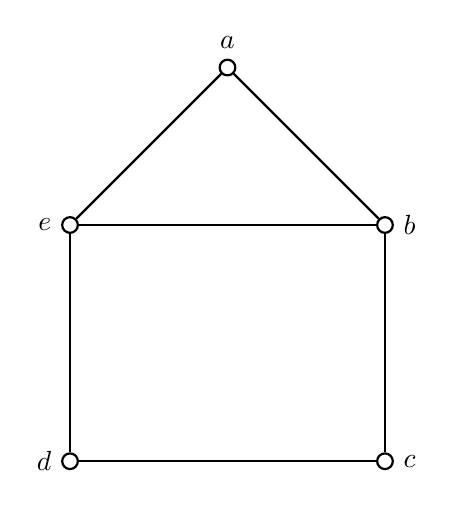
\begin{tikzpicture}
[nodedecorate/.style={shape=circle,inner sep=2pt,draw,thick},%
  linedecorate/.style={-,thick}]
% nodes or vertices
\node (a) at (0,5) [nodedecorate] {};
\node [above] at (a.north) {$a$};
\node (b) at (2,3) [nodedecorate] {};
\node [right] at (b.east) {$b$};
\node (e) at (-2,3) [nodedecorate] {};
\node [left] at (e.west) {$e$};
\node (c) at (2,0) [nodedecorate] {};
\node [right] at (c.east) {$c$};
\node (d) at (-2,0) [nodedecorate] {};
\node [left] at (d.west) {$d$};
% edges or lines
\path
(a) edge[linedecorate] node {} (b)
(b) edge[linedecorate] node {} (c)
(b) edge[linedecorate] node {} (e)
(c) edge[linedecorate] node {} (d)
(d) edge[linedecorate] node {} (e)
(e) edge[linedecorate] node {} (a);
\end{tikzpicture}
\caption{A house graph.}
\label{fig:introduction:house_graph}
\end{figure}

\begin{exercise}
\label{ex:introduction:house_graph}
Consider the graph in Figure~\ref{fig:introduction:house_graph}.
%
\begin{enumerate}
\item List the vertex and edge sets of the graph.

\item For each vertex, list all vertices that are adjacent to it.

\item Which vertex or vertices have the largest number of adjacent
  vertices? Similarly, which vertex or vertices have the smallest
  number of adjacent vertices?

\item If all edges of the graph are removed, is the resulting figure
  still a graph? Why or why not?

\item If all vertices of the graph are removed, is the resulting
  figure still a graph? Why or why not?
\end{enumerate}
\end{exercise}

\begin{proof}[Solution]
(1) Let $G = (V, E)$ denote the graph in
Figure~\ref{fig:introduction:house_graph}. Then the vertex set of $G$
is $V = \{ a, b, c, d, e \}$. The edge set of $G$ is given by
\begin{equation}
\label{eq:introduction:edges_of_house_graph}
E
=
\{ ab, ae, ba, bc, be, cb, cd, dc, de, ed, eb, ea \}.
\end{equation}
We can also use Sage to construct the graph $G$ and list its vertex
and edge sets:
%
\begin{center}
\fontsize{10pt}{10pt}
\selectfont
\tt
\begin{lstlisting}
sage: G = Graph({"a": ["b", "e"], "b": ["a", "c", "e"], "c": ["b", "d"], \
....: "d": ["c", "e"], "e": ["a", "b", "d"]})
sage: G
Graph on 5 vertices
sage: G.vertices()
['a', 'b', 'c', 'd', 'e']
sage: G.edges(labels=False)
[('a', 'b'), ('a', 'e'), ('b', 'e'), ('c', 'b'), ('c', 'd'), ('e', 'd')]
\end{lstlisting}
\end{center}
%
The graph $G$ is undirected, meaning that we do no impose direction on
any edges. Without any direction on the edges, the edge $ab$ is the
same as the edge $ba$. That is why \texttt{G.edges()} returns six
edges instead of the 12 edges listed
in~(\ref{eq:introduction:edges_of_house_graph}).

(2) Let $\text{adj}(v)$ be the set of all vertices that are adjacent
to $v$. Then we have
%
\begin{align*}
\text{adj}(a) &= \{ b, e \} \\
\text{adj}(b) &= \{ a, c, e \} \\
\text{adj}(c) &= \{ b, d \} \\
\text{adj}(d) &= \{ c, e \} \\
\text{adj}(e) &= \{ a, b, d \}
\end{align*}
%
The vertices adjacent to $v$ are also referred to as its
neighbours. We can use the function \texttt{G.neighbors()} to list all
the neighbours of each vertex.
%
\begin{center}
\fontsize{10pt}{10pt}
\selectfont
\tt
\begin{lstlisting}
sage: G.neighbors("a")
['b', 'e']
sage: G.neighbors("b")
['a', 'c', 'e']
sage: G.neighbors("c")
['b', 'd']
sage: G.neighbors("d")
['c', 'e']
sage: G.neighbors("e")
['a', 'b', 'd']
\end{lstlisting}
\end{center}

(3) Taking the cardinalities of the above five sets, we get
$|\text{adj}(a)| = |\text{adj}(c)| = |\text{adj}(d)| = 2$ and
$|\text{adj}(b)| = |\text{adj}(e)| = 3$. Thus $a$, $c$ and $d$ have
the smallest number of adjacent vertices, while $b$ and $e$ have the
largest number of adjacent vertices.

(4) If all the edges in $G$ are removed, the result is still a graph,
although one without any edges. By definition, the edge set of any
graph is a subset of $V \times V$. Removing all edges of $G$ leaves us
with the empty set $\emptyset$, which is a subset of every set.

(5) Say we remove all of the vertices from the graph in
Figure~\ref{fig:introduction:house_graph} and in the process all edges
are removed as well. The result is that both of the vertex and edge
sets are empty. This is a special graph known as an \emph{empty} or
\emph{null} graph.
\end{proof}

\begin{exercise}
Consider the illustration in
Figure~\ref{fig:introduction:self_loop}. Does
Figure~\ref{fig:introduction:self_loop} represent a graph? Why or why not?
\end{exercise}

\begin{proof}[Solution]
If $V = \{ a, b, c \}$ and $E = \{ aa, bc \}$, it is clear that $E
\subseteq V \times V$. Then $(V, E)$ is a graph. The edge $aa$ is
called a \emph{self-loop} of the graph. In general, any edge of the
form $vv$ is a self-loop.
\end{proof}

\begin{figure}[!htbp]
\centering
\begin{tikzpicture}
[nodedecorate/.style={shape=circle,inner sep=2pt,draw,thick},%
  arrowdecorate/.style={-,thick}]
% nodes or vertices
\node (c) at (-2,0) [nodedecorate] {};
\node [left] at (c.west) {$c$};
\node (b) at (2,0) [nodedecorate] {};
\node [right] at (b.east) {$b$};
\node (a) at (0,2) [nodedecorate] {};
\node [above] at (a.north) {$a$};
% edges or lines
\path
(a) edge[arrowdecorate,loop below,min distance=10mm,out=310,in=230] node {} (a)
(b) edge[arrowdecorate] node {} (c);
\end{tikzpicture}
\caption{A figure with a self-loop.}
\label{fig:introduction:self_loop}
\end{figure}

In Figure~\ref{fig:introduction:house_graph}, the edges $ae$ and $ea$
represent one and the same edge. If we do not consider the direction
of the edges in the graph of
Figure~\ref{fig:introduction:house_graph}, then the graph has six
edges. However, if the direction of each edge is taken into account,
then there are 12 edges as listed
in~(\ref{eq:introduction:edges_of_house_graph}). The following
definition captures the situation where the direction of the edges are
taken into account.

\begin{definition}
\textbf{Directed graphs.}
A \emph{directed edge} is an edge such that one vertex incident with it
is designated as the head vertex and the other incident vertex is
designated as the tail vertex. A directed edge is said to be directed
from its tail to its head. A \emph{directed graph} or \emph{digraph} is
a graph such that each of whose edges is directed.
\end{definition}
\index{graphs!directed}
\index{digraph}

It is important to distinguish a graph $G$ as being directed or
undirected. If $G$ is undirected and $uv \in E(G)$, then $uv$ and $vu$
represent the same edge. In case $G$ is a digraph, then $uv$ and $vu$
are different directed edges.

The edges of a digraph can be visually represented as directed arrows,
similarly to the digraph in
Figure~\ref{fig:introduction:directed_triangle_graph}. The graph in
Figure~\ref{fig:introduction:directed_triangle_graph} has the vertex
set $\{ a, b, c \}$ and the edge set $\{ ab, bc, ca \}$. There is an
arrow from vertex $a$ to vertex $b$, hence $ab$ is in the edge
set. However, there is no arrow from $b$ to $a$, so $ba$ is not in the
edge set of the graph in
Figure~\ref{fig:introduction:directed_triangle_graph}.

\begin{figure}[!htbp]
\centering
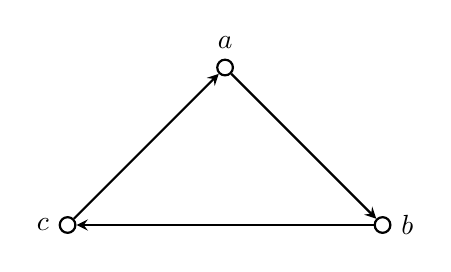
\begin{tikzpicture}
[nodedecorate/.style={shape=circle,inner sep=2pt,draw,thick},%
  arrowdecorate/.style={->,>=stealth,thick}]
% nodes or vertices
\node (c) at (-2,0) [nodedecorate] {};
\node [left] at (c.west) {$c$};
\node (b) at (2,0) [nodedecorate] {};
\node [right] at (b.east) {$b$};
\node (a) at (0,2) [nodedecorate] {};
\node [above] at (a.north) {$a$};
% edges or lines
\path
(a) edge[arrowdecorate] node {} (b)
(b) edge[arrowdecorate] node {} (c)
(c) edge[arrowdecorate] node {} (a);
\end{tikzpicture}
\caption{A triangle as a directed graph.}
\label{fig:introduction:directed_triangle_graph}
\end{figure}

For any vertex $v$ in a graph $G = (V, E)$, the cardinality of
$\text{adj}(v)$ is called the \emph{degree} of $v$ and written as
$\deg(v) = |\text{adj}(v)|$. The degree of $v$ counts the number of
vertices in $G$ that are adjacent to $v$. If $\deg(v) = 0$, we say
that $v$ is an \emph{isolated} vertex. For example, in the graph in
Figure~\ref{fig:introduction:house_graph}, we have $\deg(b) = 3$. For
the graph in Figure~\ref{fig:introduction:directed_triangle_graph}, we
have $\deg(b) = 2$. If $V \neq \emptyset$ and $E = \emptyset$, then
$G$ is a graph consisting entirely of isolated vertices. From
Exercise~\ref{ex:introduction:house_graph} we know that the vertices
$a, c, d$ in Figure~\ref{fig:introduction:house_graph} have the
smallest degree in the graph of that figure, while $b, e$ have the
largest degree. The minimum degree among all vertices in $G$ is
denoted $\delta(G)$, whereas the maximum degree is written as
$\Delta(G)$. Thus, if $G$ denotes the graph in
Figure~\ref{fig:introduction:house_graph} then we have $\delta(G) = 2$
and $\Delta(G) = 3$. In the following Sage session, we construct the
digraph in Figure~\ref{fig:introduction:directed_triangle_graph} and
computes its maximum and minimum number of degrees.
\index{degree of a vertex}

%
\begin{center}
\fontsize{10pt}{10pt}
\selectfont
\tt
\begin{lstlisting}
sage: G = DiGraph({"a": "b", "b": "c", "c": "a"})
sage: G
Digraph on 3 vertices
sage: G.degree("a")
2
sage: G.degree("b")
2
sage: G.degree("c")
2
\end{lstlisting}
\end{center}
%
So for the graph $G$ in
Figure~\ref{fig:introduction:directed_triangle_graph}, we have
$\delta(G) = \Delta(G) = 2$.

The graph $G$ in Figure~\ref{fig:introduction:directed_triangle_graph}
has the special property that its minimum degree is the same as its
maximum degree, i.e. $\delta(G) = \Delta(G)$. Graphs with this
property are referred to as \emph{regular}. An $r$-\emph{regular}
graph is a regular graph each of whose vertices has degree $r$. For
instance, $G$ is a $2$-regular graph. The following result, due to
Euler, counts the total number of degrees in any graph.
\index{graphs!regular}

\begin{theorem}
\label{thm:introduction:degree_sum}
\label{thm:introduction:hand_shaking}
\textbf{Euler.}
If $G = (V, E)$ is a graph, then $\sum_{v \in V} \deg(v) = 2 |E|$.
\end{theorem}
\index{hand-shaking lemma}

This lemma is sometimes called the ``hand-shaking lemma,'' due to its
interpretation as in the following story. Suppose you go into a
room. Suppose there are $n$ people in the room (including yourself)
and some people shake hands with others and some do not. Create the
graph with $n$ vertices, where each vertex is associated with a
different person. Draw an edge between two people if they shook
hands. The degree of a vertex is the number of times that person has
shaken hands (we assume that there are no multiple edges, i.e. that no
two people shake hands twice). The theorem above simply says that the
total number of hand shakes is even. This is ``obvious'' when you look
at it this way since each hand shake is counted twice ($A$ shaking
$B$'s hand is counted, $B$ shaking $A$'s hand, since the sum in the
theorem is over all vertices).

\begin{proof}
Each edge $e = v_1 v_2 \in E$ is incident with two vertices, so $e$ is
counted twice towards the total sum of degrees. The first time, we
count $e$ towards the degree of vertex $v_1$ and the second time we
count $e$ towards the degree of $v_2$.
\end{proof}

As $E \subseteq V \times V$, then $E$ can be the empty set, in which
case the total degree of $G = (V, E)$ is zero. Where $E \neq
\emptyset$, then the total degree of $G$ is greater than zero. By
Theorem~\ref{thm:introduction:degree_sum}, the total degree of $G$ is
non-negative and even. This result is an immediate consequence of
Theorem~\ref{thm:introduction:degree_sum} and is captured in the
following corollary.

\begin{corollary}
\label{cor:introduction:degree_sum_even}
If $G$ is a graph, then its total number of degrees is non-negative
and even.
\end{corollary}

If $G = (V, E)$ is an $r$-regular graph with $n$ vertices and $m$
edges, it is clear by definition of $r$-regular graphs that the total
degree of $G$ is $rn$. By Theorem~\ref{thm:introduction:degree_sum} we
have $2m = rn$ and therefore $m = rn / 2$. This result is captured in
the following corollary.

\begin{corollary}
If $G = (V, E)$ is an $r$-regular graph having $n$ vertices and $m$
edges, then $m = rn / 2$.
\end{corollary}


%%-----------------------------------------------------------------------%%
%%--- Subgraphs and other graph types -----------------------------------%%

\section{Subgraphs and other graph types}


%%-----------------------------------------------------------------------%%

\subsection{Walks, trails, and paths}

If $u$ and $v$ are two vertices in a graph $G$, a $u$-$v$ \emph{walk}
is an alternating sequence of vertices and edges starting with $u$ and
ending at $v$. Consecutive vertices and edges are incident. For the
graph in Figure~\ref{fig:introduction:types_of_walks}, an example of a
walk is an $a$-$e$ walk: $a, b, c, b, e$. In other words, we
start at vertex $a$ and travel to vertex $b$. From $b$, we go to $c$
and then back to $b$ again. Then we end our journey at $e$. Notice
that consecutive vertices in a walk are adjacent to each other. One
can think of vertices as destinations and edges as footpaths, say. We
are allowed to have repeated vertices and edges in a walk. The number
of edges in a walk is called its \emph{length}. For instance, the
walk $a, b, c, b, e$ has length $4$.
\index{walk, in a graph}

\begin{figure}[!htbp]
\centering
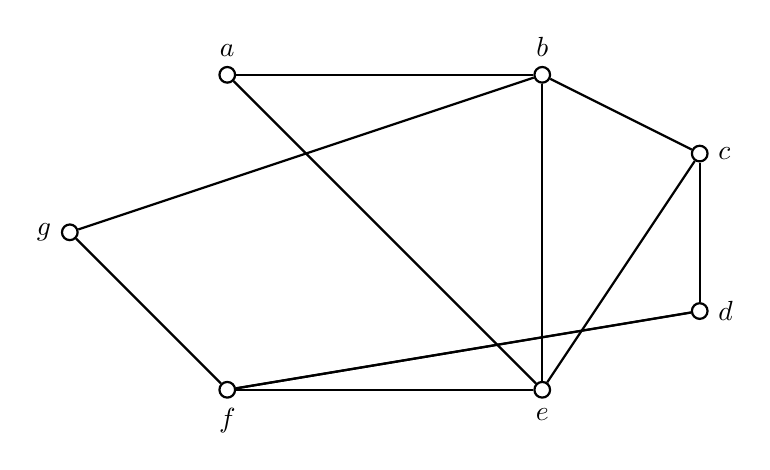
\begin{tikzpicture}
[nodedecorate/.style={shape=circle,inner sep=2pt,draw,thick},%
  linedecorate/.style={-,thick}]
% nodes or vertices
\node (b) at (4,4) [nodedecorate] {};
\node [above] at (b.north) {$b$};
\node (a) at (0,4) [nodedecorate] {};
\node [above] at (a.north) {$a$};
\node (c) at (6,3) [nodedecorate] {};
\node [right] at (c.east) {$c$};
\node (d) at (6,1) [nodedecorate] {};
\node [right] at (d.east) {$d$};
\node (e) at (4,0) [nodedecorate] {};
\node [below] at (e.south) {$e$};
\node (g) at (-2,2) [nodedecorate] {};
\node [left] at (g.west) {$g$};
\node (f) at (0,0) [nodedecorate] {};
\node [below] at (f.south) {$f$};
% edges or lines
\path
(a) edge[linedecorate] node {} (b)
(a) edge[linedecorate] node {} (e)
(b) edge[linedecorate] node {} (c)
(b) edge[linedecorate] node {} (e)
(b) edge[linedecorate] node {} (g)
(c) edge[linedecorate] node {} (d)
(c) edge[linedecorate] node {} (e)
(d) edge[linedecorate] node {} (f)
(d) edge[linedecorate] node {} (f)
(e) edge[linedecorate] node {} (f)
(f) edge[linedecorate] node {} (g);
\end{tikzpicture}
\caption{Walking along a graph.}
\label{fig:introduction:types_of_walks}
\end{figure}

A \emph{trail} is a walk with no repeating edges. For example, the
$a$-$b$ walk $a, b, c, d, f, g, b$ in
Figure~\ref{fig:introduction:types_of_walks} is a trail. It does not
contain any repeated edges, but it contains one repeated vertex,
i.e. $b$. Nothing in the definition of a trail restricts a trail from
having repeated vertices. 
\index{trail}
%\index{circuit}
\index{path}
\index{cycle}

A walk with no repeating vertices is called a \emph{path}. Without any
repeating vertices, a path cannot have repeating edges, hence a path
is also a trail. A path whose start and end vertices are the same is
called a \emph{cycle}. For example, the walk $a, b, c, e, a$
in Figure~\ref{fig:introduction:types_of_walks} is a path and a cycle.
A walk which has no repeated edges and 
the start and end vertices are the same, but otherwise has no 
repeated vertices, is 
%a \emph{circuit}, otherwise known as 
a \emph{closed path} (with apologies for
slightly abusing terminology)\footnote{A closed path in a graph is
 sometimes also called a circuit. Since that terminology 
unfortunately conflicts with the closely related notion of a circuit
of a matroid, we do not use it here.}. Thus the walk $a, b, e, a$ 
in Figure~\ref{fig:introduction:types_of_walks} is a
closed path. It is easy to see that if you remove any edge
from a cycle then the resulting walk contains no closed paths.

\begin{exercise}
Consider the graph in Figure~\ref{fig:introduction:types_of_walks}.
%
\begin{enumerate}
\item Find two distinct walks that are not trails and determine their
  lengths.

\item Find two distinct trails that are not paths and determine their
  lengths.

\item Find two distinct paths and determine their lengths.

\item Find a closed path that is not a cycle.

\item
Find a closed path $C$ which has an edge $e$ such that
$C-e$ contains a cycle.
\end{enumerate}
\end{exercise}

\begin{proof}[Solution]
(1) Here are two distinct walks that are not trails:
$w_1: g, b, e, a, b, e$ and $w_2: f, d, c, e, f, d$. The length of
walk $w_1$ is 5 and the length of walk $w_2$ is also 5.

(2) Here are two distinct trails that are not paths:
$t_1: a, b, c, d, f$ and $t_2: b, e, f, d, c$. The length of trail
$t_1$ is 4 and the length of trail $t_2$ is also 4.

(3) Here are two distinct paths: $p_1: a, b, c, d, f, e$ and
$p_2: g, b, a, e, f, d$. The length of path $p_1$ is 5 and the length
of path $p_2$ is also 5.

(4) Here is a closed path that is not a cycle: $d, c, e, b, a, e, f, d$.
\end{proof}

A graph is said to be \emph{connected} if for every pair of distinct
vertices $u, v$ there is a $u$-$v$ path joining them. A graph that is
not connected is referred to as \emph{disconnected}. The empty graph
is disconnected and so is any non-empty graph with an isolated
vertex. However, the graph in
Figure~\ref{fig:introduction:directed_triangle_graph} is
connected. A \emph{geodesic path} or \emph{shortest path} between two
distinct vertices $u,v$ of a graph is a $u$-$v$ path of minimum
length. A non-empty graph may have several shortest paths between some
distinct pair of vertices. For the graph in
Figure~\ref{fig:introduction:types_of_walks}, both $a,b,c$ and $a,e,c$
are geodesic paths between $a$ and $c$.
\index{path!geodesic}
\index{graph!connected}

\begin{exercise}
Determine whether or not the graph in
Figure~\ref{fig:introduction:types_of_walks} is connected. Find a
shortest path from $g$ to $d$.
\end{exercise}

\begin{proof}[Solution]
In the following Sage session, we first construct the graph in
Figure~\ref{fig:introduction:types_of_walks} and use the method
\verb!is_connected()! to determine whether or not the graph is
connected. Finally, we use the method \verb!shortest_path()! to find
a geodesic path between $g$ and $d$.
%
\begin{center}
\fontsize{10pt}{10pt}
\selectfont
\tt
\begin{lstlisting}
sage: g = Graph({"a": ["b", "e"], "b": ["a", "g", "e", "c"], \
....: "c": ["b", "e", "d"], "d": ["c", "f"], "e": ["f", "a", "b", "c"], \
....: "f": ["g", "d", "e"], "g": ["b", "f"]})
sage: g.is_connected()
True
sage: g.shortest_path("g", "d")
['g', 'f', 'd']
\end{lstlisting}
\end{center}
%
This shows that $g, f, d$ is a shortest path from $g$ to $d$. In fact,
any other $g$-$d$ path has length greater than $2$, so we can say that
$g, f, d$ is the shortest path between $g$ and $d$.
\end{proof}

We will explain Dijkstra's algorithm in
Chapter~\ref{chap:graph_algorithms}, which gives one of the best
algorithms for finding shortest paths between two vertices in a
connected graph. What is very remarkable is that, at the present state
of knowledge, finding the shortest path from a vertex $v$ to a
\emph{particular} (but arbitrarily given) vertex $w$ appears to be as
hard as finding the shortest path from a vertex $v$ to \emph{all}
other vertices in the graph!


%%-----------------------------------------------------------------------%%

\subsection{Subgraphs, complete and bipartite graphs}

\begin{definition}
Let $G$ be a graph with vertex set $V(G)$ and edge set
$E(G)$. Consider a graph $H$ such that $V(H) \subseteq V(G)$ and $E(H)
\subseteq E(G)$. Furthermore, if $uv \in E(H)$ then $u,v \in
V(H)$. Then $H$ is called a \emph{subgraph} of $G$ and $G$ is referred
to as a \emph{supergraph} of $H$.
\end{definition}
\index{subgraph}
\index{supergraph}

Starting from $G$, one can obtain its subgraph $H$ by deleting edges
and/or vertices from $G$. Note that when a vertex $v$ is removed from
$G$, then all edges incident with $v$ are also removed. If $V(H) =
V(G)$, then $H$ is called a \emph{spanning} subgraph of $G$. In
Figure~\ref{fig:introduction:star_subgraph}, let $G$ be the left-hand
side graph and let $H$ be the right-hand side graph. Then it is clear
that $H$ is a spanning subgraph of $G$. To obtain a spanning subgraph
from a given graph, we delete edges from the given graph.
\index{spanning subgraph}

\begin{figure}[!htbp]
\centering
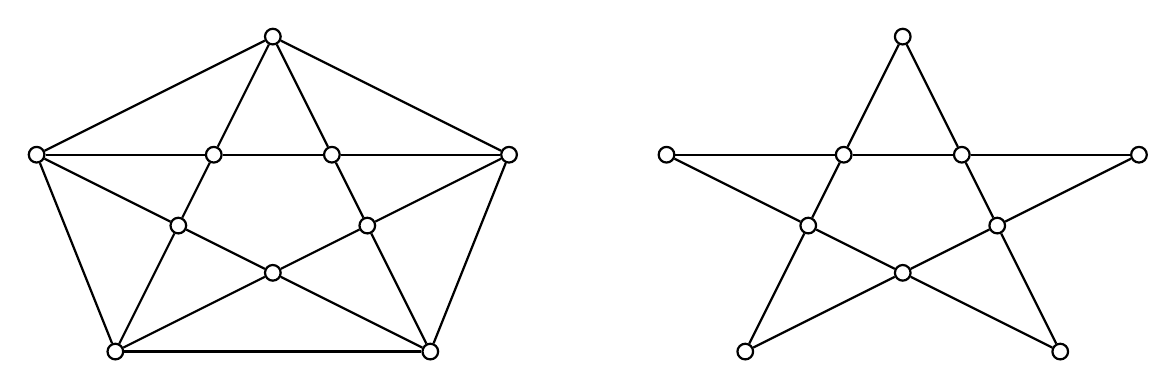
\begin{tikzpicture}
[nodedecorate/.style={shape=circle,inner sep=2pt,draw,thick},%
  linedecorate/.style={-,thick}]
%%% pentagon with star and inner pentagon
% nodes or vertices
\node (a) at (-2,0) [nodedecorate] {};
\node (b) at (2,0) [nodedecorate] {};
\node (c) at (-3,2.5) [nodedecorate] {};
\node (d) at (3,2.5) [nodedecorate] {};
\node (e) at (0,4) [nodedecorate] {};
\node (f) at (-0.75,2.5) [nodedecorate] {};
\node (g) at (-1.2,1.6) [nodedecorate] {};
\node (h) at (0,1) [nodedecorate] {};
\node (i) at (1.2,1.6) [nodedecorate] {};
\node (j) at (0.75,2.5) [nodedecorate] {};
% edges or lines
\path
(a) edge[linedecorate] node {} (b)
(a) edge[linedecorate] node {} (c)
(a) edge[linedecorate] node {} (g)
(a) edge[linedecorate] node {} (h)
(b) edge[linedecorate] node {} (d)
(b) edge[linedecorate] node {} (h)
(b) edge[linedecorate] node {} (i)
(c) edge[linedecorate] node {} (e)
(c) edge[linedecorate] node {} (f)
(c) edge[linedecorate] node {} (g)
(d) edge[linedecorate] node {} (e)
(d) edge[linedecorate] node {} (i)
(d) edge[linedecorate] node {} (j)
(e) edge[linedecorate] node {} (f)
(e) edge[linedecorate] node {} (j)
(f) edge[linedecorate] node {} (g)
(f) edge[linedecorate] node {} (j)
(g) edge[linedecorate] node {} (h)
(h) edge[linedecorate] node {} (i)
(i) edge[linedecorate] node {} (j);
%
%%% star and inner pentagon
% nodes or vertices
\node (a2) at (6,0) [nodedecorate] {};
\node (b2) at (10,0) [nodedecorate] {};
\node (c2) at (5,2.5) [nodedecorate] {};
\node (d2) at (11,2.5) [nodedecorate] {};
\node (e2) at (8,4) [nodedecorate] {};
\node (f2) at (7.25,2.5) [nodedecorate] {};
\node (g2) at (6.8,1.6) [nodedecorate] {};
\node (h2) at (8,1) [nodedecorate] {};
\node (i2) at (9.2,1.6) [nodedecorate] {};
\node (j2) at (8.75,2.5) [nodedecorate] {};
% edges or lines
\path
(a2) edge[linedecorate] node {} (g2)
(a2) edge[linedecorate] node {} (h2)
(b2) edge[linedecorate] node {} (h2)
(b2) edge[linedecorate] node {} (i2)
(c2) edge[linedecorate] node {} (f2)
(c2) edge[linedecorate] node {} (g2)
(d2) edge[linedecorate] node {} (i2)
(d2) edge[linedecorate] node {} (j2)
(e2) edge[linedecorate] node {} (f2)
(e2) edge[linedecorate] node {} (j2)
(f2) edge[linedecorate] node {} (g2)
(f2) edge[linedecorate] node {} (j2)
(g2) edge[linedecorate] node {} (h2)
(h2) edge[linedecorate] node {} (i2)
(i2) edge[linedecorate] node {} (j2);
\end{tikzpicture}
\caption{A graph and one of its subgraphs.}
\label{fig:introduction:star_subgraph}
\end{figure}

\index{graph!complete}
We now consider several standard classes of graphs. The \emph{complete}
graph $K_n$ on $n$ vertices is a graph such that any two distinct
vertices are adjacent. As $|V(K_n)| = n$, then $|E(K_n)|$ is
equivalent to the total number of 2-combinations from a set of $n$
objects:
\[
|E(K_n)|
=
\binom{n}{2}
=
\frac{n(n-1)}{2}
\]
Thus for any graph $G$ with $n$ vertices, its total number of edges
$|E(G)|$ is bounded above by
\[
|E(G)|
\leq
\frac{n(n - 1)}{2}
\]
Figure~\ref{fig:introduction:five_complete_graphs} shows complete
graphs each of whose total number of vertices is bounded by
$1 \leq n \leq 5$. The complete graph $K_1$ has one vertex with
no edges. It is also called the \emph{trivial} graph.
\index{graph!trivial}

\begin{figure}[!htbp]
\centering
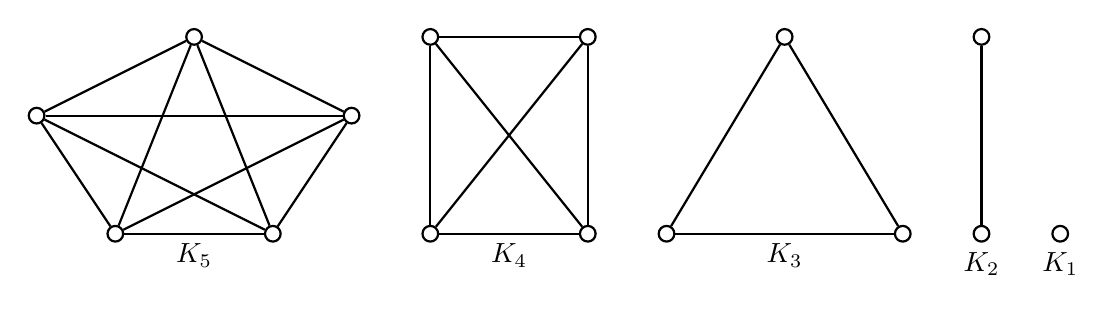
\begin{tikzpicture}
[nodedecorate/.style={shape=circle,inner sep=2pt,draw,thick},%
  linedecorate/.style={-,thick}]
%%% complete graph K_5
% nodes or vertices
\node (a) at (-1,0) [nodedecorate] {};
\node (b) at (1,0) [nodedecorate] {};
\node (c) at (-2,1.5) [nodedecorate] {};
\node (d) at (2,1.5) [nodedecorate] {};
\node (e) at (0,2.5) [nodedecorate] {};
% edges or lines
\path
(a) edge[linedecorate] node[below] {$K_5$} (b)
(a) edge[linedecorate] node {} (c)
(a) edge[linedecorate] node {} (d)
(a) edge[linedecorate] node {} (e)
(b) edge[linedecorate] node {} (c)
(b) edge[linedecorate] node {} (d)
(b) edge[linedecorate] node {} (e)
(c) edge[linedecorate] node {} (d)
(c) edge[linedecorate] node {} (e)
(d) edge[linedecorate] node {} (e);
%
%%% complete graph K_4
% nodes or vertices
\node (a) at (3,0) [nodedecorate] {};
\node (b) at (5,0) [nodedecorate] {};
\node (c) at (3,2.5) [nodedecorate] {};
\node (d) at (5,2.5) [nodedecorate] {};
% edges or lines
\path
(a) edge[linedecorate] node[below] {$K_4$} (b)
(a) edge[linedecorate] node {} (c)
(a) edge[linedecorate] node {} (d)
(b) edge[linedecorate] node {} (c)
(b) edge[linedecorate] node {} (d)
(c) edge[linedecorate] node {} (d);
%
%%% complete graph K_3
% nodes or vertices
\node (a) at (6,0) [nodedecorate] {};
\node (b) at (9,0) [nodedecorate] {};
\node (c) at (7.5,2.5) [nodedecorate] {};
% edges or lines
\path
(a) edge[linedecorate] node[below] {$K_3$} (b)
(a) edge[linedecorate] node {} (c)
(b) edge[linedecorate] node {} (c);
%
%%% complete graph K_2
% nodes or vertices
\node (a) at (10,0) [nodedecorate] {};
\node [below] at (a.south) {$K_2$};
\node (b) at (10,2.5) [nodedecorate] {};
% edges or lines
\path
(a) edge[linedecorate] node {} (b);
%
%%% complete graph K_1
% nodes or vertices
\node (a) at (11,0) [nodedecorate] {};
\node [below] at (a.south) {$K_1$};
\end{tikzpicture}
\caption{Complete graphs $K_n$ for $1 \leq n \leq 5$.}
\label{fig:introduction:five_complete_graphs}
\end{figure}

\index{graph!cycle}
The \emph{cycle} graph on $n \geq 3$ vertices, denoted $C_n$, is the
connected $2$-regular graph on $n$ vertices. Each vertex in $C_n$ has
degree exactly $2$ and $C_n$ is
connected. Figure~\ref{fig:introduction:four_cycle_graphs} shows
cycles graphs $C_n$ where $3 \leq n \leq 6$. The \emph{path} on
$n \geq 1$ vertices is denoted $P_n$. For $n = 1, 2$ we have
$P_1 = K_1$ and $P_2 = K_2$. Where $n \geq 3$, then $P_n$ is a
spanning subgraph of $C_n$ obtained by deleting one edge.

\begin{figure}[!htbp]
\centering
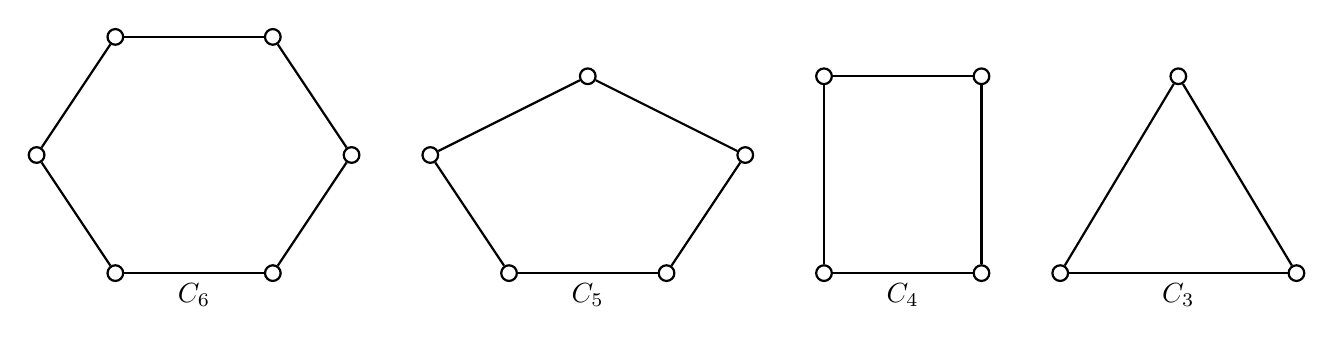
\begin{tikzpicture}
[nodedecorate/.style={shape=circle,inner sep=2pt,draw,thick},%
  linedecorate/.style={-,thick}]
%%% cycle graph C_6
% nodes or vertices
\node (a) at (-6,0) [nodedecorate] {};
\node (b) at (-4,0) [nodedecorate] {};
\node (c) at (-7,1.5) [nodedecorate] {};
\node (d) at (-3,1.5) [nodedecorate] {};
\node (e) at (-6,3) [nodedecorate] {};
\node (f) at (-4,3) [nodedecorate] {};
% edges or lines
\path
(a) edge[linedecorate] node[below] {$C_6$} (b)
(a) edge[linedecorate] node {} (c)
(b) edge[linedecorate] node {} (d)
(c) edge[linedecorate] node {} (e)
(d) edge[linedecorate] node {} (f)
(e) edge[linedecorate] node {} (f);
%
%%% cycle graph C_5
% nodes or vertices
\node (a) at (-1,0) [nodedecorate] {};
\node (b) at (1,0) [nodedecorate] {};
\node (c) at (-2,1.5) [nodedecorate] {};
\node (d) at (2,1.5) [nodedecorate] {};
\node (e) at (0,2.5) [nodedecorate] {};
% edges or lines
\path
(a) edge[linedecorate] node[below] {$C_5$} (b)
(a) edge[linedecorate] node {} (c)
(b) edge[linedecorate] node {} (d)
(c) edge[linedecorate] node {} (e)
(d) edge[linedecorate] node {} (e);
%
%%% cycle graph C_4
% nodes or vertices
\node (a) at (3,0) [nodedecorate] {};
\node (b) at (5,0) [nodedecorate] {};
\node (c) at (3,2.5) [nodedecorate] {};
\node (d) at (5,2.5) [nodedecorate] {};
% edges or lines
\path
(a) edge[linedecorate] node[below] {$C_4$} (b)
(a) edge[linedecorate] node {} (c)
(b) edge[linedecorate] node {} (d)
(c) edge[linedecorate] node {} (d);
%
%%% cycle graph C_3
% nodes or vertices
\node (a) at (6,0) [nodedecorate] {};
\node (b) at (9,0) [nodedecorate] {};
\node (c) at (7.5,2.5) [nodedecorate] {};
% edges or lines
\path
(a) edge[linedecorate] node[below] {$C_3$} (b)
(a) edge[linedecorate] node {} (c)
(b) edge[linedecorate] node {} (c);
\end{tikzpicture}
\caption{Cycle graphs $C_n$ for $3 \leq n \leq 6$.}
\label{fig:introduction:four_cycle_graphs}
\end{figure}

A \emph{bipartite} graph $G$ is a graph with at least two
vertices such that $V(G)$ can be split into two disjoint subsets $V_1$
and $V_2$, both non-empty. Every edge $uv \in E(G)$ is such that
$u \in V_1$ and $v \in V_2$, or $v \in V_1$ and $u \in V_2$. The
\emph{complete bipartite} graph $K_{m,n}$ is the bipartite graph whose
vertex set is partitioned into two non-empty disjoint sets $V_1$ and
$V_2$ with $|V_1| = m$ and $|V_2| = n$. Any vertex in $V_1$ is
adjacent to each vertex in $V_2$, and any two distinct vertices in
$V_i$ are not adjacent to each other. If $m = n$, then $K_{n,n}$ is
$n$-regular. Where $m = 1$ then $K_{1,n}$ is called the \emph{star}
graph. Figure~\ref{fig:introduction:bipartite_complete_bipartite_graphs}
shows a bipartite graph together with the complete bipartite graphs
$K_{4,3}$ and $K_{3,3}$, and the star graph $K_{1,4}$.

\begin{figure}[!htbp]
\centering
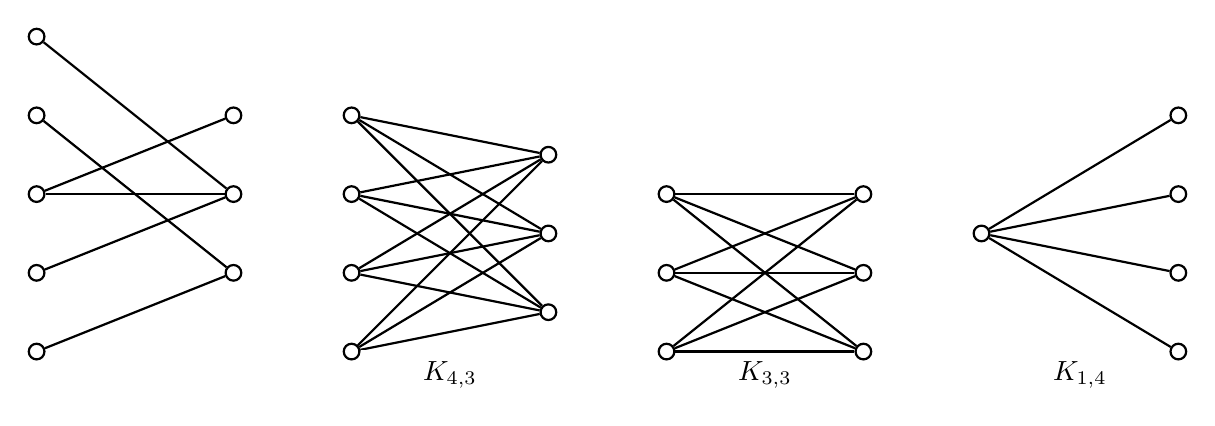
\begin{tikzpicture}
[nodedecorate/.style={shape=circle,inner sep=2pt,draw,thick},%
  linedecorate/.style={-,thick}]
%%% bipartite graph
% nodes or vertices
\node (a) at (0,0) [nodedecorate] {};
\node (b) at (0,1) [nodedecorate] {};
\node (c) at (0,2) [nodedecorate] {};
\node (d) at (0,3) [nodedecorate] {};
\node (e) at (0,4) [nodedecorate] {};
\node (f) at (2.5,3) [nodedecorate] {};
\node (g) at (2.5,2) [nodedecorate] {};
\node (h) at (2.5,1) [nodedecorate] {};
% edges or lines
\path
(a) edge[linedecorate] node {} (h)
(b) edge[linedecorate] node {} (g)
(c) edge[linedecorate] node {} (g)
(c) edge[linedecorate] node {} (f)
(d) edge[linedecorate] node {} (h)
(e) edge[linedecorate] node {} (g);
%
%%% complete bipartite graph K_{4,3}
% nodes or vertices
\node (a) at (4,0) [nodedecorate] {};
\node (b) at (4,1) [nodedecorate] {};
\node (c) at (4,2) [nodedecorate] {};
\node (d) at (4,3) [nodedecorate] {};
\node (e) at (6.5,2.5) [nodedecorate] {};
\node (f) at (6.5,1.5) [nodedecorate] {};
\node (g) at (6.5,0.5) [nodedecorate] {};
\node (h) at (6.5,0) [nodedecorate,color=white] {};
% edges or lines
\path
(a) edge[linedecorate] node {} (e)
(a) edge[linedecorate] node {} (f)
(a) edge[linedecorate] node {} (g)
(a) edge[linedecorate,color=white] node[below,color=black] {$K_{4,3}$} (h)
(b) edge[linedecorate] node {} (e)
(b) edge[linedecorate] node {} (f)
(b) edge[linedecorate] node {} (g)
(c) edge[linedecorate] node {} (e)
(c) edge[linedecorate] node {} (f)
(c) edge[linedecorate] node {} (g)
(d) edge[linedecorate] node {} (e)
(d) edge[linedecorate] node {} (f)
(d) edge[linedecorate] node {} (g);
%
%%% complete bipartite graph K_{3,3}
% nodes or vertices
\node (a) at (8,0) [nodedecorate] {};
\node (b) at (8,1) [nodedecorate] {};
\node (c) at (8,2) [nodedecorate] {};
\node (d) at (10.5,2) [nodedecorate] {};
\node (e) at (10.5,1) [nodedecorate] {};
\node (f) at (10.5,0) [nodedecorate] {};
% edges or lines
\path
(a) edge[linedecorate] node {} (d)
(a) edge[linedecorate] node {} (e)
(a) edge[linedecorate] node[below] {$K_{3,3}$} (f)
(b) edge[linedecorate] node {} (d)
(b) edge[linedecorate] node {} (e)
(b) edge[linedecorate] node {} (f)
(c) edge[linedecorate] node {} (d)
(c) edge[linedecorate] node {} (e)
(c) edge[linedecorate] node {} (f);
%
%%% star graph K_{1,4}
% nodes or vertices
\node (a) at (12,1.5) [nodedecorate] {};
\node (b) at (14.5,3) [nodedecorate] {};
\node (c) at (14.5,2) [nodedecorate] {};
\node (d) at (14.5,1) [nodedecorate] {};
\node (e) at (14.5,0) [nodedecorate] {};
\node (f) at (12,0) [nodedecorate,color=white] {};
% edges or lines
\path
(a) edge[linedecorate] node {} (b)
(a) edge[linedecorate] node {} (c)
(a) edge[linedecorate] node {} (d)
(a) edge[linedecorate] node {} (e)
(f) edge[linedecorate,color=white] node[below,color=black] {$K_{1,4}$} (e);
\end{tikzpicture}
\caption{Bipartite, complete bipartite and star graphs.}
\label{fig:introduction:bipartite_complete_bipartite_graphs}
\end{figure}

As an example of $K_{3,3}$, suppose that there are $3$ boys and $3$
girls dancing in a room. The boys and girls naturally partition the
set of all people in the room. Construct a graph having $6$ vertices,
each vertex corresponding to a person in the room, and draw an edge
form one vertex to another if the two people dance together. If each
girl dances three times, once with with each of the three boys, then
the resulting graph is $K_{3,3}$.

%%--- Representing graphs as matrices -----------------------------------%%

\section{Representing graphs as matrices}

Representing a graph as a matrix is very inefficient in some cases
and not so in other cases. For example, if you walk into a large room
full of people and you consider the ``hand-shaking graph'' that we
discussed in connection with
Theorem~\ref{thm:introduction:hand_shaking}. If not many people shake
hands in the room, then it is a waste of time to have to record all
the hand-shakes and also all the ``non-hand-shakes.'' This is
basically what the adjacency matrix does. In this kind of ``sparse
graph'' situation, it would
be much easier to simply record the hand-shakes as a Python dictionary.

If $G$ is an undirected graph with vertices $V=\{v_1,\dots, v_n\}$
and edges $E$ then the 
{\it adjacency matrix} of $G$ is the $n\times n$ matrix $A=(a_{ij})$ 
defined by

\[
a_{ij}=
\left\{
\begin{array}{ll}
1, & {\rm if}\ (v_i,v_j)\in E,\\
0, &{\rm otherwise}.
\end{array}
\right.
\]
If $G$ is an undirected graph then $A$ 
is a symmetric matrix.

If $G$ is a directed graph with vertices $V=\{v_1,\dots, v_n\}$
and edges $E$ then the $(0,-1,1)$-{\it adjacency matrix} 
of $G$ is the $n\times n$ matrix $A=(a_{ij})$ 
defined by
\index{adjacency matrix} 

\[
a_{ij}=
\left\{
\begin{array}{rl}
1, & {\rm if}\ (v_i,v_j)\in E,\\
-1, & {\rm if}\ (v_j,v_i)\in E,\\
0, &{\rm otherwise}.
\end{array}
\right.
\]

%\begin{itemize}
%\item what's a matrix?
%
%\item adjacency matrices for digraphs
%
%\item adjacency matrices for undirected graphs
%\end{itemize}

%\begin{example}
For example, Sage allows you to easily compute an adjacency matrix.

%
\begin{center}
\fontsize{10pt}{10pt}
\selectfont
\tt
\begin{lstlisting}
sage: C6 = Graph({1: [2, 4], 2: [1, 3], 3: [2, 6], 4: [1, 5], \
....: 5: [4, 6], 6: [3, 5]})
sage: G1 = Graph({"a": ["b", "c"], "b": ["a", "d"], "c": ["a", "e"], \
....: "d": ["b", "f"], "e": ["c", "f"], "f": ["d", "e"]})
sage: G1.adjacency_matrix()
[0 1 0 1 0 0]
[1 0 1 0 0 0]
[0 1 0 0 0 1]
[1 0 0 0 1 0]
[0 0 0 1 0 1]
[0 0 1 0 1 0]
sage: G2.adjacency_matrix()
[0 1 1 0 0 0]
[1 0 0 1 0 0]
[1 0 0 0 1 0]
[0 1 0 0 0 1]
[0 0 1 0 0 1]
[0 0 0 1 1 0]
sage: G1.adjacency_matrix()^2
[2 0 1 0 1 0]
[0 2 0 1 0 1]
[1 0 2 0 1 0]
[0 1 0 2 0 1]
[1 0 1 0 2 0]
[0 1 0 1 0 2]
\end{lstlisting}
\end{center}
%
%\end{example}


\begin{theorem}
Let $G$ be a graph of order $n$ and $\mathbf{A}$ the adjacency matrix
of $G$. For each positive integer $k$, the $i$-$j$ entry of
$\mathbf{A}^k$ counts the number of $v_i$-$v_j$ walks of length $k$.
\end{theorem}

There is an analog of the adjacency matrix for edges.
If $G$ is an undirected graph with edges $E=\{e_1,\dots, e_m\}$
and vertices $V=\{v_1,\dots,v_m\}$ then the 
{\it incidence matrix} of $G$ is the $n\times m$ matrix $B=(b_{ij})$ 
defined by

\[
b_{ij}=
\left\{
\begin{array}{ll}
1, & {\rm if}\ v_i\ {\rm incident\ to}\ e_j,\\
0, &{\rm otherwise}.
\end{array}
\right.
\]
If $G$ is a directed graph with edges $E=\{e_1,\dots, e_m\}$
and vertices $V=\{v_1,\dots,v_m\}$ then the 
{\it incidence matrix} of $G$ is the $n\times m$ matrix $B=(b_{ij})$ 
defined by
\index{incidence matrix}

\[
b_{ij}=
\left\{
\begin{array}{rl}
-1, & {\rm if}\ v_i\ {\rm incident\ to}\ e_j,\ e_j \ {\rm leaves}\
v_i\\
1, & {\rm if}\ v_i\ {\rm incident\ to}\ e_j,\ e_j \ {\rm enters}\ v_i\\
0, &{\rm otherwise}.
\end{array}
\right.
\]

Sage allows you to compute the incidence matrix of a 
graph.

%\begin{example}
%
\begin{center}
\fontsize{9pt}{9pt}
\selectfont
\tt
\begin{lstlisting}
sage: G = Graph({1: [2, 4], 2: [1, 3], 3: [2, 6], 4: [1, 5], 5: [4, 6], 6: [3, 5]})
sage: G.incidence_matrix()
[-1 -1  0  0  0  0]
[ 0  1 -1  0  0  0]
[ 0  0  1 -1  0  0]
[ 1  0  0  0 -1  0]
[ 0  0  0  0  1 -1]
[ 0  0  0  1  0  1]
\end{lstlisting}
\end{center}
%
%\end{example}


%%-----------------------------------------------------------------------%%
%%--- Isomorphic graphs -------------------------------------------------%%

\section{Isomorphic graphs}

Determining whether or not two graphs are, in some sense, the ``same''
is a hard but important problem.

\begin{definition}
\textbf{Isomorphic graphs.}
Two graphs $G$ and $H$ are \emph{isomorphic} if there is a bijection
$f: V(G) \longrightarrow V(H)$ such that whenever $uv \in E(G)$ then
$f(u) f(v) \in E(H)$. The function $f$ is an \emph{isomorphism}
between $G$ and $H$. Otherwise, $G$ and $H$ are non-isomorphic. If
$G$ and $H$ are isomorphic, we write $G \cong H$.
\end{definition}
\index{graphs!isomorphic}

A graph $G$ is isomorphic to a graph $H$ if these two graphs can be
labelled in such a way that if $u$ and $v$ are adjacent in $G$, then
their counterparts in $V(H)$ are also adjacent in $H$. To determine
whether or not two graphs are isomorphic is to determine if they are
structurally equivalent. Graphs $G$ and $H$ may be drawn differently
so that they seem different. However, if $G \cong H$ then the
isomorphism $f: V(G) \longrightarrow V(H)$ shows that both of these
graphs are fundamentally the same. In particular, the order and size
of $G$ are equal to those of $H$, the isomorphism $f$ preserves
adjacencies, and $\deg(v) = \deg(f(v))$ for all $v \in G$. Since $f$
preserves adjacencies, then adjacencies along a given geodesic path
are preserved as well. That is, if $v_1, v_2, v_3, \dots, v_k$ is a
shortest path between $v_1, v_k \in V(G)$, then
$f(v_1), f(v_2), f(v_3), \dots, f(v_k)$ is a geodesic path between
$f(v_1), f(v_k) \in V(H)$.

%% Hopefully later we can discuss ``canonical labeling''
%% and how that gives rise to isomorphism/automorphism
%% testing methods???

\begin{figure}[!htbp]
\centering
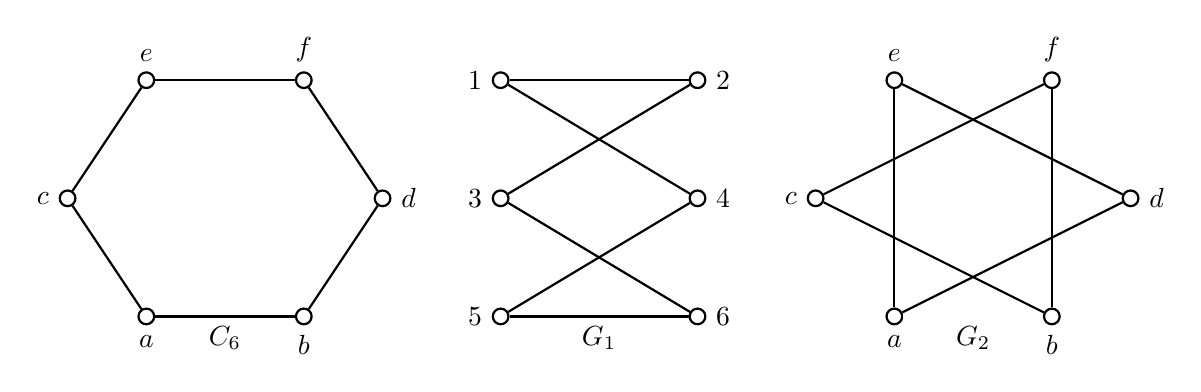
\begin{tikzpicture}
[nodedecorate/.style={shape=circle,inner sep=2pt,draw,thick},%
  linedecorate/.style={-,thick}]
%%% cycle graph C_6
% nodes or vertices
\node (a) at (0,0) [nodedecorate] {};
\node [below] at (a.south) {$a$};
\node (b) at (2,0) [nodedecorate] {};
\node [below] at (b.south) {$b$};
\node (c) at (-1,1.5) [nodedecorate] {};
\node [left] at (c.west) {$c$};
\node (d) at (3,1.5) [nodedecorate] {};
\node [right] at (d.east) {$d$};
\node (e) at (0,3) [nodedecorate] {};
\node [above] at (e.north) {$e$};
\node (f) at (2,3) [nodedecorate] {};
\node [above] at (f.north) {$f$};
% edges or lines
\path
(a) edge[linedecorate] node[below] {$C_6$} (b)
(a) edge[linedecorate] node {} (c)
(b) edge[linedecorate] node {} (d)
(c) edge[linedecorate] node {} (e)
(d) edge[linedecorate] node {} (f)
(e) edge[linedecorate] node {} (f);
%
%%% graph G_1 that is isomorphic to C_6
% nodes or vertices
\node (1) at (4.5,3) [nodedecorate] {};
\node [left] at (1.west) {$1$};
\node (2) at (7,3) [nodedecorate] {};
\node [right] at (2.east) {$2$};
\node (3) at (4.5,1.5) [nodedecorate] {};
\node [left] at (3.west) {$3$};
\node (4) at (7,1.5) [nodedecorate] {};
\node [right] at (4.east) {$4$};
\node (5) at (4.5,0) [nodedecorate] {};
\node [left] at (5.west) {$5$};
\node (6) at (7,0) [nodedecorate] {};
\node [right] at (6.east) {$6$};
% edges or lines
\path
(1) edge[linedecorate] node {} (2)
(1) edge[linedecorate] node {} (4)
(3) edge[linedecorate] node {} (2)
(3) edge[linedecorate] node {} (6)
(5) edge[linedecorate] node {} (4)
(5) edge[linedecorate] node[below] {$G_1$} (6);
%
%%% graph G_2 that is non-isomorphic to C_6
% nodes or vertices
\node (a) at (9.5,0) [nodedecorate] {};
\node [below] at (a.south) {$a$};
\node (b) at (11.5,0) [nodedecorate] {};
\node [below] at (b.south) {$b$};
\node (c) at (8.5,1.5) [nodedecorate] {};
\node [left] at (c.west) {$c$};
\node (d) at (12.5,1.5) [nodedecorate] {};
\node [right] at (d.east) {$d$};
\node (e) at (9.5,3) [nodedecorate] {};
\node [above] at (e.north) {$e$};
\node (f) at (11.5,3) [nodedecorate] {};
\node [above] at (f.north) {$f$};
% edges or lines
\path
(a) edge[linedecorate] node {} (d)
(a) edge[linedecorate] node {} (e)
(b) edge[linedecorate] node {} (c)
(b) edge[linedecorate] node {} (f)
(c) edge[linedecorate] node {} (f)
(d) edge[linedecorate] node {} (e)
(a) edge[linedecorate,color=white] node[below,color=black] {$G_2$} (b);
\end{tikzpicture}
\caption{Isomorphic and non-isomorphic graphs.}
\label{fig:introduction:isomorphic_graphs}
\end{figure}

\begin{exercise}
Consider the graphs in
Figure~\ref{fig:introduction:isomorphic_graphs}. Which pair of graphs
are isomorphic, and which two graphs are non-isomorphic?
\end{exercise}

\begin{proof}[Solution]
If \verb!G! is a Sage graph, one can use the method
\verb!G.is_isomorphic()! to determine whether or not the graph
\verb!G! is isomorphic to another graph. The following Sage session
illustrates how to use \verb!G.is_isomorphic()!.
%
\begin{center}
\fontsize{10pt}{10pt}
\selectfont
\tt
\begin{lstlisting}
sage: C6 = Graph({"a": ["b", "c"], "b": ["a", "d"], "c": ["a", "e"], \
....: "d": ["b", "f"], "e": ["c", "f"], "f": ["d", "e"]})
sage: G1 = Graph({1: [2, 4], 2: [1, 3], 3: [2, 6], 4: [1, 5], \
....: 5: [4, 6], 6: [3, 5]})
sage: G2 = Graph({"a": ["d", "e"], "b": ["c", "f"], "c": ["b", "f"], \
....: "d": ["a", "e"], "e": ["a", "d"], "f": ["b", "c"]})
sage: C6.is_isomorphic(G1)
True
sage: C6.is_isomorphic(G2)
False
sage: G1.is_isomorphic(G2)
False
\end{lstlisting}
\end{center}
%
Thus, for the graphs $C_6$, $G_1$ and $G_2$ in
Figure~\ref{fig:introduction:isomorphic_graphs}, $C_6$ and $G_1$ are
isomorphic, but $G_1$ and $G_2$ are not isomorphic.
\end{proof}



\subsection{Adjacency matrices}

Two $n\times n$ matrices $A_1$ and $A_2$ are {\it permutation
equivalent} if there is a permutation matrix $P$ such
that $A_1=PA_2P^{-1}$. In other words, $A_1$ is the same as $A_2$
after a suitable reordering of the rows and a corresponding 
reordiering of the columns.
\index{permutation equivalent}
This notion of permutation equivalence is an equivalence relation.

To show two undirected graphs are isomorphic depends on the following result.

\begin{theorem}
Consider two directed or undirected graphs $G_1$ and $G_2$ with 
respective adjacency matrices $A_1$ and $A_2$. $G_1$ and $G_2$ 
are isomorphic if and only if $A_1$ is permutation
equivalent to $A_2$.
\end{theorem}

Define an ordering on the set of $n\times n$ 
$(0,1)$-matrices as follows: we say $A_1<A_2$ if the
list of entries of $A_1$ is less than or equal to the
list of entries of $A_2$ in the lexicographical ordering.
Here the list of entries of a $(0,1)$-matrix
is obtained by concatenating the entries
of the matrix, row-by-row. For example,

\[
\left(
\begin{array}{cc}
1 & 1\\
0 & 1
\end{array}
\right)
<
\left(
\begin{array}{cc}
1 & 1\\
1 & 1
\end{array}
\right).
\]

\vskip .1in

\noindent
{\bf Isomorphism Algorithm}:

\noindent
INPUT: Two undirected graphs $G_1$ and $G_2$, each having
$n$ vertices.

\indent
OUTPUT: True, if $G_1\cong G_2$, False, otherwise.

\begin{itemize}
\item
Compute the adjacency matrix $A_i$ of $G_i$ ($i=1,2$).
Compute the lexicographically maximal element 
$A_i'$ of the permutation equivalence class
of $A_i$, $i=1,2$. 

\item
If $A_1'=A_2'$ then return True. Otherwise return False.
\end{itemize}

The lexicographically maximal element 
of the permutation equivalence class
of the adjacency matrix of $G$ is called the
{\it canonical label} of $G$. Thus, to check if two 
undirected graphs are isomorphic, we smply check if
their canonical labels are equal.
\index{graph!canonical label}

\subsection{Degree sequence}

\begin{definition}
\textbf{Degree sequence.}
Let $G$ be a graph with $n$ vertices. The \emph{degree sequence} of
$G$ is the ordered $n$-tuple of the vertex degrees of $G$ arranged in
non-increasing order.
\end{definition}
\index{degree sequence}

The degree sequence of $G$ may contain the same degrees, repeated as
often as they occur. For example, the degree sequence of $C_6$ is
$2, 2, 2, 2, 2, 2$ and the degree sequence of the house graph in
Figure~\ref{fig:introduction:house_graph} is $3, 3, 2, 2, 2$. If
$n \geq 3$ then the cycle graph $C_n$ has the degree sequence
\[
\underbrace{2, 2, 2, \dots, 2}_{n \text{ copies of } 2}
\]
The path $P_n$, for $n \geq 3$, has the degree sequence
\[
\underbrace{2, 2, 2, \dots, 2, 1, 1}_{n - 2 \text{ copies of } 2}
\]
For positive integer values of $n$ and $m$, the complete graph $K_n$
has the degree sequence
\[
\underbrace{n-1, n-1, n-1, \dots, n-1}_{n \text{ copies of } n-1}
\]
and the complete bipartite graph $K_{m,n}$ has the degree sequence
\[
\underbrace{n, n, n, \dots, n,}_{m \text{ copies of } n}
\underbrace{m, m, m, \dots, m}_{n \text{ copies of } m}
\]

\begin{definition}
\textbf{Graphical sequence.}
Let $S$ be a non-increasing sequence of non-negative integers. Then
$S$ is said to be \emph{graphical} if it is the degree sequence of
some graph.
\end{definition}
\index{degree sequence!graphical}

%% Should this be in another subsection?
%% Should we mention the work of Erd\"os-Gallai and
%% Havel-Hakimi?
%% Should we give examples of how NetworkX can
%% take a graphical degree sequence and construct a
%% graph having those degrees?
%% In the bipartite graph case, the Gale-Ryser theorem does this
%% already (I think) and Sage almost has this implemented (that
%% is, it is still under review and it only returns a matrix
%% (the graph is the has that matrix as an adjacency matrix I guess?)


Let $S = (d_i)_{i=1}^{n}$ be a graphical sequence, i.e. $d_i \geq d_j$
for all $i \leq j$ such that $1 \leq i, j \leq n$. From
Corollary~\ref{cor:introduction:degree_sum_even} we see that
$\sum_{d_i \in S} d_i = 2k$ for some integer $k \geq 0$. In other
words, the sum of a graphical sequence is non-negative and
even.

In some cases, one can distinguish non-isomorphic graphs by
considering graph invariants. A \emph{graph invariant} of a graph $G$
is a function defined on $G$ such that any graph isomorphic to $G$ has
the same function value. For instance, the graphs $C_6$ and $G_1$ in
Figure~\ref{fig:introduction:isomorphic_graphs} are isomorphic so they
have the same number of vertices and edges. Also, $G_1$ and $G_2$ are
non-isomorphic because the former is connected, while the latter is
not connected. To prove that two graphs are non-isomorphic, one could
show that they have different values for a given graph invariant. The
following list contains some items to check off when showing that two
graphs are non-isomorphic:
\index{graph invariant}

\begin{enumerate}
\item the number of vertices

\item the number of edges

\item the degree sequence

\item the length of a geodesic path

\item the length of the longest path

\item the connectivity of a graph
\end{enumerate}


%%-----------------------------------------------------------------------%%
%%--- New graphs from old -----------------------------------------------%%

\section{New graphs from old}

Operations on graph to obtain new graphs from old graphs. Such graph
operations include:


%%--- Union, intersection and join --------------------------------------%%

\subsection{Union, intersection and join}

\begin{itemize}
\item wheel graphs

\item sequential join
\end{itemize}


%%--- Edge or vertex deletion -------------------------------------------%%

\subsection{Edge or vertex deletion}

\begin{itemize}
\item vertex-deletion subgraph

\item edge-deletion subgraph

\item vertex-cut, cut-vertex or cutpoint

\item edge-cut, cut-edge or bridge
\end{itemize}


%%--- Complements -------------------------------------------------------%%

\subsection{Complements}

\begin{itemize}
\item edge-complement or complement

\item relative complement
\end{itemize}

\begin{theorem}
The complement of a disconnected graph is connected.
\end{theorem}

\begin{theorem}
If $G = (V, E)$ is self-complementary, then the order of $G$ is
$|V| = 4k$ or $|V| = 4k + 1$ for some non-negative integer
$k$. Furthermore, if $n = |V|$ is the order of $G$, then the size of
$G$ is $|E| = n(n - 1) / 4$.
\end{theorem}


%%--- Cartesian product -------------------------------------------------%%

\subsection{Cartesian product}

\begin{itemize}
\item hypercubes

\item meshes

\item circular ladders
\end{itemize}


%%-----------------------------------------------------------------------%%


%%%%%%%%%%%%%%%%%%%%%%%%%%%%%%%%%%%%%%%%%%%%%%%%%%%%%%%%%%%%%%%%%%%%%%%%%%%

\chapter{Graph Algorithms}
\label{chap:graph_algorithms}

Graph algorithms have many applications. Suppose you are a salesman
with a product you would like to sell in several cities. To determine
the cheapest travel route from city-to-city, you must effectively
search a graph having weighted edges for the ``cheapest'' route
visiting each city once. Each vertex denotes a city you must visit and
each edge has a weight indicating either the distance from one city to
another or the cost to travel from one city to another.

Shortest path algorithms are some of the most important algorithms in
algorithmic graph theory. We shall examine several in this chapter.


%%%%%%%%%%%%%%%%%%%%%%%%%%%%%%%%%%%%%%%%%%%%%%%%%%%%%%%%%%%%%%%%%%%%%%%%%%%

\section{Representing graphs in a computer}

In section~\ref{sec:introduction:matrix_representation}, we discussed
how to use matrices for representing graphs and digraphs. If
$A = [a_{ij}]$ is an $m \times n$ matrix, the adjacency matrix
representation of a graph would require representing all the $mn$
entries of $A$. Alternative graph representations exist that are much
more efficient than representing all entries of a matrix. The graph
represenation used can be influenced by the size of a graph or the
purpose of the represenation.
Section~\ref{sec:graph_algorithms:adjacency_lists} discusses the
adjacency list representation that can result in less storage space
requirement than the adjacency matrix representation. The
\texttt{graph6} format discussed in
section~\ref{sec:graph_algorithms:graph6_format} provides a compact
means of storing graphs for archival purposes.


%%%%%%%%%%%%%%%%%%%%%%%%%%%%%%%%%%%%%%%%%%%%%%%%%%%%%%%%%%%%%%%%%%%%%%%%%%%

\subsection{Adjacency lists}
\label{sec:graph_algorithms:adjacency_lists}

A \emph{list} is a sequence of objects. Unlike sets, a list may
contain multiple copies of the same object. Each object of a list is
referred to as an \emph{element} of the list. A list $L$ of
$n \geq 0$ elements is written as $L = [a_1, a_2, \dots, a_n]$, where
the $i$-th element $a_i$ can be indexed as $L[i]$. In case $n = 0$,
the list $L = [\,]$ is referred to as the \emph{empty list}. Two lists
are equivalent if they both contain the same elements at exactly the
same positions.

Define the adjacency lists of a graph as follows. Let $G$ be a graph
with vertex set $V = \{v_1, v_2, \dots, v_n\}$. Assign to each vertex
$v_i$ a list $L_i$ containing all the vertices that are adjacent to
$v_i$. The list $L_i$ associated with $v_i$ is referred to as the
\emph{adjacency list} of $v_i$. Then $L_i = [\,]$ if and only if $v_i$
is an isolated vertex. We say that $L_i$ is \emph{the} adjacency list
of $v_i$ because any permutation of the elements of $L_i$ results in a
list that contains the same vertices adjacent to $v_i$. If each
adjacency list $L_i$ contains $s_i$ elements where
$0 \leq s_i \leq n$, we say that $L_i$ has \emph{length} $s_i$. The
adjacency list representation of the graph $G$ requires that we
represent $\sum_i s_i = 2 \cdot |E(G)| \leq n^2$ elements in a
computer's memory, since each edge appears twice in the adjacency list
representation. An adjacency list is explicit about which vertices are
adjacent to a vertex, and implicit about which vertices are not
adjacent to that same vertex. Without knowing the graph $G$, given the
adjacency lists $L_1, L_2, \dots, L_n$, we can reconstruct $G$. For
example, Figure~\ref{fig:graph_algorithms:graph_adjacency_lists} shows
a graph and its adjacency list representation.

\begin{figure}[!htbp]
\centering
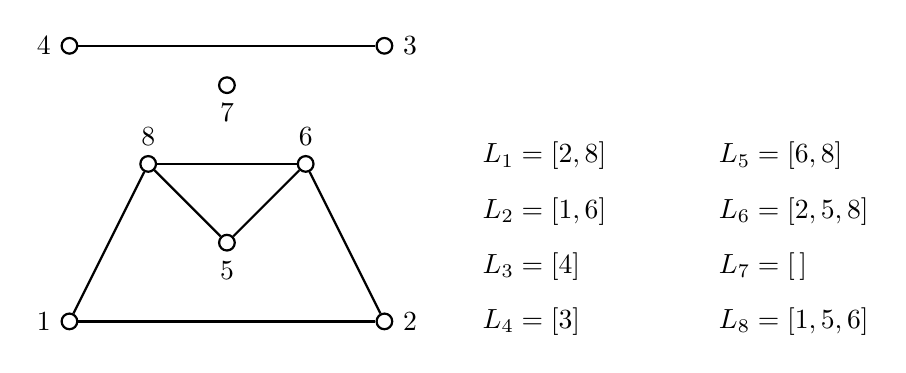
\begin{tikzpicture}
[nodedecorate/.style={shape=circle,inner sep=2pt,draw,thick},%
  linedecorate/.style={-,thick}]
%% nodes or vertices
\foreach \nodename/\x/\y/\direction/\navigate in {
  1/0/0/left/west, 2/4/0/right/east, 3/4/3.5/right/east,
  4/0/3.5/left/west, 5/2/1/below/south, 6/3/2/above/north,
  7/2/3/below/south, 8/1/2/above/north} {
  \node (\nodename) at (\x,\y) [nodedecorate] {};
  \node [\direction] at (\nodename.\navigate) {$\nodename$};
}
%% adjacency lists
\node (L1) at (5,2.1) [] {};
\node [right] at (L1.east) {$L_1 = [2,8]$};
\node (L2) at (5,1.4) [] {};
\node [right] at (L2.east) {$L_2 = [1,6]$};
\node (L3) at (5,0.7) [] {};
\node [right] at (L3.east) {$L_3 = [4]$};
\node (L4) at (5,0) [] {};
\node [right] at (L4.east) {$L_4 = [3]$};
\node (L5) at (8,2.1) [] {};
\node [right] at (L5.east) {$L_5 = [6,8]$};
\node (L6) at (8,1.4) [] {};
\node [right] at (L6.east) {$L_6 = [2,5,8]$};
\node (L7) at (8,0.7) [] {};
\node [right] at (L7.east) {$L_7 = [\,]$};
\node (L8) at (8,0) [] {};
\node [right] at (L8.east) {$L_8 = [1,5,6]$};
%% edges or lines
\path
\foreach \startnode/\endnode in {1/2, 1/8, 2/6, 3/4, 5/6, 5/8, 6/8} {
  (\startnode) edge[linedecorate] node {} (\endnode)
};
\end{tikzpicture}
\caption{A graph and its adjacency lists.}
\label{fig:graph_algorithms:graph_adjacency_lists}
\end{figure}

We can categorize a graph $G = (V, E)$ as \emph{dense} or
\emph{sparse} based upon its size. A dense graph\index{dense graph}
has size $|E|$ that is close to $|V|^2$, i.e.
$|E| = \Omega\big(|V|^2\big)$, in which case it is feasible to
represent $G$ as an adjacency matrix. The size of a sparse
graph\index{sparse graph} is much less than $|V|^2$, i.e.
$|E| = \Omega\big(|V|\big)$, which renders the adjacency matrix
representation as unsuitable. For a sparse graph, an adjacency list
representation can require less storage space than an adjacency matrix
representation of the same graph.


%%%%%%%%%%%%%%%%%%%%%%%%%%%%%%%%%%%%%%%%%%%%%%%%%%%%%%%%%%%%%%%%%%%%%%%%%%%

\subsection{The {\tt graph6} format}
\label{sec:graph_algorithms:graph6_format}

The graph formats {\tt graph6} and {\tt sparse6} were developed by Brendan
McKay~\cite{McKay2010} at The Australian National University as a
compact way to represent graphs. These two formats use bit vectors and
printable characters of the American Standard Code for Information
Interchange~(ASCII) encoding scheme. The 64 printable ASCII characters
used in {\tt graph6} and {\tt sparse6} are those ASCII characters with decimal
codes from 63 to 126, inclusive, as shown in
Table~\ref{tab:graph_algorithms:graph6_sparse6_ASCII_printable_characters}.
This section shall only cover the {\tt graph6} format. For full
specification on both of the {\tt graph6} and {\tt sparse6} formats, see
McKay~\cite{McKay2010}.

\begin{table}[!htbp]
\centering
\begin{tabular}{ccc|ccc} \hline
binary         & decimal   & glyph    & binary & decimal & glyph \\\hline
\verb!0111111! & \verb!63! & \verb!?! & \verb!1011111! & \verb!95!  & \verb!_! \\
\verb!1000000! & \verb!64! & \verb!@! & \verb!1100000! & \verb!96!  & \verb!`! \\
\verb!1000001! & \verb!65! & \verb!A! & \verb!1100001! & \verb!97!  & \verb!a! \\
\verb!1000010! & \verb!66! & \verb!B! & \verb!1100010! & \verb!98!  & \verb!b! \\
\verb!1000011! & \verb!67! & \verb!C! & \verb!1100011! & \verb!99!  & \verb!c! \\
\verb!1000100! & \verb!68! & \verb!D! & \verb!1100100! & \verb!100! & \verb!d! \\
\verb!1000101! & \verb!69! & \verb!E! & \verb!1100101! & \verb!101! & \verb!e! \\
\verb!1000110! & \verb!70! & \verb!F! & \verb!1100110! & \verb!102! & \verb!f! \\
\verb!1000111! & \verb!71! & \verb!G! & \verb!1100111! & \verb!103! & \verb!g! \\
\verb!1001000! & \verb!72! & \verb!H! & \verb!1101000! & \verb!104! & \verb!h! \\
\verb!1001001! & \verb!73! & \verb!I! & \verb!1101001! & \verb!105! & \verb!i! \\
\verb!1001010! & \verb!74! & \verb!J! & \verb!1101010! & \verb!106! & \verb!j! \\
\verb!1001011! & \verb!75! & \verb!K! & \verb!1101011! & \verb!107! & \verb!k! \\
\verb!1001100! & \verb!76! & \verb!L! & \verb!1101100! & \verb!108! & \verb!l! \\
\verb!1001101! & \verb!77! & \verb!M! & \verb!1101101! & \verb!109! & \verb!m! \\
\verb!1001110! & \verb!78! & \verb!N! & \verb!1101110! & \verb!110! & \verb!n! \\
\verb!1001111! & \verb!79! & \verb!O! & \verb!1101111! & \verb!111! & \verb!o! \\
\verb!1010000! & \verb!80! & \verb!P! & \verb!1110000! & \verb!112! & \verb!p! \\
\verb!1010001! & \verb!81! & \verb!Q! & \verb!1110001! & \verb!113! & \verb!q! \\
\verb!1010010! & \verb!82! & \verb!R! & \verb!1110010! & \verb!114! & \verb!r! \\
\verb!1010011! & \verb!83! & \verb!S! & \verb!1110011! & \verb!115! & \verb!s! \\
\verb!1010100! & \verb!84! & \verb!T! & \verb!1110100! & \verb!116! & \verb!t! \\
\verb!1010101! & \verb!85! & \verb!U! & \verb!1110101! & \verb!117! & \verb!u! \\
\verb!1010110! & \verb!86! & \verb!V! & \verb!1110110! & \verb!118! & \verb!v! \\
\verb!1010111! & \verb!87! & \verb!W! & \verb!1110111! & \verb!119! & \verb!w! \\
\verb!1011000! & \verb!88! & \verb!X! & \verb!1111000! & \verb!120! & \verb!x! \\
\verb!1011001! & \verb!89! & \verb!Y! & \verb!1111001! & \verb!121! & \verb!y! \\
\verb!1011010! & \verb!90! & \verb!Z! & \verb!1111010! & \verb!122! & \verb!z! \\
\verb!1011011! & \verb!91! & \verb![! & \verb!1111011! & \verb!123! & \verb!{! \\
\verb!1011100! & \verb!92! & \verb!\! & \verb!1111100! & \verb!124! & \verb!|! \\
\verb!1011101! & \verb!93! & \verb!]! & \verb!1111101! & \verb!125! & \verb!}! \\
\verb!1011110! & \verb!94! & \verb!^! & \verb!1111110! & \verb!126! & \verb!~! \\\hline
\end{tabular}
\caption{ASCII printable characters used by graph6 and sparse6.}
\label{tab:graph_algorithms:graph6_sparse6_ASCII_printable_characters}
\end{table}


%%%%%%%%%%%%%%%%%%%%%%%%%%%%%%%%%%%%%%%%%%%%%%%%%%%%%%%%%%%%%%%%%%%%%%%%%%%

\subsubsection{Bit vectors}

Before discussing how {\tt graph6} and {\tt sparse6} represent graphs using
printable ASCII characters, we first present encoding schemes used by
these two formats. A \emph{bit vector} is, as its name suggests, a
vector whose elements are 1's and 0's. It can be represented as a list
of bits, e.g. \verb!E! can be represented as the ASCII bit vector
$[\texttt{1}, \texttt{0}, \texttt{0}, \texttt{0}, \texttt{1},
  \texttt{0}, \texttt{1}]$. For brevity, we write a bit vector in a
compact form such as \texttt{1000101}. The \emph{length} of a bit
vector is its number of bits. The \emph{most significant bit}
of a bit vector $v$ is the bit position with the largest value among
all the bit positions in $v$. Similarly, the
\emph{least significant bit} is the bit position in $v$ having the
least value among all the bit positions in $v$. The least significant
bit of $v$ is usually called the parity bit because when $v$
interpreted as an integer the parity bit determines whether the
integer is even or odd. Reading \texttt{1000101} from left to right,
the first bit \texttt{1} is the most significant bit, followed by the
second bit \texttt{0} which is the second most significant bit, and so
on all the way down to the seventh bit \texttt{1} which is the least
significant bit.

The order in which we process the bits of a bit vector is referred to
as \emph{endianness}. Processing $v$ in \emph{big-endian} order means
\index{big-endian order}
\index{endianness}
that we first process the most significant bit of $v$, followed by the
second most significant bit, and so on all the way down to the least
significant bit of $v$. \emph{Little-endian} order means that we first
process the least significant bit, followed by the second least
significant bit, and so on all the way up to the most significant
bit. In big-endian order, the ASCII binary representation of
\texttt{E} is written \texttt{1000101}~(see
Table~\ref{tab:graph_algorithms:big_endian_ASCII_binary_E}), while
the little-ending order is written \texttt{1010001}~(see
Table~\ref{tab:graph_algorithms:little_endian_ASCII_binary_E}). To
determine the integer representation of a bit vector, multiply each
bit value by its corresponding position value, then add up all the
results. In general, if the bit vector $v = b_1 b_2 \cdots b_k$ is the
big-endian binary representation of a positive integer, then the
integer representation of $v$ is
%
\begin{equation}
\label{eq:graph_algorithms:big_endian_binary_to_integer}
\sum_{i=1}^k 2^{k-i} b_i
=
2^{k-1} b_1 + 2^{k-2} b_2 + 2^{k-3} b_3 + \cdots + 2^0 b_k.
\end{equation}

\begin{table}[!htbp]
\centering
\begin{tabular}{l|ccccccc} \hline
position       & 1          & 2          & 3          & 4          & 5          & 6          & 7 \\
bit value      & \texttt{1} & \texttt{0} & \texttt{0} & \texttt{0} & \texttt{1} & \texttt{0} & \texttt{1} \\
position value & $2^6$      & $2^5$      & $2^4$      & $2^3$      & $2^2$      & $2^1$      & $2^0$ \\\hline
\end{tabular}
\caption{Big-endian order of the ASCII binary code of \texttt{E}.}
\label{tab:graph_algorithms:big_endian_ASCII_binary_E}
\end{table}

\begin{table}[!htbp]
\centering
\begin{tabular}{l|ccccccc} \hline
position       & 1          & 2          & 3          & 4          & 5          & 6          & 7 \\
bit value      & \texttt{1} & \texttt{0} & \texttt{1} & \texttt{0} & \texttt{0} & \texttt{0} & \texttt{1} \\
position value & $2^0$      & $2^1$      & $2^2$      & $2^3$      & $2^4$      & $2^5$      & $2^6$ \\\hline
\end{tabular}
\caption{Little-endian order of the ASCII binary code of \texttt{E}.}
\label{tab:graph_algorithms:little_endian_ASCII_binary_E}
\end{table}

In {\tt graph6} and {\tt sparse6} formats, the length of a bit vector must be a
multiple of 6. Suppose $v$ is a bit vector of length $k$ such that
$6 \nmid k$. To transform $v$ into a bit vector having length a
multiple of 6, let $r = k \mod 6$ be the remainder upon dividing $k$
by 6, and pad $6 - r$ zeros to the right of $v$.

Suppose $v = b_1 b_2 \cdots b_k$ is a bit vector of length $k$, where
$6 \;|\; k$. We split $v$ into $k/6$ bit vectors $v_i$, each of length
6. For $0 \leq i \leq k/6$, the $i$-th bit vector is given by
\[
v_i
=
b_{6i-5} b_{6i-4} b_{6i-3} b_{6i-2} b_{6i-1} b_{6i}.
\]
Consider each $v_i$ as the big-endian binary representation of a
positive
integer. Use~(\ref{eq:graph_algorithms:big_endian_binary_to_integer})
to obtain the integer representation $N_i$ of each $v_i$. Then add 63
to each $N_i$ to obtain $N_i'$ and store $N_i'$ in one byte of
memory. That is, each $N_i'$ can be represented as a bit vector of
length $8$. Thus the required number of bytes to store $v$ is
$\lceil k/6 \rceil$. Let $B_i$ be the byte representation of $N_i'$ so
that
%
\begin{equation}
\label{eq:graph_algorithms:byte_representation_bit_vector}
R(v)
=
B_1 B_2 \cdots B_{\lceil k/6 \rceil}
\end{equation}
%
denotes the representation of $v$ as a sequence of $\lceil k/6 \rceil$
bytes.

We now discuss how to encode an integer $n$ in the range
$0 \leq n \leq 2^{36} - 1$
using~(\ref{eq:graph_algorithms:byte_representation_bit_vector}) and
denote such an encoding of $n$ as $N(n)$. Let $v$ be the big-endian
binary representation of $n$. Then $N(n)$ is given by
%
\begin{equation}
\label{eq:graph_algorithms:graph6_sparse6_graph_orders}
N(n)
=
\begin{cases}
n + 63, & \text{if $0 \leq n \leq 62$}, \\
126 \, R(v), & \text{if $63 \leq n \leq 258047$}, \\
126 \, 126 \, R(v), & \text{if $258048 \leq n \leq 2^{36}-1$}.
\end{cases}
\end{equation}
%% If $0 \leq n \leq 62$, then
%% we write $N(n) = n + 63$. If $63 \leq n \leq 258047$, let $v$ be the
%% big-endian binary representation of $n$ and write
%% $N(n) = 126 \, R(v)$. Finally, if $258048 \leq n \leq 2^{36} - 1$,
%% again we let $v$ be the big-endian binary representation of $n$ and
%% write $N(n) = 126 \, 126 \, R(v)$.
Note that $n + 63$ requires one byte of storage memory, while
$126 \, R(v)$ and $126 \, 126 \, R(v)$ require 4 and 8 bytes,
respectively.


%%%%%%%%%%%%%%%%%%%%%%%%%%%%%%%%%%%%%%%%%%%%%%%%%%%%%%%%%%%%%%%%%%%%%%%%%%%

\subsubsection{The {\tt graph6} format}
\index{graph6}

The {\tt graph6} format is used to represent simple, undirected graphs of
order from $0$ to $2^{36} - 1$, inclusive. Let $G$ be a simple,
undirected graph of order $0 \leq n \leq 2^{36} - 1$. If $n = 0$, then
$G$ is represented in {\tt graph6} format as ``\verb!?!''. Suppose $n >
0$. Let $M = [a_{ij}]$ be the adjacency matrix of $G$. Consider the
upper triangle of $M$, excluding the main diagonal, and write that
upper triangle as the bit vector
\[
v
=
\underbrace{a_{0,1}}_{c_1}
\underbrace{a_{0,2} a_{1,2}}_{c_2}
\underbrace{a_{0,3} a_{1,3} a_{2,3}}_{c_3} \cdots
\underbrace{a_{0,i} a_{1,i} \cdots a_{i-1,i}}_{c_i} \cdots
\underbrace{a_{0,n} a_{1,n} \cdots a_{n-1,n}}_{c_n}
\]
where $c_i$ denotes the entries $a_{0,i} a_{1,i} \cdots a_{i-1,i}$ in
column $i$ of $M$. Then the {\tt graph6} representation of $G$ is
$N(n) R(v)$, where $R(v)$ and $N(n)$ are as
in~(\ref{eq:graph_algorithms:byte_representation_bit_vector})
and~(\ref{eq:graph_algorithms:graph6_sparse6_graph_orders}),
respectively. That is, $N(n)$ encodes the order of $G$ and $R(v)$
encodes the edges of $G$.


%%%%%%%%%%%%%%%%%%%%%%%%%%%%%%%%%%%%%%%%%%%%%%%%%%%%%%%%%%%%%%%%%%%%%%%%%%%

\section{Graph searching}
\label{sec:graph_algorithms:graph_searching}

This section discusses two fundamental algorithms for graph traversal:
breadth-first search and depth-first search. The word ``search'' used
in describing these two algorithms is rather misleading. It would be
more accurate to describe them as algorithms for constructing trees
using the adjacency information of a given graph. However, the names
``breadth-first search'' and ``depth-first search'' are entrenched in
literature on graph theory and computer science. From hereon, we use
these two names as given above, bearing in mind their intended
purposes.


%%%%%%%%%%%%%%%%%%%%%%%%%%%%%%%%%%%%%%%%%%%%%%%%%%%%%%%%%%%%%%%%%%%%%%%%%%%

\subsection{Breadth-first search}

Breadth-first search (BFS) is a strategy for running through the
vertices of a graph. It was presented by Moore~\cite{Moore1959} in
1959 within the context of traversing mazes. Lee~\cite{Lee1961}
independently discovered the same algorithm in 1961 in his work on
routing wires on circuit boards.

The basic BFS algorithm can be described as follows. Starting from a
given vertex $v$ of a graph $G$, we first explore the neighborhood of
$v$ by visiting all vertices that are adjacent to $v$. We then apply
the same strategy to each of the neighbors of $v$. The strategy of
exploring the neighborhood of a vertex is applied to all vertices of
$G$. The result is a tree rooted at $v$ and this tree is a subgraph of
$G$. Algorithm~\ref{alg:graph_algorithms:breadth_first_search_template}
presents a general template for the BFS strategy. The tree resulting
from the BFS algorithm is called a \emph{breadth-first search tree}.
\index{BFS}
\index{breadth-first search}

\begin{algorithm}[!htpb]
\dontprintsemicolon  % no semicolon at end of pseudocode statements
%% data section
\SetKwInOut{Input}{Input}
\SetKwInOut{Output}{Output}
%% input/output
\Input{A directed or undirected graph $G = (V, E)$ of order $n > 0$. A
  vertex $s$ from which to start the search. The vertices are numbered
  from $1$ to  $n = |V|$, i.e. $V = \{1, 2, \dots, n\}$.}
\Output{A list $D$ of distances of all vertices from $s$. A tree $T$
  rooted at $s$.}
\BlankLine
$Q \leftarrow [s]$~\nllabel{alg:BFS:initialize_queue_visit_nodes} \tcc*[f]{queue of nodes to visit}\;
$D \leftarrow [\infty, \infty, \dots, \infty]$ \tcc*[f]{$n$ copies of $\infty$}\;
$D[s] \leftarrow 0$\;
$T \leftarrow [\,]$~\nllabel{alg:BFS:initialize_empty_tree}\;
\While{$\length(Q) > 0$~\nllabel{alg:BFS:while_loop:non_empty_queue}}{
  $v \leftarrow \dequeue(Q)$\;
  \For{\emph{each} $w \in \adj(v)$~\nllabel{alg:BFS:explore_neighborhood}}{
    \If{$D[w] = \infty$~\nllabel{alg:BFS:marking_vertex_as_visited}}{
      $D[w] \leftarrow D[v] + 1$\;
      $\enqueue(Q, w)$\;
      $\append(T, vw)$~\nllabel{alg:BFS:while_loop:append_to_tree}\;
    }
  }
}
\Return $(D, T)$\;
\caption{A general breadth-first search template.}
\label{alg:graph_algorithms:breadth_first_search_template}
\end{algorithm}

The breadth-first search algorithm makes use of a special type of list
called a \emph{queue}. This is analogous to a queue of people waiting
in line to be served. A person may enter the queue by joining the rear
of the queue. The person who is in the queue the longest amount of
time is served first, followed by the person who has waited the second
longest time, and so on. Formally, a queue $Q$ is a list of
elements. At any time, we only have access to the first element of
$Q$, known as the \emph{front} or \emph{start} of the queue. We insert
a new element into $Q$ by appending the new element to the \emph{rear}
or \emph{end} of the queue. The operation of removing the front of $Q$
is referred to as \emph{dequeue}, while the operation of appending to
the rear of $Q$ is called \emph{enqueue}. That is, a queue implements
a first-in first-out~(FIFO) protocol for adding and moving
elements. As with lists, the \emph{length} of a queue is its total
number of elements.

\begin{figure}[!htbp]
\centering
\subfigure[]{
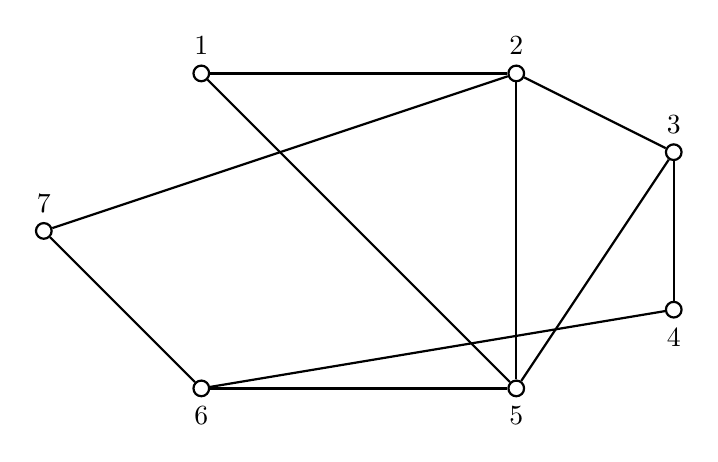
\begin{tikzpicture}
[nodedecorate/.style={shape=circle,inner sep=2pt,draw,thick},%
  linedecorate/.style={-,thick}]
%% nodes or vertices
\foreach \nodename/\x/\y/\direction/\navigate in {2/4/4/above/north,
  1/0/4/above/north, 3/6/3/above/north, 4/6/1/below/south,
  5/4/0/below/south, 7/-2/2/above/north, 6/0/0/below/south} {
  \node (\nodename) at (\x,\y) [nodedecorate] {};
  \node [\direction] at (\nodename.\navigate) {$\nodename$};
}
%% edges or lines
\path
\foreach \startnode/\endnode in {1/2, 1/5, 2/3, 2/5, 2/7, 3/4, 3/5,
  4/6, 5/6, 6/7} {
  (\startnode) edge[linedecorate] node {} (\endnode)
};
\end{tikzpicture}
}
%%
\qquad
\subfigure[]{
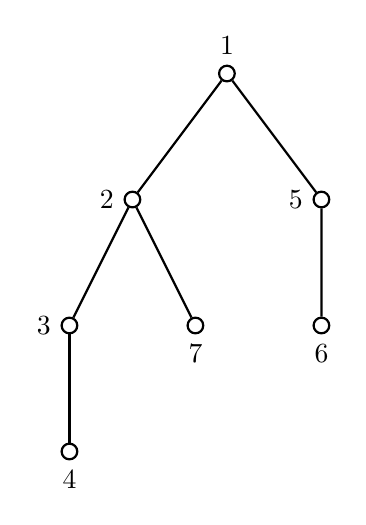
\begin{tikzpicture}
[nodedecorate/.style={shape=circle,inner sep=2pt,draw,thick},%
  linedecorate/.style={-,thick},%
  scale=1.6]
%% nodes or vertices
\foreach \nodename/\x/\y/\direction/\navigate in {4/0/0/below/south,
  3/0/1/left/west, 7/1/1/below/south, 6/2/1/below/south,
  2/0.5/2/left/west, 5/2/2/left/west, 1/1.25/3/above/north} {
  \node (\nodename) at (\x,\y) [nodedecorate] {};
  \node [\direction] at (\nodename.\navigate) {$\nodename$};
}
%% edges or lines
\path
\foreach \startnode/\endnode in {1/2, 1/5, 2/3, 2/7, 3/4, 5/6} {
  (\startnode) edge[linedecorate] node {} (\endnode)
};
\end{tikzpicture}
}
%%
%%
\subfigure[]{
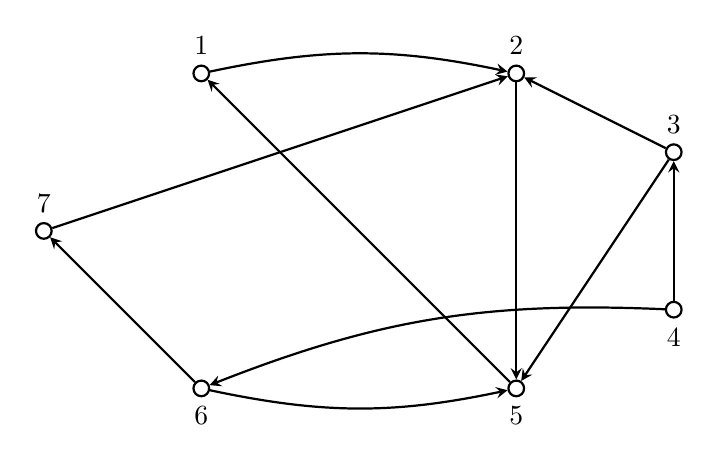
\begin{tikzpicture}
[nodedecorate/.style={shape=circle,inner sep=2pt,draw,thick},%
  arrowdecorate/.style={->,>=stealth,thick}]
%% nodes or vertices
\foreach \nodename/\x/\y/\direction/\navigate in {2/4/4/above/north,
  1/0/4/above/north, 3/6/3/above/north, 4/6/1/below/south,
  5/4/0/below/south, 7/-2/2/above/north, 6/0/0/below/south} {
  \node (\nodename) at (\x,\y) [nodedecorate] {};
  \node [\direction] at (\nodename.\navigate) {$\nodename$};
}
%% edges or lines
\path
\foreach \startnode/\endnode in {2/5, 3/2, 3/5, 4/3, 5/1, 6/7, 7/2} {
  (\startnode) edge[arrowdecorate] node {} (\endnode)
}
\foreach \startnode/\endnode/\benddirection/\angle in {
  1/2/bend left/12, 4/6/bend right/12, 6/5/bend right/12} {
  (\startnode) edge[arrowdecorate,\benddirection=\angle] node {} (\endnode)
};
\end{tikzpicture}
}
%%
\qquad
\subfigure[]{
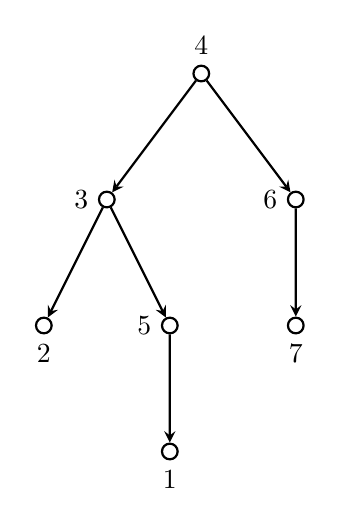
\begin{tikzpicture}
[nodedecorate/.style={shape=circle,inner sep=2pt,draw,thick},%
  arrowdecorate/.style={->,>=stealth,thick},
  scale=1.6]
%% nodes or vertices
\foreach \nodename/\x/\y/\direction/\navigate in {2/0/1/below/south,
  1/1/0/below/south, 5/1/1/left/west, 7/2/1/below/south,
  6/2/2/left/west, 3/0.5/2/left/west, 4/1.25/3/above/north} {
  \node (\nodename) at (\x,\y) [nodedecorate] {};
  \node [\direction] at (\nodename.\navigate) {$\nodename$};
}
%% edges or lines
\path
\foreach \startnode/\endnode in {4/3, 4/6, 3/2, 3/5, 6/7, 5/1} {
  (\startnode) edge[arrowdecorate] node {} (\endnode)
};
\end{tikzpicture}
}
\caption{Breadth-first search trees for undirected and directed graphs.}
\label{fig:graph_algorithms:breadth_first_search_undirected}
\end{figure}

Note that the BFS
Algorithm~\ref{alg:graph_algorithms:breadth_first_search_template}
works on both undirected and directed graphs. For an undirected graph,
line~\ref{alg:BFS:explore_neighborhood} means that we explore all
the neighbors of vertex $v$, i.e. the set $\adj(v)$ of vertices
adjacent to $v$. In the case of a digraph, we replace
``$w \in \adj(v)$'' on line~\ref{alg:BFS:explore_neighborhood} with
``$w \in \oadj(v)$'' because we only want to explore all vertices that
are out-neighbors of $v$. The algorithm returns two lists $D$ and
$T$. The list $T$ contains a subset of edges in $E(G)$ that make up a
tree rooted at the given start vertex $s$. As trees are connected
graphs without cycles, we may take the vertices comprising the edges
of $T$ to be the vertex set of the tree. It is clear that $T$
represents a tree by means of a list of edges, which allows us to
identify the tree under consideration as the edge list $T$. The list
$D$ has the same number of elements as the order of $G = (V, E)$,
i.e. $\length(D) = |V|$. The $i$-th element $D[i]$ counts the number
of edges in $T$ between the vertices $s$ and $v_i$. In other words,
$D[i]$ is the length of the $s$-$v_i$ path in $T$. It can be shown
that $D[i] = \infty$ if and only if $G$ is disconnected. After one
application of
Algorithm~\ref{alg:graph_algorithms:breadth_first_search_template}, it
may happen that $D[i] = \infty$ for at least one vertex
$v_i \in V$. To traverse those vertices that are unreachable from $s$,
again we apply
Algorithm~\ref{alg:graph_algorithms:breadth_first_search_template} on
$G$ with starting vertex $v_i$. Repeat this algorithm as often as
necessary until all vertices of $G$ are visited. The result may be a
tree that contains all the vertices of $G$ or a collection of trees,
each of which contains a subset of $V(G)$.
Figure~\ref{fig:graph_algorithms:breadth_first_search_undirected}
presents BFS trees resulting from applying
Algorithm~\ref{alg:graph_algorithms:breadth_first_search_template} on
an undirected graph and a digraph.

\begin{theorem}
\label{thm:graph_algorithms:BFS:worst_case_time_complexity}
The worst-case time complexity of
Algorithm~\ref{alg:graph_algorithms:breadth_first_search_template} is
$O(|V| + |E|)$.
\end{theorem}

\begin{proof}
Without loss of generality, we can assume that $G = (V, E)$ is
connected. The initialization steps in
lines~\ref{alg:BFS:initialize_queue_visit_nodes}
to~\ref{alg:BFS:initialize_empty_tree} take $O(|V|)$ time. After
initialization, all but one vertex are labelled
$\infty$. Line~\ref{alg:BFS:marking_vertex_as_visited} ensures that
each vertex is enqueued at most once and hence dequeued at most
once. Each of enqueuing and dequeuing takes constant time. The total
time devoted to queue operations is $O(|V|)$. The adjacency list of a
vertex is scanned after dequeuing that vertex, so each adjacency list
is scanned at most once. Summing the lengths of the adjacency lists,
we have $\Theta(|E|)$ and therefore we require $O(|E|)$ time to scan
the adjacency lists. After the adjacency list of a vertex is scanned,
at most $k$ edges are added to the list $T$, where $k$ is the length
of the adjacency list under consideration. Like queue operations,
appending to a list takes constant time, hence we require $O(|E|)$
time to build the list $T$. Therefore, BFS runs in $O(|V| + |E|)$
time.
\end{proof}

\begin{theorem}
\label{thm:graph_algorithms:BFS:list_D_length_shortest_paths}
For the list $D$ resulting from
Algorithm~\ref{alg:graph_algorithms:breadth_first_search_template},
let $s$ be a starting vertex and let $v$ be a vertex such that
$D[v] \neq \infty$. Then $D[v]$ is the length of any shortest path
from $s$ to $v$.
\end{theorem}

\begin{proof}
It is clear that $D[v] = \infty$ if and only if there are no paths
from $s$ to $v$. Let $v$ be a vertex such that $D[v] \neq \infty$. As
$v$ can be reached from $s$ by a path of length $D[v]$, the length
$d(s,v)$ of any shortest $s$-$v$ path satisfies $d(s,v) \leq
D[v]$. Use induction on $d(s,v)$ to show that equality holds. For the
base case $s = v$, we have $d(s,v) = D[v] = 0$ since the trivial path
has length zero. Assume for induction that if $d(s,v) = k$, then
$d(s,v) = D[v]$.
%% We need to show that if $d(s,u)$ is the length of any
%% shortest $s$-$u$ path, then $d(s,u) = D[u]$.
Let $d(s,u) = k + 1$ with the corresponding shortest $s$-$u$ path
being $(s, v_1, v_2, \dots, v_k, u)$. Then by our induction
hypothesis, $(s, v_1, v_2, \dots, v_k)$ is a shortest path from $s$ to
$v_k$ of length $d(s, v_k) = D[v_k] = k$. In other words, $D[v_k] <
D[u]$ and the while loop spanning
lines~\ref{alg:BFS:while_loop:non_empty_queue}
to~\ref{alg:BFS:while_loop:append_to_tree} processes $v_k$ before
processing $u$. The graph under consideration has the edge $v_k
u$. When examining the adjacency list of $v_k$, BFS reaches $u$~(if
$u$ is not reached earlier) and so $D[u] \leq k + 1$. Hence,
$D[u] = k + 1$ and therefore $d(s,u) = D[u] = k + 1$.
\end{proof}

%% Another version of
%% Algorithm~\ref{alg:graph_algorithms:breadth_first_search} is where you
%% are searching the graph for a vertex (or edge) satisfying a certain
%% property $P$. In that situation, you simply quit at the step where you
%% increment the counter, i.e. line~7 in
%% Algorithm~\ref{alg:graph_algorithms:breadth_first_search}. Other
%% variations are also possible as well.

%% For the example of the graph in
%% Figure~\ref{fig:introduction:types_of_walks}, the list of distances
%% from vertex \verb!a! to any other vertex is
%% %
%% \begin{center}
%% \fontsize{9pt}{9pt}
%% \selectfont
%% \tt
%% \begin{lstlisting}
%% [['a', 0], ['b', 1], ['c', 2], ['d', 3], ['e', 1], ['f', 2], ['g', 2]]
%% \end{lstlisting}
%% \end{center}
%% %
%% To create this list,
%% %
%% \begin{itemize}
%% \item
%% Start at \verb!a! and compute the distance from \verb!a! to itself.

%% \item
%% Move to each neighbor of \verb!a!, namely \verb!b! and \verb!e!, and
%% compute the distance from \verb!a! to each of them.

%% \item
%% Move to each ``unseen'' neighbor of \verb!b!, namely just \verb!c!,
%% and compute the distance from \verb!a! to it.

%% \item
%% Move to each ``unseen'' neighbor of \verb!e!, namely just \verb!f!,
%% and compute the distance from \verb!a! to it.

%% \item
%% Move to each ``unseen'' neighbor of \verb!c!, namely just \verb!d!,
%% and compute the distance from \verb!a! to it.

%% \item
%% Move to each ``unseen'' neighbor of \verb!f!, namely just \verb!g!,
%% and compute the distance from \verb!a! to it.
%% \end{itemize}

%% As an example, here is some Sage code which implements BFS to compute
%% the list distances from a given vertex.
%% %
%% \begin{center}
%% \fontsize{9pt}{9pt}
%% \selectfont
%% \tt
%% \begin{lstlisting}
%% def graph_distance(G, v0):
%%     """
%%     Breadth first search algorithm to find the
%%     distance from a fixed vertex $v_0$ to any
%%     other vertex.

%%     INPUT:
%%         G - a connected graph
%%         v0 - a vertex

%%     OUTPUT:
%%         D - a list of distances to
%%             every other vertex

%%     EXAMPLES:
%%         sage: G = Graph({1: [2, 4], 2: [1, 4], 3: [2, 6],
%%                          4: [1, 3], 5: [4, 2], 6: [3, 1]})
%%         sage: v0 = 1
%%         sage: graph_distance(G,v0)
%%         [[1, 0], [2, 1], [3, 2], [4, 1], [5, 2], [6, 1]]
%%         sage: G = Graph({"a": ["b", "e"], "b": ["c", "e"], \
%%          "c": ["d", "e"], "d": ["f"], "e": ["f"], "f": ["g"], "g":["b"]})
%%         sage: v0 = "a"
%%         sage: graph_distance(G, v0)
%%         [['a', 0], ['b', 1], ['c', 2], ['d', 3], ['e', 1],
%%          ['f', 2], ['g', 2]]
%%         sage: G = Graph({1: [2,3], 2: [1, 3], 3: [2], 4: [5], 5: [6], 6: [5]})
%%         sage: v0 = 1
%%         sage: graph_distance(G, v0) # note G is disconnected
%%         [[1, 0], [2, 1], [3, 1]]
%%     """
%%     V = G.vertices()
%%     Q = [v0]
%%     T = []
%%     D = []
%%     while Q<>[] and T<>V:
%%         for v in Q:
%%             if not(v in T):
%%                 D.append([v,G.distance(v0,v)])
%%             if v in Q:
%%                 Q.remove(v)
%%             T.append(v)
%%             T = list(Set(T))
%%             Q = Q+[x for x in G.neighbors(v) if not(x in T+Q)]
%%             if T == V:
%%                 break
%%     D.sort()
%%     print Q, T
%%     return D
%% \end{lstlisting}
%% \end{center}
%% %
%% \begin{exercise}
%% Using Sage's \verb!shortest_path! method, can you modify the above
%% function to return a list of shortest paths from $v_0$ to any other
%% vertex?
%% \end{exercise}


%%%%%%%%%%%%%%%%%%%%%%%%%%%%%%%%%%%%%%%%%%%%%%%%%%%%%%%%%%%%%%%%%%%%%%%%%%%

\subsection{Depth-first search}

\begin{quote}
\includegraphics[scale=0.5]{image/depth-first-search} \\
\noindent
--- Randall Munroe\index{Munroe, Randall}, xkcd,
\url{http://xkcd.com/761/}
\end{quote}

\noindent
A depth-first search~(DFS) is a graph traversal strategy similar to
breadth-first search. Both BFS and DFS differ in how they explore each
vertex. Whereas BFS explores the neighborhood of a vertex $v$ before
moving on to explore the neighborhoods of the neighbors, DFS explores
as deep as possible a path starting at $v$. One can think of BFS as
exploring the immediate surrounding, while DFS prefers to see what is
on the other side of the hill. In the 19th century,
Lucas~\cite{Lucas1882.1894} and Tarry~\cite{Tarry1895} investigated
DFS as a strategy for traversing mazes. Fundamental properties of DFS
were discovered in the early 1970s by Hopcroft and
Tarjan~\cite{HopcroftTarjan1973,Tarjan1972}.

To get an intuitive appreciation for DFS, suppose we have an
$8 \times 8$ chessboard in front of us. We place a single knight
piece on a fixed square of the board. Our objective is to find a
sequence of knight moves that visits each and every square exactly
once, while obeying the rules of chess that govern the movement of the
knight piece. Such a sequence of moves, if one exists, is called a
\emph{knight's tour}. How do we find such a tour? We could make one
knight move after another, recording each move to ensure that we do
not step on a square that is already visited, until we could not make
any more moves. Acknowledging defeat when encountering a dead end, it
might make sense to \emph{backtrack} a few moves and try again, hoping
we would not get stuck. If we fail again, we try backtracking a few
more moves and traverse yet another path, hoping to make further
progress. Repeat this strategy until a tour is found or until we have
exhausted all possible moves. The above strategy for finding a
knight's tour is an example of depth-first search, sometimes called
\emph{backtracking}.
\index{backtracking}
\index{knight's tour}

\begin{algorithm}[!htpb]
\dontprintsemicolon  % no semicolon at end of pseudocode statements
%% data section
\SetKwInOut{Input}{Input}
\SetKwInOut{Output}{Output}
%% input/output
\Input{A directed or undirected graph $G = (V, E)$ of order $n > 0$. A
  vertex $s$ from which to start the search. The vertices are numbered
  from $1$ to  $n = |V|$, i.e. $V = \{1, 2, \dots, n\}$.}
\Output{A list $D$ of distances of all vertices from $s$. A tree $T$
  rooted at $s$.}
\BlankLine
$S \leftarrow [s]$ \tcc*[f]{stack of nodes to visit}\;
$D \leftarrow [\infty, \infty, \dots, \infty]$ \tcc*[f]{$n$ copies of $\infty$}\;
$D[s] \leftarrow 0$\;
$T \leftarrow [\,]$\;
\While{$\length(S) > 0$~\nllabel{alg:DFS:while_loop_tests_non_empty_stack}}{
  $v \leftarrow \pop(S)$\;
  \For{\emph{each} $w \in \adj(v)$~\nllabel{alg:DFS:for_loop_visit_neighbors}}{
    \If{$D[w] = \infty$~\nllabel{alg:DFS:if_test_unvisited_neighbors}}{
      $D[w] \leftarrow D[v] + 1$\;
      $\push(S, w)$\;
      $\append(T, vw)$\;
    }
  }
}
\Return $(D, T)$\;
\caption{A general depth-first search template.}
\label{alg:graph_algorithms:depth_first_search_template}
\end{algorithm}

Algorithm~\ref{alg:graph_algorithms:depth_first_search_template}
formalizes the above description of depth-first search. The tree
resulting from applying DFS on a graph is called a
\emph{depth-first search tree}. The general structure of this
algorithm bears close resemblance to
Algorithm~\ref{alg:graph_algorithms:breadth_first_search_template}. A
significant difference is that instead of using a queue to structure
and organize vertices to be visited, DFS uses another special type of
list called a \emph{stack}. To understand how elements of a stack are
organized, we use the analogy of a stack of cards. A new card is added
to the stack by placing it on top of the stack. Any time we want to
remove a card, we are only allowed to remove the top-most card that is
on the top of the stack. A list $L = [a_1, a_2, \dots, a_k]$ of $k$
elements is a stack when we impose the same rules for element
insertion and removal. The top and bottom of the stack are $L[k]$ and
$L[1]$, respectively. The operation of removing the top element of the
stack is referred to as \emph{popping} the element off the
stack. Inserting an element into the stack is called \emph{pushing}
the element onto the stack. In other words, a stack implements a
last-in first-out~(LIFO) protocol for element insertion and removal,
in contrast to the FIFO policy of a queue. We also use the term
\emph{length} to refer to the number of elements in the stack.

The depth-first search
Algorithm~\ref{alg:graph_algorithms:depth_first_search_template} can
be analyzed similar to how we analyzed
Algorithm~\ref{fig:graph_algorithms:breadth_first_search_undirected}. Just
as BFS is applicable to both directed and undirected graphs, we can
also have undirected graphs and digraphs as input to DFS. For the case
of an undirected graph, line~\ref{alg:DFS:for_loop_visit_neighbors} of
Algorithm~\ref{alg:graph_algorithms:depth_first_search_template}
considers all vertices adjacent to the current vertex $v$. In case the
input graph is directed, we replace ``$w \in \adj(v)$'' on
line~\ref{alg:DFS:for_loop_visit_neighbors} with ``$w \in \oadj(v)$''
to signify that we only want to consider the out-neighbors of $v$. If
any neighbors (respectively, out-neighbors) of $v$ are labelled as
$\infty$, we know that we have not explored any paths starting from
any of those vertices. So we label each of those unexplored vertices
with a positive integer and push them onto the stack $S$, where they
will wait for later processing. We also record the paths leading from
$v$ to each of those unvisited neighbors, i.e. the edges $vw$ for each
vertex $w \in \adj(v)$ (respectively, $w \in \oadj(v)$) are appended
to the list $T$. The test on
line~\ref{alg:DFS:if_test_unvisited_neighbors} ensures that we do not
push onto $S$ any vertices on the path that lead to $v$. When we
resume another round of the while loop that starts on
line~\ref{alg:DFS:while_loop_tests_non_empty_stack}, the previous
vertex $v$ have been popped off $S$ and the neighbors (respectively,
out-neighbors) of $v$ have been pushed onto $S$. To explore a path
starting at $v$, we choose any unexplored neighbors of $v$ by popping
an element off $S$ and repeat the for loop starting on
line~\ref{alg:DFS:for_loop_visit_neighbors}. Repeat the DFS algorithm
as often as required in order to traverse all vertices of the input
graph. The output of DFS consists of two lists $D$ and $T$: $T$ is a
tree rooted at the starting vertex $s$; and each $D[i]$ counts the
length of the $s$-$v_i$ path in $T$.
Figure~\ref{fig:graph_algorithms:depth_first_search_undirected}
shows the DFS trees resulting from running
Algorithm~\ref{alg:graph_algorithms:depth_first_search_template} on an
undirected graph and a digraph. The worst-case time complexity of DFS
can be analyzed using an argument similar to that in
Theorem~\ref{thm:graph_algorithms:BFS:worst_case_time_complexity}. Arguing
along the same lines as in the proof of
Theorem~\ref{thm:graph_algorithms:BFS:list_D_length_shortest_paths},
we can also show that the list $D$ returned by DFS contains lengths of
any shortest paths from the starting vertex $s$ to any other vertex in
the tree $T$.

\begin{figure}[!htbp]
\centering
\subfigure[]{
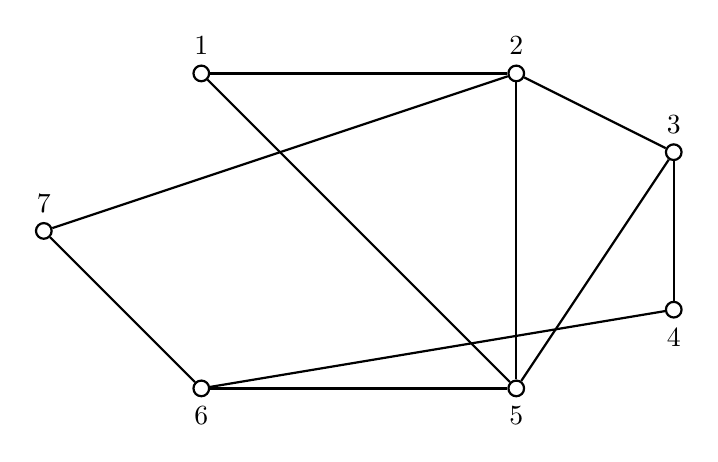
\begin{tikzpicture}
[nodedecorate/.style={shape=circle,inner sep=2pt,draw,thick},%
  linedecorate/.style={-,thick}]
%% nodes or vertices
\foreach \nodename/\x/\y/\direction/\navigate in {2/4/4/above/north,
  1/0/4/above/north, 3/6/3/above/north, 4/6/1/below/south,
  5/4/0/below/south, 7/-2/2/above/north, 6/0/0/below/south} {
  \node (\nodename) at (\x,\y) [nodedecorate] {};
  \node [\direction] at (\nodename.\navigate) {$\nodename$};
}
%% edges or lines
\path
\foreach \startnode/\endnode in {1/2, 1/5, 2/3, 2/5, 2/7, 3/4, 3/5,
  4/6, 5/6, 6/7} {
  (\startnode) edge[linedecorate] node {} (\endnode)
};
\end{tikzpicture}
}
%%
\qquad
\subfigure[]{
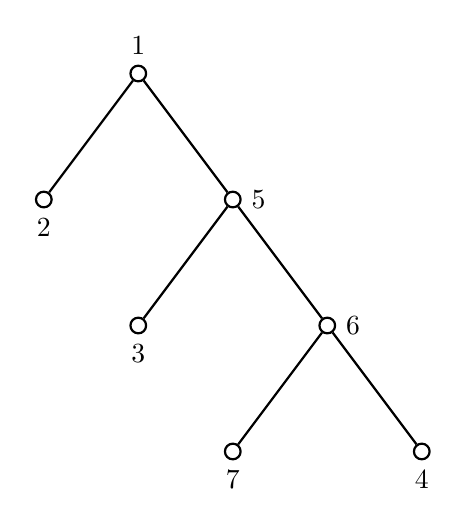
\begin{tikzpicture}
[nodedecorate/.style={shape=circle,inner sep=2pt,draw,thick},%
  linedecorate/.style={-,thick},%
  scale=1.6]
%% nodes or vertices
\foreach \nodename/\x/\y/\direction/\navigate in {
  1/1.25/3/above/north, 2/0.5/2/below/south, 5/2/2/right/east,
  3/1.25/1/below/south, 6/2.75/1/right/east, 7/2/0/below/south,
  4/3.5/0/below/south} {
  \node (\nodename) at (\x,\y) [nodedecorate] {};
  \node [\direction] at (\nodename.\navigate) {$\nodename$};
}
%% edges or lines
\path
\foreach \startnode/\endnode in {1/2, 1/5, 3/5, 5/6, 6/7, 6/4} {
  (\startnode) edge[linedecorate] node {} (\endnode)
};
\end{tikzpicture}
}
%%
%%
\subfigure[]{
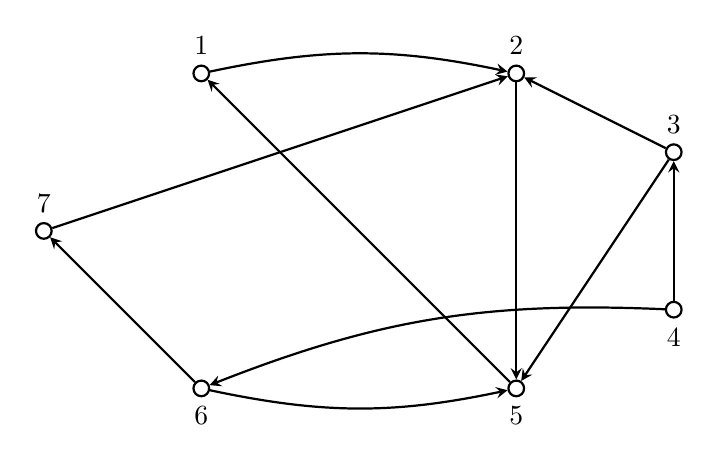
\begin{tikzpicture}
[nodedecorate/.style={shape=circle,inner sep=2pt,draw,thick},%
  arrowdecorate/.style={->,>=stealth,thick}]
%% nodes or vertices
\foreach \nodename/\x/\y/\direction/\navigate in {2/4/4/above/north,
  1/0/4/above/north, 3/6/3/above/north, 4/6/1/below/south,
  5/4/0/below/south, 7/-2/2/above/north, 6/0/0/below/south} {
  \node (\nodename) at (\x,\y) [nodedecorate] {};
  \node [\direction] at (\nodename.\navigate) {$\nodename$};
}
%% edges or lines
\path
\foreach \startnode/\endnode in {2/5, 3/2, 3/5, 4/3, 5/1, 6/7, 7/2} {
  (\startnode) edge[arrowdecorate] node {} (\endnode)
}
\foreach \startnode/\endnode/\benddirection/\angle in {
  1/2/bend left/12, 4/6/bend right/12, 6/5/bend right/12} {
  (\startnode) edge[arrowdecorate,\benddirection=\angle] node {} (\endnode)
};
\end{tikzpicture}
}
%%
\qquad
\subfigure[]{
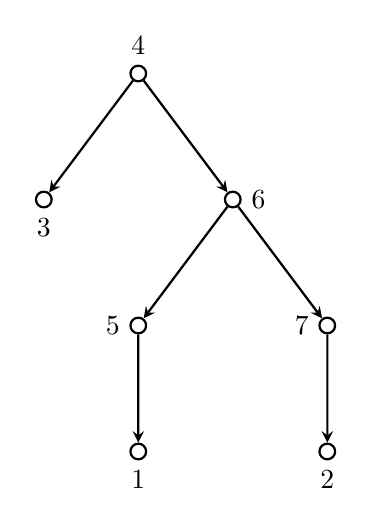
\begin{tikzpicture}
[nodedecorate/.style={shape=circle,inner sep=2pt,draw,thick},%
  arrowdecorate/.style={->,>=stealth,thick},
  scale=1.6]
%% nodes or vertices
\foreach \nodename/\x/\y/\direction/\navigate in {
  4/1.25/3/above/north, 3/0.5/2/below/south, 6/2/2/right/east,
  5/1.25/1/left/west, 7/2.75/1/left/west, 1/1.25/0/below/south,
  2/2.75/0/below/south} {
  \node (\nodename) at (\x,\y) [nodedecorate] {};
  \node [\direction] at (\nodename.\navigate) {$\nodename$};
}
%% edges or lines
\path
\foreach \startnode/\endnode in {4/3, 4/6, 6/5, 6/7, 5/1, 7/2} {
  (\startnode) edge[arrowdecorate] node {} (\endnode)
};
\end{tikzpicture}
}
\caption{Depth-first search trees for undirected and directed graphs.}
\label{fig:graph_algorithms:depth_first_search_undirected}
\end{figure}


%%%%%%%%%%%%%%%%%%%%%%%%%%%%%%%%%%%%%%%%%%%%%%%%%%%%%%%%%%%%%%%%%%%%%%%%%%%

\subsection{Connectivity of a graph}

Both BFS and DFS can be used to determine if an undirected graph is
connected. Let $G = (V, E)$ be an undirected graph of order $n > 0$
and let $s$ be an arbitrary vertex of $G$. We initialize a counter
$c \leftarrow 1$ to mean that we are starting our exploration at $s$,
hence we have already visited one vertex, i.e. $s$. We apply either
BFS or DFS, treating $G$ and $s$ as input to any of these
algorithms. Each time we visit a vertex that was previously unvisited,
we increment the counter $c$. At the end of the algorithm, we compare
$c$ with $n$. If $c = n$, we know that we have visited all vertices of
$G$ and conclude that $G$ is connected. Otherwise, we conclude that
$G$ is disconnected. This procedure is summarized in
Algorithm~\ref{alg:graph_algorithms:graph_connectivity}.

\begin{algorithm}[!htpb]
\dontprintsemicolon  % no semicolon at end of pseudocode statements
%% data section
\SetKwInOut{Input}{Input}
\SetKwInOut{Output}{Output}
\SetKwData{False}{False}
\SetKwData{True}{True}
%% input/output
\Input{An undirected graph $G = (V, E)$ of order $n > 0$. A vertex $s$
  from which to start the search. The vertices are numbered from $1$
  to  $n = |V|$, i.e. $V = \{1, 2, \dots, n\}$.}
\Output{$\True$ if $G$ is connected; $\False$ otherwise.}
\BlankLine
$Q \leftarrow [s]$~\tcc*[f]{queue of nodes to visit}\;
$D \leftarrow [0, 0, \dots, 0]$~\tcc*[f]{$n$ copies of $0$}\;
$D[s] \leftarrow 1$\;
$c \leftarrow 1$\;
\While{$\length(Q) > 0$}{
  $v \leftarrow \dequeue(Q)$\;
  \For{\emph{each} $w \in \adj(v)$}{
    \If{$D[w] = 0$}{
      $D[w] \leftarrow 1$\;
      $c \leftarrow c + 1$\;
      $\enqueue(Q, w)$\;
    }
  }
}
\If{$c = |V|$~\nllabel{alg:BFS:connectivity_test}}{
  \Return \True\;
} \Else{
  \Return \False\;
}
\caption{Determining whether an undirected graph is connected.}
\label{alg:graph_algorithms:graph_connectivity}
\end{algorithm}

Note that Algorithm~\ref{alg:graph_algorithms:graph_connectivity} uses
the BFS template of
Algorithm~\ref{alg:graph_algorithms:breadth_first_search_template},
with some minor changes. Instead of initializing the list $D$ with
$n = |V|$ copies of $\infty$, we use $n$ copies of $0$. Each time we
have visited a vertex $w$, we make the assignment $D[w] \leftarrow 1$,
instead of incrementing the value $D[v]$ of $w$'s parent vertex and
assign that value to $D[w]$. At the end of the while loop, we have the
equality $c = \sum_{d \in D} d$. The value of this sum could be used
in the test starting from line~\ref{alg:BFS:connectivity_test}.
However, the value of the counter $c$ is incremented immediately after
we have visited an unvisited vertex. An advantage is that we do not
need to perform a separate summation outside of the while loop. To use
the DFS template for determining graph connectivity, we simply replace
the queue implementation in
Algorithm~\ref{alg:graph_algorithms:graph_connectivity} with a stack
implementation.


%%%%%%%%%%%%%%%%%%%%%%%%%%%%%%%%%%%%%%%%%%%%%%%%%%%%%%%%%%%%%%%%%%%%%%%%%%%

\section{Weights and distances}

In Chapter~\ref{chap:introduction}, we briefly mentioned some
applications of weighted graphs, but we did not define the concept of
weighted graphs. A graph is said to be
\emph{weighted}\index{weighted graph} when we assign a numeric label
or weight to each of its edges. Depending on the application, we can
let the vertices represent physical locations and interpret the weight
of an edge as the distance separating two adjacent vertices. There
might be a cost involved in travelling from a vertex to one of its
neighbors, in which case the weight assigned to the corresponding edge
can represent such a cost. The concept of
\emph{weighted digraphs}\index{weighted digraph} can be similarly
defined. When no explicit weights are assigned to the edges of an
undirected graph or digraph, it is usually convenient to consider each
edge as having a weight of one.

Based on the concept of weighted graphs, we now define what it means
for a path to be a shortest path. Let $G = (V,E)$ be a (di)graph with
non-negative edge weights $w(e)$ for each edge $e \in E$. The
\emph{length}\index{path!length} or
\emph{distance}\index{path!distance} $d(P)$ of a path $P$ from
$v \in V$ to $w \in V$ is the sum of the edge weights for edges in
$P$. Denote by $d(v,w)$ the smallest value of $d(P)$ for all paths $P$
from $v$ to $w$. When we regard edge weights as physical distances, a
$v$-$w$ path that realizes $d(v,w)$ is sometimes called a
\emph{shortest path}\index{path!shortest} from $v$ to $w$.

The distance function $d$ on a graph with nonnegative edge weights is
known as a \emph{metric function}. Intuitively, the distance between
two physical locations is greater than zero. When these two locations
coincide, i.e. they are one and the same location, the distance
separating them is zero. Regardless of whether we are measuring the
distance from location $a$ to $b$ or from $b$ to $a$, we would obtain
the same distance. Imagine now a third location $c$. The distance from
$a$ to $b$ plus the distance from $b$ to $c$ is greater than or equal
to the distance from $a$ to $c$. The latter principle is known as the
\emph{triangle inequality}. In summary, given three vertices $u,v,w$
in a connected graph $G$, the distance function $d$ on $G$ satisfies
the following property.

\begin{lemma}
Let $G = (V,E)$ be a connected graph with a positive weight function
$w: E \longrightarrow \RR^{+}$. Define a distance function
$d: V \times V \longrightarrow \RR$ given by
\[
d(u,v)
=
\begin{cases}
\infty, & \text{if there are no paths from $u$ to $v$}, \\
\min\{w(W) \;|\; \text{$W$ is a $u$-$v$ walk}\}, & \text{otherwise}.
\end{cases}
\]
Then $d$ satisfies the following properties:
%
\begin{enumerate}
\item Nonnegativity: $d(u,v) \geq 0$ with $d(u,v) = 0$ if and only if
  $u = v$.

\item Symmetry: $d(u,v) = d(v,u)$.

\item Triangle inequality: $d(u,v) + d(v,w) \geq d(u,w)$.
\end{enumerate}
\end{lemma}

The pair $(V, d)$ is called a \emph{metric space}, where the word
``metric'' refers to the distance function $d$. Any graphs we consider
are assumed to have finite sets of vertices. For this reason, $(V,d)$
is also known as a \emph{finite metric space}. The distance matrix
$D = [d(v_i, v_j)]$ of a connected graph is the distance matrix of its
finite metric space. The topic of metric space is covered in further
details in topology texts such as Runde~\cite{Runde2005} and Shirali
and Vasudeva~\cite{ShiraliVasudeva2006}.

Many different algorithms exist for computing a shortest path in a
weighted graph. Some only work if the graph has no negative weight
cycles. Some assume that there is a single start or source
vertex. Some compute the shortest paths from any vertex to any other,
and also detect if the graph has a negative weight cycle. No matter
what algorithm is used for the special case of non-negative weights,
the length of the shortest path can neither equal nor exceed the order
of the graph.

\begin{lemma}
\label{lem:graph_algorithms:shortest_path_length}
Fix a vertex $v$ in a connected graph $G = (V,E)$ of order
$n = |V|$. If there are no negative weight cycles in $G$, then there
exists a shortest path from $v$ to any other vertex $w \in V$ that
uses at most $n - 1$ edges.
\end{lemma}

\begin{proof}
Suppose that $G$ contains no negative weight cycles. Observe that at
most $n - 1$ edges are required to construct a path from $v$ to any
vertex $w$
(Corollary~\ref{cor:introduction:any_path_has_length_at_most_n_minus_1}).
Let $P$ denote such a path:
\[
P: v_0 = v,\, v_1,\, v_2, \dots, v_k = w.
\]
Since $G$ has no negative weight cycles, the weight of $P$ is no less
than the weight of $P'$, where $P'$ is the same as $P$ except that all
cycles have been removed. Thus, we can remove all cycles from $P$ and
obtain a $v$-$w$ path $P'$ of lower weight. Since the final path is
acyclic, it must have no more than $n - 1$ edges.
\end{proof}

\begin{algorithm}[!htpb]
\dontprintsemicolon  % no semicolon at end of pseudocode statements
%% data section
\SetKwInOut{Input}{Input}
\SetKwInOut{Output}{Output}
%% input/output
\Input{A weighted graph or digraph $G = (V, E)$, where the vertices
  are numbered as $V = \{1, 2, \dots, n\}$. A starting vertex $s$.}
\Output{A list $D$ of distances from $s$ to all other vertices. A list
  $P$ of parent vertices such that $P[v]$ is the parent of $v$.}
\BlankLine
$D \leftarrow [\infty, \infty, \dots, \infty]$~\tcc*[f]{$n$ copies of $\infty$}\;
let $C$ be a list of candidate vertices to visit\;
\While{$\length(C) > 0$}{
  select $v \in C$\;
  $C \leftarrow \remove(C, v)$\;
  \For{\emph{each} $u \in \adj(v)$~\nllabel{alg:generic_shortest_path:neighbors}}{
    \If{$D[u] > D[v] + w(vu)$}{
      $D[u] \leftarrow D[v] + w(vu)$\;
      $P[u] \leftarrow v$\;
      if $u$ is not in $C$, add $u$ to $C$\;
    }
  }
}
\Return $(D,P)$\;
\caption{A template for shortest path algorithms.}
\label{alg:graph_algorithms:generic_shortest_path_algorithm}
\end{algorithm}

Having defined weights and distances, we are now ready to discuss
shortest path algorithms for weighted graphs. The breadth-first search
Algorithm~\ref{alg:graph_algorithms:breadth_first_search_template} can
be applied where each edge has unit weight. Moving on to the general
case of graphs with positive edge weights, algorithms for determining
shortest paths in such graphs can be classified as
\emph{weight-setting} or
\emph{weight-corrrecting}~\cite{GalloPallottino1986}. A weight-setting
method traverses a graph and assigns weights that, once assigned,
remain unchanged for the duration of the algorithm. Weight-setting
algorithms cannot deal with negative weights. On the other hand, a
weight-correcting method is able to change the value of a weight many
times while traversing a graph. In contrast to a weight-setting
algorithm, a weight-correcting algorithm is able to deal with negative
weights, provided that the weight sum of any cycle is
nonnegative. The term \emph{negative cycle} refers to the weight sum $s$
of a cycle such that $s < 0$.

Algorithm~\ref{alg:graph_algorithms:generic_shortest_path_algorithm}
is a general template for many shortest path algorithms. With a tweak
here and there, one could modify it to suit the problem at hand. Note
that $w(vu)$ is the weight of the edge $vu$. If the input graph is
undirected, line~\ref{alg:generic_shortest_path:neighbors} considers
all the neighbors of $v$. For digraphs, we are interested in
out-neighbors of $v$ and accordingly we replace ``$u \in \adj(v)$'' in
line~\ref{alg:generic_shortest_path:neighbors} with
``$u \in \oadj(v)$''. The general flow of
Algorithm~\ref{alg:graph_algorithms:generic_shortest_path_algorithm}
follows the same pattern as depth-first and breadth-first searches.


%%%%%%%%%%%%%%%%%%%%%%%%%%%%%%%%%%%%%%%%%%%%%%%%%%%%%%%%%%%%%%%%%%%%%%%%%%%

\section{Dijkstra's algorithm}
\label{sec:graph_algorithms:Dijkstra_algorithm}

Dijkstra's algorithm~\cite{Dijkstra1959}, discovered by E. W.~Dijkstra
in 1959, is a graph search algorithm that solves the single-source
shortest path problem for a graph with nonnegative edge
weights. Imagine that the vertices of a weighted graph represent
cities and edge weights represent distances between pairs of cities
connected by a direct road. Dijkstra's algorithm can be used to find a
shortest route from a fixed city to any other city.

Let $G = (V,E)$ be a (di)graph with nonnegative edge weights. Fix a
start or source vertex $s \in V$. Dijkstra's
Algorithm~\ref{alg:graph_algorithms:dijkstra_general} performs a
number of steps, basically one step for each vertex in $V$. First, we
initialize a list $D$ with $n$ copies of $\infty$ and then assign $0$
to $D[s]$. The purpose of the symbol $\infty$ is to denote the largest
possible value. The list $D$ is to store the distances of all shortest
paths from $s$ to any other vertices in $G$, where we take the
distance of $s$ to itself to be zero. The list $P$ of parent vertices
is initially empty and the queue $Q$ is initialized to all vertices in
$G$. We now consider each vertex in $Q$, removing any vertex after we
have visited it. The while loop starting on
line~\ref{alg:dijkstra_general:while_loop} runs until we have visited
all
vertices. Line~\ref{alg:dijkstra_general:find_vertex_minimal_distance}
chooses which vertex to visit, preferring a vertex $v$ whose distance
value $D[v]$ from $s$ is minimal. After we have determined such a
vertex $v$, we remove it from the queue $Q$ to signify that we have
visited $v$. The for loop starting on
line~\ref{alg:dijkstra_general:for_loop} adjusts the distance values
of each neighbor $u$ of $v$ such that $u$ is also in $Q$. If $G$ is
directed, we only consider out-neighbors of $v$ that are also in
$Q$. The conditional starting on
line~\ref{alg:dijkstra_general:if_relaxation} is where the adjustment
takes place. The expression $D[v] + w(vu)$ sums the distance from $s$
to $v$ and the distance from $v$ to $u$. If this total sum is less
than the distance $D[u]$ from $s$ to $u$, we assign this lesser
distance to $D[u]$ and let $v$ be the parent vertex of $u$. In this
way, we are choosing a neighbor vertex that results in minimal
distance from $s$. Each pass through the while loop decreases the
number of elements in $Q$ by one without adding any elements to
$Q$. Eventually, we would exit the while loop and the algorithm
returns the lists $D$ and $P$.

\begin{algorithm}[!htpb]
\dontprintsemicolon  % no semicolon at end of pseudocode statements
%% data section
\SetKwInOut{Input}{Input}
\SetKwInOut{Output}{Output}
%% input/output
\Input{An undirected or directed graph $G = (V, E)$ that is weighted
  and has no self-loops. The order of $G$ is $n > 0$. A vertex $s \in V$
  from which to start the search. Vertices are numbered from 1 to $n$,
  i.e. $V = \{1, 2, \dots, n\}$.}
\Output{A list $D$ of distances such that $D[v]$ is the distance of a
  shortest path from $s$ to $v$. A list $P$ of vertex parents such
  that $P[v]$ is the parent of $v$, i.e. $v$ is adjacent from $P[v]$.}
\BlankLine
%% algorithm body
$D \leftarrow [\infty, \infty, \dots, \infty]$~\tcc*[f]{$n$ copies of $\infty$}\;
$D[s] \leftarrow 0$\;
$P \leftarrow [\,]$\;
$Q \leftarrow V$~\tcc*[f]{list of nodes to visit}\;
\While{$\length(Q) > 0$~\nllabel{alg:dijkstra_general:while_loop}}{
  find $v \in Q$ such that $D[v]$ is minimal~\nllabel{alg:dijkstra_general:find_vertex_minimal_distance}\;
  $Q \leftarrow \remove(Q, v)$\;
  \For{\emph{each} $u \in \adj(v) \cap Q$~\nllabel{alg:dijkstra_general:for_loop}}{
    \If{$D[u] > D[v] + w(vu)$~\nllabel{alg:dijkstra_general:if_relaxation}}{
      $D[u] \leftarrow D[v] + w(vu)$\;
      $P[u] \leftarrow v$\;
    }
  }
}
\Return $(D, P)$\;
\caption{A general template for Dijkstra's algorithm.}
\label{alg:graph_algorithms:dijkstra_general}
\end{algorithm}

\begin{figure}[!htbp]
\centering
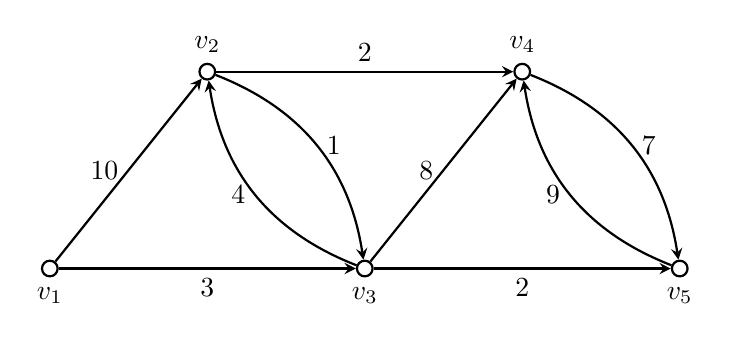
\begin{tikzpicture}
[nodedecorate/.style={shape=circle,inner sep=2pt,draw,thick},%
  arrowdecorate/.style={->,>=stealth,thick}]
%% nodes or vertices
\foreach \nodename/\x/\y/\direction/\navigate in {
  v_1/0/0/below/south, v_2/2/2.5/above/north, v_3/4/0/below/south,
  v_4/6/2.5/above/north, v_5/8/0/below/south} {
  \node (\nodename) at (\x,\y) [nodedecorate] {};
  \node [\direction] at (\nodename.\navigate) {$\nodename$};
}
%% edges or lines
\path
\foreach \startnode/\endnode/\direction/\weight in {
  v_1/v_2/left/10, v_1/v_3/below/3, v_2/v_4/above/2, v_3/v_4/left/8,
  v_3/v_5/below/2} {
  (\startnode) edge[arrowdecorate] node[\direction]{$\weight$} (\endnode)
}
\foreach \startnode/\endnode/\direction/\weight in {
  v_3/v_2/left/4, v_2/v_3/right/1, v_4/v_5/right/7, v_5/v_4/left/9} {
  (\startnode) edge[arrowdecorate,bend left] node[\direction]{$\weight$} (\endnode)
};
\end{tikzpicture}
\caption{Searching a weighted digraph using Dijkstra's algorithm.}
\label{fig:graph_algorithms:Dijkstra_algorithm_digraph}
\end{figure}
%% sage: M = matrix([[0,10,3,0,0],[0,0,1,2,0],[0,4,0,8,2],[0,0,0,0,7],[0,0,0,9,0]])
%% sage: D = DiGraph(M, format="weighted_adjacency_matrix")
%% sage: D.plot(edge_labels=True, graph_border=True).show()
%%
%% sage: G = DiGraph({1: {2:10, 3:3},
%% ....: 2: {3:1, 4:2},
%% ....: 3: {2:4, 4:8, 5:2},
%% ....: 4: {5:7},
%% ....: 5: {4:9}}, implementation=''c_graph'')
%% sage: G.shortest_paths(1, by_weight=True)
%% {1: [1], 2: [1, 3, 2], 3: [1, 3], 4: [1, 3, 2, 4], 5: [1, 3, 5]}

\begin{table}[!htbp]
\centering
\begin{tabular}{ccccc} \hline
$v_1$               & $v_2$                 & $v_3$                 & $v_4$                 & $v_5$ \\\hline
\underline{$(0,-)$} & $(\infty,-)$          & $(\infty,-)$          & $(\infty,-)$          & $(\infty,-)$ \\
                    & $(10,v_1)$            & \underline{$(3,v_1)$} & $(11,v_3)$            & \underline{$(5,v_3)$} \\
                    & \underline{$(7,v_3)$} &                       & \underline{$(9,v_2)$} & \\\hline
\end{tabular}
\caption{Stepping through Dijkstra's algorithm.}
\label{tab:graph_algorithms:working_through_Dijkstra_algorithm}
\end{table}

\begin{example}
Apply Dijkstra's algorithm to the graph in
Figure~\ref{fig:graph_algorithms:Dijkstra_algorithm_digraph}, with
starting vertex $v_1$.
\end{example}

\begin{proof}[Solution]
Dijkstra's Algorithm~\ref{alg:graph_algorithms:dijkstra_general}
applied to the graph in
Figure~\ref{fig:graph_algorithms:Dijkstra_algorithm_digraph} yields
Table~\ref{tab:graph_algorithms:working_through_Dijkstra_algorithm}. For
any column $v_i$ in the table, each 2-tuple represents the distance
and parent vertex of $v_i$. As we move along the graph, processing
vertices according to Dijkstra's algorithm, the distance and parent
vertex of a column are updated. The underlined 2-tuple represents the
final distance and parent vertex produced by Dijkstra's
algorithm. From
Table~\ref{tab:graph_algorithms:working_through_Dijkstra_algorithm},
we have the following shortest paths and distances:
\[
\begin{array}{ll}
v_1\text{-}v_2: v_1, v_3, v_2      &\quad d(v_1, v_2) = 7 \\[4pt]
v_1\text{-}v_3: v_1, v_3           &\quad d(v_1, v_3) = 3 \\[4pt]
v_1\text{-}v_4: v_1, v_3, v_2, v_4 &\quad d(v_1, v_4) = 9 \\[4pt]
v_1\text{-}v_5: v_1, v_3, v_5      &\quad d(v_1, v_5) = 5
\end{array}
\]
Intermediary vertices for a $u$-$v$ path are obtained by starting from
$v$ and work backward using the parent of $v$, then the parent of the
parent, and so on.
\end{proof}

Dijkstra's algorithm is an example of a \emph{greedy algorithm}.
Whenever it tries to find the next vertex, it chooses only that vertex
that minimizes the total weight so far. Greedy algorithms may not
produce the best possible result. However, as the following theorem
shows, Dijkstra's algorithm does indeed produce shortest paths.

\begin{theorem}
\textbf{Correctness of
  Algorithm~\ref{alg:graph_algorithms:dijkstra_general}.}
Let $G = (V, E)$ be a weighted (di)graph with a nonnegative weight
function $w$. When Dijkstra's algorithm is applied to $G$ with source
vertex $s \in V$, the algorithm terminates with $D[u] = d(s,u)$ for
all $u \in V$. Furthermore, if $D[v] \neq \infty$ and $v \neq s$, then
$s=u_1, u_2, \dots, u_k = v$ is a shortest $s$-$v$ path such that
$u_{i-1} = P[u_i]$ for $i = 2,3,\dots,k$.
\end{theorem}

\begin{proof}
If $G$ is disconnected, then any $v \in V$ that cannot be reached from
$s$ has distance $D[v] = \infty$ upon algorithm termination. Hence, it
suffices to consider the case where $G$ is connected. Let
$V = \{s=v_1, v_2, \dots, v_n\}$ and use induction on $i$ to show that
after visiting $v_i$ we have
%
\begin{equation}
\label{eq:graph_algorithms:Dijkstra:shortest_distance}
D[v]
=
d(s,v)
\qquad
\text{for all $v \in V_i = \{v_1, v_2, \dots, v_i\}$}.
\end{equation}
%
For $i = 1$, equality holds. Assume for induction
that~(\ref{eq:graph_algorithms:Dijkstra:shortest_distance}) holds for
some $1 \leq i \leq n - 1$, so that now our task is to show
that~(\ref{eq:graph_algorithms:Dijkstra:shortest_distance}) holds for
$i + 1$. To verify $D[v_{i+1}] = d(s, v_{i+1})$, note that by our
inductive hypothesis,
\[
D[v_{i+1}]
=
\min \left\{
\left. d(s,v) + w(vu) \;\right|\;
v \in V_i \text{ and } u \in \adj(v) \cap (Q \backslash V_i)
\right\}
\]
and respectively
\[
D[v_{i+1}]
=
\min \left\{
\left. d(s,v) + w(vu) \;\right|\;
v \in V_i \text{ and } u \in \oadj(v) \cap (Q \backslash V_i)
\right\}
\]
if $G$ is directed. Therefore, $D[v_{i+1}] = d(s, v_{i+1})$.

Let $v \in V$ such that $D[v] \neq \infty$ and $v \neq s$. We now
construct an $s$-$v$ path. When
Algorithm~\ref{alg:graph_algorithms:dijkstra_general} terminates, we
have $D[v] = D[v_1] + w(v_1 v)$, where $P[v] = v_1$ and
$d(s,v) = d(s, v_1) + w(v_1 v)$. This means that $v_1$ is the
second-to-last vertex in a shortest $s$-$v$ path. Repeated application
of this process using the parent list $P$, we eventually produce a
shortest $s$-$v$ path $s=v_m, v_{m-1}, \dots, v_1, v$, where
$P[v_i] = v_{i+1}$ for $i = 1, 2, \dots, m - 1$.
\end{proof}

To analyze the worst case time complexity of
Algorithm~\ref{alg:graph_algorithms:dijkstra_general}, note that
initializing $D$ takes $O(n + 1)$ and initializing $Q$ takes $O(n)$,
for a total of $O(n)$ devoted to initialization. Each extraction of a
vertex $v$ with minimal $D[v]$ requires $O(n)$ since we search through
the entire list $Q$ to determine the minimum value, for a total of
$O(n^2)$. Each insertion into $D$ requires constant time and the same
holds for insertion into $P$. Thus, insertion into $D$ and $P$ takes
$O(|E| + |E|) = O(|E|)$, which require at most $O(n)$ time. In the
worst case, Dijkstra's
Algorithm~\ref{alg:graph_algorithms:dijkstra_general} has running time
$O(n^2 + n) = O(n^2)$.

Can we improve the run time of Dijkstra's algorithm? The time
complexity of Dijkstra's algorithm depends on its implementation. With
a simple list implementation as presented in
Algorithm~\ref{alg:graph_algorithms:dijkstra_general}, we have a worst
case time complexity of $O(n^2)$, where $n$ is the order of the graph
under consideration. Let $m$ be the size of the
graph. Table~\ref{tab:graph_algorithms:worst_case_time_complexity_Dijkstra}
presents time complexities of Dijkstra's algorithm for various
implementations. Out of all the four implementations in this table,
the heap implementations are much more efficient than the list
implementation presented in
Algorithm~\ref{alg:graph_algorithms:dijkstra_general}. A heap is a type
of tree, a topic which will be covered in
Chapter~\ref{chap:trees_forests}.

\begin{table}[!htbp]
\centering
\begin{tabular}{ll} \hline
Implementation & Time complexity \\\hline
list           & $O(n^2)$ \\
binary heap    & $O \big( \log(n) \cdot (n + m) \big)$ \\
$k$-ary heap   & $O \big( (kn + m) \frac{\log(n)}{\log(k)} \big)$ \\
Fibonacci heap & $O(n \cdot \log(n) + m)$ \\\hline
\end{tabular}
\caption{Implementation specific worst case time complexity of
  Dijkstra's algorithm.}
\label{tab:graph_algorithms:worst_case_time_complexity_Dijkstra}
\end{table}


%%%%%%%%%%%%%%%%%%%%%%%%%%%%%%%%%%%%%%%%%%%%%%%%%%%%%%%%%%%%%%%%%%%%%%%%%%%

\section{Bellman-Ford algorithm}

\begin{quote}
\includegraphics[scale=2.5]{image/pillow-talk-bellman-ford} \\
\noindent
--- Randall Munroe\index{Munroe, Randall}, xkcd,
\url{http://xkcd.com/69/}
\end{quote}

\noindent
A disadvantage of Dijkstra's
Algorithm~\ref{alg:graph_algorithms:dijkstra_general} is that it
cannot handle graphs with negative edge weights. The Bellman-Ford
algorithm computes single-source shortest paths in a weighted graph or
digraph, where some of the edge weights may be negative. This
algorithm is a modification of the one published in 1957 by Richard E.
Bellman~\cite{Bellman1957} and that by Lester Randolph Ford,
Jr.~\cite{Ford1956} in 1956. Shimbel~\cite{Shimbel1955} independently
discovered the same method in~1955, and Moore~\cite{Moore1959}
in~1959. In contrast to the ``greedy'' approach that Dijkstra's
algorithm takes, i.e. searching for the ``cheapest'' path, the
Bellman-Ford algorithm searches over all edges and keeps track of the
shortest one found as it searches.

\begin{algorithm}[!htpb]
\dontprintsemicolon  % no semicolon at end of pseudocode statements
%% data section
\SetKwInOut{Input}{Input}
\SetKwInOut{Output}{Output}
\SetKwData{False}{False}
%% input/output
\Input{An undirected or directed graph $G = (V, E)$ that is weighted
  and has no self-loops. Negative edge weights are allowed. The order
  of $G$ is $n > 0$. A vertex $s \in V$ from which to start the
  search. Vertices are numbered from 1 to $n$, i.e.
  $V = \{1, 2, \dots, n\}$.}
\Output{A list $D$ of distances such that $D[v]$ is the distance of a
  shortest path from $s$ to $v$. A list $P$ of vertex parents such
  that $P[v]$ is the parent of $v$, i.e. $v$ is adjacent from
  $P[v]$. If $G$ has negative-weight cycles, then return
  \False. Otherwise, return $D$ and $P$.}
\BlankLine
%% algorithm body
$D \leftarrow [\infty, \infty, \dots, \infty]$~\tcc*[f]{$n$ copies of $\infty$}~\nllabel{alg:Bellman_Ford:init_infinity}\;
$D[s] \leftarrow 0$\;
$P \leftarrow [\,]$~\nllabel{alg:Bellman_Ford:init_parent_list}\;
\For{$i \leftarrow 1, 2, \dots, n-1$~\nllabel{alg:Bellman_Ford:for_loop:relax}}{
  \For{\emph{each edge} $uv \in E$}{
    \If{$D[v] > D[u] + w(uv)$}{
      $D[v] \leftarrow D[u] + w(uv)$\;
      $P[v] \leftarrow u$\;
    }
  }
  \nllabel{alg:Bellman_Ford:for_loop:end_relax}
}
\For{\emph{each edge} $uv \in E$~\nllabel{alg:Bellman_Ford:for_loop:check_negative_weight_cycles}}{
  \If{$D[v] > D[u] + w(uv)$}{
    \Return \False\;
  }
}
\Return $(D, P)$\;
\caption{The Bellman-Ford algorithm.}
\label{alg:graph_algorithms:Bellman_Ford}
\end{algorithm}

The Bellman-Ford Algorithm~\ref{alg:graph_algorithms:Bellman_Ford}
runs in time $O(mn)$, where $m$ and $n$ are the size and order of an
input graph, respectively. To see this, note that the initialization
on lines~\ref{alg:Bellman_Ford:init_infinity}
to~\ref{alg:Bellman_Ford:init_parent_list} takes $O(n)$. Each of the
$n - 1$ rounds of the for loop starting on
line~\ref{alg:Bellman_Ford:for_loop:relax} takes $O(m)$, for a total
of $O(mn)$ time. Finally, the for loop starting on
line~\ref{alg:Bellman_Ford:for_loop:check_negative_weight_cycles}
takes $O(m)$.

The loop starting on line~\ref{alg:Bellman_Ford:for_loop:relax}
performs at most $n - 1$ updates of the distance $D[v]$ of each head
of an edge. Many graphs have sizes that are less then $n - 1$,
resulting in a number of redundant rounds of updates. To avoid such
redundancy, we could add an extra check in the outer loop spanning
lines~\ref{alg:Bellman_Ford:for_loop:relax}
to~\ref{alg:Bellman_Ford:for_loop:end_relax} to immediately terminate
that outer loop after any round that did not result in an update of
any $D[v]$.
Algorithm~\ref{alg:graph_algorithms:Bellman_Ford:redundant_updates}
presents a modification of the Bellman-Ford
Algorithm~\ref{alg:graph_algorithms:Bellman_Ford} that avoids
redundant rounds of updates.

\begin{algorithm}[!htpb]
\dontprintsemicolon  % no semicolon at end of pseudocode statements
%% data section
\SetKwInOut{Input}{Input}
\SetKwInOut{Output}{Output}
\SetKwData{False}{False}
\SetKwData{True}{True}
\SetKwData{Updated}{updated}
%% input/output
\Input{An undirected or directed graph $G = (V, E)$ that is weighted
  and has no self-loops. Negative edge weights are allowed. The order
  of $G$ is $n > 0$. A vertex $s \in V$ from which to start the
  search. Vertices are numbered from 1 to $n$, i.e.
  $V = \{1, 2, \dots, n\}$.}
\Output{A list $D$ of distances such that $D[v]$ is the distance of a
  shortest path from $s$ to $v$. A list $P$ of vertex parents such
  that $P[v]$ is the parent of $v$, i.e. $v$ is adjacent from
  $P[v]$. If $G$ has negative-weight cycles, then return
  \False. Otherwise, return $D$ and $P$.}
\BlankLine
%% algorithm body
$D \leftarrow [\infty, \infty, \dots, \infty]$~\tcc*[f]{$n$ copies of $\infty$}~\nllabel{alg:Bellman_Ford:init_infinity}\;
$D[s] \leftarrow 0$\;
$P \leftarrow [\,]$\;
\For{$i \leftarrow 1, 2, \dots, n-1$}{
  $\Updated \leftarrow \False$\;
  \For{\emph{each edge} $uv \in E$}{
    \If{$D[v] > D[u] + w(uv)$}{
      $D[v] \leftarrow D[u] + w(uv)$\;
      $P[v] \leftarrow u$\;
      $\Updated \leftarrow \True$\;
    }
  }
  \If{$\Updated = \False$}{
    exit the loop\;
  }
}
\For{\emph{each edge} $uv \in E$}{
  \If{$D[v] > D[u] + w(uv)$}{
    \Return \False\;
  }
}
\Return $(D, P)$\;
\caption{The Bellman-Ford algorithm with checks for redundant updates.}
\label{alg:graph_algorithms:Bellman_Ford:redundant_updates}
\end{algorithm}

%% The implementation below takes in a graph or digraph, and creates two
%% Python dictionaries \verb!dist! and \verb!predecessor!, keyed on the
%% list of vertices, which store the distance and shortest
%% paths. However, if a negative weight cycle exists~(in the case of a
%% digraph), then an error is raised.

%% \begin{center}
%% \fontsize{9pt}{9pt}
%% \selectfont
%% \tt
%% \begin{lstlisting}
%% def bellman_ford(Gamma, s):
%%     """
%%     Computes the shortest distance from s to all other vertices in Gamma.
%%     If Gamma has a negative weight cycle, then return an error.

%%     INPUT:

%%     - Gamma -- a graph.
%%     - s -- the source vertex.

%%     OUTPUT:

%%     - (d,p) -- pair of dictionaries keyed on the list of vertices,
%%       which store the distance and shortest paths.

%%     REFERENCE:

%%     http://en.wikipedia.org/wiki/Bellman-Ford_algorithm
%%     """
%%     P = []
%%     dist = {}
%%     predecessor = {}
%%     V = Gamma.vertices()
%%     E = Gamma.edges()
%%     for v in V:
%%         if v == s:
%%             dist[v] = 0
%%         else:
%%             dist[v] = infinity
%%         predecessor[v] = 0
%%     for i in range(1, len(V)):
%%         for e in E:
%%             u = e[0]
%%             v = e[1]
%%             wt = e[2]
%%             if dist[u] + wt < dist[v]:
%%                 dist[v] = dist[u] + wt
%%                 predecessor[v] = u
%%     # check for negative-weight cycles
%%     for e in E:
%%         u = e[0]
%%         v = e[1]
%%         wt = e[2]
%%         if dist[u] + wt < dist[v]:
%%             raise ValueError("Graph contains a negative-weight cycle")
%%     return dist, predecessor
%% \end{lstlisting}
%% \end{center}

%% Here are some examples.

%% \begin{center}
%% \fontsize{9pt}{9pt}
%% \selectfont
%% \tt
%% \begin{lstlisting}
%% sage: M = matrix([[0,1,4,0], [0,0,1,5], [0,0,0,3], [0,0,0,0]])
%% sage: G = Graph(M, format="weighted_adjacency_matrix")
%% sage: bellman_ford(G, G.vertices()[0])
%%   {0: 0, 1: 1, 2: 2, 3: 5}
%% \end{lstlisting}
%% \end{center}
%% %
%% The plot of this graph is given in
%% Figure~\ref{fig:graph_algorithms:Bellman_Ford_example}.

%% \begin{figure}[!htbp]
%% \centering
%% \begin{tikzpicture}
%% [nodedecorate/.style={shape=circle,inner sep=2pt,draw,thick},%
%%   linedecorate/.style={-,thick}]
%% % nodes or vertices
%% \node (0) at (0,0) [nodedecorate] {};
%% \node [below] at (0.south) {$0$};
%% \node (2) at (4,0) [nodedecorate] {};
%% \node [below] at (2.south) {$2$};
%% \node (1) at (1,2.5) [nodedecorate] {};
%% \node [above] at (1.north) {$1$};
%% \node (3) at (5,2.5) [nodedecorate] {};
%% \node [above] at (3.north) {$3$};
%% % edges or lines
%% \path
%% (0) edge[linedecorate] node[left]{$1$} (1)
%% (0) edge[linedecorate] node[below]{$4$} (2)
%% (1) edge[linedecorate] node[right]{$1$} (2)
%% (1) edge[linedecorate] node[above]{$5$} (3)
%% (2) edge[linedecorate] node[right]{$3$} (3);
%% \end{tikzpicture}
%% \caption{Shortest paths in a weighted graph using the Bellman-Ford
%%   algorithm.}
%% \label{fig:graph_algorithms:Bellman_Ford_example}
%% \end{figure}
%% %sage: M = matrix([[0,1,4,0],[0,0,1,5],[0,0,0,3],[0,0,0,0]])
%% %sage: G = Graph(M, format = "weighted_adjacency_matrix")
%% %sage: G.plot(graph_border=True, edge_labels=True).show()

%% The following example illustrates the case of a negative-weight cycle.

%% \begin{center}
%% \fontsize{9pt}{9pt}
%% \selectfont
%% \tt
%% \begin{lstlisting}
%% sage: M = matrix([[0,1,0,0],[1,0,-4,1],[1,1,0,0],[0,0,1,0]])
%% sage: G = DiGraph(M, format = "weighted_adjacency_matrix")
%% sage: bellman_ford(G, G.vertices()[0])
%% ---------------------------------------------------------------------------
%% ...
%% ValueError: Graph contains a negative-weight cycle
%% \end{lstlisting}
%% \end{center}
%% %
%% The plot of this graph is given in
%% Figure~\ref{fig:graph_algorithms:Bellman_Ford_negative_weights}.

%% \begin{figure}[!htbp]
%% \centering
%% \begin{tikzpicture}
%% [nodedecorate/.style={shape=circle,inner sep=2pt,draw,thick},%
%%   arrowdecorate/.style={->,>=stealth,thick}]
%% % nodes or vertices
%% \node (0) at (5,0) [nodedecorate] {};
%% \node [below] at (0.south) {$0$};
%% \node (1) at (1,0) [nodedecorate] {};
%% \node [below] at (1.south) {$1$};
%% \node (2) at (4,3) [nodedecorate] {};
%% \node [above] at (2.north) {$2$};
%% \node (3) at (0,3) [nodedecorate] {};
%% \node [above] at (3.north) {$3$};
%% % edges or lines
%% \path
%% (0) edge[arrowdecorate,bend left=15] node[below]{$1$} (1)
%% (1) edge[arrowdecorate,bend left=10] node[above]{$1$} (0)
%% (1) edge[arrowdecorate,bend left=15] node[left]{$-4$} (2)
%% (1) edge[arrowdecorate] node[left]{$1$} (3)
%% (2) edge[arrowdecorate] node[right]{$1$} (0)
%% (2) edge[arrowdecorate,bend left=15] node[right]{$1$} (1)
%% (3) edge[arrowdecorate] node[above]{$1$} (2);
%% \end{tikzpicture}
%% \caption{Searching a digraph with negative weight using the
%%   Bellman-Ford algorithm.}
%% \label{fig:graph_algorithms:Bellman_Ford_negative_weights}
%% \end{figure}
%% %sage: M = matrix([[0,1,0,0],[1,0,-4,1],[1,1,0,0],[0,0,1,0]])
%% %sage: G = Graph(M, format = "weighted_adjacency_matrix")
%% %sage: G.plot(graph_border=True, edge_labels=True).show()


%%%%%%%%%%%%%%%%%%%%%%%%%%%%%%%%%%%%%%%%%%%%%%%%%%%%%%%%%%%%%%%%%%%%%%%%%%%

\section{Floyd-Roy-Warshall algorithm}

Let $D$ be a weighted digraph of order $n$ and size $m$. Dijkstra's
Algorithm~\ref{alg:graph_algorithms:dijkstra_general} and the
Bellman-Ford Algorithm~\ref{alg:graph_algorithms:Bellman_Ford} can be
used to determine shortest paths from a single source vertex to all
other vertices of $D$. To determine a shortest path between each pair
of distinct vertices in $D$, we repeatedly apply either of these
algorithms to each vertex of $D$. Such repeated application of
Dijkstra's and the Bellman-Ford algorithms results in algorithms that
run in time $O(n^3)$ and $O(n^2m)$, respectively.

The \emph{Floyd-Roy-Warshall algorithm}~(FRW), or the Floyd-Warshall
algorithm, is an algorithm for finding shortest paths in a weighted,
directed graph. Like the Bellman-Ford algorithm, it allows for
negative edge weights and detects a negative weight cycle if one
exists. Assuming that there are no negative weight cycles, a single
execution of the FRW algorithm will find the shortest paths between
all pairs of vertices. It was discovered independently by Bernard
Roy~\cite{Roy1959} in 1959, Robert Floyd~\cite{Floyd1962} in 1962, and
by Stephen Warshall~\cite{Warshall1962} in 1962.

In some sense, the FRW algorithm is an example of
\emph{dynamic programming}, which allows one to break the computation
into simpler steps using some sort of recursive procedure. The rough
idea is as follows. Temporarily label the vertices of a weighted
digraph $G$ as $V = \{1,2,\dots,n\}$ with $n = |V(G)|$. Let
$W = [w(i,j)]$ be the weight matrix of $G$ where
%
\begin{equation}
\label{eq:graph_algorithms:Floyd_Roy_Warshall_weight_matrix}
w(i,j)
=
\begin{cases}
w(ij), & \text{if $ij \in E(G)$}, \\
0, & \text{if $i = j$}, \\
\infty, & \text{otherwise}.
\end{cases}
\end{equation}
%
Let $P_k(i,j)$ be a shortest path from $i$ to $j$ such that its
intermediate vertices are in $\{1, 2, \dots, k\}$. Let $D_k(i,j)$ be
the weight (or distance) of $P_k(i,j)$. If no shortest $i$-$j$ paths
exist, define $P_k(i,j) = \infty$ and $D_k(i,j) = \infty$ for all
$k \in \{1, 2, \dots, n\}$. If $k = 0$, then $P_0(i,j): i, j$ since no
intermediate vertices are allowed in the path and hence
$D_0(i,j) = w(i,j)$. In other words, if $i$ and $j$ are adjacent, a
shortest $i$-$j$ path is the edge $ij$ itself and the weight of this
path is simply the weight of $ij$. Now consider $P_k(i,j)$ for
$k > 0$. Either $P_k(i,j)$ passes through $k$ or it does not. If $k$
is not on the path $P_k(i,j)$, then the intermediate vertices of
$P_k(i,j)$ are in  $\{1, 2, \dots, k-1\}$, as are the vertices of
$P_{k-1}(i,j)$. In case $P_k(i,j)$ contains the vertex $k$, then
$P_k(i,j)$ traverses $k$ exactly once by the definition of path. The
$i$-$k$ subpath in $P_k(i,j)$ is a shortest $i$-$k$ path whose
intermediate vertices are drawn from $\{1, 2, \dots, k-1\}$, which is
also the set of intermediate vertices for the $k$-$j$ subpath in
$P_k(i,j)$. That is, to obtain $P_k(i,j)$, we take the union of the
paths $P_{k-1}(i,k)$ and $P_{k-1}(k,j)$. We compute the weight
$D_k(i,j)$ of $P_k(i,j)$ using the expression
%
\begin{equation}
\label{eq:graph_algorithms:Floyd_Roy_Warshall:shortest_path_weights}
D_k(i,j)
=
\begin{cases}
w(i,j), & \text{if $k = 0$}, \\
\min\{D_{k-1}(i,j),\, D_{k-1}(i,k) + D_{k-1}(k,j)\}, & \text{if $k > 0$}.
\end{cases}
\end{equation}

The key to the Floyd-Roy-Warshall algorithm lies in exploiting
expression~(\ref{eq:graph_algorithms:Floyd_Roy_Warshall:shortest_path_weights}).
If $n = |V|$, then this is a $O(n^3)$ time algorithm. For
comparison, the Bellman-Ford algorithm has complexity
$O(|V| \cdot |E|)$, which is $O(n^3)$ time for dense graphs. However,
Bellman-Ford only yields the shortest paths emanating from a
\emph{single} vertex. To achieve comparable output, we would need to
iterate Bellman-Ford over \emph{all} vertices, which would be
an  $O(n^4)$ time algorithm for dense graphs. Except possibly for
sparse graphs, Floyd-Roy-Warshall is better than an iterated
implementation of Bellman-Ford. Note that $P_k(i,k) = P_{k-1}(i,k)$
and $P_k(k,i) = P_{k-1}(k,i)$, consequently $D_k(i,k) = D_{k-1}(i,k)$
and $D_k(k,i) = D_{k-1}(k,i)$. This observation allows us to replace
$P_k(i,j)$ with $P(i,j)$ for $k = 1, 2, \dots, n$. The final results of
$P(i,j)$ and $D(i,k)$ are the same as $P_n(i,j)$ and $D_n(i,j)$,
respectively. Algorithm~\ref{alg:graph_algorithms:Floy_Roy_Warshall}
summarizes the above discussion into an algorithmic presentation.

\begin{algorithm}[!htpb]
\dontprintsemicolon  % no semicolon at end of pseudocode statements
%% data section
\SetKwInOut{Input}{Input}
\SetKwInOut{Output}{Output}
%% input/output
\Input{A weighted digraph $G = (V, E)$ that has no
  self-loops. Negative edge weights are allowed. The order of $G$ is
  $n > 0$. Vertices are numbered from 1 to $n$, i.e.
  $V = \{1, 2, \dots, n\}$. The weight matrix $W = [w(i,j)]$ of $G$ as
  defined in~(\ref{eq:graph_algorithms:Floyd_Roy_Warshall_weight_matrix}).}
\Output{A matrix $P = [a_{ij}]$ of shortest paths in $G$. A matrix
  $D = [a_{ij}]$ of distances where $D[i,j]$ is the weight~(or
  distance) of a shortest $i$-$j$ path in $G$.}
\BlankLine
%% algorithm body
$n \leftarrow |V|$\;
$P[a_{ij}] \leftarrow$ an $n \times n$ zero matrix\;
$D[a_{ij}] \leftarrow W[w(i,j)]$\;
\For{$k \leftarrow 1, 2, \dots, n$}{
  \For{$i \leftarrow 1, 2, \dots, n$}{
    \For{$j \leftarrow 1, 2, \dots, n$}{
      \If{$D[i,j] > D[i,k] + D[k,j]$}{
        $P[i,j] \leftarrow k$\;
        $D[i,j] \leftarrow D[i,k] + D[k,j]$\;
      }
    }
  }
}
\Return $(P,D)$\;
\caption{The Floyd-Roy-Warshall algorithm for all-pairs shortest paths.}
\label{alg:graph_algorithms:Floy_Roy_Warshall}
\end{algorithm}

Like the Bellman-Ford algorithm, the Floyd-Roy-Warshall algorithm can
also detect the presence of negative weight cycles. If $G$ is a
weighted digraph without self-loops,
by~(\ref{eq:graph_algorithms:Floyd_Roy_Warshall_weight_matrix}) we
have $D(i,i) = 0$ for $i = 1, 2, \dots, n$. Any path $p$ starting and
ending at $i$ could only improve upon the initial weight of $0$ if the
weight sum of $p$ is less than zero, i.e. a negative-weight
cycle. Upon termination of
Algorithm~\ref{alg:graph_algorithms:Floy_Roy_Warshall}, if $D(i,i) <
0$, we conclude that there is a path starting and ending at $i$ whose
weight sum is negative.

Here is an implementation in Sage.
%
\begin{lstlisting}
def floyd_roy_warshall(A):
    """
    Shortest paths

    INPUT:

    - A -- weighted adjacency matrix

    OUTPUT:

    - dist -- a matrix of distances of shortest paths.
    - paths -- a matrix of shortest paths.
    """
    G = Graph(A, format="weighted_adjacency_matrix")
    V = G.vertices()
    E = [(e[0],e[1]) for e in G.edges()]
    n = len(V)
    dist = [[0]*n for i in range(n)]
    paths = [[-1]*n for i in range(n)]
    # initialization step
    for i in range(n):
        for j in range(n):
            if (i,j) in E:
                paths[i][j] = j
            if i == j:
                dist[i][j] = 0
            elif A[i][j]<>0:
                dist[i][j] = A[i][j]
            else:
                dist[i][j] = infinity
    # iteratively finding the shortest path
    for j in range(n):
        for i in range(n):
            if i <> j:
                for k in range(n):
                    if k <> j:
                        if dist[i][k]>dist[i][j]+dist[j][k]:
                            paths[i][k] = V[j]
                        dist[i][k] = min(dist[i][k], dist[i][j] +dist[j][k])
    for i in range(n):
        if dist[i][i] < 0:
            raise ValueError, "A negative edge weight cycle exists."
    return dist, matrix(paths)
\end{lstlisting}

Here are some examples.

%
%\begin{center}
%\fontsize{9pt}{9pt}
%\selectfont
%\tt
%\begin{lstlisting}
%
%        sage: A = matrix([[0,1,2,3],[0,0,2,1],[20,10,0,3],[11,12,13,0]]); A
%        sage: floyd_roy_warshall(A)
%        ([[0, 1, 2, 2], [12, 0, 2, 1], [14, 10, 0, 3], [11, 12, 13, 0]],
%          [-1  1  2  1]
%          [ 3 -1  2  3]
%          [ 3 -1 -1  3]
%          [-1 -1 -1 -1])
%
%\end{lstlisting}
%\end{center}
%

%
%\begin{center}
%\fontsize{9pt}{9pt}
%\selectfont
%\tt
%\begin{lstlisting}
%
%        sage: A = matrix([[0,1,2,4],[0,0,2,1],[0,0,0,5],[0,0,0,0]])
%        sage: floyd_roy_warshall(A)
%        ([[0, 1, 2, 2], [+Infinity, 0, 2, 1], [+Infinity, +Infinity, 0, 5],
%          [+Infinity, +Infinity, +Infinity, 0]],
%          [-1  1  2  1]
%          [-1 -1  2  3]
%          [-1 -1 -1  3]
%          [-1 -1 -1 -1])
%
%\end{lstlisting}
%\end{center}
%

\begin{lstlisting}
sage: A = matrix([[0,1,2,3], [0,0,2,1], [-5,0,0,3], [1,0,1,0]]); A
sage: floyd_roy_warshall(A)
Traceback (click to the left of this block for traceback)
...
ValueError: A negative edge weight cycle exists.
\end{lstlisting}

The plot of this weighted digraph with four vertices appears in
Figure~\ref{fig:graph_algorithms:Floyd_Roy_Warshall_demo}.

\begin{figure}[!htbp]
\centering
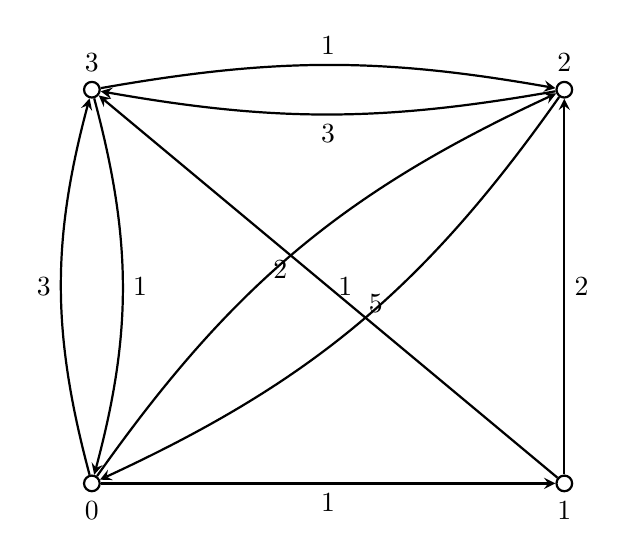
\begin{tikzpicture}
[nodedecorate/.style={shape=circle,inner sep=2pt,draw,thick},%
  arrowdecorate/.style={->,>=stealth,thick}]
% nodes or vertices
\node (0) at (0,0) [nodedecorate] {};
\node [below] at (0.south) {$0$};
\node (1) at (6,0) [nodedecorate] {};
\node [below] at (1.south) {$1$};
\node (2) at (6,5) [nodedecorate] {};
\node [above] at (2.north) {$2$};
\node (3) at (0,5) [nodedecorate] {};
\node [above] at (3.north) {$3$};
% edges or lines
\path
(0) edge[arrowdecorate] node[below]{$1$} (1)
(0) edge[arrowdecorate,bend left=15] node[below left]{$2$} (2)
(0) edge[arrowdecorate,bend left=15] node[left]{$3$} (3)
(1) edge[arrowdecorate] node[right]{$2$} (2)
(1) edge[arrowdecorate] node[right]{$1$} (3)
(2) edge[arrowdecorate,bend left=15] node[above right]{$5$} (0)
(2) edge[arrowdecorate,bend left=10] node[below]{$3$} (3)
(3) edge[arrowdecorate,bend left=15] node[right]{$1$} (0)
(3) edge[arrowdecorate,bend left=10] node[above]{$1$} (2);
\end{tikzpicture}
\caption{Demonstrating the Floyd-Roy-Warshall algorithm.}
\label{fig:graph_algorithms:Floyd_Roy_Warshall_demo}
\end{figure}
%sage: A = matrix([[0,1,2,3],[0,0,2,1],[-5,0,0,3],[1,0,1,0]])
%sage: D = DiGraph(A, format="weighted_adjacency_matrix")
%sage: D.plot(edge_labels=True, graph_border=True).show()

\begin{lstlisting}
sage: A = matrix([[0,1,2,3], [0,0,2,1], [-1/2,0,0,3], [1,0,1,0]]); A
sage: floyd_roy_warshall(A)
([[0, 1, 2, 2], [3/2, 0, 2, 1], [-1/2, 1/2, 0, 3/2], [1/2, 3/2, 1, 0]],
  [-1  1  2  1]
  [ 2 -1  2  3]
  [-1  0 -1  1]
  [ 2  2 -1 -1])
\end{lstlisting}

The plot of this weighted digraph with four vertices appears in
Figure~\ref{fig:graph_algorithms:another_Floyd_Roy_Warshall_demo}.

\begin{figure}[!htbp]
\centering
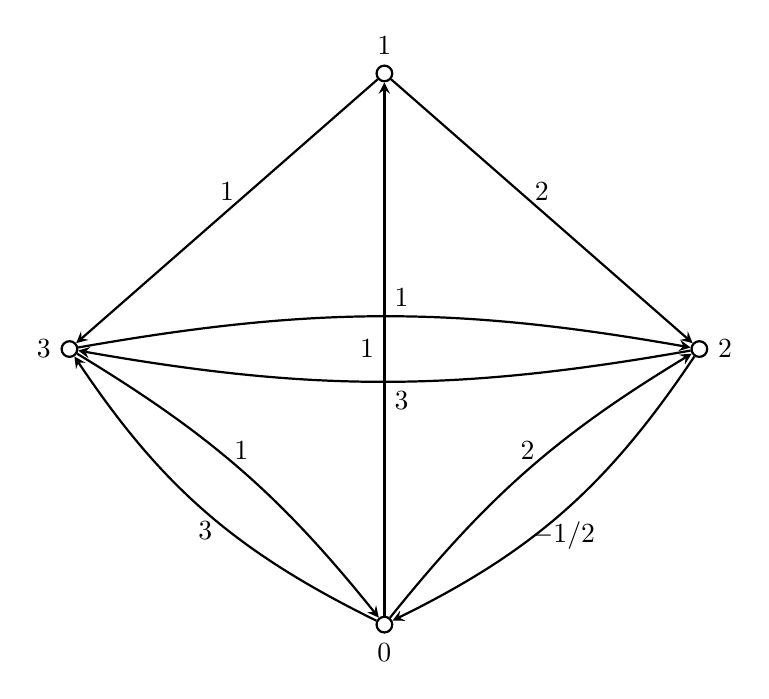
\begin{tikzpicture}
[nodedecorate/.style={shape=circle,inner sep=2pt,draw,thick},%
  arrowdecorate/.style={->,>=stealth,thick}]
% nodes or vertices
\node (0) at (0,0) [nodedecorate] {};
\node [below] at (0.south) {$0$};
\node (1) at (0,7) [nodedecorate] {};
\node [above] at (1.north) {$1$};
\node (2) at (4,3.5) [nodedecorate] {};
\node [right] at (2.east) {$2$};
\node (3) at (-4,3.5) [nodedecorate] {};
\node [left] at (3.west) {$3$};
% edges or lines
\path
(0) edge[arrowdecorate] node[left]{$1$} (1)
(0) edge[arrowdecorate,bend left=10] node[above]{$2$} (2)
(0) edge[arrowdecorate,bend left=15] node[below]{$3$} (3)
(1) edge[arrowdecorate] node[above]{$2$} (2)
(1) edge[arrowdecorate] node[above]{$1$} (3)
(2) edge[arrowdecorate,bend left=15] node[below]{$-1/2$} (0)
(2) edge[arrowdecorate,bend left=10] node[below right]{$3$} (3)
(3) edge[arrowdecorate,bend left=10] node[above]{$1$} (0)
(3) edge[arrowdecorate,bend left=10] node[above right]{$1$} (2);
\end{tikzpicture}
\caption{Another demonstration of the Floyd-Roy-Warshall algorithm.}
\label{fig:graph_algorithms:another_Floyd_Roy_Warshall_demo}
\end{figure}
%sage: A = matrix([[0,1,2,3],[0,0,2,1],[-1/2,0,0,3],[1,0,1,0]])
%sage: D = DiGraph(A, format="weighted_adjacency_matrix")
%sage: D.plot(edge_labels=True, graph_border=True).show()


%%%%%%%%%%%%%%%%%%%%%%%%%%%%%%%%%%%%%%%%%%%%%%%%%%%%%%%%%%%%%%%%%%%%%%%%%%%

\subsection{Transitive closure}

Consider a digraph $G = (V, E)$ of order $n = |V|$. The
\emph{transitive closure}\index{transitive closure} of $G$ is defined
as the digraph $G^* = (V, E^*)$ having the same vertex set as
$G$. However, the edge set $E^*$ of $G^*$ consists of all edges $uv$
such that there is a $u$-$v$ path in $G$ and $uv \notin E$. The
transitive closure $G^*$ answers an important question about $G$: If
$u$ and $v$ are two distinct vertices of $G$, are they connected by a
path with length $\geq 1$?

To compute the transitive closure of $G$, we let each edge of $G$ be
of unit weight and apply the Floyd-Roy-Warshall
Algorithm~\ref{alg:graph_algorithms:Floy_Roy_Warshall} on $G$. By
Corollary~\ref{cor:introduction:any_path_has_length_at_most_n_minus_1},
for any $i$-$j$ path in $G$ we have $D[i,j] < n$, and if there are no
paths from $i$ to $j$ in $G$, we have $D[i,j] = \infty$. This
procedure for computing transitive closure runs in time $O(n^3)$.

Modifying the Floyd-Roy-Warshall algorithm slightly, we obtain an
algorithm for computing transitive closure that, in practice, is more
efficient than Algorithm~\ref{alg:graph_algorithms:Floy_Roy_Warshall}
in terms of time and space. Instead of using the operations $\min$ and
$+$ as is the case in the Floyd-Roy-Warshall algorithm, we replace
these operations with the logical operations $\vee$~(logical \OR) and
$\wedge$~(logical \AND), respectively. For $i,j,k = 1, 2, \dots, n$,
define $T_k(i,j) = 1$ if there is an $i$-$j$ path in $G$ with all
intermediate vertices belonging to $\{1, 2, \dots, k\}$, and
$T_k(i,j) = 0$ otherwise. Thus, the edge $ij$ belongs to the
transitive closure $G^*$ if and only if $T_k(i,j) = 1$. The definition
of $T_k(i,j)$ can be cast in the form of a recursive definition as
follows. For $k = 0$, we have
\[
T_0(i,j)
=
\begin{cases}
0, & \text{if $i \neq j$ and $ij \notin E$}, \\
1, & \text{if $i = j$ or $ij \in E$}
\end{cases}
\]
and for $k > 0$, we have
\[
T_k(i,j)
=
T_{k-1}(i,j) \vee \big( T_{k-1}(i,k) \wedge T_{k-1}(k,j) \big).
\]
We need not use the subscript $k$ at all and instead let $T$ be a
boolean matrix such that $T[i,j] = 1$ if and only if there is an
$i$-$j$ path in $G$, and $T[i,j] = 0$ otherwise. Using the above
notations, the Floyd-Roy-Warshall algorithm is translated to
Algorithm~\ref{alg:graph_algorithms:Floy_Roy_Warshall:transitive_closure}
for obtaining the boolean matrix $T$. We can then use $T$ and the
definition of transitive closure to obtain the edge set $E^*$ in the
transitive closure $G^* = (V, E^*)$ of $G = (V, E)$.

A more efficient transitive closure algorithm can be found in the PhD
thesis of Esko Nuutila~\cite{Nuutila1995}. The transitive closure
algorithm as presented in
Algorithm~\ref{alg:graph_algorithms:Floy_Roy_Warshall:transitive_closure}
is due to Stephen Warshall~\cite{Warshall1962}. It is a special case
of a more general algorithm in automata theory due to Stephen
Kleene~\cite{Kleene1956}, called Kleene's algorithm.

\begin{algorithm}[!htpb]
\dontprintsemicolon  % no semicolon at end of pseudocode statements
%% data section
\SetKwInOut{Input}{Input}
\SetKwInOut{Output}{Output}
%% input/output
\Input{A digraph $G = (V, E)$ that has no self-loops. Vertices are
  numbered from 1 to $n$, i.e. $V = \{1, 2, \dots, n\}$.}
\Output{The boolean matrix $T$ such that $T[i,j] = 1$ if and only if
  there is an $i$-$j$ path in $G$, and $T[i,j] = 0$ otherwise.}
\BlankLine
%% algorithm body
$n \leftarrow |V|$\;
$T \leftarrow$ adjacency matrix of $G$\;
%% \For{$i \leftarrow 1, 2, \dots, n$}{
%%   \For{$j \leftarrow 1, 2, \dots, n$}{
%%     \eIf{$i = j$ \emph{or} $ij \in E$}{
%%       $T[i,j] \leftarrow 1$\;
%%     }{
%%       $T[i,j] \leftarrow 0$\;
%%     }
%%   }
%% }
\For{$k \leftarrow 1, 2, \dots, n$}{
  \For{$i \leftarrow 1, 2, \dots, n$}{
    \For{$j \leftarrow 1, 2, \dots, n$}{
      $T[i,j] \leftarrow T[i,j] \vee \big( T[i,k] \wedge T[k,j] \big)$\;
    }
  }
}
\Return $T$\;
\caption{Variant of the Floyd-Roy-Warshall algorithm for transitive closure.}
\label{alg:graph_algorithms:Floy_Roy_Warshall:transitive_closure}
\end{algorithm}


%%%%%%%%%%%%%%%%%%%%%%%%%%%%%%%%%%%%%%%%%%%%%%%%%%%%%%%%%%%%%%%%%%%%%%%%%%%

\section{Johnson's algorithm}

See section~25.3 of Cormen~et~al.~\cite{CormenEtAl2001} and
Johnson~\cite{Johnson1977}.

Let $G = (V,E)$ be a graph with edge weights but no negative cycles.
\emph{Johnson's algorithm} finds a shortest path between all pairs of
vertices in a ``sparse'' directed graph.
\index{Johnson's algorithm}

\begin{algorithm}[!htpb]
\dontprintsemicolon  % no semicolon at end of pseudocode statements
%% data section
\SetKwInOut{Input}{Input}
\SetKwInOut{Output}{Output}
\SetKwData{False}{False}
%% input/output
\Input{A sparse weighted digraph $G = (V, E)$, where the vertex set is
  $V = \{1, 2, \dots, n\}$.}
\Output{If $G$ has negative-weight cycles, then return
  \False. Otherwise, return an $n \times n$ matrix $D$ of shortest-path
  weights and a list $P$ such that $P[v]$ is a parent list resulting
  from running Dijkstra's algorithm on $G$ with start vertex $v$.}
\BlankLine
%% algorithm body
$s \leftarrow$ vertex not in $V$\;
$V' \leftarrow V \cup \{s\}$\;
$E' \leftarrow E \cup \{sv \;|\; v \in V\}$\;
$G' \leftarrow$ digraph $(V', E')$ with weight $w(sv) = 0$ for all $v \in V$\;
\If{$\BellmanFord(G', w, s) = \False$}{
  \Return \False\;
}
$d \leftarrow$ distance list returned by $\BellmanFord(G', w, s)$\;
\For{\emph{each edge} $uv \in E'$}{
  $\hat{w}(uv) \leftarrow w(uv) + d[u] - d[v]$\;
}
\For{\emph{each vertex} $u \in V$}{
  $(\hat{\delta}, \hat{P}) \leftarrow$ distance and parent lists returned by $\Dijkstra(G, \hat{w}, u)$\;
  $P[u] \leftarrow \hat{P}$\;
  \For{\emph{each vertex} $v \in V$}{
    $D[u,v] \leftarrow \hat{\delta}[v] + d[v] - d[u]$\;
  }
}
\Return $(D, P)$\;
\caption{Johnson's algorithm for sparse graphs.}
\label{alg:graph_algorithms:Johnson_algorithm}
\end{algorithm}

The time complexity, for sparse graphs, is
$O(|V|^2\log |V| + |V| \cdot |E)|=O(n^2\log n)$, where $n = |V|$ is
the number of vertices of the original graph $G$.


%%%%%%%%%%%%%%%%%%%%%%%%%%%%%%%%%%%%%%%%%%%%%%%%%%%%%%%%%%%%%%%%%%%%%%%%%%%

\section{Problems}

\begin{enumerate}
\item Let $G = (V, E)$ be an undirected graph, let $s \in V$, and $D$
  is the list of distances resulting from running
  Algorithm~\ref{alg:graph_algorithms:breadth_first_search_template}
  with $G$ and $s$ as input. Show that $G$ is connected if and only if
  $D[v]$ is defined for each $v \in V$.

\item Show that the worst-case time complexity of depth-first search
  Algorithm~\ref{alg:graph_algorithms:depth_first_search_template} is
  $O(|V| + |E|)$.

\item Let $D$ be the list of distances returned by
  Algorithm~\ref{alg:graph_algorithms:depth_first_search_template},
  let $s$ be a starting vertex, and let $v$ be a vertex such that
  $D[v] \neq \infty$. Show that $D[v]$ is the length of any shortest
  path from $s$ to $v$.

\item Consider the graph in
  Figure~\ref{fig:graph_algorithms:Dijkstra_algorithm_digraph} as
  undirected. Run this undirected version through Dijkstra's algorithm
  with starting vertex $v_1$.

\begin{figure}[!htbp]
\centering
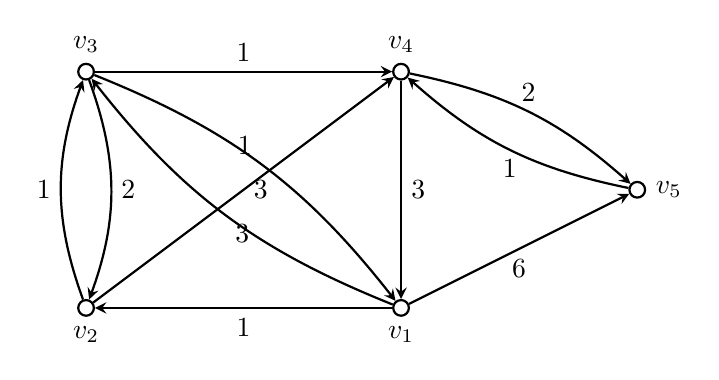
\begin{tikzpicture}
[nodedecorate/.style={shape=circle,inner sep=2pt,draw,thick},%
  arrowdecorate/.style={->,>=stealth,thick}]
%% nodes or vertices
\foreach \nodename/\x/\y/\direction/\navigate in {v_1/4/0/below/south,
  v_2/0/0/below/south, v_3/0/3/above/north, v_4/4/3/above/north,
  v_5/7/1.5/right/east} {
  \node (\nodename) at (\x,\y) [nodedecorate] {};
  \node [\direction] at (\nodename.\navigate) {$\nodename$};
}
%% edges or lines
\path
\foreach \startnode/\endnode/\direction/\weight in {v_1/v_2/below/1,
  v_1/v_5/below/6, v_2/v_4/right/3, v_3/v_4/above/1, v_4/v_1/right/3} {
  (\startnode) edge[arrowdecorate] node[\direction]{$\weight$} (\endnode)
}
\foreach \startnode/\endnode/\direction/\angle/\weight in {
  v_3/v_2/right/20/2, v_3/v_1/above left/15/1, v_2/v_3/left/20/1,
  v_1/v_3/below right/15/3, v_4/v_5/above/15/2, v_5/v_4/below/15/1} {
  (\startnode) edge[arrowdecorate,bend left=\angle] node[\direction]{$\weight$} (\endnode)
};
\end{tikzpicture}
\caption{Searching a directed house graph using Dijkstra's algorithm.}
\label{fig:graph_algorithms:Dijkstra_directed_house_graph}
\end{figure}
%sage: M = matrix([[0,1,3,0,6],[0,0,1,3,0],[1,2,0,1,0],[3,0,0,0,2],[0,0,0,1,0]])
%sage: D = DiGraph(M, format="weighted_adjacency_matrix")
%sage: D.plot(edge_labels=True, graph_border=True).show()

\item Consider the graph in
  Figure~\ref{fig:graph_algorithms:Dijkstra_directed_house_graph}. Choose
  any vertex as a starting vertex and run Dijkstra's algorithm over
  it. Now consider the undirected version of that digraph and repeat
  the exercise.
\end{enumerate}

%%-----------------------------------------------------------------------%%
%%--- Trees and Forests -------------------------------------------------%%

\chapter{Trees and Forests}
\label{chap:trees_forests}

In section~\ref{subsec:introduction:walks_trails_paths}, we briefly
touched upon trees and provided examples of how trees could be used to
model hierarchical structures. This chapter provides an in-depth study
of trees, their properties, and various applications.

{\color{red}{
\begin{itemize}
\item Discuss heaps and how these relate to realizing efficient
  implementations of Dijkstra's
  Algorithm~\ref{alg:graph_algorithms:dijkstra_general}.
\end{itemize}
}
}


%%-----------------------------------------------------------------------%%
%%--- Definitions and examples ------------------------------------------%%

\section{Definitions and examples}

Recall that a path in a graph $G = (V, E)$ whose start and end vertices
are the same is called a cycle. We say $G$ is
\emph{acyclic}\index{acyclic}, or a \emph{forest}\index{forest}, if it
has no cycles. In a forest, a vertex of degree one is called an
\emph{endpoint}\index{endpoint} or a \emph{leaf}\index{leaf}. A
connected forest is a \emph{tree}\index{tree}.

A \emph{rooted tree}\index{tree!rooted} is a tree with a specified
\emph{root}\index{root} vertex $v_0$. (However, if $G$ is a rooted
tree with root vertex $v_0$ having degree one then, by convention, we
do not call $v_0$ an endpoint or a leaf.) The Unix\index{Unix}, in
particular Linux\index{Linux}, filesystem\index{filesystem} hierarchy
can be viewed as a tree~(see
Figure~\ref{fig:trees_forests:filesystem_hierarchy}). As shown in
Figure~\ref{fig:trees_forests:filesystem_hierarchy}, the root vertex
is designated with the forward slash, which is also referred to as the
root directory\index{root directory}.

\begin{figure}[!htbp]
\centering
\begin{tikzpicture}
\node {\texttt{/}} [edge from parent fork down]
  child {node {\texttt{bin}}}
  child {node {\texttt{etc}}}
  child {node {\texttt{home}}
    child {node {\texttt{anne}}}
    child {node {\texttt{sam}}}
    child {node {$\dots$}}
  }
  child {node {\texttt{lib}}}
  child {node {\texttt{opt}}}
  child {node {\texttt{proc}}}
  child {node {\texttt{tmp}}}
  child {node {\texttt{usr}}
    child {node {\texttt{bin}}
      child {node {\texttt{acyclic}}}
      child {node {\texttt{diff}}}
      child {node {\texttt{dot}}}
      child {node {\texttt{gc}}}
      child {node {\texttt{neato}}}
      child {node {$\dots$}}
    }
    child {node {\texttt{include}}}
    child {node {\texttt{local}}}
    child {node {\texttt{share}}}
    child {node {\texttt{src}}}
    child {node {$\dots$}}
  }
  child {node {$\dots$}};
\end{tikzpicture}
\caption{The Linux filesystem hierarchy.}
\label{fig:trees_forests:filesystem_hierarchy}
\end{figure}

A \emph{directed tree}\index{tree!directed} is a digraph which would
be a tree if the directions on the edges were ignored. A rooted tree
can be regarded as a directed tree since we can imagine an edge
$E = uv$ for $u,v \in V$ being directed from $u$ to $v$ if and only
if $v$ is further away from $v_0$ than $u$ is. If $e = uv$ is an edge
in a rooted tree, then we call $v$ a \emph{child}\index{child} vertex
with \emph{parent}\index{parent} $u$. Directed trees are pervasive in
theoretical computer science, as they are useful structures for
describing algorithms and relationships between objects in certain
data sets.

An \emph{ordered tree}\index{tree!ordered} is a rooted tree for which
an ordering is specified for the children of each vertex. An
$n$-\emph{ary tree}\index{tree!$n$-ary} is a rooted tree for which
each vertex that is not a leaf has at most $n$ children. The case
$n = 2$ are called \emph{binary trees}\index{tree!binary}. A
\emph{spanning tree}\index{spanning tree} $T$ of a connected,
undirected graph $G$ is a subgraph containing all vertices of $G$
which is a tree.

\begin{example}
\label{example:span-tree}
{\rm
Consider the $4 \times 4$ grid graph with $16$ vertices and
$24$ edges. Two examples of a spanning tree are given in
Figure~\ref{fig:trees_forests:grid_graph_spanning_trees} by using
thicker line width for its edges.}
\hfill $\square$
\end{example}

\begin{figure}[!htbp]
\centering
\subfigure[]{
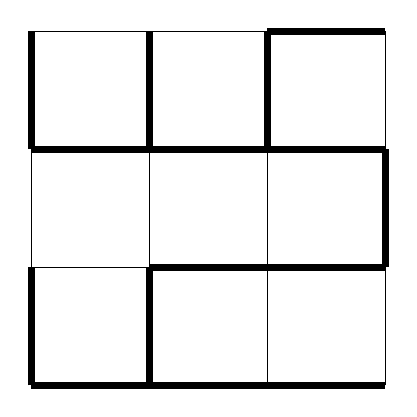
\begin{tikzpicture}
[linedecorate/.style={line width=2.5pt}]
%% set up the grid
\foreach \xstart/\xend/\y in {0/4.5/0, 0/4.5/1.5, 0/4.5/3, 0/4.5/4.5} {
  \draw (\xstart,\y) -- (\xend,\y);
  \draw (\y,\xstart) -- (\y,\xend);
}
%% draw the spanning tree
\foreach \xstart/\ystart/\xend/\yend in {0/0/0/1.5, 0/0/4.5/0,
  1.5/0/1.5/1.5, 1.5/1.5/4.5/1.5, 4.5/1.5/4.5/3, 0/3/4.5/3, 0/3/0/4.5,
  1.5/3/1.5/4.5, 3/3/3/4.5, 3/4.5/4.5/4.5} {
  \draw[linedecorate] (\xstart,\ystart) -- (\xend,\yend);
}
\end{tikzpicture}
}
%%
%%
\qquad
\subfigure[]{
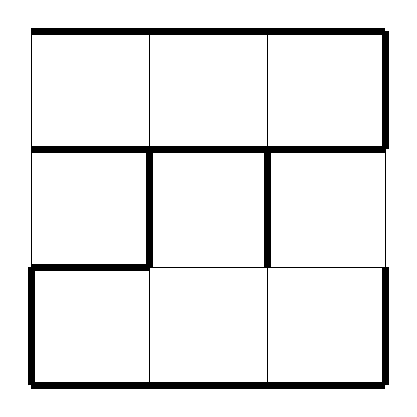
\begin{tikzpicture}
[linedecorate/.style={line width=2.5pt}]
\foreach \xstart/\xend/\y in {0/4.5/0, 0/4.5/1.5, 0/4.5/3, 0/4.5/4.5} {
  \draw (\xstart,\y) -- (\xend,\y);
  \draw (\y,\xstart) -- (\y,\xend);
}
%% draw the spanning tree
\foreach \xstart/\ystart/\xend/\yend in {0/0/0/1.5, 0/0/4.5/0,
  4.5/0/4.5/1.5, 0/1.5/1.5/1.5, 1.5/1.5/1.5/3, 3/1.5/3/3, 0/3/4.5/3,
  4.5/3/4.5/4.5, 0/4.5/4.5/4.5} {
  \draw[linedecorate] (\xstart,\ystart) -- (\xend,\yend);
}
\end{tikzpicture}
}
\caption{Spanning trees for the $4 \times 4$ grid graph.}
\label{fig:trees_forests:grid_graph_spanning_trees}
\end{figure}

The following game is a variant of the Shannon switching game, due to
Edmunds and Lehman\index{edge-tagging game}. We follow the description
in Oxley's survey ({\it What is a matroid?'}
{\color{red}{add reference later}}). Recall that a minimal edge cut of
a graph is also called a bond\index{bond} of the graph. The following
two-person game is played on a connected graph $G = (V,E)$. Two
players Alice and Bob alternately tag elements of $E$. Alice's goal is
to tag the edges of a spanning tree, while Bob's goal is to tag the
edges of a bond. If we think of this game in terms of a communication
network, then Bob's goal is to separate the network into pieces that
are no longer connected to each other, while Alice is aiming to
reinforce edges of the network to prevent their destruction. Each move
for Bob consists of destroying one edge, while each move for Alice
involves securing an edge against destruction.

\begin{theorem}
The following statements are equivalent for a connected graph $G$.
%
\begin{enumerate}
\item Bob plays first and Alice can win against all possible
  strategies of Bob.

\item The graph $G$ has 2 edge-disjoint spanning trees.

\item For all partitions $P$ of the vertex set $V$ of $G$, the number
  of edges of $G$ that join vertices in different classes of the
  partition is at least $2(|P| - 1)$.
\end{enumerate}
\end{theorem}

%%-----------------------------------------------------------------------%%
%%--- Properties of trees -----------------------------------------------%%

\section{Properties of trees}

%\begin{itemize}
%\item trees and acyclic graphs; leaves
%
%\item forests
%\end{itemize}

The following theorem gives several basic
characterizations of trees.

\begin{theorem}
If $T = (V, E)$ is a graph with $n$ vertices, then the following
statements are equivalent:
\begin{enumerate}
\item $T$ is a tree.

\item $T$ contains no cycles and has $n - 1$ edges.

\item $T$ is connected and has $n - 1$ edges.

\item Every edge of $T$ is a cut set.

\item For any $u,v \in V$, there is exactly one $u$-$v$ path.

\item For any new edge $e$, the join $T + e$ has exactly one cycle.
\end{enumerate}
\end{theorem}

Let $G=(V_1,E_2)$ be a graph and $T=(V_2,E_2)$ a subgraph of $G$ which is a tree.
As in (6) we see adding just one edge in $E_1-E_2$ to $T$ will create a
unique cycle in $G$. Such a cycle is called a {\it fundamental cycle}
of $G$. (The set of such fundamental cycles of $G$ depends on $T$.)
\index{fundamental cycle}
\index{tree}

\begin{proof}[Solution]
\noindent
(1) $\implies$ (2):
This basically follows by induction on the number of vertices.

By definition, a tree has no cycles. Make the following
induction hypothesis: for any tree $T=(V,E)$, $|E|=|V|-1$.
This holds in the base case where $|V|=1$ since in that case,
there can be no edges. Assume it is true for all trees with
$|V|=k$, for some $k>1$. Let $T=(V,E)$ be a tree having
$k+1$ vertices. Remove an edge (but not the vertices
it is incident to). This
disconnects
$T$ into $T_1=(V_1, E_1)$ union $T_2 = (V_2, E_2)$,
where $|E|=|E_1|+|E_2|+1$ and $|V|=|V_1|+|V_2|$
(and possibly one of the $E_i$ is empty),
each of which is a tree satisfying the conditions of the induction
hypothesis. Therefore,

\[
|E|=|E_1|+|E_2|+1 = |V_1| - 1 + |V_2| - 1 + 1 =|V|-1.
\]

\noindent
(2) $\implies$ (3):
If $T=(V,E)$ has $k$ connected components then it is a disjoint
union of trees $T_i=(V_i,E_i)$, $i=1,2,\dots, k$,
for some $k$. Each of these satisfy, by (2),

\[
|E_i|=|V_i|-1,
\]
so

\[
|E|=\sum_{i=1}^k |E_i|
=\sum_{i=1}^k |V_i| -k
=|V|-k.
\]
This contradicts (2) unless $k=1$.
Therefore, $T$ is connected.

\noindent
(3) $\implies$ (4):
If removing an edge $e\in E$ leaves $T=(V,E)$ connected then
$T'=(V,E')$ is a tree, where $E'=E-e$.
However, this means that $|E'|=|E|-1=|V|-1-1=|V|-2$,
which contradicts (3). Therefore $e$ is a cut set.

\noindent
(4) $\implies$ (5):
Let

\[
P = (v_0=u\to v_1 \to v_2 \to \dots \to v_k = v)
\]
and
\[
P' = (v'_0=u\to v'_1 \to v'_2 \to \dots \to v'_\ell = v)
\]
be two paths from $u$ to $v$.

\noindent
(5) $\implies$ (6):
Let $e=(u,v)$ be a new edge connecting $u,v\in V$.
Suppose that

\[
P = (v_0=w\to v_1 \to v_2 \to \dots \to v_k = w)
\]
and
\[
P' = (v'_0=w\to v'_1 \to v'_2 \to \dots \to v'_\ell = w)
\]
are two cycles in $T\cup (\{u,v\},\{e\})$.

If either $P$ or $P'$ does not contain $e$,
say $P$ does not contain $e$, then $P$ is a
cycle in $T$. Let $u = v_0$ and let $v=v_1$.
The edge $v_0=w\to v_1$ is a $u$-$v$ path
and the sequence $v=v_1 \to v_2 \to \dots \to v_k=w=u$
taken in reverse order is another $u$-$v$ path.
This is a contradiction to (5).

We may suppose now that $P$ and $P'$ both contain $e$.
Therefore, $P$ contains a subpath $P_0=P-e$ (which is not
closed), that is the same as $P$ except it lacks the edge
from $u$ to $v$. Likewise, $P'$ contains a subpath $P'_0=P'-e$ (which is not
closed), that is the same as $P'$ except it lacks the edge
from $u$ to $v$. By (5), these $u$-$v$ paths
$p_0$ and $P_0'$ must be the same. This forces
$P$ and $P'$ to be the same, which proves (6).


\noindent
(6) $\implies$ (1):
Condition (6) implies that $T$ is acyclic. (Otherwise, it is trivial
to make two cycles by adding an extra edge.) We must show $T$ is connected.
Suppose $T$ is disconnected. Let $u$ be a vertex in one component,
$T_1$ say,
of $T$ and $v$ a vertex in another component, $T_2$ say, of $T$.
Adding the edge $e=(u,v)$ does not create a cycle (if it did
then $T_1$ and $T_2$ would not be disjoint), which contradicts (6).
\end{proof}

\begin{exercise}
Let $G=(V_1,E_2)$ be a graph and $T=(V_2,E_2)$ a spanning tree of $G$.
Show there is a one-to-one correspondence between fundamental cycles in $G$ and
edges not in $T$.
\end{exercise}

\begin{exercise}
Let $G=(V, E)$ be the $3\times 3$ grid graph and $T_1=(V_1,E_1)$,
$T_2=(V_2,E_2)$ be spanning trees of $G$ in Example \ref{example:span-tree}.
Find a fundamental cycle in $G$ for $T_1$ which is not a
fundamental cycle in $G$ for $T_2$.
\end{exercise}

\begin{exercise}
Usually there exist many spanning trees of a graph.
Can you classify those graphs for which there is only one spanning tree?
In other words, find necessary and sufficient conditions for a
graph $G$ such that if $T$ is a spanning tree then $T$ is unique.
\end{exercise}


%%-----------------------------------------------------------------------%%
%%--- Minimum spanning trees --------------------------------------------%%

\section{Minimum spanning trees}

Suppose you want to design an electronic circuit
connecting several components. If these components represent the
vertices of the graph and a wire connecting two components
represents an edge of the graph then, for economical reasons, you will want to
connect these together using the least amount of wire.
This amounts to finding a minimum spanning tree in the
complete graph on these vertices.

\begin{itemize}
\item spanning trees

We can characterize a spanning tree in several ways. Each of these
conditions lead to an algorithm for constructing them.

One condition is that spanning tree of a connected graph $G$ can also
be defined as a maximal set of edges of $G$ that contains no cycle.
Another condition is that it is a minimal set of edges that connect
all vertices.

Exploiting the former criteria gives rise to Kruskal's algorithm.
Exploiting the latter criteria gives rise to Prim's algorithm.
Both of these argorithms are discussed in more detail below.

\item minimum-cost spanning trees

A {\it minimum spanning tree} (MST) is a spanning
tree of an edge weighted graph having lowest total weight
among all possible spanning trees.
\index{tree!minimum spanning}
\index{MST}

\item Kruskal's algorithm~\cite{Kruskal1956}; see also section~23.2 of
  Cormen~et~al.~\cite{CormenEtAl2001}.

Kruskal's algorithm is a greedy algorithm to compute a MST.
It was discovered by J. Kruskal in the 1950's.

Kruskal's algorithm can be shown to run in $O(|E| \log |E|)$ time.


\item Prim's algorithm~\cite{Prim1957}; see also section~23.2 of
  Cormen~et~al.~\cite{CormenEtAl2001}.

Prim's algorithm is a greedy algorithm to compute a MST. In can be
implemented in time $O(|E| + |V| \log |V|)$, which is
$O(n^2)$ for a dense graph having $n$ vertices.

The algorithm was developed in the 1930's by Czech mathematician V.
Jarn\'ik and later independently by both the computer scientists R. Prim
and E. Dijkstra in the 1950's.

\item Bor\r{u}vka's algorithm~\cite{Boruvka1926a,Boruvka1926b}

Bor\r{u}vka's algorithm is an algorithm for finding a minimum spanning
tree in a graph
for which all edge weights are distinct.
It was first published in 1926 by Otakar Bor\o uvka but then
rediscovered by many others.

Bor\r{u}vka's algorithm can be shown to run in time
$O(|E|\log |V|)$.


\end{itemize}

\subsection{Kruskal's algorithm}

Kruskal's algorithm starts with an edge-weighted digraph $G=(V,E)$
as input. Let $w:E\to {\mathbb{R}}$ denote the weight function.
The first stage is to create a ``skeleton'' of the
tree $T$ which is initially set to be a graph with no
edges: $T=(V,\emptyset)$. The next stage is to
sort the edges of $G$ by weight. In other words, we
label the edges of $G$ as

\[
E = \{e_1,e_2,\dots ,e_m\},
\]
where $w(e_1) \leq w(e_2) \leq \dots \leq w(e_m)$.
Next, start a for loop over $e\in E$. You add
$e$ to $T$ as an edge provided it does not create
a cycle. The only way adding $e=(u,v)$ to $T$ would
create a cycle would be if both $u$ and $v$ were
endpoints of an edge already in $T$. As long as this
cycle condition fails, you add $e$ to $T$ and otherwise,
go to the next element of $E$ in the for loop.
At the end of the for loop, the edges of $T$ have
been completely found and the algorithm stops.

\begin{center}
\vskip .15in

\begin{Verbatim}[fontsize=\scriptsize,fontfamily=courier,fontshape=tt,frame=single,label=\sage]

def kruskal(G):
    """
    Implements Kruskal's algorithm to compute a MST of a graph.

    INPUT:
        G - a connected edge-weighted graph or digraph
               whose vertices are assumed to be 0, 1, ...., n-1.
    OUTPUT:
        T - a minimum weight spanning tree.

    If G is not explicitly edge-weighted then the algorithm
    assumes all edge weights are 1. The tree T returned is
    a weighted graph, even if G is not.

    EXAMPLES:
        sage: A = matrix([[0,1,2,3],[0,0,2,1],[0,0,0,3],[0,0,0,0]])
        sage: G = DiGraph(A, format = "adjacency_matrix", weighted = True)
        sage: TE = kruskal(G); TE.edges()
        [(0, 1, 1), (0, 2, 2), (1, 3, 1)]
        sage: G.edges()
        [(0, 1, 1), (0, 2, 2), (0, 3, 3), (1, 2, 2), (1, 3, 1), (2, 3, 3)]
        sage: G = graphs.PetersenGraph()
        sage: TE = kruskal(G); TE.edges()
        [(0, 1, 1), (0, 4, 1), (0, 5, 1), (1, 2, 1), (1, 6, 1), (2, 3, 1),
         (2, 7, 1), (3, 8, 1), (4, 9, 1)]

    TODO:
        Add ''verbose'' option to make steps more transparent.
       (Useful for teachers and students.)
    """
    T_vertices = G.vertices() # a list of the form range(n)
    T_edges = []
    E = G.edges() # a list of triples
    # start ugly hack
    Er = [list(x) for x in E]
    E0 = []
    for x in Er:
        x.reverse()
        E0.append(x)
    E0.sort()
    E = []
    for x in E0:
        x.reverse()
        E.append(tuple(x))
    # end ugly hack to get E is sorted by weight
    for x in E:  # find edges of T
        TV = flatten(T_edges)
        u = x[0]
        v = x[1]
        if not(u in TV and v in TV):
            T_edges.append([u,v])
    # find adj mat of T
    if G.weighted():
        AG = G.weighted_adjacency_matrix()
    else:
        AG = G.adjacency_matrix()
    GV = G.vertices()
    n = len(GV)
    AT = []
    for i in GV:
        rw = [0]*n
        for j in GV:
            if [i,j] in T_edges:
                rw[j] = AG[i][j]
        AT.append(rw)
    AT = matrix(AT)
    return Graph(AT, format = "adjacency_matrix", weighted = True)

\end{Verbatim}

\end{center}
\index{Kruskal's algorithm}

Here are some examples.

We start with the grid graph. This is implemented in Sage
in a way that the vertices are given by the coordinates of the
grid the graph lies on, as opposed to $0,1,\dots,n-1$.
Since the above implementation assumes that the
vertices are $V=\{0,1,\dots,n-1\}$, we first redefine
the graph suitable and run the Kruskal algorithm on that.

\begin{center}
\fontsize{9pt}{9pt}
\selectfont
\tt
\begin{lstlisting}
sage: G = graphs.GridGraph([4,4])
sage: A = G.adjacency_matrix()
sage: G = Graph(A, format = "adjacency_matrix", weighted = True)
sage: T = kruskal(G); T.edges()
[(0, 1, 1), (0, 4, 1), (1, 2, 1), (1, 5, 1), (2, 3, 1), (2, 6, 1), (3,7, 1),
 (4, 8, 1), (5, 9, 1), (6, 10, 1), (7, 11, 1), (8, 12, 1), (9, 13, 1),
 (10, 14, 1), (11, 15, 1)]
\end{lstlisting}
\end{center}
%
The plot of this graph is given in
Figure~\ref{fig:trees-forests:Kruskal_example}.


\begin{figure}[h!]
\begin{center}
\unitlength=0.920000pt
\begin{picture}(210.00,192.00)(0.00,0.00)
%\put(-3.00,-3.00){$\bullet$} % vertices look funny
%\put(-3.00,189.00){$\bullet$}
%\put(61.00,189.00){$\bullet$}

\thinlines
\put(0.00,192.00){\line(1,0){192.00}} %outer box
\put(192.00,0.00){\line(0,1){192.00}} %outer box
\put(0.00,0.00){\line(1,0){192.00}} %outer box
\put(0.00,0.00){\line(0,1){192.00}} %outer box

\put(0.00,64.00){\line(1,0){192.00}} %inner lines
\put(0.00,128.00){\line(1,0){192.00}} %inner lines

\put(64.00,0.00){\line(0,1){192.00}} %inner lines
\put(128.00,0.00){\line(0,1){192.00}} %inner lines

\linethickness{0.9mm}  % tree edges
\put(0.00,0.00){\line(0,1){192.00}}
\put(0.00,0.00){\line(1,0){192.00}}
\put(0.00,64.00){\line(1,0){192.00}}
\put(0.00,128.00){\line(1,0){192.00}}
\put(0.00,192.00){\line(1,0){192.00}}
\end{picture}
\end{center}
\label{fig:trees-forests:Kruskal_example}

\caption{Kruskal's algorithm for the $4\times 4$ grid graph.}
\end{figure}

\subsection{Prim's algorithm}

Prim's algorithm is an algorithm that finds a minimum spanning tree
for a connected weighted
undirected graph $\Gamma=(V,E)$. It is very similar to Kruskal's
algorithm except that it starts with an empty vertex set, rather than
a full one.



\begin{algorithm}[!htpb]
\dontprintsemicolon  % no semicolon at end of pseudocode statements
%% data section
\SetKwInOut{Input}{Input}
\SetKwInOut{Output}{Output}
\SetKwData{Count}{count}
\SetKwData{False}{False}
\SetKwData{True}{True}
%% input/output
\Input{A connected graph $G = (V, E)$ having edge weights. }
\Output{A MST $T$ for $G$.}
\BlankLine
%% algorithm body
Initialize: $V(T) = \{v_0\}$, where $v_0$ is an arbitrary vertex, $E(T)=\emptyset$ \;

While $V(T)\not= V$:\;
{
\quad Choose edge $(u,v)$ with minimal weight such that $u$ is in $V(T)$
but $v$ is not,\;
\quad Add $v$ to $V(T)$, add $(u, v)$ to $E(T)$.\;
}

\caption{Prim's algorithm.}
\label{alg:tree-forest:prim}
\end{algorithm}
\index{Prim's algorithm}

\begin{center}
\vskip .15in

\begin{Verbatim}[fontsize=\scriptsize,fontfamily=courier,fontshape=tt,frame=single,label=\sage]

def prim(G):
    """
    Implements Prim's algorithm to compute a MST of a graph.

    INPUT:
        G - a connected graph.
    OUTPUT:
        T - a minimum weight spanning tree.

    REFERENCES:
        http://en.wikipedia.org/wiki/Prim's_algorithm
    """
    T_vertices = [0] # assumes G.vertices = range(n)
    T_edges = []
    E = G.edges() # a list of triples
    V = G.vertices()
    # start ugly hack to sort E
    Er = [list(x) for x in E]
    E0 = []
    for x in Er:
        x.reverse()
        E0.append(x)
    E0.sort()
    E = []
    for x in E0:
        x.reverse()
        E.append(tuple(x))
    # end ugly hack to get E is sorted by weight
    for x in E:
        u = x[0]
        v = x[1]
        if u in T_vertices and not(v in T_vertices):
            T_edges.append([u,v])
            T_vertices.append(v)
    # found T_vertices, T_edges
    # find adj mat of T
    if G.weighted():
        AG = G.weighted_adjacency_matrix()
    else:
        AG = G.adjacency_matrix()
    GV = G.vertices()
    n = len(GV)
    AT = []
    for i in GV:
        rw = [0]*n
        for j in GV:
            if [i,j] in T_edges:
                rw[j] = AG[i][j]
        AT.append(rw)
    AT = matrix(AT)
    return Graph(AT, format = "adjacency_matrix", weighted = True)

\end{Verbatim}

\end{center}



\begin{center}
\fontsize{9pt}{9pt}
\selectfont
\tt
\begin{lstlisting}
        sage: A = matrix([[0,1,2,3],[3,0,2,1],[2,1,0,3],[1,1,1,0]])
        sage: G = DiGraph(A, format = "adjacency_matrix", weighted = True)
        sage: E = G.edges(); E
        [(0, 1, 1), (0, 2, 2), (0, 3, 3), (1, 0, 3), (1, 2, 2), (1, 3, 1), (2, 0, 2),
         (2, 1, 1), (2, 3, 3), (3, 0, 1), (3, 1, 1), (3, 2, 1)]
        sage: prim(G)
        Multi-graph on 4 vertices
        sage: prim(G).edges()
        [(0, 1, 1), (0, 2, 2), (1, 3, 1)]
\end{lstlisting}
\end{center}
%


\begin{figure}[!htbp]
\centering
\subfigure[]{
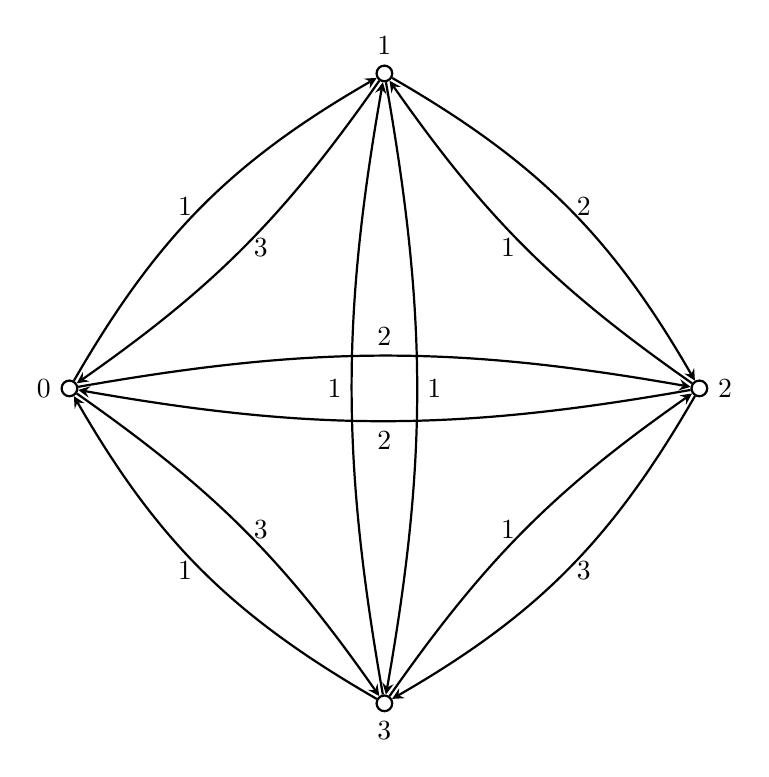
\begin{tikzpicture}
[nodedecorate/.style={shape=circle,inner sep=2pt,draw,thick},%
  arrowdecorate/.style={->,>=stealth,thick}]
% nodes or vertices
\node (0) at (-4,4) [nodedecorate] {};
\node [left] at (0.west) {$0$};
\node (1) at (0,8) [nodedecorate] {};
\node [above] at (1.north) {$1$};
\node (2) at (4,4) [nodedecorate] {};
\node [right] at (2.east) {$2$};
\node (3) at (0,0) [nodedecorate] {};
\node [below] at (3.south) {$3$};
% edges or lines
\path
(0) edge[arrowdecorate,bend left=15] node[left]{$1$} (1)
(0) edge[arrowdecorate,bend left=10] node[above]{$2$} (2)
(0) edge[arrowdecorate,bend left=10] node[right]{$3$} (3)
(1) edge[arrowdecorate,bend left=10] node[right]{$3$} (0)
(1) edge[arrowdecorate,bend left=15] node[right]{$2$} (2)
(1) edge[arrowdecorate,bend left=10] node[right]{$1$} (3)
(2) edge[arrowdecorate,bend left=10] node[below]{$2$} (0)
(2) edge[arrowdecorate,bend left=10] node[left]{$1$} (1)
(2) edge[arrowdecorate,bend left=15] node[right]{$3$} (3)
(3) edge[arrowdecorate,bend left=15] node[left]{$1$} (0)
(3) edge[arrowdecorate,bend left=10] node[left]{$1$} (1)
(3) edge[arrowdecorate,bend left=10] node[left]{$1$} (2);
\end{tikzpicture}
}
\subfigure[]{
\begin{tikzpicture}
[nodedecorate/.style={shape=circle,inner sep=2pt,draw,thick},%
  linedecorate/.style={-,thick}]
% nodes or vertices
\node (0) at (4,-4) [nodedecorate] {};
\node [right] at (0.east) {$0$};
\node (1) at (2,-2) [nodedecorate] {};
\node [right] at (1.east) {$1$};
\node (2) at (6,-6) [nodedecorate] {};
\node [right] at (2.east) {$2$};
\node (3) at (0,0) [nodedecorate] {};
\node [right] at (3.east) {$3$};
% edges or lines
\path
(3) edge[linedecorate] node[left]{$1$} (1)
(1) edge[linedecorate] node[left]{$1$} (0)
(0) edge[linedecorate] node[left]{$2$} (2);
\end{tikzpicture}
}
\caption{Prim's algorithm for digraphs. Above is the original digraph
  and below is the MST produced by Prim's algorithm.}
\label{fig:tree-forests:Prim_algorithm_digraph}
\end{figure}



\begin{center}
\fontsize{9pt}{9pt}
\selectfont
\tt
\begin{lstlisting}
        sage: A = matrix([[0,7,0,5,0,0,0],[0,0,8,9,7,0,0],[0,0,0,0,5,0,0],
         [0,0,0,0,15,6,0],[0,0,0,0,0,8,9],[0,0,0,0,0,0,11],[0,0,0,0,0,0,0]])
        sage: G = Graph(A, format = "adjacency_matrix", weighted = True)
        sage: E = G.edges(); E
        [(0, 1, 7), (0, 3, 5), (1, 2, 8), (1, 3, 9), (1, 4, 7), (2, 4, 5),
         (3, 4, 15), (3, 5, 6), (4, 5, 8), (4, 6, 9), (5, 6, 11)]
        sage: prim(G).edges()
        [(0, 1, 7), (0, 3, 5), (1, 2, 8), (1, 4, 7), (3, 5, 6), (4, 6, 9)]
\end{lstlisting}
\end{center}
%


\begin{figure}[!htbp]
\centering
\subfigure[]{
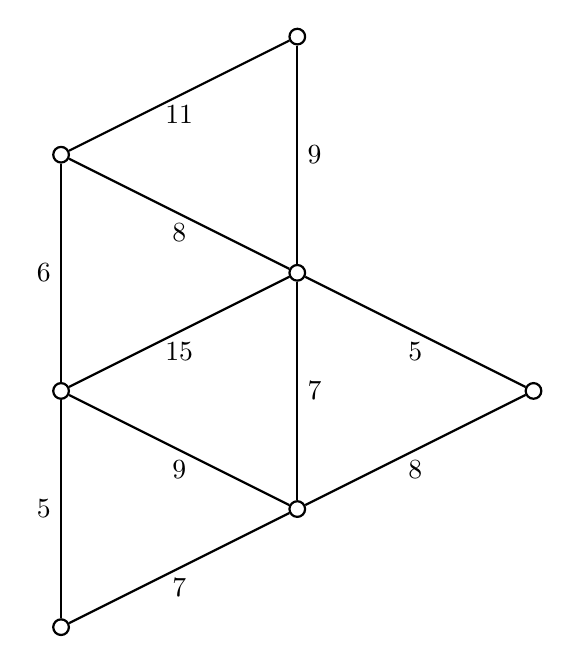
\begin{tikzpicture}
[nodedecorate/.style={shape=circle,inner sep=2pt,draw,thick},%
  linedecorate/.style={-,thick}]
% nodes or vertices
\node (0) at (0,0) [nodedecorate] {};
\node (1) at (3,1.5) [nodedecorate] {};
\node (2) at (6,3) [nodedecorate] {};
\node (3) at (0,3) [nodedecorate] {};
\node (4) at (3,4.5) [nodedecorate] {};
\node (5) at (0,6) [nodedecorate] {};
\node (6) at (3,7.5) [nodedecorate] {};
% edges or lines
\path
(0) edge[linedecorate] node[below]{$7$} (1)
(0) edge[linedecorate] node[left]{$5$} (3)
(1) edge[linedecorate] node[below]{$8$} (2)
(1) edge[linedecorate] node[below]{$9$} (3)
(1) edge[linedecorate] node[right]{$7$} (4)
(2) edge[linedecorate] node[below]{$5$} (4)
(3) edge[linedecorate] node[below]{$15$} (4)
(3) edge[linedecorate] node[left]{$6$} (5)
(4) edge[linedecorate] node[below]{$8$} (5)
(4) edge[linedecorate] node[right]{$9$} (6)
(5) edge[linedecorate] node[below]{$11$} (6);
\end{tikzpicture}
}
\subfigure[]{
\begin{tikzpicture}
[nodedecorate/.style={shape=circle,inner sep=2pt,draw,thick},%
  linedecorate/.style={-,thick}]
% nodes or vertices
\node (6) at (0,0) [nodedecorate] {};
\node [left] at (6.west) {$6$};
\node (4) at (2,2) [nodedecorate] {};
\node [left] at (4.west) {$4$};
\node (1) at (4,4) [nodedecorate] {};
\node [left] at (1.west) {$1$};
\node (2) at (6,2) [nodedecorate] {};
\node [left] at (2.west) {$2$};
\node (0) at (4,6) [nodedecorate] {};
\node [left] at (0.west) {$0$};
\node (3) at (4,8) [nodedecorate] {};
\node [left] at (3.west) {$3$};
\node (5) at (4,10) [nodedecorate] {};
\node [left] at (5.west) {$5$};
% edges or lines
\path
(6) edge[linedecorate] node[below]{$9$} (4)
(4) edge[linedecorate] node[below]{$7$} (1)
(1) edge[linedecorate] node[above]{$8$} (2)
(1) edge[linedecorate] node[right]{$7$} (0)
(0) edge[linedecorate] node[right]{$5$} (3)
(3) edge[linedecorate] node[right]{$6$} (5);
\end{tikzpicture}
}
\caption{Another example of Prim's algorithm. On the left is the
  original graph. On the right is the MST produced by Prim's algorithm.}
\label{fig:tree-forests:Prim_algorithm_digraph2}
\end{figure}


\subsection{Bor\r{u}vka's algorithm}

Bor\r{u}vka's algorithm algorithm is an algorithm
for finding a minimum spanning tree in a connected graph for
which all edge weights are distinct.
\index{Bor\r{u}vka's algorithm}

Pseudocode for Bor\r{u}vka's algorithm is:

\begin{itemize}
\item
Begin with a connected graph G containing edges of distinct
 weights, and an empty set of edges T
\item
While the vertices of G connected by T are disjoint:
\begin{itemize}
\item
Begin with an empty set of edges E
\item
         For each component:
\begin{itemize}
\item
        Begin with an empty set of edges S
\item
        For each vertex in the component:
 \begin{itemize}
\item
Add the cheapest edge from the vertex in
             the component to another vertex in a disjoint component to S
\end{itemize}
        Add the cheapest edge in S to E
\end{itemize}
    Add the resulting set of edges E to T.
\end{itemize}
The resulting set of edges T is the minimum spanning tree of G.
\end{itemize}

\begin{example}

In Figure \ref{fig:tree-forests:Boruvkas-algorithm} , we plot the following example.

\begin{center}
\fontsize{9pt}{9pt}
\selectfont
\tt
\begin{lstlisting}
       sage: A = matrix([[0,1,2,5],[0,0,3,6],[0,0,0,4],[0,0,0,0]])
       sage: G = Graph(A, format = "adjacency_matrix", weighted = True)
       sage: boruvka(G)
\end{lstlisting}
\end{center}
%

\begin{figure}[!htbp]
\centering
\subfigure[]{
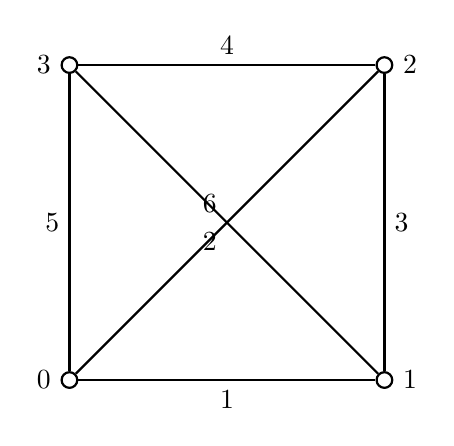
\begin{tikzpicture}
[nodedecorate/.style={shape=circle,inner sep=2pt,draw,thick},%
  linedecorate/.style={-,thick}]
% nodes or vertices
\node (0) at (0,0) [nodedecorate] {};
\node [left] at (0.west) {$0$};
\node (1) at (4,0) [nodedecorate] {};
\node [right] at (1.east) {$1$};
\node (2) at (4,4) [nodedecorate] {};
\node [right] at (2.east) {$2$};
\node (3) at (0,4) [nodedecorate] {};
\node [left] at (3.west) {$3$};
% edges or lines
\path
(0) edge[linedecorate] node[below]{$1$} (1)
(0) edge[linedecorate] node[below left] {$2$} (2)
(0) edge[linedecorate] node[left]{$5$} (3)
(1) edge[linedecorate] node[right]{$3$} (2)
(1) edge[linedecorate] node[above left] {$6$} (3)
(2) edge[linedecorate] node[above]{$4$} (3);
\end{tikzpicture}
}
\qquad
\subfigure[]{
\begin{tikzpicture}
[nodedecorate/.style={shape=circle,inner sep=2pt,draw,thick},%
  linedecorate/.style={-,thick}]
% nodes or vertices
\node (3) at (0,0) [nodedecorate] {};
\node [right] at (3.east) {$3$};
\node (2) at (1,2) [nodedecorate] {};
\node [right] at (2.east) {$2$};
\node (0) at (2,4) [nodedecorate] {};
\node [right] at (0.east) {$0$};
\node (1) at (3,6) [nodedecorate] {};
\node [right] at (1.east) {$1$};
% edges or lines
\path
(3) edge[linedecorate] node[left]{$4$} (2)
(2) edge[linedecorate] node[left]{$2$} (0)
(0) edge[linedecorate] node[left]{$1$} (1);
\end{tikzpicture}
}
\caption{An example of Borovka's algorithm. On the left is the
  original graph. On the right is the MST produced by Boruvka's algorithm.}
\label{fig:tree-forests:Boruvkas-algorithm}
\end{figure}

\end{example}



\begin{center}
\vskip .15in

\begin{Verbatim}[fontsize=\scriptsize,fontfamily=courier,fontshape=tt,frame=single,label=\sage]

def which_index(x,L):
    """
    L is a list of sublists (or tuple of sets or list
    of tuples, etc).

    Returns the index of the first sublist which x belongs
    to, or None if x is not in flatten(L).

    The 0-th element in
    Lx = [L.index(S) for S in L if x in S]
    almost works, but if the list is empty then Lx[0]
    throws an exception.

    EXAMPLES:
        sage: L = [[1,2,3],[4,5],[6,7,8]]
        sage: which_index(3,L)
        0
        sage: which_index(4,L)
        1
        sage: which_index(7,L)
        2
        sage: which_index(9,L)
        sage: which_index(9,L) == None
        True
    """
    for S in L:
        if x in S:
            return L.index(S)
    return None

def boruvka(G):
    """
    Implements Boruvka's algorithm to compute a MST of a graph.

    INPUT:
        G - a connected edge-weighted graph with distinct weights.
    OUTPUT:
        T - a minimum weight spanning tree.

    REFERENCES:
        http://en.wikipedia.org/wiki/Boruvka's_algorithm
    """
    T_vertices = [] # assumes G.vertices = range(n)
    T_edges = []
    T = Graph()
    E = G.edges() # a list of triples
    V = G.vertices()
    # start ugly hack to sort E
    Er = [list(x) for x in E]
    E0 = []
    for x in Er:
        x.reverse()
        E0.append(x)
    E0.sort()
    E = []
    for x in E0:
        x.reverse()
        E.append(tuple(x))
    # end ugly hack to get E is sorted by weight
    for e in E:
        # create about |V|/2 edges of T "cheaply"
        TV = T.vertices()
        if not(e[0] in TV) or not(e[1] in TV):
           T.add_edge(e)
    for e in E:
        # connect the "cheapest" components to get T
        C = T.connected_components_subgraphs()
        VC = [S.vertices() for S in C]
        if not(e in T.edges()) and (which_index(e[0],VC) != which_index(e[1],VC)):
           if T.is_connected():
                break
            T.add_edge(e)
    return T

\end{Verbatim}

\end{center}

Some examples using Sage:


\begin{center}
\fontsize{9pt}{9pt}
\selectfont
\tt
\begin{lstlisting}

        sage: A = matrix([[0,1,2,3],[4,0,5,6],[7,8,0,9],[10,11,12,0]])
        sage: G = DiGraph(A, format = "adjacency_matrix", weighted = True)
        sage: boruvka(G)
        Multi-graph on 4 vertices
        sage: boruvka(G).edges()
        [(0, 1, 1), (0, 2, 2), (0, 3, 3)]
        sage: A = matrix([[0,2,0,5,0,0,0],[0,0,8,9,7,0,0],[0,0,0,0,1,0,0],\
         [0,0,0,0,15,6,0],[0,0,0,0,0,3,4],[0,0,0,0,0,0,11],[0,0,0,0,0,0,0]])
        sage: G = Graph(A, format = "adjacency_matrix", weighted = True)
        sage: E = G.edges(); E
        [(0, 1, 2), (0, 3, 5), (1, 2, 8), (1, 3, 9), (1, 4, 7),
         (2, 4, 1), (3, 4, 15), (3, 5, 6), (4, 5, 3), (4,6, 4), (5, 6, 11)]
        sage: boruvka(G)
        Multi-graph on 7 vertices
        sage: boruvka(G).edges()
        [(0, 1, 2), (0, 3, 5), (2, 4, 1), (3, 5, 6), (4, 5, 3), (4, 6, 4)]
        sage: A = matrix([[0,1,2,5],[0,0,3,6],[0,0,0,4],[0,0,0,0]])
        sage: G = Graph(A, format = "adjacency_matrix", weighted = True)
        sage: boruvka(G).edges()
        [(0, 1, 1), (0, 2, 2), (2, 3, 4)]
        sage: A = matrix([[0,1,5,0,4],[0,0,0,0,3],[0,0,0,2,0],[0,0,0,0,0],[0,0,0,0,0]])
        sage: G = Graph(A, format = "adjacency_matrix", weighted = True)
        sage: boruvka(G).edges()
        [(0, 1, 1), (0, 2, 5), (1, 4, 3), (2, 3, 2)]

\end{lstlisting}
\end{center}
%

%%-----------------------------------------------------------------------%%
%%--- Binary trees ------------------------------------------------------%%

\section{Binary trees}

See section~3.3 of Gross and Yellen~\cite{GrossYellen1999}.

A binary tree is a rooted tree with at most 2 children per parent.

In this section, we consider

\begin{itemize}
\item binary codes,

\item Gray codes, and

\item Huffman codes.
\end{itemize}

\subsection{Binary codes}


\subsubsection{What is a code?}

A {\it code} is a rule for converting data in one
\index{code}
\index{codeword}
\index{alphabet}
format, or well-defined tangible representation,
into sequences of symbols in another format (and the finite set of symbols
used is called the {\it alphabet}). We shall identify a code
as a finite set of symbols which are the image
of the alphabet under this conversion rule. The elements of this set
are referred to as {\it codewords}. For example, using the ASCII code,
the letters in the English alphabet get converted into numbers
$\{0, 1, \dots, 255\}$. If these numbers are written in binary
then each codeword of a letter has length 8. In this way, we can
reformat, or encode, a ``string'' into a sequence of binary symbols (i.e.,
$0$'s and $1$'s).
{\it Encoding} is the conversion process one way.
{\it Decoding} is the reverse
\index{encode}
\index{decode}
process, converting these sequences of code-symbols back into information
in the original format.


Codes are used for

\begin{itemize}
\item
{\it Economy}. Sometimes this is called ``entropy encoding''
since there is an entropy function which describes how much information
a channel (with a given error rate) can carry and such
codes are designed to maximize entropy as best as possible.
In this case, in addition to simply being given an alphabet $A$, one
might be given a ``weighted alphabet,'' i.e., an alphabet for which each
symbol $a\in A$ is associated with a non-negative number
$w_a\geq 0$ (in practice, the probability that the
symbol $a$ occurs in a typical word).

\item
{\it Reliability}. Such codes are called ``error-correcting codes,''
since such codes are designed to communicate information
over a noisy channel in such a way that the errors in transmission are
likely to be correctable.

\item
{\it Security}. Such codes ae called ``cryptosystems.''
In this case, the inverse of the coding function $c:A\to B^*$ is designed to be
computationally infeasible. In other words, the coding function
$c$ is designed to be a ``trapdoor function.''

\end{itemize}

Other codes are merely simpler ways to communicate information
(flag semaphores, color codes, genetic codes, braille codes, musical scores, chess
notation, football diagrams, and so on), and have little or no
mathematical structure. We shall not study them.



\subsubsection{Basic definitions}

If every word in the code has the same length, the code is called
a {\it block code}. If a code is not a block code then it is called
a {\it variable-length} code.
\index{code!block}
\index{code!variable-length}
A {\it prefix-free} code is a code (typically one of variable-length)
with the property that there is no valid codeword in the code that
is a prefix (start) of any other codeword\footnote{In other words,
a codeword $s=s_1 \dots s_m$ is a {\it prefix} of a codeword
$t=t_1\dots t_n$ if and only if $m\leq n$ and
$s_1=t_1$, \dots, $s_m=t_m$. Codes which are prefix-free are easier
to decode than codes which are not prefix-free.}.
This is the {\it prefix-free condition}.
\index{code!prefix-free}

One example of a prefix-free code is the ASCII code.
Another example is

\[
00, 01, 100.
\]
On the other hand, a non-example is the code

\[
00, 01, 010, 100
\]
since the second codeword is a prefix of the third one.
Another non-example is Morse code recalled in
Table~\ref{tab:trees_forests:Morse_code} (we use $0$ for
$\cdot$ (``dit'') and $1$ for $-$ (``dah'')).
\index{code!Morse}

\begin{table}[!htbp]
\centering
\begin{tabular}{|c|c||c|c|} \hline
A & 01    & N & 10 \\
B & 1000  & O & 111 \\
C & 1010  & P & 0110 \\
D & 100   & Q & 1101 \\
E & 0     & R & 010 \\
F & 0010  & S & 000 \\
G & 110   & T & 1 \\
H & 0000  & U & 001 \\
I & 00    & V & 0001 \\
J & 0111  & W & 011 \\
K & 101   & X & 1001 \\
L & 0100  & Y & 1011 \\
M & 11    & Z & 1100 \\\hline
\end{tabular}
\caption{Morse code}
\label{tab:trees_forests:Morse_code}
\end{table}

For example, look at the Morse code for {\tt a} and the Morse code for
{\tt w}. These codewords violate the prefix-free condition.

\subsubsection{Gray codes}

History\footnote{This
history comes from an unpublished section 7.2.1.1
(``Generating all $n$-tuples'')
in volume 4 of Donald Knuth's {\bf The Art of Computer Programming}.
}
: Frank Gray (1887-1969) wrote about the so-called Gray codes in a
1951 paper published in the Bell System Technical Journal,
and then patented a device (used for television sets)
based on it in 1953. However, the idea of a binary Gray code
appeared earlier. In fact, it appeared in an earlier patent
(one by Stibitz in 1943). It was also used in E. Baudot's
(a French engineer) telegraph machine of 1878 and in
a French booklet by L. Gros on the solution to the
``Chinese ring puzzle'' published in 1872.

The term ``Gray code'' is ambiguous. It is actually a
large family of sequences of $n$-tuples. Let
${\mathbb{Z}}_m=\{0,1,\dots,m-1\}$. More precisely, an
{\it $m$-ary Gray code of length $n$} (called a {\it binary
Gray code} when $m=2$) is a sequence of
all possible (namely, $N=m^n$) $n$-tuples
\index{Gray code!binary}
\index{Gray code!$m$-ary}

\[
g_1,g_2,\dots, g_N,
\]
where
\begin{itemize}
\item
each $g_i\in {\mathbb{Z}}_m^n$,
\item
$g_i$ and $g_{i+1}$ differ by $1$ in exactly one
coordinate.
\end{itemize}
In other words, an $m$-ary Gray code of length
$n$ is a particular way to order the set of all
$m^n$ $n$-tuples whose coordinates are taken from
${\mathbb{Z}}_m$. From the transmission/communication
perspective, this sequence has two advantages:

\begin{itemize}
\item
It is easy and fast to produce the sequence, since
successive entries differ in only one coordinate.

\item
An error is relatively easy to detect, since you can
compare an $n$-tuple with the previous one. If they
difer in more than one coordinate, you know an error
was made.

\end{itemize}

\begin{example}
{\rm
Here is a $3$-ary Gray code of length $2$:

\[
[0, 0], [1, 0], [2, 0], [2, 1], [1, 1], [0, 1], [0, 2], [1, 2], [2, 2]
\]
and here is a binary Gray code of length $3$:

\[
[0, 0, 0], [1, 0, 0], [1, 1, 0], [0, 1, 0], [0, 1, 1], [1, 1, 1], [1, 0, 1], [0, 0, 1].
\]
}
\end{example}

Gray codes have applications to engineering,
recreational mathematics (solving the Tower of Hanoi
puzzle, ``The Brain'' puzzle, the ``Chinese ring puzzle'',
and others), and to mathematics (for example, aspects of
combinatorics, computational group theory
and the computational aspects of linear codes).

\subsubsection{Binary Gray codes}

Consider the so-called $n$-hypercube graph
$Q_n$. This can be envisioned as the graph whose
vertices are the vertices of a cube in
$n$-space
\index{graph!hypercube}

\[
\{(x_1,\dots,x_n)\ |\ 0\leq x_i\leq 1\},
\]
and whose edges are those line segments in
${\mathbb{R}}^n$ connecting two ``neighboring''
vertices (namely, two vertices which differ
in exactly one coordinate).
A binary Gray code of length $n$ can be regarded as a
path on the hypercube graph $Q_n$ which visits
each vertex of the cube exactly once.
In other words, a binary Gray code of length $n$
may be identified with a
Hamiltonian cycle on the graph $Q_n$
(see Figure \ref{fig:trees_forests:gray_code_cube} for an example).

\begin{figure}[!htbp]
\centering
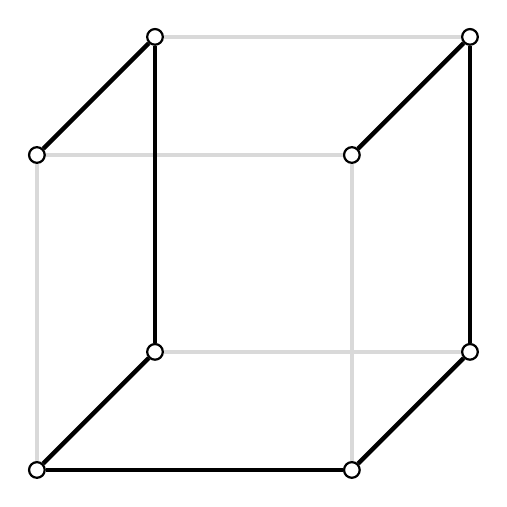
\begin{tikzpicture}
[nodedecorate/.style={shape=circle,inner sep=2pt,draw,thick},%
  darkline/.style={-,ultra thick},
  lightline/.style={-,ultra thick,color=gray!30}]
% nodes or vertices
% foreground square
\node (1) at (0,0) [nodedecorate] {};
\node (2) at (4,0) [nodedecorate] {};
\node (3) at (4,4) [nodedecorate] {};
\node (4) at (0,4) [nodedecorate] {};
% background square
\node (5) at (1.5,1.5) [nodedecorate] {};
\node (6) at (5.5,1.5) [nodedecorate] {};
\node (7) at (5.5,5.5) [nodedecorate] {};
\node (8) at (1.5,5.5) [nodedecorate] {};
% edges or lines
\path
% foreground square
(1) edge[darkline] node {} (2)
(2) edge[lightline] node {} (3)
(3) edge[lightline] node {} (4)
(4) edge[lightline] node {} (1)
% background square
(5) edge[lightline] node {} (6)
(6) edge[darkline] node {} (7)
(7) edge[lightline] node {} (8)
(8) edge[darkline] node {} (5)
% joining foreground and background squares
(1) edge[darkline] node {} (5)
(2) edge[darkline] node {} (6)
(3) edge[darkline] node {} (7)
(4) edge[darkline] node {} (8);
\end{tikzpicture}
\caption{Viewing $\Gamma_3$ as a Hamiltonian path on $Q_3$.}
\label{fig:trees_forests:gray_code_cube}
\end{figure}


How do you efficiently compute a Gray code?

Perhaps the simplest way to state the idea of
quickly constructing
the {\it reflected binary Gray code} $\Gamma_n$
of length $n$ is as follows:

\[
\Gamma_0=[],\ \ \ \
\Gamma_{n}=[0,\Gamma_{n-1}],[1,\Gamma_{n-1}^{rev}],
\]
where $\Gamma_m^{rev}$ means the Gray code in
reverse order. For instance, we have

\[
\Gamma_0=[],
\]
\[
\Gamma_1 = [0], [1],
\]
\[
\Gamma_2=[[0,0],[0,1],[1,1],[1,0],
\]
and so on. This is a nice procedure if you want to create
the entire list at once (which, by the way, gets very long
very fast).

An implementation of the reflected Gray code using Python is given below.

\begin{Verbatim}[fontsize=\scriptsize,fontfamily=courier,fontshape=tt,frame=single,label=Python
  3.0]

def graycode(length,modulus):
    """
    Returns the n-tuple reflected Gray code mod m.


    EXAMPLES:
        sage: graycode(2,4)

        [[0, 0],
         [1, 0],
         [2, 0],
         [3, 0],
         [3, 1],
         [2, 1],
         [1, 1],
         [0, 1],
         [0, 2],
         [1, 2],
         [2, 2],
         [3, 2],
         [3, 3],
         [2, 3],
         [1, 3],
         [0, 3]]

    """
    n,m = length,modulus
    F = range(m)
    if n == 1:
        return [[i] for i in F]
    L = graycode(n-1, m)
    M = []
    for j in F:
        M = M+[ll+[j] for ll in L]
    k = len(M)
    Mr = [0]*m
    for i in range(m-1):
        i1 = i*int(k/m)       # this requires Python 3.0 or Sage
        i2 = (i+1)*int(k/m)
        Mr[i] = M[i1:i2]
    Mr[m-1] = M[(m-1)*int(k/m):]
    for i in range(m):
        if is_odd(i):
            Mr[i].reverse()
    M0 = []
    for i in range(m):
        M0 = M0+Mr[i]
    return M0

\end{Verbatim}

\vskip .2in
Consider the reflected binary code
of length $8$, $\Gamma_8$. This has $2^8=256$ codewords.
\sage can easily create the list plot of the coordinates
$(x,y)$, where $x$ is an integer $j \in {\mathbb{Z}}_{256}$
which indexes the codewords in $\Gamma_8$
and the corresponding $y$ is the $j$-th
codeword in $\Gamma_8$ converted to decimal.
This will give us some idea of how the Gray code
``looks'' in some sense. The plot is given in Figure \ref{fig:Gamma8}.

%% Figure created using the following code.
%% def int2binary(m, n):
%%    '''
%%    returns GF(2) vector of length n obtained
%%    from the binary repr of m, padded by 0's
%%    (on the left) to length n.
%%
%%    EXAMPLES:
%%        sage: for j in range(8):
%%        ....:     print int2binary(j,3)+int2binary(int(j/2),3)
%%        ....:
%%        (0, 0, 0)
%%        (0, 0, 1)
%%        (0, 1, 1)
%%        (0, 1, 0)
%%        (1, 1, 0)
%%        (1, 1, 1)
%%        (1, 0, 1)
%%        (1, 0, 0)
%%    '''
%%    s = bin(m)
%%    k = len(s)
%%    F = GF(2)
%%    b = [F(0)]*n
%%    for i in range(2,k):
%%        b[n-k+i] = F(int(s[i]))
%%    return vector(b)
%%
%% def binary2int(b):
%%    "''
%%    inverts int2binary
%%
%%    "''
%%    k = len(b)
%%    n = sum([int(b[i])*2**(k-1-i) for i in range(k)])
%%    return n
%%
%% def graycodeword(m, n):
%%    '''
%%    returns the mth codeword in the reflected binary Gray code
%%    of length n.
%%
%%    EXAMPLES:
%%        sage: graycodeword(3,3)
%%        (0, 1, 0)
%%    '''
%%    return int2binary(m,n)+int2binary(int(m/2),n)
%%
%% sage: L = [(k,binary2int(graycodeword(k, 8))) for k in range(256)]
%% sage: P = list_plot(L); P.save(``gray-code-2-8.png'')
\begin{figure}[!htbp]
\centering
\includegraphics{image/graycode-gamma8}
\caption{List plot of $\Gamma_8$ created using Sage.}
\label{}
\end{figure}

What if you only want to compute the
$i$-th Gray codeword in the Gray code of length $n$?
Can it be computed quickly as well without computing the
entire list?
At least in the case of the reflected binary Gray code, there
is a very simple way to do this. The $k$-th element in the
above-described reflected binary Gray code of length $n$
is obtained by simply adding the binary representation of
$k$ to the binary representation of the integer part of
$k/2$.

An example using \sage is given below.

\begin{Verbatim}[fontsize=\scriptsize,fontfamily=courier,fontshape=tt,frame=single,label=\sage]

def int2binary(m, n):
    '''
    returns GF(2) vector of length n obtained
    from the binary repr of m, padded by 0's
    (on the left) to length n.

    EXAMPLES:
        sage: for j in range(8):
        ....:     print int2binary(j,3)+int2binary(int(j/2),3)
        ....:
        (0, 0, 0)
        (0, 0, 1)
        (0, 1, 1)
        (0, 1, 0)
        (1, 1, 0)
        (1, 1, 1)
        (1, 0, 1)
        (1, 0, 0)
    '''
    s = bin(m)
    k = len(s)
    F = GF(2)
    b = [F(0)]*n
    for i in range(2,k):
        b[n-k+i] = F(int(s[i]))
    return vector(b)

def graycodeword(m, n):
    '''
    returns the kth codeword in the reflected binary Gray code
    of length n.

    EXAMPLES:
        sage: graycodeword(3,3)
        (0, 1, 0)
    '''
    return int2binary(m,n)+int2binary(int(m/2),n)

\end{Verbatim}

\begin{exercise}
Convert the above function {\tt graycodeword} into a pure Python
function.
\end{exercise}


%%-----------------------------------------------------------------------%%
%%--- Huffman codes -----------------------------------------------------%%

\section{Huffman codes}
\label{sec:trees_forests:Huffman_codes}

An \emph{alphabet}\index{alphabet} $A$ is a finite set whose elements
are referred to as \emph{symbols}. A \emph{word}\index{word} (or
\emph{string}\index{string} or \emph{message}\index{message}) over $A$
is a finite sequence of symbols in $A$ and the \emph{length} of the
word is the number of symbols it contains. A word is usually written
by concatenating symbols together: $a_1 a_2 \cdots a_k$ ($a_i \in A$)
is a word of length $k$.

A commonly occurring alphabet in practice is the \emph{binary alphabet}
$\{0,1\}$. A word over the binary alphabet is a finite sequence of
$0$'s and $1$'s. If $A$ is an alphabet, let $A^*$ denote the set of
all words in $A$. The length of a word is denoted by vertical
bars. That is, if $w = a_1 \cdots a_k$ is a word over $A$, then define
$|w|: A^* \longrightarrow \ZZ$ by
\[
|w|
=
|a_1 \cdots a_k|
=
k.
\]
Let $A$ and $B$ be two alphabets. A \emph{code}\index{code} for $A$
using $B$ is an injection $c: A \longrightarrow B^*$. By abuse of
notation, we often denote the code simply by the set
\[
C
=
c(A)
=
\{c(a) \;|\; a \in A\}.
\]
The elements of $C$ are called \emph{codewords}\index{codeword}. If
$B$ is the binary alphabet, then $C$ is called a
\emph{binary code}\index{code!binary}.


%%--- Tree representation -----------------------------------------------%%

\subsection{Tree representation}

Any binary code can be represented by a tree, as
Example~\ref{eg:tree_forests:binary_code_tree_representation} shows.

\begin{example}
\label{eg:tree_forests:binary_code_tree_representation}
Let $\BB_\ell$ be the binary code of length $\leq \ell$. Represent
codewords of $\BB_\ell$ using trees.
\end{example}

\begin{proof}[Solution]
Here is how to represent the code $\BB_\ell$ consisting of all binary
strings of length $\leq \ell$. Start with the
\emph{root node}\index{node!root} $\varepsilon$\index{$\varepsilon$}
being the empty string. The two children of this node, $v_0$ and
$v_1$, correspond to the two strings of length $1$. Label $v_0$ with a
``$0$'' and $v_1$ with a ``$1$''. The two children of $v_0$,
i.e. $v_{00}$ and $v_{01}$, correspond to the strings of length $2$
which start with a $0$. Similarly, the  two children of $v_1$,
i.e. $v_{10}$ and $v_{11}$, correspond to the strings of length $2$
that each starts with a $1$. Continue creating child nodes until we
reach length $\ell$, at which point we stop. There are a total of
$2^{\ell + 1} - 1$ nodes in this tree and $2^\ell$ of them are
\emph{leaves}\index{leaf}~(vertices of a tree with degree $1$,
i.e. childless nodes). Note that the parent of any node is a prefix to
that node. Label each node $v_s$ with the string ``$s$'', where $s$ is
a binary sequence of length $\leq \ell$. See
Figure~\ref{fig:trees_forests:tree_representation_B_2} for an example
when $\ell = 2$.
\end{proof}

\begin{figure}[!htbp]
\centering
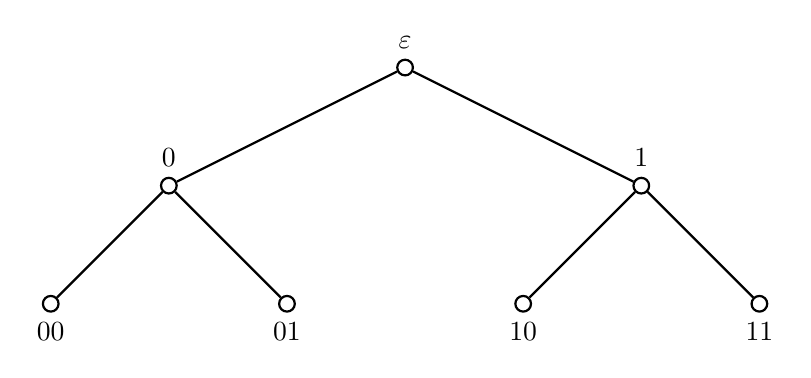
\begin{tikzpicture}
[nodedecorate/.style={shape=circle,inner sep=2pt,draw,thick},%
  linedecorate/.style={-,thick},%
  scale=1.5]
%% nodes or vertices
\foreach \nodename/\x/\y/\direction/\navigate in {
  00/0/0/below/south, 01/2/0/below/south, 10/4/0/below/south,
  11/6/0/below/south, 0/1/1/above/north, 1/5/1/above/north} {
  \node (\nodename) at (\x,\y) [nodedecorate] {};
  \node [\direction] at (\nodename.\navigate) {$\nodename$};
}
\node (e) at (3,2) [nodedecorate] {};
\node [above] at (e.north) {$\varepsilon$};
%% edges or lines
\path
\foreach \startnode/\endnode in {0/00, 0/01, 1/10, 1/11, e/0, e/1} {
  (\startnode) edge[linedecorate] node {} (\endnode)
};
\end{tikzpicture}
\caption{Tree representation of the binary code $\BB_2$.}
\label{fig:trees_forests:tree_representation_B_2}
\end{figure}

In general, if $C$ is a code contained in $\BB_\ell$, then to create
the tree for $C$, start with the tree for $\BB_\ell$. First, remove
all nodes associated to a binary string for which it and all of its
descendents are not in $C$. Next, remove all labels which do not
correspond to codewords in $C$. The resulting labeled graph is the
tree associated to the binary code $C$.
\index{code!tree}

For visualizing the construction of Huffman codes later, it is
important to see that one can \emph{reverse} this construction to
start from such a binary tree and recover a binary code from it. The
codewords are determined by the following rules:
%
\begin{itemize}
\item The root node gets the empty codeword.

\item Each left-ward branch gets a $0$ appended to the end of its
  parent. Each right-ward branch gets a $1$ appended to the end.
\end{itemize}


%%--- Uniquely decodable codes ------------------------------------------%%

\subsection{Uniquely decodable codes}

If $c: A \longrightarrow B^*$ is a code, then we can extend $c$ to
$A^*$ by \emph{concatenation}:
\[
c(a_1 a_2 \cdots a_k)
=
c(a_1) c(a_2) \cdots c(a_k).
\]
If the extension $c: A^* \longrightarrow T^*$ is also an injection,
then $c$ is called \emph{uniquely decodable}.
\index{code!uniquely decodable}

\begin{example}
Is the Morse code\index{code!Morse} in
Table~\ref{tab:trees_forests:Morse_code} uniquely decodable? Why or
why not?
\end{example}

\begin{proof}[Solution]
Note that these Morse codewords all have lengths less than or equal to
$4$. Other commonly occurring symbols used~(the digits $0$ through
$9$, punctuation symbols, and some others) are also encodable in Morse
code, but they use longer codewords.

Let $A$ denote the English alphabet, $B = \{0, 1\}$ the binary
alphabet, and $C: A \longrightarrow B^*$ the Morse code. Since
$c(ET) = 01 = c(A)$, it is clear that the Morse code is \emph{not}
uniquely decodable.
\end{proof}

In fact, prefix-free implies uniquely decodable.

\begin{theorem}
If a code $c: A \longrightarrow B^*$ is prefix-free, then it is
uniquely decodable.
\end{theorem}

\begin{proof}
We use induction on the length of a message. We want to show that if
$x_1 \cdots x_k$ and $y_1 \cdots y_\ell$ are messages with
$c(x_1) \cdots c(x_k) = c(y_1) \cdots c(y_\ell)$, then
$x_1 \cdots x_k = y_1 \cdots y_\ell$. This in turn implies $k = \ell$
and $x_i = y_i$ for all $i$.

The case of length $1$ follows from the fact that
$c: A \longrightarrow B^*$ is injective~(by the definition of a
code).

Suppose that the statement of the theorem holds for all
codes of length $< m$. We must show that the length $m$ case is
true. Suppose $c(x_1) \cdots c(x_k) = c(y_1) \cdots c(y_\ell)$, where
$m = \max(k, \ell)$. These strings are equal, so the substring
$c(x_1)$ of the left-hand side and the substring $c(y_1)$ of the
right-hand side are either equal or one is contained in the other. If,
say, $c(x_1)$ is properly contained in $c(y_1)$, then $c$ is not
prefix-free. Likewise if $c(y_1)$ is properly contained in
$c(x_1)$. Therefore, $c(x_1) = c(y_1)$, which implies $x_1 = y_1$. Now
remove this codeword from both sides, so
$c(x_2) \cdots c(x_k) = c(y_2) \cdots c(y_\ell)$. By the induction
hypothesis, $x_2 \cdots x_k = y_2 \cdots y_\ell$. These facts together
imply $k = \ell$ and $x_i = y_i$ for all $i$.
\end{proof}

Consider now a weighted alphabet $(A,p)$, where
$p: A \longrightarrow [0,1]$ satisfies $\sum_{a \in A}p(a) = 1$, and a
code $c: A \longrightarrow B^*$. In other words, $p$ is a probability
distribution on $A$. Think of $p(a)$ as the probability that the
symbol $a$ arises in an typical message. The
\emph{average word length} $L(c)$ is\footnote{
  In probability terminology, this is the expected value $E(X)$ of the
  random variable $X$ which assigns to a randomly selected symbol in
  $A$, the length of the associated codeword in $C$.
}
\[
L(c)
=
\sum_{a \in A} p(a) \cdot |c(a)|
\]
where $|\cdot|$ denotes the \emph{length} of a codeword.
\index{length of codeword}
Given a weighted alphabet $(A,p)$ as above, a code
$c: A \longrightarrow B^*$ is called \emph{optimal} if there is no
such code with a smaller average word length.
\index{code!optimal}
Optimal codes satisfy the following amazing property. For a proof,
which is very easy and highly recommended for anyone who is curious to
see more, refer to section~3.6 of Biggs~\cite{Biggs2009}.

\begin{lemma}
\label{lem:trees_forests:binary_optimal_prefix_free_code}
Suppose $c: A \longrightarrow B^*$ is a binary optimal prefix-free
code and let $\ell = \max_{a \in A} \big(|c(a)|\big)$ denote the
maximum length of a codeword. The following statements hold.
%
\begin{enumerate}
\item If $|c(a')|>|c(a)|$, then $p(a')\leq p(a)$.

\item The subset of codewords of length $\ell$,
\[
C_\ell
=
\{c \in c(A) \;|\; \ell = |c(a)|\},
\]
contains two codewords of the form $b0$ and $b1$ for some $b \in B^*$.
\end{enumerate}
\end{lemma}


%%--- Huffman coding ----------------------------------------------------%%

\subsection{Huffman coding}

The Huffman code construction is based on the second property in
Lemma~\ref{lem:trees_forests:binary_optimal_prefix_free_code}. Using
this property, in 1952 David Huffman~\cite{Huffman1952} presented an
optimal prefix-free binary code, which has since been named Huffman
code.

Here is the recursive/inductive construction of a Huffman code. We
shall regard the binary Huffman code as a tree, as described
above. Suppose that the weighted alphabet $(A,p)$ has $n$ symbols. We
assume inductively that there is an optimal prefix-free binary code
for any weighted alphabet $(A',p')$ having $<n$ symbols.

\begin{description}
\item[Huffman's rule 1] Let $a,a' \in A$ be symbols with the smallest
  weights. Construct a new weighted alphabet with $a,a'$ replaced by
  the single symbol $a^* = aa'$ and having weight
  $p(a^*) = p(a) + p(a')$. All other symbols and weights remain
  unchanged.

\item[Huffman's rule 2] For the code $(A',p')$ above, if $a^*$ is
  encoded as the binary string $s$, then the encoded binary string for
  $a$ is $s0$ and the encoded binary string for $a'$ is $s1$.
\end{description}

The above two rules tell us how to inductively build the tree
representation for the Huffman code of $(A,p)$ up from its
leaves~(associated to the low weight symbols).
%
\begin{itemize}
\item Find two different symbols of lowest weight, $a$ and $a'$. If
  two such symbols do not exist, stop. Replace the weighted alphabet
  with the new weighted alphabet as in Huffman's rule 1.

\item Add two nodes~(labeled with $a$ and $a'$, respectively) to the
  tree, with parent $a^*$ (see Huffman's rule 1).

\item If there are no remaining symbols in $A$, label the parent $a^*$
  with the empty set and stop. Otherwise, go to the first step.
\end{itemize}

These ideas are captured in
Algorithm~\ref{alg:trees_forests:binary_tree_Huffman_codes}, which
outlines steps to construct a binary tree corresponding to the Huffman
code of an alphabet.
Line~\ref{alg:Huffman_tree:initialize_priority_queue} initializes a
minimum priority queue $Q$ with the symbols in the alphabet $A$.
Line~\ref{alg:Huffman_tree:empty_binary_tree} creates an empty binary
tree that will be used to represent the Huffman code corresponding to
$A$. The for loop from lines~\ref{alg:Huffman_tree:for_loop:start}
to~\ref{alg:Huffman_tree:insert_into_queue} repeatedly extracts from
$Q$ two elements $a$ and $b$ of minimum weights. We then create a new
vertex $z$ for the tree $T$ and also let $a$ and $b$ be vertices of
$T$. The weight $W[z]$ of $z$ is the sum of the weights of $a$ and
$b$. We let $z$ be the parent of $a$ and $b$, and insert the new edges
$za$ and $zb$ into $T$. The newly created vertex $z$ is now inserted
into $Q$ with priority $W[z]$. After $n - 1$ rounds of the for loop,
the priority queue has only one element in it, namely the root $r$ of
the binary tree $T$. We extract $r$ from
$Q$~(line~\ref{alg:Huffman_tree:extract_tree_root}) and return it
together with $T$~(line~\ref{alg:Huffman_tree:return_tree_and_root}).

\begin{algorithm}[!htpb]
\dontprintsemicolon  % no semicolon at end of pseudocode statements
%% data section
\SetKwInOut{Input}{Input}
\SetKwInOut{Output}{Output}
%% input/output
\Input{An alphabet $A$ of $n$ symbols. A weight list $W$ of size $n$
  such that $W[i]$ is the weight of $a_i \in A$.}
\Output{A binary tree $T$ representing the Huffman code of $A$ and the
  root $r$ of $T$.}
\BlankLine
%% algorithm body
$n \leftarrow |A|$\;
$Q \leftarrow A$~\nllabel{alg:Huffman_tree:initialize_priority_queue}~\tcc*[f]{minimum priority queue}\;
$T \leftarrow \text{empty tree}$~\nllabel{alg:Huffman_tree:empty_binary_tree}\;
\For{$i \leftarrow 1, 2, \dots, n-1$~\nllabel{alg:Huffman_tree:for_loop:start}}{
  $a \leftarrow \extractMin(Q)$\;
  $b \leftarrow \extractMin(Q)$\;
  $z \leftarrow$ node with left child $a$ and right child $b$\;
  add the edges $za$ and $zb$ to $T$\;
  $W[z] \leftarrow W[a] + W[b]$\;
  insert $z$ into priority queue $Q$~\nllabel{alg:Huffman_tree:insert_into_queue}\;
}
$r \leftarrow \extractMin(Q)$~\nllabel{alg:Huffman_tree:extract_tree_root}\;
\Return $(T, r)$~\nllabel{alg:Huffman_tree:return_tree_and_root}\;
\caption{Binary tree representation of Huffman codes.}
\label{alg:trees_forests:binary_tree_Huffman_codes}
\end{algorithm}

The running time analysis of
Algorithm~\ref{alg:trees_forests:binary_tree_Huffman_codes} depends on
the implementation of the priority queue $Q$. Suppose $Q$ is a simple
unsorted list. The initialization on
line~\ref{alg:Huffman_tree:initialize_priority_queue} requires $O(n)$
time. The for loop from line~\ref{alg:Huffman_tree:for_loop:start}
to~\ref{alg:Huffman_tree:insert_into_queue} is executed exactly
$n - 1$ times. Searching $Q$ to determine the element of minimum
weight requires time at most $O(n)$. Determining two elements of
minimum weights requires time $O(2n)$. The for loop requires time
$O(2n^2)$, which is also the time requirement for the algorithm. An
efficient implementation of the priority queue $Q$, e.g. as a binary
minimum heap, can lower the running time of
Algorithm~\ref{alg:trees_forests:binary_tree_Huffman_codes} down to
$O(n \log_2(n))$.

Algorithm~\ref{alg:trees_forests:binary_tree_Huffman_codes} represents
the Huffman code of an alphabet as a binary tree $T$ rooted at $r$. To
determine the actual encoding of each symbol in the alphabet, we feed
$T$ and $r$ to
Algorithm~\ref{alg:trees_forests:Huffman_encoding_alphabet} to obtain
the encoding of each symbol. Starting from the root $r$ whose
designated label is the empty string $\varepsilon$, the algorithm
traverses the vertices of $T$ in a breadth-first search fashion. If
$v$ is an internal vertex with label \verb!e!, the label of its left
child is the concatenation \verb!e0! and for the rigth child of $v$ we
assign the label \verb!e1!. If $v$ happens to be a leaf vertex, we
take its label to be its Huffman encoding. Any Huffman encoding
assigned to a symbol of an alphabet is not unique. Either of the two
children of an internal vertex can be designated as the left
(resp. right) vertex. The running time of
Algorithm~\ref{alg:trees_forests:Huffman_encoding_alphabet} is
$O(|V|)$, where $V$ is the vertex set of $T$.

\begin{algorithm}[!htpb]
\dontprintsemicolon  % no semicolon at end of pseudocode statements
%% data section
\SetKwInOut{Input}{Input}
\SetKwInOut{Output}{Output}
\SetKwData{treeRoot}{root}
\SetKwData{one}{1}
\SetKwData{zero}{0}
%% input/output
\Input{A binary tree $T$ representing the Huffman code of an alphabet
  $A$. The root $r$ of $T$.}
\Output{A list $H$ representing a Huffman code of $A$, where $H[a_i]$
  corresponds to a Huffman encoding of $a_i \in A$.}
\BlankLine
%% algorithm body
$H \leftarrow [\,]$~\tcc*[f]{list of Huffman encodings}\;
$Q \leftarrow [r]$~\tcc*[f]{queue of vertices}\;
\While{$\length(Q) > 0$}{
  $\treeRoot \leftarrow \dequeue(Q)$\;
  \eIf{\treeRoot \emph{is a leaf}}{
    $H[\treeRoot] \leftarrow$ label of \treeRoot\;
  }{
    $a \leftarrow$ left child of \treeRoot\;
    $b \leftarrow$ right child of \treeRoot\;
    $\enqueue(Q, a)$\;
    $\enqueue(Q, b)$\;
    label of $a \leftarrow$ label of \treeRoot $+$ \zero\;
    label of $b \leftarrow$ label of \treeRoot $+$ \one\;
  }
}
\Return $H$\;
\caption{Huffman encoding of an alphabet.}
\label{alg:trees_forests:Huffman_encoding_alphabet}
\end{algorithm}

\begin{example}
Consider the alphabet $A = \{a, b, c, d, e, f\}$ with corresponding
weights $w(a) = 19$, $w(b) = 2$, $w(c) = 40$, $w(d) = 25$,
$w(e) = 31$, and $w(f) = 3$. Construct a binary tree representation of
the Huffman code of $A$ and determine the encoding of each symbol of
$A$.
\end{example}

\begin{proof}[Solution]
Use Algorithm~\ref{alg:trees_forests:binary_tree_Huffman_codes} to
construct a binary tree representation of the weighted alphabet
$A$. The resulting binary tree $T$ is shown in
Figure~\ref{fig:trees_forests:eg:binary_tree_Huffman_encodings:binary_tree},
where $a_i: w_i$ is an abbreviation for ``vertex $a_i$ has weight
$w_i$.'' The binary tree is rooted at $k$. To encode each alphabetic
symbol, input $T$ and $k$ into
Algorithm~\ref{alg:trees_forests:Huffman_encoding_alphabet} to get the
encodings shown in
Figure~\ref{fig:trees_forests:eg:binary_tree_Huffman_encodings:Huffman_encodings}.
\end{proof}

\begin{figure}[!htbp]
\centering
\subfigure[]{
\label{fig:trees_forests:eg:binary_tree_Huffman_encodings:binary_tree}
\begin{tikzpicture}
[linedecorate/.style={-,thick},%
  scale=1.5]
%% nodes or vertices
\foreach \nodename/\weight/\x/\y in {b/2/0/0, f/3/1/0, g/5/0.5/1,
  a/19/1.5/1, h/24/1/2, d/25/2/2, e/31/3/2, c/40/4/2, i/49/1.5/3,
  j/71/3.5/3, k/120/2.5/4} {
  \node (\nodename) at (\x,\y) [] {$\nodename:\weight$};
}
%% \node (e) at (3,2) [nodedecorate] {};
%% \node [above] at (e.north) {$\varepsilon$};
%% %% edges or lines
\path
\foreach \startnode/\endnode in {g/b, g/f, h/g, h/a, i/h, i/d, j/e,
  j/c, k/i, k/j} {
  (\startnode) edge[linedecorate] node {} (\endnode)
};
\end{tikzpicture}
}
%%
%%
\subfigure[]{
\label{fig:trees_forests:eg:binary_tree_Huffman_encodings:Huffman_encodings}
\begin{tikzpicture}
[linedecorate/.style={-,thick},%
  scale=1.5]
%% nodes or vertices
\foreach \nodename/\code/\x/\y in {b/0000/0/0, f/0001/1/0, g/000/0.5/1,
  a/001/1.5/1, h/00/1/2, d/01/2/2, e/10/3/2, c/11/4/2, i/0/1.5/3,
  j/1/3.5/3, k/$\varepsilon$/2.5/4} {
  \node (\nodename) at (\x,\y) [] {$\texttt{\code}$};
}
%% \node (e) at (3,2) [nodedecorate] {};
%% \node [above] at (e.north) {$\varepsilon$};
%% %% edges or lines
\path
\foreach \startnode/\endnode in {g/b, g/f, h/g, h/a, i/h, i/d, j/e,
  j/c, k/i, k/j} {
  (\startnode) edge[linedecorate] node {} (\endnode)
};
\end{tikzpicture}
}
\caption{Binary tree representation of an alphabet and its Huffman encodings.}
\label{fig:trees_forests:eg:binary_tree_Huffman_encodings}
\end{figure}


%%-----------------------------------------------------------------------%%
%%--- Problems ----------------------------------------------------------%%

\subsection*{Problems~\ref{sec:trees_forests:Huffman_codes}}

\begin{enumerate}
\item Show by giving an example that the Morse code is not
  prefix-free.

\item Consider the alphabet $A = \{a,b,c\}$ with corresponding
  probabilities~(or weights) $p(a) = 0.5$, $p(b) = 0.3$, and
  $p(c) = 0.2$. Generate two different Huffman codes for $A$ and
  illustrate the tree representations of those codes.

\item Find the Huffman code for the letters of the English alphabet
  weighted by the frequency of common American usage.\footnote{
    You can find this on the Internet or in the literature. Part of
    this exercise is finding this frequency distribution yourself.}
\end{enumerate}


%%%%%%%%%%%%%%%%%%%%%%%%%%%%%%%%%%%%%%%%%%

\section{Applications to computer science}


%%-----------------------------------------------------------------------%%
%%--- Tree traversals ---------------------------------------------------%%

\subsection{Tree traversals}

See section~3.5 of Gross and Yellen~\cite{GrossYellen1999}.
See also \url{http://en.wikipedia.org/wiki/Tree_traversal}.

\begin{itemize}
\item stacks and queues

\item breadth-first, or level-order, traversal

\item depth-first, or pre-order, traversal

\item post-order traversal

\item symmetric, or in-order, traversal
\end{itemize}

In computer science, {\it tree traversal} refers to the process of
examining each node in a tree data structure exactly once.
\index{tree traversal}
We restrict our discussion to binary rooted trees.

Starting at the root of a binary tree, there are three main steps that
can be performed and the order in which they are performed defines the
traversal type.

\noindent
{\it Depth-first traversal}:
\index{tree traversal!depth-first}
\index{tree traversal!pre-order}
\begin{itemize}
\item
Visit the root vertex.

\item
Traverse the left subtree recursively.

\item
Traverse the right subtree recursively.

\end{itemize}


\noindent
{\it Breadth-first traversal}:
\index{tree traversal!breadth-first}
\index{tree traversal!level-order}
\begin{itemize}
\item
Initialize $i=0$ and set $N$ equal to the maximum depth
of the tree (i.e., the maximum distance from the root vertex
to any other vertex in the tree).
\index{tree!depth}

\item
Visit the vertices of depth $i$.

\item
Increment $i=i+1$. If $i>N$ then stop. Otherwise, go to
the previous step.

\end{itemize}


\noindent
{\it post-order traversal}:
\index{tree traversal!post-order}
\begin{itemize}
\item
Traverse the left subtree recursively.

\item
Visit the root vertex.

\item
Traverse the right subtree recursively.

\end{itemize}


\noindent
{\it symmetric traversal}:
\index{tree traversal!symmetric}
\index{tree traversal!in-order}
\begin{itemize}
\item
Traverse the left subtree recursively.

\item
Visit the root vertex.

\item
Traverse the right subtree recursively.

\end{itemize}

%%-----------------------------------------------------------------------%%
%%--- Binary search trees -----------------------------------------------%%

\subsection{Binary search trees}

See section~3.6 of Gross and Yellen~\cite{GrossYellen1999}, and
chapter~12 of Cormen~et~al.~\cite{CormenEtAl2001}. See also
\url{http://en.wikipedia.org/wiki/Binary_search_tree}.


\begin{itemize}
\item records and keys

\item searching a binary search tree (BST)

\item inserting into a BST

\item deleting from a BST

\item traversing a BST

\item sorting using BST
\end{itemize}

A {\it binary search tree} (BST) is a rooted binary tree
$T=(V,E)$ having weighted vertices ${\rm wt}:V\to {\mathbb{R}}$ satisfying:
\index{binary search tree}
\index{BST}

\begin{itemize}
\item
 The left subtree of a vertex $v$ contains only vertices whose label
(or ``key'') is less than the label of $v$.
\item
The right subtree of a vertex $v$ contains only vertices whose label
  is greater than the label of $v$.
\item
Both the left and right subtrees must also be binary search trees.
\end{itemize}

From the above properties it naturally follows that:
{\it Each vertex has a distinct label.}


\subsubsection{Traversal}

The vertices of a BST $T$ can be visited retrieved in-order of the
weights of the vertices (i.e.,
using a symmetric search type) by recursively  traversing the left subtree of the
root vertex, then accessing the root vertex itself, then recursively traversing the
right subtree of the root node.

\subsubsection{Searching}

We are given a BST (i.e., a binary rooted tree with weighted vertices
having distinct weights satisfying the above criteria) $T$ and a
label $\ell$. For this search, we are looking for a vertex in $T$
whose label is $\ell$, if one exists.

We begin by examining the root vertex, $v_0$. If $\ell={\rm wt}(v_0)$,
the search is successful. If the $\ell<{\rm wt}(v_0)$,
search the left subtree. Similarly, if $\ell>{\rm wt}(v_0)$,
search the right subtree. This process is repeated until a vertex
$v\in V$ is found for which $\ell={\rm wt}(v)$,
or the indicated subtree is empty.


\subsubsection{Insertion}

We are given a BST (i.e., a binary rooted tree with weighted vertices
having distinct weights satisfying the above criteria) $T$ and a
label $\ell$. We assume $\ell$ is between the
lowest weight of $T$ and the highest weight.
For this procedure, we are looking for a ``parent''
vertex in $T$ which can ``adopt'' a new vertex $v$ having weight $\ell$
and for which this augmented tree $T\cup v$ satisfies
the criteria above.

Insertion proceeds as a search does. However, in this case, you are
searching for vertices $v_1,v_2\in V$ for which
${\rm wt}(v_1)<\ell < {\rm wt}(v_2)$. Once found, these
vertices will tell you where to insert $v$.

\subsubsection{Deletion}

As above, we are given a BST $T$ and a
label $\ell$. We assume $\ell$ is between the
lowest weight of $T$ and the highest weight.
For this procedure, we are looking for a vertex $v$ of
$T$ which has weight $\ell$. We want to remove $v$ from
$T$ (and therefore also the weight $\ell$ from the list of weights),
thereby creating a ``smaller'' tree $T- v$ satisfying
the criteria above.

Deletion proceeds as a search does. However, in this case, you are
searching for vertix $v\in V$ for which
${\rm wt}(v)=\ell$. Once found, we remove $v$ from $V$
and any edge $(u,v)\in E$ is replaced by $(u,w_1)$
and $(u,w_2)$, where $w_1.w_2\in V$ were the children of $v$
in $T$.

\subsubsection{Sorting}

A binary search tree can be used to implement a simple but efficient
sorting algorithm. Suppose we wish to sort a list of numbers
$L = [\ell_1, \ell_2,\dots, \ell_n]$. First, let $V=\{1,2,\dots,n\}$
be the vertices of a tree and weight vertex $i$ with $\ell_i$,
for $1\leq i\leq n$. In this case, we can traverse this tree
in order of its weights, thereby building a BST recursively.
This BST represents the sorting of the list $L$.
Generally, the information represented by each vertex is a
record (or list or dictionary), rather than a single data element. However,
for sequencing purposes, vertices are compared according to their
labels rather than any part of their associated records.

\subsubsection{Traversal}

The vertices of a BST $T$ can be visited retrieved in-order of the
weights of the vertices (i.e.,
using a symmetric search type) by recursively  traversing the left subtree of the
root vertex, then accessing the root vertex itself, then recursively traversing the
right subtree of the root node.

\subsubsection{Searching}

We are given a BST (i.e., a binary rooted tree with weighted vertices
having distinct weights satisfying the above criteria) $T$ and a
label $\ell$. For this search, we are looking for a vertex in $T$
whose label is $\ell$, if one exists.

We begin by examining the root vertex, $v_0$. If $\ell={\rm wt}(v_0)$,
the search is successful. If the $\ell<{\rm wt}(v_0)$,
search the left subtree. Similarly, if $\ell>{\rm wt}(v_0)$,
search the right subtree. This process is repeated until a vertex
$v\in V$ is found for which $\ell={\rm wt}(v)$,
or the indicated subtree is empty.


\subsubsection{Insertion}

We are given a BST (i.e., a binary rooted tree with weighted vertices
having distinct weights satisfying the above criteria) $T$ and a
label $\ell$. We assume $\ell$ is between the
lowest weight of $T$ and the highest weight.
For this procedure, we are looking for a ``parent''
vertex in $T$ which can ``adopt'' a new vertex $v$ having weight $\ell$
and for which this augmented tree $T\cup v$ satisfies
the criteria above.

Insertion proceeds as a search does. However, in this case, you are
searching for vertices $v_1,v_2\in V$ for which
${\rm wt}(v_1)<\ell < {\rm wt}(v_2)$. Once found, these
vertices will tell you where to insert $v$.

\subsubsection{Deletion}

As above, we are given a BST $T$ and a
label $\ell$. We assume $\ell$ is between the
lowest weight of $T$ and the highest weight.
For this procedure, we are looking for a vertex $v$ of
$T$ which has weight $\ell$. We want to remove $v$ from
$T$ (and therefore also the weight $\ell$ from the list of weights),
thereby creating a ``smaller'' tree $T- v$ satisfying
the criteria above.

Deletion proceeds as a search does. However, in this case, you are
searching for vertix $v\in V$ for which
${\rm wt}(v)=\ell$. Once found, we remove $v$ from $V$
and any edge $(u,v)\in E$ is replaced by $(u,w_1)$
and $(u,w_2)$, where $w_1.w_2\in V$ were the children of $v$
in $T$.

\subsubsection{Sorting}

A binary search tree can be used to implement a simple but efficient
sorting algorithm. Suppose we wish to sort a list of numbers
$L = [\ell_1, \ell_2,\dots, \ell_n]$. First, let $V=\{1,2,\dots,n\}$
be the vertices of a tree and weight vertex $i$ with $\ell_i$,
for $1\leq i\leq n$. In this case, we can traverse this tree
in order of its weights, thereby building a BST recursively.
This BST represents the sorting of the list $L$.

%%%%%%%%%%%%%%%%%%%%%%%%%%%%%%%%%%%%%%%%%%%%%%%%%%%%%%%%%%%%%%%%%%%%%%%%%%%
%% This file is part of the book
%%
%% Algorithmic Graph Theory
%% http://code.google.com/p/graph-theory-algorithms-book/
%%
%% Copyright (C) 2010 David Joyner <wdjoyner@gmail.com>
%% Copyright (C) 2009, 2010, 2011 Minh Van Nguyen <nguyenminh2@gmail.com>
%%
%% See the file COPYING for copying conditions.
%%%%%%%%%%%%%%%%%%%%%%%%%%%%%%%%%%%%%%%%%%%%%%%%%%%%%%%%%%%%%%%%%%%%%%%%%%%

\chapter{Distance and Connectivity}
\label{chap:distance_connectivity}

\begin{quote}
\footnotesize
\index{biology}
\index{chemistry}
\index{social network}
\includegraphics[scale=0.85]{image/distance-connectivity/what-is-math} \\
\noindent
--- Spiked Math,
\url{http://spikedmath.com/382.html}
\end{quote}


%%%%%%%%%%%%%%%%%%%%%%%%%%%%%%%%%%%%%%%%%%%%%%%%%%%%%%%%%%%%%%%%%%%%%%%%%%%

\section{Paths and distance}


%%%%%%%%%%%%%%%%%%%%%%%%%%%%%%%%%%%%%%%%%%%%%%%%%%%%%%%%%%%%%%%%%%%%%%%%%%%

\subsection{Distance and metrics}

Consider an edge-weighted simple graph $G = (V,E,i,h)$ without
negative weight cycles. Here $E \subseteq V^{(2)}$, $i: E \to V^{(2)}$
is an incidence function as in~\eqref{eqn:introduction:edge_incidence},
which we regard as the identity function, and $h: E \to V$ is an
orientation function as in~\eqref{eqn:introduction:edge_orientation}.
Let $W: E \to \R$ be the weight function. (If $G$ is not provided with
a weight function on the edges, we assume that each edge has unit
weight.) If $v_1, v_2 \in V$ are two vertices and
$P = (e_1, e_2, \dots, e_m)$ is a $v_1$-$v_2$ path~(so $v_1$ is
incident to $e_1$ and $v_2$ is incident to $e_m$), define the
\emph{weight}\index{weight!path} of $P$ to be the sum of the weights
of the edges in $P$:
\[
W(P)
=
\sum_{i=1}^m W(e_i).
\]
The \emph{distance function}\index{distance!function}
$d: V \times V \to \R \cup \{\infty\}$ on $G$ is defined by
\[
d(v_1, v_2)
=
\infty
\]
if $v_1$ and $v_2$ lie in distinct connected components of $G$, and by
%%
\begin{equation}
\label{eqn:distance_connectivity:distance_as_minimum_path_weight}
d(v_1, v_2)
=
\min_P W(P)
\end{equation}
%%
otherwise, where the minimum is taken over all paths $P$ from $v_1$ to
$v_2$. By hypothesis, $G$ has no negative weight cycles so the minimum
in~\eqref{eqn:distance_connectivity:distance_as_minimum_path_weight}
exists. It follows by definition of the distance function that
$d(u,v) = \infty$ if and only if there is no path between $u$ and $v$.

How we interpret the distance function $d$ depends on the meaning of
the weight function $W$. In practical applications, vertices can
represent physical locations such as cities, sea ports, or
landmarks. An edge weight could be interpreted as the physical
distance in kilometers between two cities, the monetary cost of
shipping goods from one sea port to another, or the time required to
travel from one landmark to another. Then $d(u,v)$ could mean the
shortest route in kilometers between two cities, the lowest cost
incurred in transporting goods from one sea port to another, or the
least time required to travel from one landmark to another.

The distance function\index{distance!function} $d$ is not in general a
metric\index{metric}, i.e. the triangle
inequality\index{triangle inequality} does not in general hold for
$d$. However, when the distance function is a metric then $G$ is
called a \emph{metric graph}\index{metric graph}. The theory of
metric\index{metric graph} graphs, due to their close connection with
tropical curves, is an active area of research. For more information
on metric graphs, see Baker\index{Baker, Matthew} and
Faber\index{Faber, Xander}~\cite{BakerFaber2006}.


%%%%%%%%%%%%%%%%%%%%%%%%%%%%%%%%%%%%%%%%%%%%%%%%%%%%%%%%%%%%%%%%%%%%%%%%%%%

\subsection{Radius and diameter}

A new hospital is to be built in a large city. Construction has not
yet started and a number of urban planners are discussing the future
location of the new hospital. What is a possible location for the new
hospital and how are we to determine this location? This is an example
of a class of problems known as facility location problems. Suppose
our objective in selecting a location for the hospital is to minimize
the maximum response time between the new hospital and the site of an
emergency. To help with our decision making, we could use the notion
of the center of a graph.

The center of a graph $G = (V,E)$ is defined in terms of the
eccentricity of the graph under consideration. The
\emph{eccentricity}\index{eccentricity}
$\epsilon: V \to \R$\index{$\epsilon$} is defined as follows. For any
vertex $v$, the eccentricity $\epsilon(v)$ is the greatest distance
between $v$ and any other vertex in $G$. In symbols, the eccentricity
is expressible as
\[
\epsilon(v)
=
\max_{u \in V} d(u,v).
\]
For example, in a tree $T$ with root $r$ the eccentricity of $r$ is
the height of $T$. In the graph of
Figure~\ref{fig:distance_connectivity:find_eccentricity_center_radius_diameter},
the eccentricity of $2$ is $5$ and the shortest paths that yield
$\epsilon(2)$ are
%%
\begin{align*}
P_1: 2, 3, 4, 14, 15, 16 \\
P_2: 2, 3, 4, 14, 15, 17.
\end{align*}
%%
The eccentricity of a vertex $v$ can be thought of as an upper bound
on the distance from $v$ to any other vertex in $G$. Furthermore, we
have at least one vertex in $G$ whose distance from $v$ is
$\epsilon(v)$.

\begin{figure}[!htbp]
\centering
\includegraphics{image/distance-connectivity/determine-eccentricity-radius-diameter}
\caption{Determine the eccentricity, center, radius, and diameter.}
\label{fig:distance_connectivity:find_eccentricity_center_radius_diameter}
\end{figure}

\begin{table}[!htbp]
\centering
\index{eccentricity}
%%%%%%%%%%%%%%%%%%%%%%%%%%%%%%%%%%%%%%%%%%%%%%%%%%%%%%%%%%%%%%%%%%%%%%%%%%%
%% This file is part of the book
%%
%% Algorithmic Graph Theory
%% http://code.google.com/p/graph-theory-algorithms-book/
%%
%% Copyright (C) 2009--2011 Minh Van Nguyen <nguyenminh2@gmail.com>
%%
%% See the file COPYING for copying conditions.
%%%%%%%%%%%%%%%%%%%%%%%%%%%%%%%%%%%%%%%%%%%%%%%%%%%%%%%%%%%%%%%%%%%%%%%%%%%

\begin{tabular}{r|ccccccccccccccccc}
$v$ & $1$ & $2$ & $3$ & $4$ & $5$ & $6$ & $7$ & $8$ & $9$ & $10$ & $11$ & $12$ & $13$ & $14$ & $15$ & $16$ & $17$ \\\hline
$\epsilon(v)$ & $6$ & $5$ & $4$ & $4$ & $5$ & $6$ & $7$ & $7$ & $5$ & $6$ & $7$ & $7$ & $6$ & $5$ & $6$ & $7$ & $7$
\end{tabular}

\caption{Eccentricity distribution for the graph in
  Figure~\ref{fig:distance_connectivity:find_eccentricity_center_radius_diameter}.}
\label{tab:distance_connectivity:eccentricity_distribution}
\end{table}

\begin{figure}[!htbp]
\centering
\index{eccentricity}
\includegraphics{image/distance-connectivity/eccentricity-distribution}
\caption{Eccentricity distribution of the graph in
  Figure~\ref{fig:distance_connectivity:find_eccentricity_center_radius_diameter}.
  The horizontal axis represents the vertex name, while the vertical
  axis is the corresponding eccentricity.}
\label{fig:distance_connectivity:eccentricity_distribution}
\end{figure}

To motivate the notion of the radius of a graph, consider the
distribution of eccentricity among vertices of the graph $G$ in
Figure~\ref{fig:distance_connectivity:find_eccentricity_center_radius_diameter}.
The required eccentricity distribution is shown in
Table~\ref{tab:distance_connectivity:eccentricity_distribution}. Among
the eccentricities in the latter table, the minimum eccentricity is
$\epsilon(3) = \epsilon(4) = 4$. An intuitive interpretation is that
both of the vertices $3$ and $4$ have the shortest distance to any
other vertices in $G$. We can invoke an analogy with plane geometry as
follows. If a circle has radius $r$, then the distance from the center
of the circle to any point within the circle is at most $r$. The
minimum eccentricity in graph theory plays a role similar to the
radius of a circle. If an object is strategically
positioned---e.g. a vertex with minimum eccentricity or the center of
a circle---then its greatest distance to any other object is
guaranteed to be minimum. With the above analogy in mind, we define
the \emph{radius} of a graph $G = (V,E)$, written
$\radius(G)$\index{$\radius(G)$}, to be the minimum eccentricity among
the eccentricity distribution of $G$. In symbols,
\[
\radius(G)
=
\min_{v \in V} \epsilon(v).
\]
The \emph{center} of $G$, written $C(G)$, is the set of vertices with
minimum eccentricity. Thus the graph in
Figure~\ref{fig:distance_connectivity:find_eccentricity_center_radius_diameter}
has radius $4$ and center $\{3, 4\}$. As should be clear from the
latter example, the radius is a number whereas the center is a
set. Refer to the beginning of the section where we mentioned the
problem of selecting a location for a new hospital. We could use a
graph to represent the geography of the city wherein the hospital is
to be situated and select a location that is in the center of the
graph.

Consider now the maximum eccentricity of a
graph. In~\eqref{eqn:graph_algorithms:graph_diameter} we defined the
\emph{diameter} of a graph $G = (V,E)$ by
\[
\diam(G)\index{$\diam(G)$}
=
\max_{\substack{u,v \in V \\ u \neq v}} d(u,v).
\]
The diameter of $G$ can also be defined as the maximum eccentricity of
any vertex in $G$:
\[
\diam(G)
=
\max_{v \in V} \epsilon(v).
\]
In case $G$ is disconnected, define its diameter to be
$\diam(G) = \infty$. To compute $\diam(G)$, use the Floyd-Roy-Warshall
algorithm~(see
section~\ref{sec:graph_algorithms:Floyd_Roy_Warshall_algorithm}) to
compute the shortest distance between each pair of vertices. The
maximum of these distances is the diameter. The set of vertices of $G$
with maximum eccentricity is called the \emph{periphery} of $G$,
written $\per(G)$\index{$\per(G)$}. The graph in
Figure~\ref{fig:distance_connectivity:find_eccentricity_center_radius_diameter}
has diameter $7$ and periphery $\{7, 8, 11, 12, 16, 17\}$.

\begin{theorem}
\textbf{Eccentricities of adjacent vertices.}
Let $G = (V,E)$ be an undirected, connected graph having nonnegative
edge weights. If $uv \in E$ and $W$ is a weight function for $G$, then
$|\epsilon(u) - \epsilon(v)| \leq W(uv)$.
\end{theorem}

\begin{proof}
By definition, we have $d(u,x) \leq \epsilon(u)$ and
$d(v,x) \leq \epsilon(v)$ for all $x \in V$. Let $w \in V$ such that
$d(u,w) = \epsilon(u)$. Apply the triangle inequality to obtain
%%
\begin{align*}
d(u,w) &\leq d(u,v) + d(v,w) \\
\epsilon(u) &\leq W(uv) + d(v,w) \\
            &\leq W(uv) + \epsilon(v)
\end{align*}
%%
from which we have $\epsilon(u) - \epsilon(v) \leq W(uv)$. Repeating
the above argument with the role of $u$ and $v$ interchanged yields
$\epsilon(v) - \epsilon(u) \leq W(uv)$. Both
$\epsilon(u) - \epsilon(v) \leq W(uv)$ and
$\epsilon(v) - \epsilon(u) \leq W(uv)$ together yields the inequality
$|\epsilon(u) - \epsilon(v)| \leq W(uv)$ as required.
\end{proof}


%%%%%%%%%%%%%%%%%%%%%%%%%%%%%%%%%%%%%%%%%%%%%%%%%%%%%%%%%%%%%%%%%%%%%%%%%%%

\subsection{Center of trees}

Given a tree $T$ of order $\geq 3$, we want to derive a bound on the
number of vertices that comprise the center of $T$. A graph in general
can have one, two, or more number of vertices for its center. Indeed,
for any integer $n > 0$ we can construct a graph whose center has
cardinality $n$. The cases for $n = 1, 2, 3$ are illustrated in
Figure~\ref{fig:distance_connectivity:graphs_arbitrarily_large_centers}. But
can we do the same for trees? That is, given any positive integer $n$
does there exist a tree whose center has $n$ vertices? It turns out
that the center of a tree cannot have more than two vertices, a result
first discovered~\cite{Jordan1869} by Camille
Jordan\index{Jordan, Camille} in~1869.

\begin{figure}[!htbp]
\centering
%%%%%%%%%%%%%%%%%%%%%%%%%%%%%%%%%%%%%%%%%%%%%%%%%%%%%%%%%%%%%%%%%%%%%%%%%%%
%% This file is part of the book
%%
%% Algorithmic Graph Theory
%% http://code.google.com/p/graph-theory-algorithms-book/
%%
%% Copyright (C) 2009, 2010, 2011 Minh Van Nguyen <nguyenminh2@gmail.com>
%%
%% See the file COPYING for copying conditions.
%%%%%%%%%%%%%%%%%%%%%%%%%%%%%%%%%%%%%%%%%%%%%%%%%%%%%%%%%%%%%%%%%%%%%%%%%%%

\documentclass{article}

\usepackage{subfigure}
\usepackage{tikz}
\usetikzlibrary{external}
\tikzexternalize{arbitrarily-large-center}

\begin{document}

\begin{figure}
\subfigure[$|C(G)| = 1$]{
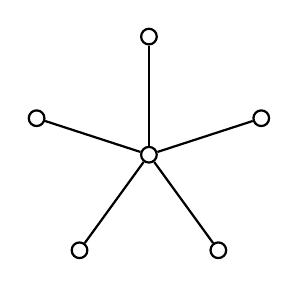
\begin{tikzpicture}
[nodeDecorate/.style={shape=circle,inner sep=2pt,draw,thick},%
  lineDecorate/.style={-,thick},%
  scale=1.5]
%% complete bipartite graph K_{1,5}
%% nodes or vertices
\foreach \nodename/\x/\y in {
  1/0.9510/0.3090, 2/0/1, 3/-0.9510/0.3090, 4/-0.5877/-0.8090,
  5/0.5877/-0.8090, 6/0/0}
{
  \node (\nodename) at (\x,\y) [nodeDecorate] {};
}
%% edges or lines
\path
\foreach \startnode/\endnode in {1/6, 2/6, 3/6, 4/6, 5/6}
{
  (\startnode) edge[lineDecorate] node {} (\endnode)
};
\end{tikzpicture}
}
%%
%%
\qquad
\subfigure[$|C(G)| = 2$]{
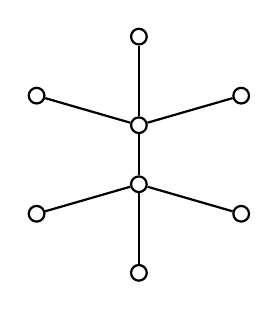
\begin{tikzpicture}
[nodedecorate/.style={shape=circle,inner sep=2pt,draw,thick},%
  linedecorate/.style={-,thick},%
  scale=1.5]
%% nodes or vertices
\foreach \nodename/\x/\y in {1/0.8660/0.5, 2/0/1, 3/-0.8660/0.5,
  4/-0.8660/-0.5, 5/0/-1, 6/0.8660/-0.5, 7/0/0.25, 8/0/-0.25}
{
  \node (\nodename) at (\x,\y) [nodedecorate] {};
}
%% edges or lines
\path
\foreach \startnode/\endnode in {7/1, 7/2, 7/3, 7/8, 8/4, 8/5, 8/6}
{
  (\startnode) edge[linedecorate] node {} (\endnode)
};
\end{tikzpicture}
}
%%
%%
\qquad
\subfigure[$|C(G)| = 3$]{
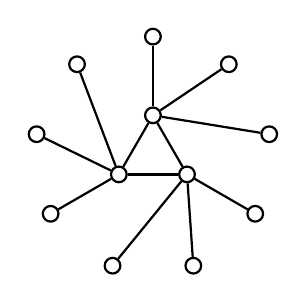
\begin{tikzpicture}
[nodedecorate/.style={shape=circle,inner sep=2pt,draw,thick},%
  linedecorate/.style={-,thick},%
  scale=1.5]
%% nodes or vertices
\foreach \nodename/\x/\y in {
  %% outer vertices
  1/0/1, 2/0.6427/0.7660, 3/0.9848/0.1736, 4/0.8660/-0.5,
  5/0.3420/-0.9396, 6/-0.3420/-0.9396, 7/-0.8660/-0.5,
  8/-0.9848/0.1736, 9/-0.6427/0.7660,
  %% inner vertices
  10/0/0.3333, 11/0.2886/-0.1666, 12/-0.2886/-0.1666}
{
  \node (\nodename) at (\x,\y) [nodedecorate] {};
}
%% edges or lines
\path
\foreach \startnode/\endnode in {
  10/1, 10/2, 10/3, 11/4, 11/5, 11/6, 12/7, 12/8, 12/9, 10/11, 11/12, 12/10}
{
  (\startnode) edge[linedecorate] node {} (\endnode)
};
\end{tikzpicture}
}
\end{figure}

\end{document}

\caption{Constructing graphs with arbitrarily large centers.}
\label{fig:distance_connectivity:graphs_arbitrarily_large_centers}
\end{figure}

\begin{theorem}
\textbf{Jordan~\cite{Jordan1869}.}
If a tree $T$ has order $\geq 3$, then the center of $T$ is either a
single vertex or two adjacent vertices.
\end{theorem}

\begin{proof}
As all eccentric vertices of $T$ are leaves~(see
problem~\ref{chap:distance_connectivity}.\ref{prob:distance_connectivity:eccentric_vertices_laves}),
removing all the leaves of $T$ decreases the eccentricities of the
remaining vertices by one. The tree comprised of the surviving
vertices has the same center as $T$. Continue pruning leaves as
described above and note that the tree comprised of the surviving
vertices has the same center as the previous tree. After a finite
number of leaf pruning stages, we eventually end up with a tree made
up of either one vertex or two adjacent vertices. The vertex set of
this final tree is the center of $T$.
\end{proof}


%%%%%%%%%%%%%%%%%%%%%%%%%%%%%%%%%%%%%%%%%%%%%%%%%%%%%%%%%%%%%%%%%%%%%%%%%%%

\subsection{Distance matrix}

In sections~\ref{sec:introduction:distance_matrix}
and~\ref{sec:graph_algorithms:weights_distances}, the distance matrix
$D$ of a graph $G$ was defined to be $D = [d_{ij}]$, where
$d_{ij} = d(v_i, v_j)$ and the vertices of $G$ are indexed by
$V = \{v_0, v_1, \dots, v_k\}$. The matrix $D$ is square where we set
$d_{ij} = 0$ for entries along the main diagonal. If there is no path
from $v_i$ to $v_j$, then we set $d_{ij} = \infty$. If $G$ is
undirected, then $D$ is symmetric and is equal to its transpose,
i.e. $D^T = D$. To compute the distance matrix $D$, apply the
Floyd-Roy-Warshall\index{Floyd-Roy-Warshall algorithm} algorithm to
determine the distances between all pairs of vertices. Refer to
Figure~\ref{fig:distance_connectivity:distance_matrix_directed_undirected_graphs}
for examples of distance matrices of directed and undirected
graphs. In the remainder of this section, ``graph'' refers to an
undirected graph unless otherwise specified.

\begin{figure}[!htbp]
\centering
\index{matrix!distance}
%%%%%%%%%%%%%%%%%%%%%%%%%%%%%%%%%%%%%%%%%%%%%%%%%%%%%%%%%%%%%%%%%%%%%%%%%%%
%% This file is part of the book
%%
%% Algorithmic Graph Theory
%% http://code.google.com/p/graph-theory-algorithms-book/
%%
%% Copyright (C) 2009, 2010, 2011 Minh Van Nguyen <nguyenminh2@gmail.com>
%%
%% See the file COPYING for copying conditions.
%%%%%%%%%%%%%%%%%%%%%%%%%%%%%%%%%%%%%%%%%%%%%%%%%%%%%%%%%%%%%%%%%%%%%%%%%%%

%% digraph
\subfigure[]{
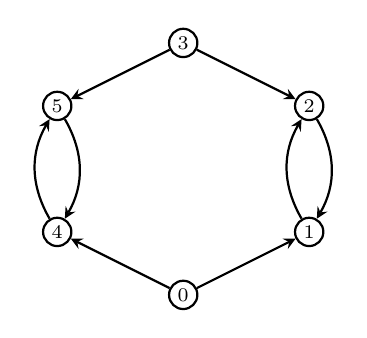
\begin{tikzpicture}
[arrowDecorate/.style={->,>=stealth,thick},%
  nodeDecorate/.style={shape=circle,inner sep=1.5pt,draw,thick},%
  scale=0.8]
\scriptsize
%% nodes or vertices
\foreach \nodename/\x/\y in {1/2/1, 2/2/3, 3/0/4, 0/0/0, 4/-2/1, 5/-2/3}
{
  \node (\nodename) at (\x,\y) [nodeDecorate] {$\nodename$};
}
%% edges or lines
\path
(1) edge[arrowDecorate,bend left] node {} (2)
(2) edge[arrowDecorate,bend left] node {} (1)
(3) edge[arrowDecorate] node {} (2)
(3) edge[arrowDecorate] node {} (5)
(0) edge[arrowDecorate] node {} (1)
(0) edge[arrowDecorate] node {} (4)
(4) edge[arrowDecorate,bend left] node {} (5)
(5) edge[arrowDecorate,bend left] node {} (4);
\end{tikzpicture}
%%
%%
\qquad\qquad
%%
%%
\begin{tikzpicture}
\node at (0,0) {%
$
\begin{bmatrix}
0      & 1      & 2      & \infty & 1      & 2 \\
\infty & 0      & 1      & \infty & \infty & \infty \\
\infty & 1      & 0      & \infty & \infty & \infty \\
\infty & 2      & 1      & 0      & 2      & 1 \\
\infty & \infty & \infty & \infty & 0      & 1 \\
\infty & \infty & \infty & \infty & 1      & 0
\end{bmatrix}
$
};
\end{tikzpicture}
}
%%
%%
\qquad
%% graph
\subfigure[]{
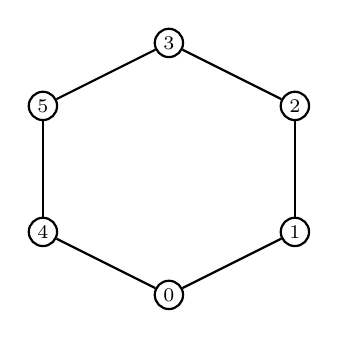
\begin{tikzpicture}
[lineDecorate/.style={-,thick},%
  nodeDecorate/.style={shape=circle,inner sep=1.5pt,draw,thick},%
  scale=0.8]
\scriptsize
%% nodes or vertices
\foreach \nodename/\x/\y in {1/2/1, 2/2/3, 3/0/4, 0/0/0, 4/-2/1, 5/-2/3}
{
  \node (\nodename) at (\x,\y) [nodeDecorate] {$\nodename$};
}
%% edges or lines
\path
\foreach \startnode/\endnode in {1/2, 1/0, 2/3, 3/5, 0/4, 4/5}
{
  (\startnode) edge[lineDecorate] node {} (\endnode)
};
\end{tikzpicture}
%%
%%
\qquad\qquad
%%
%%
\begin{tikzpicture}
\node at (0,0) {%
$
\begin{bmatrix}
0 & 1 & 2 & 3 & 1 & 2 \\
1 & 0 & 1 & 2 & 2 & 3 \\
2 & 1 & 0 & 1 & 3 & 2 \\
3 & 2 & 1 & 0 & 2 & 1 \\
1 & 2 & 3 & 2 & 0 & 1 \\
2 & 3 & 2 & 1 & 1 & 0
\end{bmatrix}
$
};
\end{tikzpicture}
}

\caption{Distance matrices of directed and undirected graphs.}
\label{fig:distance_connectivity:distance_matrix_directed_undirected_graphs}
\end{figure}

Instead of one distance matrix, we can define several distance
matrices on $G$. Consider an edge-weighted graph $G = (V,E)$ without
negative weight cycles and let
\[
d: V \times V \to \R \cup \{\infty\}
\]
be a distance function of $G$. Let $\partial = \diam(G)$ be the
diameter of $G$ and index the vertices of $G$ in some arbitrary but
fixed manner, say $V = \{v_0, v_1, \dots, v_n\}$. The sequence of
\emph{distance matrices}\index{matrix!distance} of $G$ are a sequence
of $(n - 1) \times (n - 1)$ matrices $A_1, A_2, \dots, A_\partial$ where
\[
(A_k)_{ij}
=
\begin{cases}
1, & \text{if $d(v_i, v_j) = k$}, \\[4pt]
0, & \text{otherwise}.
\end{cases}
\]
In particular, $A_1$ is the usual adjacency matrix $A$. To compute the
sequence of distance matrices of $G$, use the
Floyd-Roy-Warshall\index{Floyd-Roy-Warshall algorithm} algorithm to
compute the distance between each pair of vertices and assign the
resulting distance to the corresponding matrix $A_i$.

The distance matrix arises in several applications, including
communication network design~\cite{GrahamPollak1971} and network flow
algorithms~\cite{Dijkstra1959}. Thanks to
Graham\index{Graham, Ronald L.} and
Pollak\index{Pollak, O.}~\cite{GrahamPollak1971}, the following
unusual fact is known. If $T$ is any tree then
\[
\det D(T)
=
(-1)^{n - 1} (n - 1) 2^{n - 2}
\]
where $n$ denotes the order of $T$. In particular, the determinant of
the distance matrix of a tree is independent of the structure of the
tree.  This fact is proven in the paper~\cite{GrahamPollak1971}, but
see also~\cite{EdelbergEtAl1976}.


%%%%%%%%%%%%%%%%%%%%%%%%%%%%%%%%%%%%%%%%%%%%%%%%%%%%%%%%%%%%%%%%%%%%%%%%%%%

\section{Vertex and edge connectivity}

If $G = (V,E)$ is a graph and $U \subseteq V$ is a vertex set with the
property that $G - U$ has more connected components than $G$, then we
call $U$ a \emph{vertex-cut}\index{vertex-cut}. The term
\emph{cut-vertex}\index{cut-vertex} or
\emph{cut-point}\index{cut-point} is used when the vertex-cut consists
of exactly one vertex. For an intuitive appreciation of vertex-cut,
suppose $G = (V,E)$ is a connected graph. Then $U \subseteq V$ is a
vertex-cut if the vertex\index{vertex!deletion subgraph} deletion
subgraph $G - U$ is disconnected. For example, the cut-vertex of the
graph in Figure~\ref{fig:distance_connectivity:claw_graph} is the
vertex $0$. By $\kappa_v(G)$\index{$\kappa_v(G)$} we mean the
\emph{vertex connectivity}\index{vertex connectivity} of a connected
graph $G$, defined as the minimum number of vertices whose removal
would either disconnect $G$ or reduce $G$ to the trivial graph. The
vertex connectivity $\kappa_v(G)$ is also written as
$\kappa(G)$\index{$\kappa(G)$}. The vertex connectivity of the graph
in Figure~\ref{fig:distance_connectivity:claw_graph} is
$\kappa_v(G) = 1$ because we only need to remove vertex $0$ in order
to disconnect the graph. The vertex connectivity of a connected graph
$G$ is thus the vertex-cut of minimum cardinality. And $G$ is said to
be $k$-\emph{connected}\index{$k$-connected} if $\kappa_v(G) \geq k$.
From the latter definition, it immediately follows that if $G$ has at
least $3$ vertices and is $k$-connected then any vertex-cut of $G$ has
at least cardinality $k$. For instance, the graph in
Figure~\ref{fig:distance_connectivity:claw_graph} is $1$-connected. In
other words, $G$ is $k$-connected if the graph remains connected even
after removing any $k - 1$ or fewer vertices from $G$.

\begin{figure}[!htbp]
\centering
\index{cut-edge}
\index{cut-vertex}
\index{claw graph}
%%%%%%%%%%%%%%%%%%%%%%%%%%%%%%%%%%%%%%%%%%%%%%%%%%%%%%%%%%%%%%%%%%%%%%%%%%%
%% This file is part of the book
%%
%% Algorithmic Graph Theory
%% http://code.google.com/p/graph-theory-algorithms-book/
%%
%% Copyright (C) 2009, 2010, 2011 Minh Van Nguyen <nguyenminh2@gmail.com>
%%
%% See the file COPYING for copying conditions.
%%%%%%%%%%%%%%%%%%%%%%%%%%%%%%%%%%%%%%%%%%%%%%%%%%%%%%%%%%%%%%%%%%%%%%%%%%%

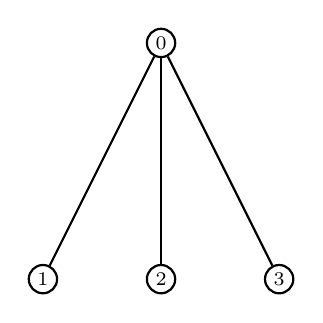
\begin{tikzpicture}
[nodeDecorate/.style={shape=circle,inner sep=1.5pt,draw,thick},%
  lineDecorate/.style={-,thick},%
  scale=1.5]
\scriptsize
%% nodes or vertices
\foreach \nodename/\x/\y in {1/0/0, 2/1/0, 3/2/0, 0/1/2}
{
  \node (\nodename) at (\x,\y) [nodeDecorate] {$\nodename$};
}
%% edges or lines
\path
\foreach \startnode/\endnode in {0/1, 0/2, 0/3} {
  (\startnode) edge[lineDecorate] node {} (\endnode)
};
\end{tikzpicture}

\caption{A claw graph with $4$ vertices.}
\label{fig:distance_connectivity:claw_graph}
\end{figure}

\begin{figure}[!htbp]
\centering
\index{Petersen!graph}
%%%%%%%%%%%%%%%%%%%%%%%%%%%%%%%%%%%%%%%%%%%%%%%%%%%%%%%%%%%%%%%%%%%%%%%%%%%
%% This file is part of the book
%%
%% Algorithmic Graph Theory
%% http://code.google.com/p/graph-theory-algorithms-book/
%%
%% Copyright (C) 2009, 2010, 2011 Minh Van Nguyen <nguyenminh2@gmail.com>
%%
%% See the file COPYING for copying conditions.
%%%%%%%%%%%%%%%%%%%%%%%%%%%%%%%%%%%%%%%%%%%%%%%%%%%%%%%%%%%%%%%%%%%%%%%%%%%

\documentclass{article}

\usepackage{tikz}
\usetikzlibrary{external}
\tikzexternalize{petersen-graph}

\begin{document}

\begin{figure}
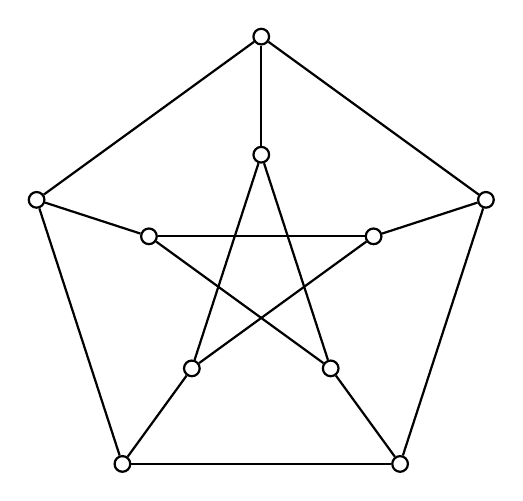
\begin{tikzpicture}
[nodeDecorate/.style={shape=circle,inner sep=2pt,draw,thick},%
  lineDecorate/.style={-,thick},scale=1.5]
%% nodes or vertices
\foreach \nodename/\x/\y in {
  %% outer pentagon
  0/0/2, 1/-1.9021/0.6180, 2/-1.1755/-1.6180, 3/1.1755/-1.6180,
  4/1.9021/0.6180,
  %% inner pentagon
  5/0/1, 6/-0.9510/0.3090, 7/-0.5877/-0.8090, 8/0.5877/-0.8090,
  9/0.9510/0.3090}
{
  \node (\nodename) at (\x,\y) [nodeDecorate] {};
}
%% edges or lines
\path
\foreach \startnode/\endnode in {0/1, 0/4, 0/5, 1/2, 1/6, 2/3, 2/7,
  3/4, 3/8, 4/9, 5/7, 5/8, 6/8, 6/9, 7/9}
{
  (\startnode) edge[lineDecorate] node {} (\endnode)
};
\end{tikzpicture}
\end{figure}

\end{document}

\caption{The Petersen graph on $10$ vertices.}
\label{fig:distance_connectivity:petersen_graph}
\end{figure}

\begin{example}
\rm
Here is a Sage example concerning $\kappa(G)$ using the
Petersen\index{Petersen!graph} graph depicted in
Figure~\ref{fig:distance_connectivity:petersen_graph}. A linear
programming Sage package, such as GLPK, must be installed for the
commands below to work.
%%
\begin{lstlisting}
sage: G = graphs.PetersenGraph()
sage: len(G.vertices())
10
sage: G.vertex_connectivity()
3.0
sage: G.delete_vertex(0)
sage: len(G.vertices())
9
sage: G.vertex_connectivity()
2.0
\end{lstlisting}
\qed
\end{example}

The notions of edge-cut and cut-edge are similarly defined. Let
$G = (V,E)$ be a graph and $D \subseteq E$ an edge set such that the
edge deletion subgraph $G - D$ has more components than $G$. Then $D$
is called an \emph{edge-cut}\index{edge-cut}. An edge-cut $D$ is said
to be \emph{minimal} if no proper subset of $D$ is an edge-cut. The
term \emph{cut-edge}\index{cut-edge} or \emph{bridge}\index{bridge} is
reserved for the case where the set $D$ is a singleton. Think of a
cut-edge as an edge whose removal from a connected graph would result
in that graph being disconnected. Going back to the case of the graph
in Figure~\ref{fig:distance_connectivity:claw_graph}, each edge of the
graph is a cut-edge. A graph having no cut-edge is called
\emph{bridgeless}\index{bridgeless}. An open question as of~2010
involving bridges is the
\emph{cycle double cover conjecture}\index{cycle double cover conjecture},
due to Paul Seymour\index{Seymour!Paul} and G.~Szekeres\index{Szekeres, G.},
which states that every bridgeless graph admits a set of cycles that
contains each edge exactly twice. The \emph{edge connectivity} of a
connected graph $G$, written $\kappa_e(G)$\index{$\kappa_e(G)$} and
sometimes denoted by $\lambda(G)$\index{$\lambda(G)$}, is the minimum
number of edges whose removal would disconnect $G$. In other words,
$\kappa_e(G)$ is the minimum cardinality among all edge-cuts of
$G$. Furthermore, $G$ is said to be
$k$-\emph{edge-connected}\index{$k$-edge-connected} if
$\kappa_e(G) \geq k$. A connected graph that is $k$-edge-connected is
guaranteed to be connected after removing $\leq k - 1$ edges from
it. When we have removed $k$ or more edges, then the graph would
become disconnected. By convention, a $1$-edge-connected graph is
simply a connected graph. The graph in
Figure~\ref{fig:distance_connectivity:claw_graph} has edge
connectivity $\kappa_e(G) = 1$ and is $1$-edge-connected.

\begin{example}
\rm
Here is a Sage example concerning $\lambda(G)$ using the
Petersen\index{Petersen!graph} graph shown in
Figure~\ref{fig:distance_connectivity:petersen_graph}. You must
install an optional linear programming Sage package such as GLPK for
the commands below to work.
%%
\begin{lstlisting}
sage: G = graphs.PetersenGraph()
sage: len(G.vertices())
10
sage: E = G.edges(); len(E)
15
sage: G.edge_connectivity()
3.0
sage: G.delete_edge(E[0])
sage: len(G.edges())
14
sage: G.edge_connectivity()
2.0
\end{lstlisting}
\qed
\end{example}

Vertex and edge connectivity are intimately related to the reliability
and survivability of computer networks. If a computer network
$G$~(which is a connected graph) is $k$-connected, then it would
remain connected despite the failure of at most $k - 1$ network
nodes. Similarly, $G$ is $k$-edge-connected if the network remains
connected after the failure of at most $k - 1$ network links. In
practical terms, a network with redundant nodes and/or links can
afford to endure the failure of a number of nodes and/or links and
still be connected, whereas a network with very few redundant nodes
and/or links~(e.g. something close to a spanning tree) is more prone
to be disconnected. A $k$-connected or $k$-edge-connected network is
more robust (i.e. can withstand) against node and/or link failures
than is a $j$-connected or $j$-edge-connected network, where $j < k$.

\begin{proposition}
\label{prop:distance_connectivity:edge_degree_inequality}
If $\delta(G)$ is the minimum degree of an undirected connected graph
$G = (V,E)$, then the edge connectivity of $G$ satisfies
$\lambda(G) \leq \delta(G)$.
\end{proposition}

\begin{proof}
Choose a vertex $v \in V$ whose degree is
$\deg(v) = \delta(G)$. Deleting the $\delta(G)$ edges incident on $v$
suffices to disconnect $G$ as $v$ is now an isolated vertex. It is
possible that $G$ has an edge-cut whose cardinality is smaller than
$\delta(G)$. Hence the result follows.
\end{proof}

Let $G = (V,E)$ be a graph and suppose $X_1$ and $X_2$ comprise a
partition of $V$. A \emph{partition-cut} of $G$, denoted
$\langle X_1, X_2 \rangle$, is the set of all edges of $G$ with one
endpoint in $X_1$ and the other endpoint in $X_2$. If $G$ is a
bipartite graph with bipartition $X_1$ and $X_2$, then
$\langle X_1, X_2 \rangle$ is a partition-cut of $G$. It follows that
a partition-cut is also an edge-cut.

\begin{proposition}
An undirected connected graph $G$ is $k$-edge-connected if and only if
any partition-cut of $G$ has at least $k$ edges.
\end{proposition}

\begin{proof}
Assume that $G$ is $k$-edge-connected. Then each edge-cut has at least
$k$ edges. As a partition-cut is an edge-cut, then any partition-cut
of $G$ has at least $k$ edges.

On the other hand, suppose each partition-cut has at least $k$
edges. If $D$ is a minimal edge-cut of $G$ and $X_1$ and $X_2$ are the
vertex sets of the two components of $G - D$, then
$D = \langle X_1, X_2 \rangle$. To see this, note that
$D \subseteq \langle X_1, X_2 \rangle$. If
$\langle X_1, X_2 \rangle - D \neq \emptyset$ then choose some
$e \in \langle X_1, X_2 \rangle$ such that $e \notin D$. The endpoints
of $e$ belong to the same component of $G - D$, in contradiction of
the definition of $X_1$ and $X_2$. Thus any minimal edge-cut is a
partition-cut and conclude that any edge-cut has at least $k$ edges.
\end{proof}

%% NOTE: need to polish up statement and proof of Bondy's theorem.
%% \begin{theorem}
%% (Bondy's theorem)
%% {\rm
%% Suppose

%% \begin{itemize}
%% \item
%% $G=(V,E)$ is a connected simple graph with $n=|V|$,
%% \item
%% $0<k<n$,
%% \item
%% the (non-decreasing) degree sequence
%% $[d_1,d_2,\dots, d_n]$ satisfies
%% $d_j\geq j+k-1$, for $1\leq j\leq n-1-d_{n-k+1}$,
%% \end{itemize}
%% then $G$ is $k$-vertex-connected.
%% }
%% \end{theorem}
%% \index{Bondy's theorem}

%% \begin{proof}[Solution]
%% Suppose not, so $\kappa(G)<k$. Then there exists an
%% $S\subset V$, $|S|=s<k$, such that $G'=G-S$ has more
%% than one connected component. Let $H$ be connected
%% component of $G'$ of minimal number of
%% vertices, $j=V(H)$. If $v\in V(H)$ then
%% $\deg_G(v)\leq j-1+s$, since $v$ is not adjacent to any
%% vertex in any other connected component of $G'$.

%% Since $H$ was chosen minimally, $j\leq n-s-j$, so
%% $\deg_G(v)\leq n-j-1$. This proves the following claim.

%% \noindent
%% {\bf Claim}: If $\deg_G(v) > n-j-1$ then $v\in S$.

%% A vertex of degree $d_{n-s}$ cannot belong to
%% $S$ because $S$ has $|S|=s$ vertices and the
%% vertices of degree $d_n$, $d_{n-1}$, \dots,
%% $d_{n-s-1}$ already exhaust the vertices in $S$. Therefore,

%% \[
%% d_{n-s}\leq n-j-1.
%% \]
%% We have $s\leq k-1$, so $d_{n-(k-1)}\leq d_{n-s}\leq n-j-1$,
%% so $j\leq n-1-d_{n-k+1}$.

%% Recall $v\in V(H)$ implies $\deg_G(v)\leq j-1+s$.
%% Since $j=|V(H)|$, we have
%% $d_j\leq j-1-s$.
%% By hypothesis, $d_j\geq j+k-1$, so together we have

%% \[
%% j+k-1\leq d_j \leq j-1+s.
%% \]
%% This forces $k\leq s$, a contradiction.
%% \end{proof}

\begin{proposition}
\label{prop:distance_connectivity:vertex_edge_inequality}
If $G = (V,E)$ is an undirected connected graph with vertex
connectivity $\kappa(G)$ and edge connectivity $\lambda(G)$, then we
have $\kappa(G) \leq \lambda(G)$.
\end{proposition}

\begin{proof}
Let $S$ be an edge-cut of $G$ with cardinality
$k = |S| = \lambda(G)$. Removing $k$ suitably chosen vertices of $G$
suffice to delete the edges of $S$ and hence disconnect $G$. It is
also possible to have a smaller vertex-cut elsewhere in $G$. Hence the
inequality follows.
\end{proof}

Taking together
Propositions~\ref{prop:distance_connectivity:edge_degree_inequality}
and~\ref{prop:distance_connectivity:vertex_edge_inequality}, we have
Whitney's\index{Whitney!inequality} inequality.

\begin{theorem}
\textbf{Whitney's inequality~\cite{Whitney1932}.}\index{Whitney!inequality}
Let $G$ be an undirected connected graph with vertex connectivity
$\kappa(G)$, edge connectivity $\lambda(G)$, and minimum degree
$\delta(G)$. Then we have the following inequality:
\[
\kappa(G)
\leq
\lambda(G)
\leq
\delta(G).
\]
\end{theorem}

\begin{proposition}
\label{prop:distance_connectivity:edge_removal_subgraph_k_minus_1_connected}
Let $G$ be an undirected connected graph that is $k$-connected for
some $k \geq 3$. If $e$ is an edge of $G$, then the edge-deletion
subgraph $G - e$ is $(k - 1)$-connected.
\end{proposition}

\begin{proof}
Let $V = \{v_1, v_2, \dots, v_{k-2}\}$ be a set of $k - 2$ vertices in
$G - e$. It suffice to show the existence of a $u$-$v$ walk in
$(G - e) - V$ for any distinct vertices $u$ and $v$ in
$(G - e) - V$. We need to consider two cases:~(i) at least one of the
endpoints of $e$ is in $V$; and~(ii) neither endpoints of $e$ is in
$V$.

(i)~Assume that $V$ has at least one endpoint of $e$. As $G - V$ is
$2$-connected, any distinct pair of vertices $u$ and $v$ in $G - V$ is
connected by a $u$-$v$ path that excludes $e$. Hence the $u$-$v$ path
is also in $(G - e) - V$.

(ii)~Assume that neither endpoints of $e$ is in $V$. If $u$ and $v$
are distinct vertices in $(G - e) - V$, then either:~(1) both $u$ and
$v$ are endpoints of $e$; or~(2) at least one of $u$ and $v$ is an
endpoint of $e$.
%%
\begin{enumerate}[(1)]
\item Suppose $u$ and $v$ are both endpoints of $e$. As $G$ is
  $k$-connected, then $G$ has at least $k + 1$ vertices so that the
  vertex set of $G - \{v_1, v_2, \dots, v_{k-2}, u, v\}$ is
  nonempty. Let $w$ be a vertex of
  $G - \{v_1, v_2, \dots, v_{k-2}, u, v\}$. Then there is a $u$-$w$
  path in $G - \{v_1, v_2, \dots, v_{k-2}, v\}$ and a $w$-$v$ path in
  $G - \{v_1, v_2, \dots, v_{k-2}, u\}$. Neither the $u$-$w$ nor the
  $w$-$v$ paths contain $e$. The concatenation of these two paths is a
  $u$-$v$ walk in $(G - e) - V$.

\item Now suppose at least one of $u$ and $v$, say $u$, is an endpoint
  of $e$. Let $w$ be the other endpoint of $e$. As $G$ is
  $k$-connected, then $G - \{v_1, v_2, \dots, v_{k-2}, w\}$ is
  connected and we can find a $u$-$v$ path $P$ in
  $G - \{v_1, v_2, \dots, v_{k-2}, w\}$. Furthermore $P$ is a $u$-$v$
  path in $G - \{v_1, v_2, \dots, v_{k-2}\}$ that neither contain $w$
  nor $e$. Hence $P$ is a $u$-$v$ path in $(G - e) - V$.
\end{enumerate}
%%
Conclude that $G - e$ is $(k - 1)$-connected.
\end{proof}

Repeated application of
Proposition~\ref{prop:distance_connectivity:edge_removal_subgraph_k_minus_1_connected}
results in the following corollary.

\begin{corollary}
Let $G$ be an undirected connected graph that is $k$-connected for
some $k \geq 3$. If $E$ is any set of $m$ edges of $G$, for
$m \leq k - 1$, then the edge-deletion subgraph $G - E$ is
$(k - m)$-connected.
\end{corollary}

What does it mean for a communications\index{communications network}
network to be fault-tolerant\index{fault-tolerant}? In~1932,
Hassler\index{Whitney!Hassler} Whitney provided~\cite{Whitney1932} a
characterization of $2$-connected graphs whereby he showed that a
graph $G$ is $2$-connected if and only if each pair of distinct
vertices in $G$ has two different paths connecting those two
vertices. A key to understanding Whitney's characterization of
$2$-connected graphs is the notion of internal vertex of a path. Given
a path $P$ in a graph, a vertex along that path is said to be an
\emph{internal vertex}\index{vertex!internal} if it is neither the
initial nor the final vertex of $P$. In other words, a path $P$ has an
internal vertex if and only if $P$ has at least two edges. Building
upon the notion of internal vertices, we now discuss what it means for
two paths to be internally disjoint. Let $u$ and $v$ be distinct
vertices in a graph $G$ and suppose $P_1$ and $P_2$ are two paths from
$u$ to $v$. Then $P_1$ and $P_2$ are said to be
\emph{internally disjoint}\index{path!internally disjoint} if they
do not share any common internal vertex. Two $u$-$v$ paths are
internally disjoint in the sense that both $u$ and $v$ are the only
vertices to be found in common between those paths. The notion of
internally disjoint paths can be easily extended to a collection of
$u$-$v$ paths. Whitney's characterization essentially says that a
graph is $2$-connected if and only if any two $u$-$v$ paths are
internally disjoint.

Consider the notion of internally disjoint paths within the context of
communications\index{communications network} network. As a first
requirement for fault-tolerant communications network, we want the
network to remain connected despite the failure of any network
node. By Whitney's characterization, this is possible if the original
communications network is $2$-connected. That is, we say that a
communications network is \emph{fault-tolerant}\index{fault-tolerant}
provided that any pair of distinct nodes is connected by two
internally disjoint paths. The failure of any node should at least
guarantee that any two distinct nodes are still connected.

\begin{theorem}
\label{thm:distance_connectivity:Whitney_characterization_2_connected_graphs}
\textbf{Whitney's characterization of $2$-connected graphs~\cite{Whitney1932}.}
Let $G$ be an undirected connected graph having at least $3$
vertices. Then $G$ is $2$-connected if and only if any two distinct
vertices in $G$ are connected by two internally disjoint paths.
\end{theorem}

\begin{proof}
($\Longleftarrow$)
For the case of necessity, argue by contraposition. That is, suppose
$G$ is not $2$-connected. Let $v$ be a cut-vertex of $G$, from which
it follows that $G - v$ is disconnected. We can find two vertices $w$
and $x$ such that there is no $w$-$x$ path in $G - v$. Therefore $v$
is an internal vertex of any $w$-$x$ path in $G$.

($\Longrightarrow$)
For the case of sufficiency, let $G$ be $2$-connected and let $u$ and
$v$ be any two distinct vertices in $G$. Argue by induction on
$d(u,v)$ that $G$ has at least two internally disjoint $u$-$v$
paths. For the base case, suppose $u$ and $v$ are connected by an edge
$e$ so that $d(u,v) = 1$. Adapt the proof of
Proposition~\ref{prop:distance_connectivity:edge_removal_subgraph_k_minus_1_connected}
to see that $G - e$ is connected. Hence we can find a $u$-$v$ path $P$
in $G - e$ such that $P$ and $e$ are two internally disjoint $u$-$v$
paths in $G$.

Assume for induction that $G$ has two internally disjoint $u$-$v$
paths where $d(u,v) < k$ for some $k \geq 2$. Let $w$ and $x$ be two
distinct vertices in $G$ such that $d(w,x) = k$ and hence there is a
$w$-$x$ path in $G$ of length $k$, i.e. we have a $w$-$x$ path
\[
W: w = w_1, w_2, \dots, w_{k-1}, w_k = x.
\]
Note that $d(w, w_{k-1}) < k$ and apply the induction hypothesis to
see that we have two internally disjoint $w$-$w_{k-1}$ paths in $G$;
call these paths $P$ and $Q$. As $G$ is $2$-connected, we have a
$w$-$x$ path $R$ in $G - w_{k-1}$ and hence $R$ is also a $w$-$x$ path
in $G$. Let $z$ be the vertex on $R$ that immediately precedes $x$ and
assume without loss of generality that $z$ is on $P$. We claim that
$G$ has two internally disjoint $w$-$x$ paths. One of these paths is
the concatenation of the subpath of $P$ from $w$ to $z$ with the
subpath of $R$ from $z$ to $x$. If $x$ is not on $Q$, then construct a
second $w$-$x$ path, internally disjoint from the first one, as
follows: concatenate the path $Q$ with the edge $w_{k-1} w$. In case
$x$ is on $Q$, take the subpath of $Q$ from $w$ to $x$ as the required
second path.
\end{proof}

From
Theorem~\ref{thm:distance_connectivity:Whitney_characterization_2_connected_graphs},
an undirected connected graph $G$ is $2$-connected if and only if any
two distinct vertices of $G$ are connected by two internally disjoint
paths. In particular, let $u$ and $v$ be any two distinct vertices of
$G$ and let $P$ and $Q$ be two internally disjoint $u$-$v$ paths as
guaranteed by
Theorem~\ref{thm:distance_connectivity:Whitney_characterization_2_connected_graphs}.
Starting from $u$, travel along the path $P$ to arrive at $v$. Then
start from $v$ and travel along the path $Q$ to arrive at $u$. The
concatenation of the internally disjoint paths $P$ and $Q$ is hence a
cycle passing through $u$ and $v$. We have proved the following
corollary to
Theorem~\ref{thm:distance_connectivity:Whitney_characterization_2_connected_graphs}.

\begin{corollary}
Let $G$ be an undirected connected graph having at least $3$
vertices. Then $G$ is $2$-connected if and only if any two distinct
vertices of $G$ lie on a common cycle.
\end{corollary}

The following theorem provides further characterizations of
$2$-connected graphs, in addition to Whitney's characterization.

\begin{theorem}
\label{thm:distance_connectivity:characterization_2_connected_graphs}
\textbf{Characterizations of $2$-connected graphs.}
Let $G = (V,E)$ be an undirected connected graph having at least $3$
vertices. Then the following are equivalent.
%%
\begin{enumerate}
\item $G$ is $2$-connected.

\item If $u,v \in V$ are distinct vertices of $G$, then $u$ and $v$
  lie on a common cycle.

\item If $v \in V$ and $e \in E$, then $v$ and $e$ lie on a common
  cycle.

\item If $e_1, e_2 \in E$ are distinct edges of $G$, then $e_1$ and
  $e_2$ lie on a common cycle.

\item If $u,v \in V$ are distinct vertices and $e \in E$, then they
  lie on a common path.

\item If $u,v,w \in V$ are distinct vertices, then they lie on a
  common path.

\item If $u,v,w \in V$ are distinct vertices, then there is a path
  containing any two of these vertices but excluding the third.
\end{enumerate}
\end{theorem}


%%%%%%%%%%%%%%%%%%%%%%%%%%%%%%%%%%%%%%%%%%%%%%%%%%%%%%%%%%%%%%%%%%%%%%%%%%%

\section{Menger's theorem}
\index{Menger's theorem}

Menger's theorem has a number of different versions: an undirected,
vertex-connectivity version; a directed, vertex-connectivity version;
an undirected, edge-connectivity version; and a directed,
edge-connectivity version. In this section, we will prove the
undirected, vertex-connectivity version. But first, let's consider a
few technical results that will be of use for the purpose of this
section.

Let $u$ and $v$ be distinct vertices in a connected graph $G = (V,E)$
and let $S \subseteq V$. Then $S$ is said to be $u$-$v$
\emph{separating} if $u$ and $v$ lie in different components of the
vertex deletion subgraph $G - S$. The vertices $u$ and $v$ are
positioned such that after removing vertices in $S$ from $G$ and the
corresponding edges, $u$ and $v$ are no longer connected nor strongly
connected to each other. It is clear by definition that
$u,v \notin S$. We also say that $S$ \emph{separates} $u$ and
$v$, or $S$ is a vertex separating set. Similarly an edge set
$T \subseteq E$ is $u$-$v$ separating~(or separates $u$ and $v$) if
$u$ and $v$ lie in different components of the edge deletion subgraph
$G - T$. But unlike the case of vertex separating sets, it is possible
for $u$ and $v$ to be endpoints of edges in $T$ because the removal of
edges does not result in deleting the corresponding endpoints. The set
$T$ is also called an edge separating set. In other words, $S$ is a
vertex cut\index{vertex!cut} and $T$ is an edge
cut\index{edge!cut}. When it is clear from context, we simply refer to
a separating\index{separating set} set. See
Figure~\ref{fig:distance_connectivity:vertex_edge_separating_sets} for
illustrations of separating sets.

\begin{figure}[!htbp]
\centering
\index{separating set}
%%%%%%%%%%%%%%%%%%%%%%%%%%%%%%%%%%%%%%%%%%%%%%%%%%%%%%%%%%%%%%%%%%%%%%%%%%%
%% This file is part of the book
%%
%% Algorithmic Graph Theory
%% http://code.google.com/p/graph-theory-algorithms-book/
%%
%% Copyright (C) 2009, 2010, 2011 Minh Van Nguyen <nguyenminh2@gmail.com>
%%
%% See the file COPYING for copying conditions.
%%%%%%%%%%%%%%%%%%%%%%%%%%%%%%%%%%%%%%%%%%%%%%%%%%%%%%%%%%%%%%%%%%%%%%%%%%%

\subfigure[Original graph.]{
\label{fig:separating_set:original_graph}
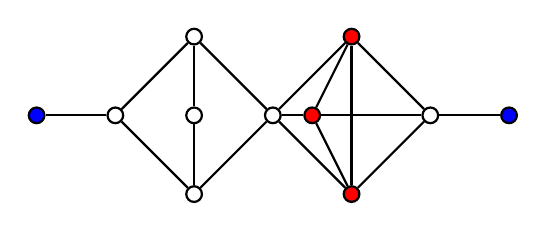
\begin{tikzpicture}
[nodeDecorate/.style={shape=circle,inner sep=2pt,draw,thick},%
  lineDecorate/.style={-,thick},scale=1]
%% nodes or vertices
\foreach \nodename/\x/\y in {
  0/0/0, 2/2/0, 6/-1/1, 7/-1/0, 8/-1/-1, 9/-2/0}
{
  \node (\nodename) at (\x,\y) [nodeDecorate] {};
}
\foreach \nodename/\x/\y/\fillcolor in {
  1/0.5/0/red, 3/3/0/blue, 4/1/-1/red, 5/1/1/red, 10/-3/0/blue}
{
  \node (\nodename) at (\x,\y) [nodeDecorate,fill=\fillcolor] {};
}
%% edges or lines
\path
\foreach \startnode/\endnode in {
  0/1, 0/4, 0/5, 0/6, 0/8, 1/2, 1/4, 1/5, 2/3, 2/4, 2/5, 4/5, 6/7,
  6/9, 7/8, 8/9, 9/10}
{
  (\startnode) edge[lineDecorate] node {} (\endnode)
};
\end{tikzpicture}
}
%%
%%
\qquad
\subfigure[Vertex separated.]{
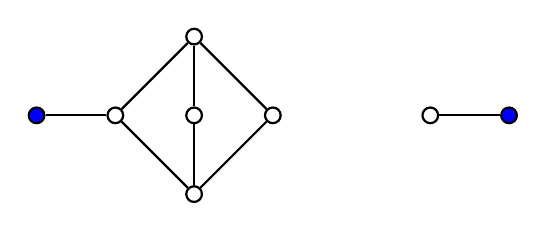
\begin{tikzpicture}
[nodeDecorate/.style={shape=circle,inner sep=2pt,draw,thick},%
  lineDecorate/.style={-,thick},scale=1]
%% nodes or vertices
\foreach \nodename/\x/\y in {
  0/0/0, 2/2/0, 6/-1/1, 7/-1/0, 8/-1/-1, 9/-2/0}
{
  \node (\nodename) at (\x,\y) [nodeDecorate] {};
}
\node (3) at (3,0) [nodeDecorate,fill=blue] {};
\node (10) at (-3,0) [nodeDecorate,fill=blue] {};
%% edges or lines
\path
\foreach \startnode/\endnode in {
  0/6, 0/8, 2/3, 6/7, 6/9, 7/8, 8/9, 9/10}
{
  (\startnode) edge[lineDecorate] node {} (\endnode)
};
\end{tikzpicture}
}
%%
%%
\subfigure[Original graph.]{
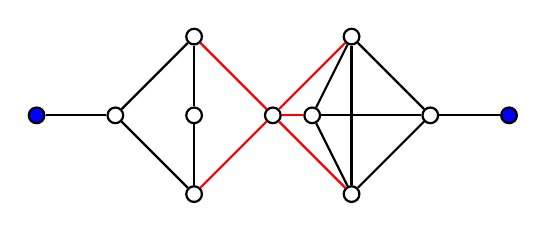
\begin{tikzpicture}
[nodeDecorate/.style={shape=circle,inner sep=2pt,draw,thick},%
  lineDecorate/.style={-,thick},scale=1]
%% nodes or vertices
\foreach \nodename/\x/\y in {
  0/0/0, 1/0.5/0, 2/2/0, 4/1/-1, 5/1/1, 6/-1/1, 7/-1/0, 8/-1/-1, 9/-2/0}
{
  \node (\nodename) at (\x,\y) [nodeDecorate] {};
}
\node (3) at (3,0) [nodeDecorate,fill=blue] {};
\node (10) at (-3,0) [nodeDecorate,fill=blue] {};
%% edges or lines
\path
\foreach \startnode/\endnode in {
  1/2, 1/4, 1/5, 2/3, 2/4, 2/5, 4/5, 6/7, 6/9, 7/8, 8/9, 9/10}
{
  (\startnode) edge[lineDecorate] node {} (\endnode)
}
\foreach \startnode/\endnode/\edgecolor in { 0/1, 0/4, 0/5, 0/6, 0/8}
{
  (\startnode) edge[lineDecorate,color=red] node {} (\endnode)
};
\end{tikzpicture}
}
%%
%%
\qquad
\subfigure[Edge separated.]{
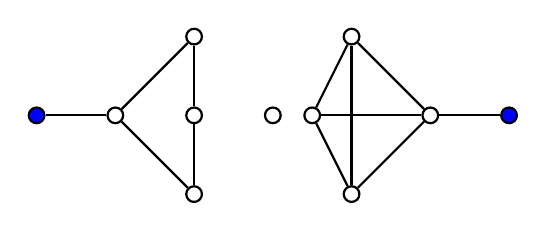
\begin{tikzpicture}
[nodeDecorate/.style={shape=circle,inner sep=2pt,draw,thick},%
  lineDecorate/.style={-,thick},scale=1]
%% nodes or vertices
\foreach \nodename/\x/\y in {
  0/0/0, 1/0.5/0, 2/2/0, 4/1/-1, 5/1/1, 6/-1/1, 7/-1/0, 8/-1/-1, 9/-2/0}
{
  \node (\nodename) at (\x,\y) [nodeDecorate] {};
}
\node (3) at (3,0) [nodeDecorate,fill=blue] {};
\node (10) at (-3,0) [nodeDecorate,fill=blue] {};
%% edges or lines
\path
\foreach \startnode/\endnode in {
  1/2, 1/4, 1/5, 2/3, 2/4, 2/5, 4/5, 6/7, 6/9, 7/8, 8/9, 9/10}
{
  (\startnode) edge[lineDecorate] node {} (\endnode)
};
\end{tikzpicture}
}

\caption{Vertex and edge separating sets. Blue-colored vertices are
  those we want to separate. The red-colored vertices form a vertex
  separating set or vertex cut\index{vertex!cut}; the red-colored
  edges constitute an edge separating set or edge cut\index{edge!cut}.}
\label{fig:distance_connectivity:vertex_edge_separating_sets}
\end{figure}

\begin{proposition}
\label{prop:distance_connectivity:upper_bound_internally_disjoint_paths}
Consider two distinct, non-adjacent vertices $u,v$ in a connected
graph $G$. If $\cP_{uv}$ is a collection of internally disjoint
$u$-$v$ paths in $G$ and $S_{uv}$ is a $u$-$v$ separating set of
vertices in $G$, then
%%
\begin{equation}
\label{eqn:distance_connectivity:upper_bound_internally_disjoint_paths}
|\cP_{uv}| \leq |S_{uv}|.
\end{equation}
\end{proposition}

\begin{proof}
Each $u$-$v$ path in $\cP_{uv}$ must include at least one vertex from
$S_{uv}$ because $S_{uv}$ is a vertex cut of $G$. Any two distinct
paths in $\cP_{uv}$ cannot contain the same vertex from $S_{uv}$. Thus
the number of internally disjoint $u$-$v$ paths is at most $|S_{uv}|$.
\end{proof}

The
bound~\eqref{eqn:distance_connectivity:upper_bound_internally_disjoint_paths}
holds for any $u$-$v$ separating set $S_{uv}$ of vertices in $G$. In
particular, we can choose $S_{uv}$ to be of minimum cardinality among
all $u$-$v$ separating sets of vertices in $G$. Thus we have the
following corollary. Menger's\index{Menger's theorem}
Theorem~\ref{thm:distance_connectivity:Menger_theorem} provides a much
stronger statement of
Corollary~\ref{cor:distance_connectivity:upper_bound_internally_disjoint_paths},
saying in effect that the two quantities $\max(|\cP_{uv}|)$ and
$\min(|S_{uv}|)$ are equal.

\begin{corollary}
\label{cor:distance_connectivity:upper_bound_internally_disjoint_paths}
Consider any two distinct, non-adjacent vertices $u,v$ in a connected
graph $G$. Let $\max(|\cP_{uv}|)$ be the maximum number of internally
disjoint $u$-$v$ paths in $G$ and denote by $\min(|S_{uv}|)$ the
minimum cardinality of a $u$-$v$ separating set of vertices in
$G$. Then we have $\max(|\cP_{uv}|) \leq \min(|S_{uv}|)$.
\end{corollary}

\begin{corollary}
Consider any two distinct, non-adjacent vertices $u,v$ in a connected
graph $G$. Let $\cP_{uv}$ be a collection of internally disjoint
$u$-$v$ paths in $G$ and let $S_{uv}$ be a $u$-$v$ separating set of
vertices in $G$. If $|\cP_{uv}| = |S_{uv}|$, then $\cP_{uv}$ has
maximum cardinality among all collections of internally disjoint
$u$-$v$ paths in $G$ and $S_{uv}$ has minimum cardinality among all
$u$-$v$ separating sets of vertices in $G$.
\end{corollary}

\begin{proof}
Argue by contradiction. Let $\cQ_{uv}$ be another collection of
internally disjoint $u$-$v$ paths in $G$ such that
$|\cQ_{uv}| \geq |\cP_{uv}|$. Then
$|\cP_{uv}| \leq |\cQ_{uv}| \leq |S_{uv}|$ by
Proposition~\ref{prop:distance_connectivity:upper_bound_internally_disjoint_paths}.
We cannot have $|\cQ_{uv}| > |\cP_{uv}|$, which would be contradictory
to our hypothesis that $\cP_{uv} = |S_{uv}|$. Thus
$|\cQ_{uv}| = |\cP_{uv}|$. Let $T_{uv}$ be another $u$-$v$
separating set of vertices in $G$ such that
$|T_{uv}| \leq |S_{uv}|$. Then we have
$|\cP_{uv}| \leq |T_{uv}| \leq |S_{uv}|$ by
Proposition~\ref{prop:distance_connectivity:upper_bound_internally_disjoint_paths}.
We cannot have $|T_{uv}| < |S_{uv}|$ because we would then end up with
$|\cP_{uv}| \leq |T_{uv}|$ and $\cP_{uv} = |S_{uv}|$, a
contradiction. Therefore $|T_{uv}| = |S_{uv}|$.
\end{proof}

\begin{lemma}
Consider two distinct, non-adjacent vertices $u,v$ in a connected
graph $G$ and let $k$ be the minimum number of vertices required to
separate $u$ and $v$. If $G$ has a $u$-$v$ path of length $2$, then
$G$ has $k$ internally disjoint $u$-$v$ paths.
\end{lemma}

\begin{proof}
Argue by induction on $k$. For the base case, assume $k = 1$. Hence
$G$ has a cut vertex $x$ such that $u$ and $v$ are disconnected in
$G - x$. Any $u$-$v$ path must contain $x$. In particular, there can
be only one internally disjoint $u$-$v$ path.

Assume for induction that $k \geq 2$. Let $P: u,x,v$ be a path in $G$
having length $2$ and suppose $S$ is a smallest $u$-$v$ separating set
for $G - x$. Then $S \cup \{x\}$ is a $u$-$v$ separating set for
$G$. By the minimality of $k$, we have $|S| \geq k - 1$. By the
induction hypothesis, we have at least $k - 1$ internally disjoint
$u$-$v$ paths in $G - x$. As $P$ is internally disjoint from any of
the latter paths, conclude that $G$ has $k$ internally disjoint
$u$-$v$ paths.
\end{proof}

\begin{theorem}
\label{thm:distance_connectivity:Menger_theorem}
\textbf{Menger's theorem.}\index{Menger's theorem}
Let $G$ be an undirected connected graph and let $u$ and $v$ be
distinct, non-adjacent vertices of $G$. Then the maximum number of
internally disjoint $u$-$v$ paths in $G$ equals the minimum number of
vertices needed to separate $u$ and $v$.
\end{theorem}

\begin{proof}
Suppose that the maximum number of independent $u$-$v$ paths in
$G$ is attained by $u$-$v$ paths $P_1$, \dots, $P_k$.
To obtain a separating set $W\subset V$, we must at least remove
one point in each path $P_i$. This implies
the minimum number of vertices needed to separate $u$ and $v$
is at least $k$. Therefore, we have an upper bound:

\[
\#\{ {\rm indep.}\ u-v\ {\rm paths}\}
\leq
\# \{{\rm min.\ number \ of\ vertices\ needed\ to\ separate}\ u\
{\rm and}\  v\}.
\]

We show that equality holds. Let $n$ denote the number
of edges of $G$. The proof is by induction on $n$. By hypothesis,
$n\geq 2$.
If $n=2$ the statement holds by inspection, since in that case
$G$ is a line graph with $3$ vertices
$V=\{u,v,w\}$ and $2$ edges, $E=\{uw.wv\}$. In that situation,
there is only $1$ $u$-$v$ path
(namely, $uwv$) and only one vertex separating $u$ and $v$
(namely, $w$).

Suppose now $n>3$ and assume the statement holds for each
graph with $<n$ edges. Let

\[
k = \#\{ {\rm independent}\ u-v\ {\rm paths}\}
\]
and let
\[
\ell =
\# \{{\rm min.\ number \ of\ vertices\ needed\ to\ separate}\
u\ {\rm and}\  v\},
\]
so that $k\leq \ell$. Let $e\in E$ and let $G/e$ be the
contraction graph having edges $E-\{e\}$ and
vertices the same as those of $G$, except that
the endpoints of $e$ have been identified.

Suppose that $k<\ell$ and $G$ does not have $\ell$
independent $u$-$v$ paths. The contraction
graph $G/e$ does not have $\ell$
independent $u$-$v$ paths either (where
now, if $e$ contains $u$ or $v$ then we must
appropriately redefine $u$ or $v$, if needed).
However, by the induction hypothesis
$G/e$ does have the property that
the maximum number of internally disjoint $u$-$v$ paths
equals the minimum number of vertices needed to separate $u$ and $v$.
Therefore,

\[
\begin{array}{c}
\#\{ {\rm independent}\ u-v\ {\rm paths\ in}\ G/e\}\\
<
\# \{{\rm min.\ number \ of\ vertices\ needed\ to\ separate}
\ u\ {\rm and}\  v\ {\rm in}\ G\}.
\end{array}
\]
By induction,

\[
\begin{array}{c}
\#\{ {\rm independent\ }u-v{\rm \ paths\ in\ }G/e\}\\
=
\# \{{\rm min.\ number \ of\ vertices\ needed\ to\ separate\
}u{\rm \ and}\  v\ {\rm in\ }G/e\}.
\end{array}
\]

Now, we {\it claim} we can pick $e$ such that $e$ does contain $u$ or $v$
and in such a way that

\[
\begin{array}{c}
\# \{{\rm minimum\ number \ of\ vertices\ needed\ to\ separate\ }u\
{\rm and\  }v\ {\rm in\ }G\}\\
\geq
\# \{{\rm minimum\ number \ of\ vertices\ needed\ to\ separate\ }u\
{\rm and\  }v\ {\rm in}\ G/e\}.
\end{array}
\]
Proof: Indeed, since $n>3$ any separating set realizing
the minimum number  of vertices needed to separate $u$ and
$v$ in $G$ cannot contain both a vertex in $G$ adjacent to $u$ and a vertex in
$G$ adjacent to $v$. Therefore, we may pick $e$ accordingly.
(Q.E.D. claim)

The result follows from the claim and the above inequalities.
\end{proof}

The following statement
is the undirected, edge-connectivity version of
Menger's theorem.

\begin{theorem}
\textbf{Menger's theorem (edge-connectivity form).}
{\rm
Let $G$ be an undirected graph, and let $s$ and $t$ be vertices in
$G$.
Then, the maximum number of edge-disjoint $(s,t)$-paths in
$G$
equals the minimum number of edges from $E(G)$ whose
deletion separates $s$ and $t$.
}
\end{theorem}

This is proven the same way as the previous version
but using the generalized min-cut/max-flow theorem (see
Remark \ref{remark:GMCMF} above).

\begin{theorem}
\textbf{Dirac's theorem.}\index{Dirac's theorem}
Let $G = (V,E)$ be an undirected $k$-connected graph with
$|V| \geq k + 1$ vertices for $k \geq 3$. If $S \subseteq V$ is any
set of $k$ vertices, then $G$ has a cycle containing the vertices of
$S$.
\end{theorem}

\begin{proof}
\end{proof}


%%%%%%%%%%%%%%%%%%%%%%%%%%%%%%%%%%%%%%%%%%%%%%%%%%%%%%%%%%%%%%%%%%%%%%%%%%%

\section{Whitney's Theorem}
\index{Whitney!theorem}

\begin{theorem}
\textbf{Whitney's theorem (vertex version).}
{\rm
Suppose $G=(V,E)$ is a graph with $|V|\geq k+1$. The following are
equivalent:
\begin{itemize}
\item
$G$ is $k$-vertex-connected,
\item
Any pair of distinct vertices $v,w\in V$ are connected by
at least $k$ independent paths.
\end{itemize}
}
\end{theorem}

\begin{proof}[Solution]

...

\end{proof}



\begin{theorem}
\textbf{Whitney's theorem (edge version).}
{\rm
Suppose $G=(V,E)$ is a graph with $|V|\geq k+1$. The following are
equivalent:
\begin{itemize}
\item
the graph $G$ is $k$-edge-connected,

\item
any pair of
vertices are connected by at least $k$ edge-disjoint paths.
\end{itemize}
}
\end{theorem}

\begin{proof}[Solution]

...

\end{proof}


\begin{theorem}
\textbf{Whitney's Theorem.}
Let $G = (V, E)$ be a connected graph such that $|V| \geq 3$. Then $G$
is $2$-connected if and only if any pair $u,v \in V$ has two
internally disjoint paths between them.
\end{theorem}


%%%%%%%%%%%%%%%%%%%%%%%%%%%%%%%%%%%%%%%%%%%%%%%%%%%%%%%%%%%%%%%%%%%%%%%%%%%

\section{Centrality of a vertex}

\begin{quote}
\footnotesize
Louis, I think this is the beginning of a beautiful friendship. \\
\noindent
--- Rick from the 1942 film \emph{Casablanca}
\end{quote}

\begin{itemize}
\item degree centrality

\item betweenness centrality

\item closeness centrality

\item eigenvector centrality
\end{itemize}

\begin{algorithm}[!htbp]
\index{friendship graph}
%%%%%%%%%%%%%%%%%%%%%%%%%%%%%%%%%%%%%%%%%%%%%%%%%%%%%%%%%%%%%%%%%%%%%%%%%%%
%% This file is part of the book
%%
%% Algorithmic Graph Theory
%% http://code.google.com/p/graph-theory-algorithms-book/
%%
%% Copyright (C) 2009, 2010 Minh Van Nguyen <nguyenminh2@gmail.com>
%%
%% See the file COPYING for copying conditions.
%%%%%%%%%%%%%%%%%%%%%%%%%%%%%%%%%%%%%%%%%%%%%%%%%%%%%%%%%%%%%%%%%%%%%%%%%%%

\DontPrintSemicolon
\SetAlgoNoLine
%%
%% data section
\SetKwInOut{Input}{Input}
\SetKwInOut{Output}{Output}
%%
%% input/output
\Input{A positive integer $n$.}
\Output{An edge list $E$ containing the edges of the friendship graph
  $F_n$.}
\BlankLine
%%
%% algorithm body
\If{$n = 1$}{
  \Return $C_3$\;
}
$E \assign [\,]$\;
$N \assign 2n + 1$\;
\For{$i \assign 0, 1, \dots, N-3$}{
  \eIf{\rm $i$ is odd}{
    append to $E$ the edges $(i,\, i+1)$ and $(i,\, N-1)$\;
  }{
    append to $E$ the edge $(i, N-1)$\;
  }
}
append to $E$ the edges $(N-2,\, 0)$ and $(N-2,\, N-1)$\;
\Return $E$\;

\caption{Friendship graph.}
\label{alg:distance_connectivity:friendship_graphs}
\end{algorithm}


%%%%%%%%%%%%%%%%%%%%%%%%%%%%%%%%%%%%%%%%%%%%%%%%%%%%%%%%%%%%%%%%%%%%%%%%%%%

\section{Network reliability}

\begin{itemize}
\item Whitney synthesis

\item Tutte's synthesis of $3$-connected graphs

\item Harary graphs

\item constructing an optimal $k$-connected $n$-vertex graph
\end{itemize}


%%%%%%%%%%%%%%%%%%%%%%%%%%%%%%%%%%%%%%%%%%%%%%%%%%%%%%%%%%%%%%%%%%%%%%%%%%%

\section{Problems}

\begin{quote}
\footnotesize
When you don't share your problems, you resent hearing the problems of
other people. \\
\noindent
--- Chuck Palahniuk, \emph{Invisible Monsters}, 1999
\end{quote}

\begin{problem}
\item Let $G = (V,E)$ be an undirected, unweighted simple graph. Show
  that $V$ and the distance\index{distance!function} function on $G$
  form a metric space if and only if $G$ is connected.

\item Let $u$ and $v$ be two distinct vertices in the same connected
  component of $G$. If $P$ is a $u$-$v$ path such that
  $d(u,v) = \epsilon(u)$, we say that $P$ is an
  \emph{eccentricity path}\index{eccentricity!path} for $u$.
  %%
  \begin{enumerate}[(a)]
  \item If $r$ is the root of a tree, show that the end-vertex of an
    eccentricity path for $r$ is a leaf.

  \item If $v$ is a vertex of a tree distinct from the root $r$, show
    that any eccentricity path for $v$ must contain $r$ or provide an
    example to the contrary.

  \item A vertex $w$ is said to be an
    \emph{eccentric vertex}\index{eccentricity!vertex} of $v$ if
    $d(v,w) = \epsilon(v)$. Intuitively, an eccentric vertex of $v$
    can be considered as being as far away from $v$ as possible. If
    $w$ is an eccentric vertex of $v$ and vice versa, then $v$ and $w$
    are said to be
    \emph{mutually eccentric}\index{eccentricity!mutual}. See Buckley
    and Lau~\cite{BuckleyLau2003} for detailed discussions of mutual
    eccentricity. If $w$ is an eccentric vertex of $v$, explain why
    $v$ is also an eccentric vertex of $w$ or show that this does not
    in general hold.
  \end{enumerate}

\item If $u$ and $v$ are vertices of a connected graph $G$ such that
  $d(u,v) = \diam(G)$, show that $u$ and $v$ are mutually eccentric.

\item If $uv$ is an edge of a tree $T$ and $w$ is a vertex of $T$
  distinct from $u$ and $v$, show that $|d(u,w) - d(w,v)| = W(uv)$
  with $W(uv)$ being the weight of $uv$.

\item If $u$ and $v$ are vertices of a tree $T$ such that
  $d(u,v) = \diam(T)$, show that $u$ and $v$ are leaves.

\item Let $v_1, v_2, \dots, v_k$ be the leaves of a tree $T$. Show
  that $\per(T) = \{v_1, v_2, \dots, v_k\}$.

\item\label{prob:distance_connectivity:eccentric_vertices_laves} Show
  that all the eccentric vertices of a tree are leaves.

\item If $G$ is a connected graph, show that
  $\radius(G) \leq \diam(G) \leq 2 \cdot \radius(G)$.

\item Let $T$ be a tree of order $\geq 3$. If the center of $T$ has
  one vertex, show that $\diam(T) = 2 \cdot \radius(T)$. If the center
  of $T$ has two vertices, show that
  $\diam(T) = 2 \cdot \radius(T) - 1$.

\item Let $G = (V,E)$ be a simple undirected, connected graph. Define
  the distance of a vertex $v \in V$ by
  \[
  d(v)
  =
  \sum_{x \in V} d(v,x)
  \]
  and define the distance of the graph $G$ itself by
  \[
  d(G)
  =
  \frac{1}{2} \sum_{v \in V} d(v).
  \]
  For any vertex $v \in V$, show that
  $d(G) \leq d(v) + d(G - v)$ with $G - v$ being a vertex deletion
  subgraph of $G$. This result appeared in
  Entringer~et~al.~\cite[p.284]{EntringerEtAl1976}.

\item Determine the sequence of distance matrices for the graphs in
  Figure~\ref{fig:distance_connectivity:distance_matrix_directed_undirected_graphs}.

\item If $G = (V,E)$ is an undirected connected graph and $v \in V$,
  prove the following vertex connectivity inequality:
  \[
  \kappa(G) - 1
  \leq
  \kappa(G - v)
  \leq
  \kappa(G).
  \]

\item If $G = (V,E)$ is an undirected connected graph and $e \in E$,
  prove the following edge connectivity inequality:
  \[
  \lambda(G) - 1
  \leq
  \lambda(G - e)
  \leq
  \lambda(G).
  \]

\begin{table}[!htbp]
\centering
\index{wine}
%%%%%%%%%%%%%%%%%%%%%%%%%%%%%%%%%%%%%%%%%%%%%%%%%%%%%%%%%%%%%%%%%%%%%%%%%%%
%% This file is part of the book
%%
%% Algorithmic Graph Theory
%% http://code.google.com/p/graph-theory-algorithms-book/
%%
%% Copyright (C) 2009, 2010, 2011 Minh Van Nguyen <nguyenminh2@gmail.com>
%%
%% See the file COPYING for copying conditions.
%%%%%%%%%%%%%%%%%%%%%%%%%%%%%%%%%%%%%%%%%%%%%%%%%%%%%%%%%%%%%%%%%%%%%%%%%%%

\footnotesize
\begin{tabular}{rl|rl|rl} \hline
code & name & code & name & code & name \\\hline
0 & Alicante Bouschet & 1 & Aramon & 2 & Bequignol \\
3 & Cabernet Franc & 4 & Cabernet Sauvignon & 5 & Carignan \\
6 & Chardonnay & 7 & Chenin Blanc & 8 & Colombard \\
9 & Donzillinho & 10 & Ehrenfelser & 11 & Fer Servadou \\
12 & Flora & 13 & Gamay & 14 & Gelber Ortlieber \\
15 & Gr\"uner Veltliner & 16 & Kemer & 17 & Merlot \\
18 & Meslier-Saint-Francois & 19 & M\"uller-Thurgau & 20 & Muscat Blanc \\
21 & Muscat Hamburg & 22 & Muscat of Alexandria & 23 & Optima \\
24 & Ortega & 25 & Osteiner & 26 & P\'eagudo \\
27 & Perle & 28 & Perle de Csaba & 29 & Perlriesling \\
30 & Petit Manseng & 31 & Petite Bouschet & 32 & Pinot Noir \\
33 & Reichensteiner & 34 & Riesling & 35 & Rotberger \\
36 & Roter Veltliner & 37 & Rotgipfler & 38 & Royalty \\
39 & Ruby Cabernet & 40 & Sauvignon Blanc & 41 & Sch\"onburger \\
42 & Semillon & 43 & Siegerrebe & 44 & Sylvaner \\
45 & Taminga & 46 & Teinturier du Cher & 47 & Tinta Madeira \\
48 & Traminer & 49 & Trincadeiro & 50 & Trollinger \\
51 & Trousseau & 52 & Verdelho & 53 & Wittberger \\\hline
\end{tabular}

\caption{Numeric code and actual name of common grape cultivars.}
\label{tab:distance_connectivity:wine_network}
\end{table}

\begin{figure}[!htbp]
\centering
\index{wine}
%%%%%%%%%%%%%%%%%%%%%%%%%%%%%%%%%%%%%%%%%%%%%%%%%%%%%%%%%%%%%%%%%%%%%%%%%%%
%% This file is part of the book
%%
%% Algorithmic Graph Theory
%% http://code.google.com/p/graph-theory-algorithms-book/
%%
%% Copyright (C) 2009--2011 Minh Van Nguyen <nguyenminh2@gmail.com>
%%
%% See the file COPYING for copying conditions.
%%%%%%%%%%%%%%%%%%%%%%%%%%%%%%%%%%%%%%%%%%%%%%%%%%%%%%%%%%%%%%%%%%%%%%%%%%%

\documentclass{article}

\usepackage{tikz}
\usetikzlibrary{external}
\tikzexternalize{wine-network}

\begin{document}

\begin{figure}
\begin{tikzpicture}
[lineDecorate/.style={-,thick},%
  nodeDecorate/.style={shape=circle,inner sep=1.5pt,draw,thick},%
  scale=1.9]
\scriptsize
%% nodes or vertices
\foreach \nodename/\x/\y in {
  0/0.38889/3.4037, 1/1.0124/2.7866, 2/3.1225/7.0766, 3/3.0023/10.273,
  4/2.7265/9.0831, 5/0.71937/10.216, 6/2.1829/4.918, 7/2.5/7.3821,
  8/1.694/7.3729, 9/4.1/5.5, 10/6.9664/5.1015, 11/2.4982/8.1814,
  12/3.5982/7.5993, 13/2.0133/5.4048, 14/1.5713/5.858, 15/3.8051/5.8142,
  16/7.2333/3.3299, 17/3.1167/11.371, 18/1.8727/7.9905, 19/6.2993/5.9802,
  20/1.5079/5.293, 21/7.6036/1.2275, 22/8.0049/0.27083, 23/5.9048/5.1292,
  24/6.1958/6.8233, 25/5.3021/4.4841, 26/5.9924/8.0784, 27/5.0885/5.9584,
  28/9.0236/4.4338, 29/7.8659/4.3714, 30/6/7.2, 31/1.5414/3.7119,
  32/2.6646/5.8454, 33/7.4232/6.5977, 34/6.5279/4.1727, 35/6.302/2.9402,
  36/5.6133/8.5584, 37/4.6675/7.5719, 38/4.262/9.0526, 39/1.6418/9.6172,
  40/3.1/8.5, 41/1.4461/6.3722, 42/3.6923/8.9503, 43/4.9606/6.6701,
  44/4.5126/5.4718, 45/3/6.4, 46/2.5796/4.5072, 47/4.9399/7.2539,
  48/3.8656/6.6757, 49/4.7967/8.8125, 50/7.1465/2.1958, 51/3.9918/7.8608,
  52/3.3592/5.4872, 53/6.7576/3.5}
{
  \node (\nodename) at (\x,\y) [nodeDecorate] {$\nodename$};
}
%% edges or lines
\path
\foreach \startnode/\endnode in {
  0/31, 0/1, 1/31, 2/48, 2/12, 2/11, 3/17, 3/4, 6/20, 6/13, 7/8,
  7/2, 7/40, 7/18, 8/18, 12/48, 12/11, 12/42, 13/20, 14/20, 14/13,
  16/34, 16/53, 19/10, 19/33, 19/24, 19/23, 19/27, 21/22, 27/23,
  27/48, 29/28, 32/41, 32/14, 32/13, 32/48, 32/6, 34/53, 34/10, 34/29,
  34/23, 34/25, 35/34, 35/53, 35/16, 37/48, 37/36, 39/4, 39/5, 40/4,
  40/12, 40/51, 40/2, 43/24, 43/48, 44/25, 44/48, 46/52,46/32, 46/31,
  47/26, 47/48, 48/9, 48/15, 48/45, 48/52, 48/30, 50/35, 50/16, 50/21,
  50/53, 51/12, 51/49, 51/38, 51/48}
{
  (\startnode) edge[lineDecorate] node {} (\endnode)
}
(6) edge[lineDecorate,bend left=10] node {} (14)
(7) edge[lineDecorate,bend right] node {} (48)
(7) edge[lineDecorate,bend left=10] node {} (51)
(20) edge[lineDecorate,bend left=20] node {} (32)
(40) edge[lineDecorate,bend right=15] node {} (48);
\end{tikzpicture}
\end{figure}

\end{document}

\caption{Network of common grape cultivars.}
\label{fig:distance_connectivity:wine_network}
\end{figure}

\item Figure~\ref{fig:distance_connectivity:wine_network} depicts how
  common grape\index{wine} cultivars are related to one another; the
  graph is adapted from Myles~et~al.~\cite{MylesEtAl2010}. The numeric
  code of each vertex can be interpreted according to
  Table~\ref{tab:distance_connectivity:wine_network}. Compute various
  distance and connectivity measures for the graph in
  Figure~\ref{fig:distance_connectivity:wine_network}.

\item Prove the characterizations of $2$-connected graphs as stated in
  Theorem~\ref{thm:distance_connectivity:characterization_2_connected_graphs}.

\item Let $G = (V,E)$ be an undirected connected graph of order $n$
  and suppose that $\deg(v) \geq (n + k - 2) / 2$ for all $v \in V$
  and some fixed positive integer $k$. Show that $G$ is
  $k$-connected.

\item A vertex~(or edge) separating set $S$ of a connected graph $G$
  is \emph{minimum} if $S$ has the smallest cardinality among all
  vertex~(respectively edge) separating sets in $G$. Similarly $S$ is
  said to be \emph{maximum} if it has the greatest cardinality among
  all vertex~(respectively edge) separating sets in $G$. For the graph
  in Figure~\ref{fig:separating_set:original_graph}, determine the
  following:
  %%
  \begin{enumerate}[(a)]
  \item A minimum vertex separating set.

  \item A minimum edge separating set.

  \item A maximum vertex separating set.

  \item A maximum edge separating set.

  \item The number of minimum vertex separating sets.

  \item The number of minimum edge separating sets.
  \end{enumerate}
\end{problem}

%%-----------------------------------------------------------------------%%
%%--- Optimal Graph Traversals ------------------------------------------%%

\chapter{Optimal Graph Traversals}
\label{chap:optimal_traversals}


%%-----------------------------------------------------------------------%%
%%--- Eulerian graphs ---------------------------------------------------%%

\section{Eulerian graphs}

\begin{itemize}
\item multigraphs and simple graphs

\item Eulerian tours

\item Eulerian trails
\end{itemize}


%%-----------------------------------------------------------------------%%
%%--- Hamiltonian graphs ------------------------------------------------%%

\section{Hamiltonian graphs}

\begin{itemize}
\item hamiltonian paths (or cycles)

\item hamiltonian graphs
\end{itemize}

\begin{theorem}
\textbf{Ore 1960.}
Let $G$ be a simple graph with $n \geq 3$ vertices. If
$\deg(u) + \deg(v) \geq n$ for each pair of non-adjacent vertices
$u, v \in V(G)$, then $G$ is hamiltonian.
\end{theorem}

\begin{corollary}
\textbf{Dirac 1952.}
Let $G$ be a simple graph with $n \geq 3$ vertices. If
$\deg(v) \geq n / 2$ for all $v \in V(G)$, then $G$ is hamiltonian.
\end{corollary}


%%-----------------------------------------------------------------------%%
%%--- The Chinese Postman Problem ---------------------------------------%%

\section{The Chinese Postman Problem}

See section~6.2 of Gross and Yellen~\cite{GrossYellen1999}.

\begin{itemize}
\item de Bruijn sequences

\item de Bruijn digraphs

\item constructing a $(2, n)$-de Bruijn sequence

\item postman tours and optimal postman tours

\item constructing an optimal postman tour
\end{itemize}


%%-----------------------------------------------------------------------%%
%%--- The Traveling Salesman Problem ------------------------------------%%

\section{The Traveling Salesman Problem}

See section~6.4 of Gross and Yellen~\cite{GrossYellen1999}, and
section~35.2 of Cormen~et~al.~\cite{CormenEtAl2001}.

\begin{itemize}
\item Gray codes and $n$-dimensional hypercubes

\item the Traveling Salesman Problem~(TSP)

\item nearest neighbor heuristic for TSP

\item some other heuristics for solving TSP
\end{itemize}

%%-----------------------------------------------------------------------%%
%%--- Planar Graphs -----------------------------------------------------%%

\chapter{Planar Graphs}
\label{chap:planar_graphs}

A {\it planar graph} is a graph that can be drawn on a sheet of paper without any overlapping between its edges.

It is a property of many ``natural'' graphs drawn on the earth's surface, like for instance the graph of roads, or the graph of internet fibers. It is also a necessary property of graphs we want to build, like VLSI layouts.

Of course, the property of being planar does not prevent one from finding a drawing with many overlapping between edges, as this property only asserts that there exists a drawing (or {\it embedding}) of the graph avoiding it. Planarity can be characterized in many different ways, one of the most satiating being Kuratowski's theorem.

See chapter~9 of Gross and Yellen~\cite{GrossYellen1999}.


%%-----------------------------------------------------------------------%%
%%--- Planarity and Euler's Formula -------------------------------------%%

\section{Planarity and Euler's Formula}

\begin{itemize}
\item planarity, non-planarity, planar and plane graphs

\item crossing numbers
\end{itemize}

\begin{theorem}
The complete bipartite graph $K_{3,n}$ is non-planar for $n \geq 3$.
\end{theorem}

\begin{theorem}
\textbf{Euler's Formula.}
Let $G$ be a connected plane graph having $n$ vertices, $e$ edges and
$f$ faces. Then $n - e + f = 2$.
\end{theorem}


%%-----------------------------------------------------------------------%%
%%--- Kuratowski's Theorem ----------------------------------------------%%

\section{Kuratowski's Theorem}

\begin{itemize}
\item Kuratowski graphs
\end{itemize}

The objective of this section is to prove the following theorem.

\begin{theorem}\cite{kuratowski1930}
\label{thm:kuratowski}
{\bf Kuratowski's Theorem.}
A graph is planar if and only if it contains no subgraph homeomorphic
to a subdivision of $K_5$ or $K_{3,3}$.
\end{theorem}

{\bf Graph Minors :} The reader may find interesting to notice that the previous result, first proved in 1930 as purely topological (there is no mention of graphs in Kuratowski's original paper), can be seen as a very special case of the Graph Minor Theorem (Thm\ref{thm:introduction:graph_minor}).

It can easily be seen that if a graph $G$ is planar, any of its subgraph is also planar. Besides, planarity is still preserved under edge contraction. These two facts mean together that any minor of a planar graph is still planar graph, which makes of planarity a {\it minor-closed} property. If we let $\bar{\mathcal P}$ denote the Poset of all non-planar graph, ordered with the minor partial order, we can now consider the set $\bar{\mathcal P}_{min}$ of its minimal elements which, by the Graph Minor Theorem, is a finit set.

Actually, Kuratowski's theorem asserts that $\bar{\mathcal P}_{min}=\{K_5,K_{3,3}\}$.

%%-----------------------------------------------------------------------%%
%%--- Planarity algorithms ----------------------------------------------%%

\section{Planarity algorithms}

\begin{itemize}
\item planarity testing for $2$-connected graphs

\item planarity testing algorithm of Hopcroft and
  Tarjan~\cite{HopcroftTarjan1974}

\item planarity testing algorithm of Boyer and
  Myrvold~\cite{BoyerMyrvold2004}
\end{itemize}

%%-----------------------------------------------------------------------%%
%%--- Graph Coloring ----------------------------------------------------%%

\chapter{Graph Coloring}
\label{chap:graph_coloring}

\begin{quote}
\includegraphics[scale=1.0]{image/four-color-conjecture-qed} \\
\noindent
--- Spiked Math,
\url{http://spikedmath.com/210.html}
\end{quote}


%%-----------------------------------------------------------------------%%
%%--- Vertex coloring and chromatic numbers -----------------------------%%

\section{Vertex coloring}

Vertex coloring is a widespread center of interest in graph theory, which has many variants. Formally speaking, a coloring of the vertex set of a graph $G$ is any function $f:V(G)\mapsto \{1,\dots,k\}$ giving to each vertex a color among a set of cardinal $k$. Things get much more difficult when we add to it the constraint under which a coloring becomes a {\it proper} coloring : a coloring with $k$ colors of a graph $G$ is said to be {\it proper} if there are no edges between any two vertices colored with the same color. This can be rephrased in many different ways :
\begin{itemize}
\item $\forall i\in \{1,\dots,k\}, G[f^{-1}(i)]$ is a stable set
\item $\forall u,v\in G,u\neq v, f(u)=f(v)\Rightarrow uv\not \in E(G)$
\item A proper coloring of $G$ with $k$ colors is a partition of $V(G)$ into $k$ independent sets
\end{itemize}

{\bf Chromatic numbers} : quite clearly, it is always possible to find a proper coloring of a graph $G$ using one color per vertex. For this reason, the Coloring Problem is an optimisation problem which amounts to finding the least number $k$ of colors such that $G$ can be properly colored with $k$ colors -- is $k$-colorable. This integer, written $\chi(G)$, is called the chromatic number of $G$.

{\bf Greedy coloring, and an easy upper bound} : the simple fact that Graph Coloring is a NP-complete problem must not prevent one from trying to color it greedily. One such method would be to iteratively pick, in a graph $G$, an uncolored vertex $v$, and to color it with the smallest color available which is not yet used by one of its neighbors (in order to keep it proper). Such a coloring will obviously stay proper until the whole vertex set is colored, and never use more than $\Delta(G)+1$ different colors (where $\Delta(G)$ is the maximal degree of $G$), as in the procedure no vertex will ever exclude more than $\Delta(G)$ colors.

Such an algorithm can be written in Sage in a few lines :

\begin{lstlisting}
sage: g = graphs.RandomGNP(100,5/100)
sage: C = Set(xrange(100))
sage: color = {}
sage: for u in g:
...      interdits = Set([color[v] for v in g.neighbors(u) if color.has_key(v)])
...      color[u] = min(C-interdits)
\end{lstlisting}

\begin{itemize}
\item Brook's Theorem
\item heuristics for vertex coloring
\end{itemize}


%%-----------------------------------------------------------------------%%
%%--- Edge coloring -----------------------------------------------------%%

\section{Edge coloring}

Edge coloring is the direct application of vertex coloring to the line graph of a graph $G$, written $L(G)$, which is the graph whose vertices are the edges of $G$, two vertices being adjacent if and only if their corresponding edges share an endpoint. We write $\chi(L(G)) = \chi'(G)$ the chromatic {\it index} of $G$. In this special case, however, the optimization problem defined above, though still NP-Complete, is much better understood through Vizing's theorem.

\begin{theorem}[Vizing]
The edges of a graph $G$ can be properly colored using at least $\Delta(G)$ colors and at most $\Delta(G)+1$
\end{theorem}
Notice that the lower bound can be easily proved : if a vertex $v$ has a degree $d(v)$, then at least $d(v)$ colors are requied to color $G$ as all the edges incident to $v$ must receive different colors. Besides, the upper bound of $\Delta(G)+1$ can not be deduced from the greedy algorithm given in the previous section, as the maximal degree of $L(G)$ is not equal to $\Delta(G)$ but to $\displaystyle \max_{u\sim v}d(u)+d(v)-2$, which can reach $2\Delta(G)-2$ in regular graphs.


\begin{itemize}
\item algorithm for edge coloring by maximum matching
\item algorithm for sequential edge coloring
\end{itemize}


%%-----------------------------------------------------------------------%%
%%--- Applications of graph coloring ------------------------------------%%

\section{Applications of graph coloring}

\begin{itemize}
\item assignment problems

\item scheduling problems

\item matching problems

\item map coloring and the Four Color Problem
\end{itemize}

%%%%%%%%%%%%%%%%%%%%%%%%%%%%%%%%%%%%%%%%%%%%%%%%%%%%%%%%%%%%%%%%%%%%%%%%%%%
%% This file is part of the book
%%
%% Algorithmic Graph Theory
%% http://code.google.com/p/graph-theory-algorithms-book/
%%
%% Copyright (C) 2009--2011 Minh Van Nguyen <nguyenminh2@gmail.com>
%%
%% See the file COPYING for copying conditions.
%%%%%%%%%%%%%%%%%%%%%%%%%%%%%%%%%%%%%%%%%%%%%%%%%%%%%%%%%%%%%%%%%%%%%%%%%%%

\chapter{Network Flows}
\label{chap:network_flows}

See Jungnickel~\cite{Jungnickel2008}, and chapter~12 of Gross and
Yellen~\cite{GrossYellen1999}.


%%%%%%%%%%%%%%%%%%%%%%%%%%%%%%%%%%%%%%%%%%%%%%%%%%%%%%%%%%%%%%%%%%%%%%%%%%%

\section{Flows and cuts}

\begin{itemize}
\item single source-single sink networks

\item feasible networks

\item maximum flow and minimum cut
\end{itemize}


%%%%%%%%%%%%%%%%%%%%%%%%%%%%%%%%%%%%%%%%%%%%%%%%%%%%%%%%%%%%%%%%%%%%%%%%%%%

\section{Ford-Fulkerson theorem}

The Ford-Fulkerson Theorem, or ``Max-flow/Min-cut Theorem,''
was proven by P. Elias, A. Feinstein, and C.E. Shannon in 1956, and,
independently, by L.R. Ford, Jr.  and D.R. Fulkerson in the same year.
So it should be called the
``Elias-Feinstein-Ford-Fulkerson-Shannon Theorem,''
to be precise about the authorship.

To explain the meaning of this theorem, we need to introduce some
notation and  terminology.

Consider an edge-weighted simple
digraph $G=(V,E,i,h)$ without negative weight
cycles. Here $E\subset V^{(2)}$,
$i$ is an incidence function as in~\eqref{eqn:edge-incidence}, which
we regard as the identity function, and $h$ is an
orientation function as in~\eqref{eqn:edge-orientation}.
Let $G$ be a {\it network},
\index{network}
with two distinguished vertices, the ``source'' and the ``sink.''
Let $s$ and $t$ denote the source and the sink of $G$, respectively.
The {\it capacity} (or {\it edge capacity})
\index{capacity}
\index{edge!capacity})
is a mapping $c: E \to {\mathbf{R}}$, denoted by $c_{uv}$
or $c(u,v)$, for $(u,v)\in E$ and $h(e)= u$.
If $(u,v)\in E$ and $h(e)= v$
then we set, by convention, $c(v,u)=-c(u,v)$.
Thinking of a graph as a network of pipes (representing the edges)
transporting water with various junctions (representing vertices),
the capacity function represents the maximum amount
of ``flow'' that can pass through an edge.

A {\it flow}
\index{flow}
is a mapping $f: E \to {\mathbf{R}}$, denoted by $f_{uv}$ or
$f(u,v)$, subject to the following two constraints:
\begin{itemize}
\item
$f(u,v)\leq c(u,v)$, for each $(u,v) \in V$ (the ``capacity constraint''),
\item
$\sum_{u\in V,\ (u,v)\in E} f(u,v) = \sum_{u\in V,\ (v, u)\in E} f(v, u)$ ,
for each $v\in V$ (conservation of flows).
\end{itemize}
An edge $(u,v) \in E$ is {\it $f$-saturated}
\index{$f$-saturated}
\index{saturated edge}
if $f(u,v)=c(u,v)$.
An edge $(u,v) \in E$ is {\it $f$-zero} if $f(u,v)=0$.
\index{$f$-zero}
A path with available capacity is called an ``augmenting path.''
More precisely, a directed path form $s$ to $t$ is
{\it $f$-augmenting}, or
\index{$f$-augmenting}
\index{$f$-unsaturated}
\index{augmenting path}
$f$-unsaturated, if no forward
edge is $f$-saturated and no backward edge is $f$-zero.

The {\it value of the flow} is defined by

\[
| f | = \sum_{v\in V}f(s,v)-\sum_{v\in V}f(v,s),
\]
where $s$ is the source.
It represents the amount of flow passing from the source to the sink.
\index{flow!value}
\index{value of flow}
The {\it maximum flow problem} is to maximize $| f |$, that is, to route as
much flow as possible from $s$ to $t$.
\index{maximum flow problem}

\begin{example}
{\rm
Consider the digraph having adjacency matrix

\[
\left(\begin{array}{cccccc}
0 & 1 & 1 & 0 & 0 & 0 \\
-1 & 0 & -1 & 1 & 0 & 1 \\
-1 & 1 & 0 & 0 & 1 & 0 \\
0 & -1 & 0 & 0 & 0 & 1 \\
0 & 0 & -1 & 0 & 0 & 1 \\
0 & -1 & 0 & -1 & -1 & 0
\end{array}\right),
\]
depicted in Figure \ref{fig:network_flows:digraph_flow}.

\begin{figure}[!htbp]
\centering
\includegraphics{image/network-flows/digraph-flow}
\caption{A digraph with $6$ vertices.}
\label{fig:network_flows:digraph_flow}
\end{figure}
Suppose that each edge has capacity $1$.
A maximum flow $f$ is obtained by taking a flow value
of $1$ along each edge of the path

\[
p_1:(0,1),(1,5),
\]
and a flow value
of $1$ along each edge of the path

\[
p_2:(0,2),(2,4),(4,5).
\]
The maximum value of the flow in this case is $|f|=2$.

This graph can be created in Sage using the commands

\begin{lstlisting}
sage: B = matrix([[0,1,1,0,0,0],[0,0,0,1,0,1],[0,1,0,0,1,0],[0,0,0,0,0,1],[0,0,0,0,0,1],[0,0,0,0,0,0]])
sage: H = DiGraph(B, format = "adjacency_matrix", weighted=True)
\end{lstlisting}

\noindent
Type {\tt H.show(edge\_labels=True)} if you want to see the graph with
the capacities labeling the edges.


}
\end{example}


Given a capacitated digraph with capacity $c$ and flow $f$,
we define the {\it residual digraph} $G_f=(V,E)$ to be the
digraph with capacity $c_f(u,v) = c(u,v) - f(u,v)$ and no flow.
In other words, $G_f$ is the same graph but it has a different
capacity $c_f$ and flow $0$.
\index{residual digraph}
This is also called a {\it residual network}.
\index{residual network}

Define an {\it $s-t$ cut} in our capacitated digraph $G$
to be a partition $C = (S,T)$ of $V$ such that
$s \in S$ and $t\in T$.
Recall the cut-set of $C$ is the set

\[
\{(u,v)\in E\ |\ u\in S, v\in T\}.
\]

\begin{lemma}
\label{lemma:flow=0}
{\rm
Let $G = (V, E)$ be a capacitated digraph with
capacity $c: E \to {\mathbf{R}}$, and let
$s$ and $t$ denote the source and the sink of $G$, respectively.
If $C$ is an $s-t$ cut and if
the edges in the cut-set of $C$ are removed, then $| f | = 0$.
}
\end{lemma}

\begin{exercise}
Prove Lemma \ref{lemma:flow=0}.
\end{exercise}

The {\it capacity of an $s-t$ cut}
\index{capacity!cut}
$C = (S,T)$ is defined by

\[
c(S,T) = \sum_{(s,t)\in (S,T)} c(u,v).
\]
The {\it minimum cut problem}
\index{minimum cut problem}
is to minimize the amount of capacity of an $s-t$ cut.

The following theorem is due to P. Elias, A. Feinstein, L.R. Ford,
Jr.,  D.R. Fulkerson, C.E. Shannon.

\begin{theorem}
(max-flow min-cut theorem)
{\rm
The maximum value of an $s$-$t$ flow is equal to the minimum capacity of
an $s$-$t$ cut.
}
\end{theorem}
\index{max-flow min-cut theorem}

The intuitive explanation of this result is as follows.

Suppose that $G=(V,E)$ is a graph where each edge has capacity $1$.
Let $s\in V$ be the source and $t\in V$ be the sink.
The maximum flow from $s$ to $t$ is the maximum number of
independent paths from $s$ to $t$.
Denote this maximum flow by $m$.
Each $s$-$t$ cut must intersect each $s$-$t$ path at least once.
In fact, if $S$ is a minimal $s$-$t$ cut then for each
edge $e$ in $S$ there is an $s$-$t$ path containing
$e$. Therefore, $|S|\leq e$.

On the other hand, since each edge has unit capacity,
the maximum flow value can't exceed the number of
edges separating $s$ from $t$, so $m\leq |S|$.


\begin{remark}
Although the notion of an independent path is important
for the network-theoretic proof of Menger's theorem
(which we view as a corollary to the Ford-Fulkerson
theorem on network flows on networks having
capacity $1$ on all edges), its significance is less
important for networks having arbitrary capacities.
One must use caution in generalizing the above
intuitive argument to establish a rigorous proof
of the general version of the MFMC theorem.
\end{remark}

\begin{remark}
\label{remark:GMCMF}
{\rm
This theorem can be generalized as follows.
In addition to edge capacity, suppose there is capacity at each {\it vertex},
that is, a mapping $c: V \to {\mathbf{R}}$, denoted by
$v \mapsto c(v)$, such that the flow $f$ has to
satisfy not only the capacity constraint and the conservation of flows,
but also the vertex capacity constraint

\[
 \sum_{w\in V} f(w,v) \leq c(v),
\]
for each $v \in V-\{s,t\}$.
Define an {\it $s-t$ cut} to be the set of vertices and edges such
that for any path from $s$ to $t$, the path contains a member of the cut.
In this case, the capacity of the cut is the sum the capacity of each
edge {\it and} vertex in it.
In this new definition, the {\it generalized max-flow min-cut theorem}
\index{max-flow min-cut theorem!generalized}
states that the maximum value of an $s-t$ flow is equal to the minimum
capacity of an $s-t$ cut..
}
\end{remark}

The idea behind the Ford-Fulkerson algorithm is very simple: As long as
there is a path from the source to the sink, with
available capacity on all edges in the
path, we send as much flow as we can alone along each
of these paths. This is done inductively, one path at a time.

\begin{algorithm}[!htbp]
%%%%%%%%%%%%%%%%%%%%%%%%%%%%%%%%%%%%%%%%%%%%%%%%%%%%%%%%%%%%%%%%%%%%%%%%%%%
%% This file is part of the book
%%
%% Algorithmic Graph Theory
%% http://code.google.com/p/graph-theory-algorithms-book/
%%
%% Copyright (C) 2009, 2010 Minh Van Nguyen <nguyenminh2@gmail.com>
%%
%% See the file COPYING for copying conditions.
%%%%%%%%%%%%%%%%%%%%%%%%%%%%%%%%%%%%%%%%%%%%%%%%%%%%%%%%%%%%%%%%%%%%%%%%%%%

\DontPrintSemicolon
\SetAlgoNoLine
%%
%% data section
\SetKwInOut{Input}{Input}
\SetKwInOut{Output}{Output}
%%
%% input/output
\Input{Graph $G=(V,E)$ with flow capacity $c$, source $s$, and sink $t$.}
\Output{A flow $f$ from $s$ to $t$ which is a maximum for all edges in $E$.}
\BlankLine
%%
%% algorithm body
Initialize $f(u,v)=0$, for all edges $(u,v)\in E$\;

While there is a path $p$ from $s$ to $t$ in $G_f$, such that
$c_f(e) > 0$, for all edges $e\in E$:\;
\quad       Find $c_f(p) = min\{ c_f(u,v)\ |\ (u,v) \in p\}$,\;
\quad       For each edge $(u,v) \in $:\;
\quad   \quad        $f(u,v) = f(u,v) + c_f(p)$\;
\quad   \quad        $f(v,u) = f(v,u) - c_f(p)$\;

\caption{Ford-Fulkerson algorithm.}
\label{alg:distance-connectivity:ford-fulkerson}
\end{algorithm}

To prove the max-flow/min-cut theorem we will use the following lemma.

\begin{lemma}
{\rm
Let $G=(V,E)$ be a directed graph with edge
capacity $c: E \to {\mathbf{Z}}$,
a source $s\in V$, and a sink $t\in V$.
A flow $f: E \to {\mathbf{Z}}$ is a maximum flow if
and only if there is no $f$-augmenting path in the graph.
}
\end{lemma}

In other words, a flow $f$ in a
capacitated network is a maximum flow if and only if
there is no $f$-augmenting path in the network.

\begin{proof}[Solution]
One direction is easy. Suppose that the flow is a maximum.
If there is an $f$-augmenting path then the
current flow can be increased using that path, so the flow would not
be a maximum. This contradiction proves the ``only if'' direction.

Now, suppose there is no $f$-augmenting path in the network.
Let $S$ be the set of vertices $v$ such that there is an $f$-unsaturated path from
the source $s$ to $v$. We know $s\in S$ and (by hypothesis)
$t\notin S$. Thus there is a cut of the form $(S,T)$ in the network.
Let $e=(v,w)$ be any edge in this cut, $v\in S$ and $w\in T$. Since
there is no $f$-unsaturated path from $s$ to $w$,
$e$ is $f$-saturated. Likewise, any edge in the cut
$(T,S)$ is $f$-zero. Therefore, the current flow value is equal to the
capacity of the cut $(S,T)$. Therefore, the current flow is a maximum.
\end{proof}

We can now prove the max-flow/min-cut theorem.

\begin{proof}[Solution]
Let $f$ be a maximum flow.
If

\[
S = \{v\in V\ |\ {\rm there\ exists\ an\ }f-{\rm saturated\ path\
  from\ }s\ {\rm to\ }v\},
\]
then by the previous lemma, $S\not= V$.
Since $T=V-S$ is non-empty, there is a cut $C=(S,T)$.
Each edge of this cut $C$ in the capacitated network $G$ is
$f$-saturated.

\end{proof}

Here is some Python code\footnote{Please see
\url{http://en.wikipedia.org/wiki/Ford-Fulkerson_algorithm}.}
which implements this. The class {\tt FlowNetwork} is basically a Sage
Graph class with edge weights and an extra data structure representing
the flow on the graph.

%%%%%%%%%%%%%%%%%%%%%%%%%%%%%%%%%%%%%%%%%%%%%%%%%%
% TODO: Translate this into Sage
%% easiler said than done, since the flow "record" is missing from
%% Sage. One way: create new functions "find_path" and "max_flow"
%% similar to the ones below but with a new argument
%% "flow" which is a function on the edges of G. Maybe there
%% is a better way??
%%%%%%%%%%%%%%%%%%%%%%%%%%%%%%%%%%%%%%%%%%%%%%%%%%
\begin{lstlisting}
class Edge:
    def __init__(self,U,V,w):
        self.source = U
        self.to = V
        self.capacity = w
    def __repr__(self):
        return str(self.source) + "->" + str(self.to) + " : " + str(self.capacity)

class FlowNetwork(object):
    """
    This is a graph structure with edge capacities.

    EXAMPLES:
        g=FlowNetwork()
        map(g.add_vertex, ['s','o','p','q','r','t'])
        g.add_edge('s','o',3)
        g.add_edge('s','p',3)
        g.add_edge('o','p',2)
        g.add_edge('o','q',3)
        g.add_edge('p','r',2)
        g.add_edge('r','t',3)
        g.add_edge('q','r',4)
        g.add_edge('q','t',2)
        print g.max_flow('s','t')
    """
    def __init__(self):
        self.adj, self.flow, = {},{}

    def add_vertex(self, vertex):
        self.adj[vertex] = []

    def get_edges(self, v):
        return self.adj[v]

    def add_edge(self, u,v,w=0):
        assert(u != v)
        edge = Edge(u,v,w)
        redge = Edge(v,u,0)
        edge.redge = redge
        redge.redge = edge
        self.adj[u].append(edge)
        self.adj[v].append(redge)
        self.flow[edge] = self.flow[redge] = 0

    def find_path(self, source, sink, path):
        if source == sink:
            return path
        for edge in self.get_edges(source):
            residual = edge.capacity - self.flow[edge]
            if residual > 0 and not (edge,residual) in path:
                result = self.find_path(edge.to, sink, path + [ (edge,residual) ])
                if result != None:
                    return result

    def max_flow(self, source, sink):
        path = self.find_path(source, sink, [])
        while path != None:
            flow = min(res for edge,res in path)
            for edge,res in path:
                self.flow[edge] += flow
                self.flow[edge.redge] -= flow
            path = self.find_path(source, sink, [])
        return sum(self.flow[edge] for edge in self.get_edges(source))
\end{lstlisting}


%%%%%%%%%%%%%%%%%%%%%%%%%%%%%%%%%%%%%%%%%%%%%%%%%%%%%%%%%%%%%%%%%%%%%%%%%%%

\section{Edmonds and Karp's algorithm}

The objective of this section is to prove Edmond and Karp's algorithm
for the maximum flow-minimum cut problem with polynomial
complexity.


%%%%%%%%%%%%%%%%%%%%%%%%%%%%%%%%%%%%%%%%%%%%%%%%%%%%%%%%%%%%%%%%%%%%%%%%%%%

\section{Goldberg and Tarjan's algorithm}

The objective of this section is to prove Goldberg and Tarjan's
algorithm for finding maximal flows with polynomial complexity.

%%%%%%%%%%%%%%%%%%%%%%%%%%%%%%%%%%%%%%%%%%%%%%%%%%%%%%%%%%%%%%%%%%%%%%%%%%%
%% This file is part of the book
%%
%% Algorithmic Graph Theory
%% http://code.google.com/p/graph-theory-algorithms-book/
%%
%% Copyright (C) 2009, 2010, 2011 Minh Van Nguyen <nguyenminh2@gmail.com>
%% Copyright (C) 2010 Nathann Cohen <nathann.cohen@gmail.com>
%%
%% See the file COPYING for copying conditions.
%%%%%%%%%%%%%%%%%%%%%%%%%%%%%%%%%%%%%%%%%%%%%%%%%%%%%%%%%%%%%%%%%%%%%%%%%%%

\chapter{Random Graphs}
\label{chap:random_graphs}

A random\index{random graph} graph can be thought of as being a member
from a collection of graphs having some common properties. Recall that
Algorithm~\ref{alg:trees_forests:random_binary_tree} allows for
generating a random binary tree having at least one vertex. Fix a
positive integer $n$ and let $\cT$ be a collection of all binary trees
on $n$ vertices. It can be infeasible to generate all members of
$\cT$, so for most purposes we are only interested in randomly
generating a member of $\cT$. A binary tree of order $n$ generated in
this manner is said to be a random\index{random graph} graph.

%% \begin{itemize}
%% \item See Bollob{\'a}s~\cite{Bollobas2001}.
%%
%% \item See Gerke~et~al.~\cite{GerkeEtAl2008} for a random planar graph
%%   process.
%%
%% \item See Fusy~\cite{Fusy2009} for a linear algorithm on uniform
%%   random sampling of planar graphs.
%%
%% \item See Broutin~\cite{Broutin2007} on random trees.
%% \end{itemize}


%%%%%%%%%%%%%%%%%%%%%%%%%%%%%%%%%%%%%%%%%%%%%%%%%%%%%%%%%%%%%%%%%%%%%%%%%%%

\section{Network statistics}

Numerous real-world networks are large, having from thousands up to
millions of vertices and edges. Network statistics provide a way to
describe properties of networks without concerning ourselves with
individual vertices and edges. A network statistic should describe
essential properties of the network under consideration, provide a
means to differentiate between different classes of networks, and be
useful in network algorithms and
applications~\cite{BrinkmeierSchank2005}. In this section, we discuss
various common network statistics that can be used to describe graphs
underlying large networks.


%%%%%%%%%%%%%%%%%%%%%%%%%%%%%%%%%%%%%%%%%%%%%%%%%%%%%%%%%%%%%%%%%%%%%%%%%%%

\subsection{Degree distribution}
\label{subsec:random_graphs:degree_distribution}
\index{degree distribution}

The degree distribution of a graph $G = (V,E)$ quantifies the fraction
of vertices in $G$ having a specific degree $k$. If $v$ is any vertex
of $G$, we denote this fraction by
%%
\begin{equation}
\label{eqn:random_graphs:fraction_with_specific_degree}
p = \Pr[\deg(v) = k].
\end{equation}
%%
As indicated by the notation, we can think
of~\eqref{eqn:random_graphs:fraction_with_specific_degree} as the
probability that a vertex $v \in V$ chosen uniformly at random has
degree $k$. The \emph{degree distribution}\index{degree distribution}
of $G$ is consequently a histogram of the degrees of vertices in
$G$. Figure~\ref{fig:random_graphs:Zachary_karate_club} illustrates
the degree distribution of the
Zachary\index{network!Zachary karate club}~\cite{Zachary1977} karate
club network. The degree distributions of many real-world networks
have the same general curve as depicted in
Figure~\ref{fig:Zachary_karate_club:degree_distribution}, i.e. a peak
at low degrees followed by a tail at higher degrees. See for example
the degree distribution of the neural network in
Figure~\ref{fig:random_graphs:degree_distribution:neural_network_C_elegans},
that of a power grid network in
Figure~\ref{fig:random_graphs:degree_distribution:power_grid}, and the
degree distribution of a scientific coauthorship network in
Figure~\ref{fig:random_graphs:degree_distribution:condensed_matter_collaboration}.

\begin{figure}[!htbp]
\centering
\index{network!Zachary karate club}
\index{Zachary, Wayne W.}
%%%%%%%%%%%%%%%%%%%%%%%%%%%%%%%%%%%%%%%%%%%%%%%%%%%%%%%%%%%%%%%%%%%%%%%%%%%
%% This file is part of the book
%%
%% Algorithmic Graph Theory
%% http://code.google.com/p/graph-theory-algorithms-book/
%%
%% Copyright (C) 2009, 2010, 2011 Minh Van Nguyen <nguyenminh2@gmail.com>
%%
%% See the file COPYING for copying conditions.
%%%%%%%%%%%%%%%%%%%%%%%%%%%%%%%%%%%%%%%%%%%%%%%%%%%%%%%%%%%%%%%%%%%%%%%%%%%

\subfigure[Zachary karate club network.]{
\begin{tikzpicture}
[lineDecorate/.style={-,thick},%
  nodeDecorate/.style={shape=circle,inner sep=2pt,draw,thick},
  scale=1.3,rotate=270]
%% nodes or vertices
\foreach \nodename/\x/\y in {
  0/1.77520000000000/2.16640000000000,
  1/2.04820000000000/2.46890000000000,
  2/2.31390000000000/3.10550000000000,
  3/2.57330000000000/2.00030000000000,
  4/2.24000000000000/0.964260000000000,
  5/0.869150000000000/1.35140000000000,
  6/1.39390000000000/0.999250000000000,
  7/2.98810000000000/2.04030000000000,
  8/2.71860000000000/3.09860000000000,
  9/3.71380000000000/3.23010000000000,
  10/1.69170000000000/1.17320000000000,
  11/0.388890000000000/2.17840000000000,
  12/2.79340000000000/1.18950000000000,
  13/2.87830000000000/2.73430000000000,
  14/3.49170000000000/4.97840000000000,
  15/4.04030000000000/3.98830000000000,
  16/0.607450000000000/0.270830000000000,
  17/0.794510000000000/2.50110000000000,
  18/2.78800000000000/5.35150000000000,
  19/1.87320000000000/3.20980000000000,
  20/2.32650000000000/5.27070000000000,
  21/0.982720000000000/1.96290000000000,
  22/3.87010000000000/4.36440000000000,
  23/1.90680000000000/4.99450000000000,
  24/0.487800000000000/4.02570000000000,
  25/0.788300000000000/4.65610000000000,
  26/3.93940000000000/4.86610000000000,
  27/1.62070000000000/4.18130000000000,
  28/2.03290000000000/4.10000000000000,
  29/2.99420000000000/5.09250000000000,
  30/3.24750000000000/3.33460000000000,
  31/1.55390000000000/3.58310000000000,
  32/2.68670000000000/4.27000000000000,
  33/2.86280000000000/4.08490000000000}
{
  \node (\nodename) at (\x,\y) [nodeDecorate] {};
}
%% edges or lines
\path
\foreach \startnode/\endnode in {
  0/1, 0/2, 0/3, 0/4, 0/5, 0/6, 0/7, 0/8, 0/10, 0/11, 0/12, 0/13, 0/17,
  0/19, 0/21, 0/31, 1/2, 1/3, 1/7, 1/13, 1/17, 1/19, 1/21, 1/30, 2/3,
  2/7, 2/8, 2/9, 2/13, 2/27, 2/28, 2/32, 3/7, 3/12, 3/13, 4/6, 4/10,
  5/6, 5/10, 5/16, 6/16, 8/30, 8/32, 8/33, 9/33, 13/33, 14/32, 14/33,
  15/32, 15/33, 18/32, 18/33, 19/33, 20/32, 20/33, 22/32, 22/33, 23/25,
  23/27, 23/29, 23/32, 23/33, 24/25, 24/27, 24/31, 25/31, 26/29, 26/33,
  27/33, 28/31, 28/33, 29/32, 29/33, 30/32, 30/33, 31/32, 31/33, 32/33}
{
  (\startnode) edge[lineDecorate] node {} (\endnode)
};
\end{tikzpicture}
}
%%
%%
\quad
\subfigure[Linear scaling.]{
\label{fig:Zachary_karate_club:degree_distribution}
\begin{tikzpicture}
[every mark/.append style={scale=0.5},%
 scale=0.9]
\begin{axis}[%
  enlargelimits=false%
]
\addplot+[sharp plot] coordinates
{
  (1, 0.0294117647058824)  (2, 0.323529411764706)
  (3, 0.176470588235294)   (4, 0.176470588235294)
  (5, 0.0882352941176471)  (6, 0.0588235294117647)
  (9, 0.0294117647058824)  (10, 0.0294117647058824)
  (12, 0.0294117647058824) (16, 0.0294117647058824)
  (17, 0.0294117647058824)
};
\end{axis}
\end{tikzpicture}
}
%%
%%
\subfigure[Log-log scaling.]{
\label{fig:Zachary_karate_club:degree_distribution}
\begin{tikzpicture}
[every mark/.append style={scale=0.5},%
 scale=0.9]
\begin{loglogaxis}[%
  enlargelimits=false%
]
\addplot+[sharp plot] coordinates
{
  (1, 0.0294117647058824)  (2, 0.323529411764706)
  (3, 0.176470588235294)   (4, 0.176470588235294)
  (5, 0.0882352941176471)  (6, 0.0588235294117647)
  (9, 0.0294117647058824)  (10, 0.0294117647058824)
  (12, 0.0294117647058824) (16, 0.0294117647058824)
  (17, 0.0294117647058824)
};
\end{loglogaxis}
\end{tikzpicture}
}

\caption{The friendship network within a $34$-person karate club. This
  is more commonly known as the Zachary~\cite{Zachary1977} karate club
  network. The network is an undirected, connected, unweighted graph
  having $34$ vertices and $78$ edges. The horizontal axis represents
  degree; the vertical axis represents the probability that a vertex
  from the network has the corresponding degree.}
\label{fig:random_graphs:Zachary_karate_club}
\end{figure}

\begin{figure}[!htbp]
\centering
\index{Caenorhabditis elegans}
\index{degree distribution}
\index{network!biological}
%%%%%%%%%%%%%%%%%%%%%%%%%%%%%%%%%%%%%%%%%%%%%%%%%%%%%%%%%%%%%%%%%%%%%%%%%%%
%% This file is part of the book
%%
%% Algorithmic Graph Theory
%% http://code.google.com/p/graph-theory-algorithms-book/
%%
%% Copyright (C) 2009, 2010, 2011 Minh Van Nguyen <nguyenminh2@gmail.com>
%%
%% See the file COPYING for copying conditions.
%%%%%%%%%%%%%%%%%%%%%%%%%%%%%%%%%%%%%%%%%%%%%%%%%%%%%%%%%%%%%%%%%%%%%%%%%%%

\tikzset{every mark/.append style={scale=0.5}}
\begin{tikzpicture}[scale=1]
\begin{axis}[%
  enlargelimits=false,%
  xlabel=\text{degree (in- and out-degree)},%
  ylabel=\text{probability}%
]
\addplot+[sharp plot] coordinates
{
  (1, 0.0505050505050505)    (2, 0.0101010101010101)
  (3, 0.0134680134680135)    (4, 0.0269360269360269)
  (5, 0.0370370370370370)    (6, 0.0437710437710438)
  (7, 0.0370370370370370)    (8, 0.0471380471380471)
  (9, 0.0437710437710438)    (10, 0.0505050505050505)
  (11, 0.0740740740740741)   (12, 0.0471380471380471)
  (13, 0.0606060606060606)   (14, 0.0505050505050505)
  (15, 0.0471380471380471)   (16, 0.0269360269360269)
  (17, 0.0269360269360269)   (18, 0.0269360269360269)
  (19, 0.0336700336700337)   (20, 0.0269360269360269)
  (21, 0.0269360269360269)   (22, 0.0202020202020202)
  (23, 0.0168350168350168)   (24, 0.0101010101010101)
  (25, 0.0269360269360269)   (26, 0.0101010101010101)
  (28, 0.0101010101010101)   (29, 0.0101010101010101)
  (31, 0.00336700336700337)  (32, 0.00673400673400673)
  (34, 0.0101010101010101)   (35, 0.0134680134680135)
  (37, 0.00336700336700337)  (40, 0.00336700336700337)
  (44, 0.00336700336700337)  (45, 0.00336700336700337)
  (52, 0.00336700336700337)  (53, 0.00336700336700337)
  (54, 0.0101010101010101)   (56, 0.00336700336700337)
  (58, 0.00336700336700337)  (59, 0.00336700336700337)
  (60, 0.00336700336700337)  (80, 0.00336700336700337)
  (84, 0.00336700336700337)  (139, 0.00336700336700337)
};
\end{axis}
\end{tikzpicture}

\caption{Degree distribution of the neural network of the
  Caenorhabditis elegans. The network is a directed, not strongly
  connected, weighted graph with $297$ vertices and 2,359 edges. The
  horizontal axis represents degree; the vertical axis represents the
  probability that a vertex from the network has the corresponding
  degree. The degree distribution is derived from dataset by Watts and
  Strogatz~\cite{WattsStrogatz1998} and White et
  al.~\cite{WhiteEtAl1986}.}
\label{fig:random_graphs:degree_distribution:neural_network_C_elegans}
\end{figure}

\begin{figure}[!htbp]
\centering
\index{power grid}
\index{degree distribution}
\index{network!technological}
%%%%%%%%%%%%%%%%%%%%%%%%%%%%%%%%%%%%%%%%%%%%%%%%%%%%%%%%%%%%%%%%%%%%%%%%%%%
%% This file is part of the book
%%
%% Algorithmic Graph Theory
%% http://code.google.com/p/graph-theory-algorithms-book/
%%
%% Copyright (C) 2009, 2010, 2011 Minh Van Nguyen <nguyenminh2@gmail.com>
%%
%% See the file COPYING for copying conditions.
%%%%%%%%%%%%%%%%%%%%%%%%%%%%%%%%%%%%%%%%%%%%%%%%%%%%%%%%%%%%%%%%%%%%%%%%%%%

\begin{tikzpicture}
[every mark/.append style={scale=0.5},%
 scale=1]
\begin{axis}[%
  enlargelimits=false,%
  xlabel=\text{degree},%
  ylabel=\text{probability}%
]
\addplot+[sharp plot] coordinates
{
  (1, 0.248127909330093)      (2, 0.335154826958103)
  (3, 0.214531471362071)      (4, 0.0811576603926327)
  (5, 0.0510018214936247)     (6, 0.0277271807326453)
  (7, 0.0170006071645416)     (8, 0.00930985630439182)
  (9, 0.00546448087431694)    (10, 0.00526209269378668)
  (11, 0.00222626998583283)   (12, 0.00101194090265129)
  (13, 0.00101194090265129)   (14, 0.000607164541590771)
  (18, 0.000202388180530257)  (19, 0.000202388180530257)
};
\end{axis}
\end{tikzpicture}

\caption{Degree distribution of the Western States Power Grid of the
  United States\index{USA}. The network is an undirected, connected,
  unweighted graph with 4,941 vertices and 6,594 edges. The horizontal
  axis represents degree; the vertical axis represents the probability
  that a vertex from the network has the corresponding degree. The
  degree distribution is derived from dataset by Watts and
  Strogatz~\cite{WattsStrogatz1998}.}
\label{fig:random_graphs:degree_distribution:power_grid}
\end{figure}

\begin{figure}[!htbp]
\centering
\index{condensed matter}
\index{degree distribution}
\index{network!social}
\index{scientific collaboration}
%%%%%%%%%%%%%%%%%%%%%%%%%%%%%%%%%%%%%%%%%%%%%%%%%%%%%%%%%%%%%%%%%%%%%%%%%%%
%% This file is part of the book
%%
%% Algorithmic Graph Theory
%% http://code.google.com/p/graph-theory-algorithms-book/
%%
%% Copyright (C) 2009, 2010, 2011 Minh Van Nguyen <nguyenminh2@gmail.com>
%%
%% See the file COPYING for copying conditions.
%%%%%%%%%%%%%%%%%%%%%%%%%%%%%%%%%%%%%%%%%%%%%%%%%%%%%%%%%%%%%%%%%%%%%%%%%%%

\tikzset{every mark/.append style={scale=0.5}}
\begin{tikzpicture}[scale=1]
\begin{axis}[%
  enlargelimits=false,%
  xlabel=\text{degree}%
]
\addplot+[sharp plot] coordinates
{
  (0, 0.0208802355211396)       (1, 0.0937384033052099)
  (2, 0.129685064694093)        (3, 0.122609534647828)
  (4, 0.100467578733823)        (5, 0.0798099997526015)
  (6, 0.0673412335172292)       (7, 0.0549961653595888)
  (8, 0.0426510972019484)       (9, 0.0342148883006350)
  (10, 0.0303555082754007)      (11, 0.0230573216892205)
  (12, 0.0202617451324803)      (13, 0.0167487197248952)
  (14, 0.0154869993320301)      (15, 0.0120976720021770)
  (16, 0.0112317854580539)      (17, 0.00964845006308598)
  (18, 0.00962371044753960)     (19, 0.00794141659038620)
  (20, 0.00719922812399497)     (21, 0.00650651888869648)
  (22, 0.00583854926894437)     (23, 0.00526953811137776)
  (24, 0.00524479849583138)     (25, 0.00423047425843003)
  (26, 0.00437891195170828)     (27, 0.00358724425422430)
  (28, 0.00321615002102868)     (29, 0.00368620271640979)
  (30, 0.00267187847900844)     (31, 0.00210286732144183)
  (32, 0.00244922193909107)     (33, 0.00212760693698820)
  (34, 0.00155859577942159)     (35, 0.00249870117018382)
  (36, 0.00183073155043171)     (37, 0.00192969001261721)
  (38, 0.00121224116177235)     (39, 0.00123698077731872)
  (40, 0.00163281462606071)     (41, 0.00111328269958685)
  (42, 0.00150911654832884)     (43, 0.000989584621854976)
  (44, 0.00126172039286509)     (45, 0.00108854308404047)
  (46, 0.000865886544123104)    (47, 0.000865886544123104)
  (48, 0.000766928081937606)    (49, 0.000742188466391232)
  (50, 0.000940105390762227)    (51, 0.000865886544123104)
  (52, 0.000989584621854976)    (53, 0.000618490388659360)
  (54, 0.000544271542020237)    (55, 0.000618490388659360)
  (56, 0.000717448850844858)    (57, 0.000346354617649242)
  (58, 0.000494792310927488)    (59, 0.000593750773112986)
  (60, 0.000445313079834739)    (61, 0.000494792310927488)
  (62, 0.000544271542020237)    (63, 0.000272135771010119)
  (64, 0.000420573464288365)    (65, 0.000296875386556493)
  (66, 0.000371094233195616)    (67, 0.000272135771010119)
  (68, 0.000346354617649242)    (69, 0.000197916924370995)
  (70, 0.000222656539917370)    (71, 0.000247396155463744)
  (72, 0.000123698077731872)    (73, 0.000346354617649242)
  (74, 0.000197916924370995)    (75, 0.000222656539917370)
  (76, 0.0000742188466391232)   (77, 0.000173177308824621)
  (78, 0.0000989584621854976)   (79, 0.000247396155463744)
  (80, 0.000148437693278246)    (81, 0.0000742188466391232)
  (82, 0.000197916924370995)    (83, 0.000173177308824621)
  (84, 0.000123698077731872)    (85, 0.000272135771010119)
  (86, 0.0000742188466391232)   (87, 0.0000989584621854976)
  (88, 0.0000247396155463744)   (89, 0.000148437693278246)
  (90, 0.0000742188466391232)   (91, 0.000148437693278246)
  (92, 0.000197916924370995)    (93, 0.0000989584621854976)
  (94, 0.0000247396155463744)   (95, 0.000123698077731872)
  (96, 0.0000247396155463744)   (97, 0.0000494792310927488)
  (98, 0.0000989584621854976)   (99, 0.000123698077731872)
  (100, 0.0000494792310927488)  (102, 0.000148437693278246)
  (103, 0.000173177308824621)   (104, 0.0000247396155463744)
  (105, 0.0000989584621854976)  (106, 0.0000247396155463744)
  (107, 0.0000247396155463744)  (108, 0.0000247396155463744)
  (109, 0.0000989584621854976)  (110, 0.0000989584621854976)
  (111, 0.0000494792310927488)  (112, 0.0000247396155463744)
  (113, 0.000123698077731872)   (114, 0.0000742188466391232)
  (115, 0.0000742188466391232)  (116, 0.0000742188466391232)
  (117, 0.0000494792310927488)  (118, 0.0000494792310927488)
  (120, 0.0000989584621854976)  (121, 0.0000494792310927488)
  (122, 0.0000494792310927488)  (123, 0.0000247396155463744)
  (124, 0.0000247396155463744)  (125, 0.0000494792310927488)
  (126, 0.0000494792310927488)  (127, 0.0000247396155463744)
  (129, 0.0000494792310927488)  (132, 0.0000247396155463744)
  (133, 0.0000494792310927488)  (135, 0.0000494792310927488)
  (136, 0.0000247396155463744)  (138, 0.0000742188466391232)
  (140, 0.0000247396155463744)  (141, 0.0000247396155463744)
  (142, 0.0000742188466391232)  (144, 0.0000742188466391232)
  (145, 0.0000247396155463744)  (151, 0.0000247396155463744)
  (154, 0.0000494792310927488)  (155, 0.0000494792310927488)
  (156, 0.0000494792310927488)  (157, 0.0000247396155463744)
  (278, 0.0000247396155463744)  (163, 0.0000494792310927488)
  (167, 0.0000494792310927488)  (169, 0.0000247396155463744)
  (175, 0.0000494792310927488)  (178, 0.0000247396155463744)
  (184, 0.0000247396155463744)  (187, 0.0000247396155463744)
  (189, 0.0000247396155463744)  (195, 0.0000247396155463744)
  (197, 0.0000247396155463744)  (213, 0.0000247396155463744)
  (216, 0.0000247396155463744)  (217, 0.0000494792310927488)
  (222, 0.0000247396155463744)  (229, 0.0000247396155463744)
  (272, 0.0000247396155463744)  (246, 0.0000247396155463744)
};
\end{axis}
\end{tikzpicture}

\caption{Degree distribution of the network of coauthorships between
  scientists posting preprints on the condensed matter eprint archive
  at \url{http://arxiv.org/archive/cond-mat}. The network is a
  weighted, disconnected, undirected graph having 40,421 vertices and
  175,693 edges. The horizontal axis represents degree; the vertical
  axis represents the probability that a vertex from the coauthorship
  network has the corresponding degree. The degree distribution is
  derived from the 2005 update of the dataset by
  Newman~\cite{Newman2001b}.}
\label{fig:random_graphs:degree_distribution:condensed_matter_collaboration}
\end{figure}


%%%%%%%%%%%%%%%%%%%%%%%%%%%%%%%%%%%%%%%%%%%%%%%%%%%%%%%%%%%%%%%%%%%%%%%%%%%

\subsection{Distance statistics}

In chapter~\ref{chap:distance_connectivity} we discussed various
distance metrics such as radius, diameter, and eccentricity. To that
distance statistics collection we add the average or characteristic
distance $\cdis$, defined as the arithmetic mean of all
distances in a graph. Let $G = (V,E)$ be a simple graph with
$n = |V|$ and $m = |E|$, where $G$ can be either directed or
undirected. Then $G$ has size at most $n(n - 1)$ because for any
distinct vertex pair $u,v \in V$ we count the edge from $u$ to $v$ and
the edge from $v$ to $u$. The
\emph{characteristic distance}\index{distance!characteristic} of $G$
is defined by
\[
\cdis(G)
=
\frac{1}{n(n-1)}
\sum_{u \neq v \in V} d(u,v)
\]
where the distance function $d$ is given by
\[
d(u,v)
=
\begin{cases}
\infty, & \text{if there is no path from $u$ to $v$}, \\[4pt]
0, & \text{if $u = v$}, \\[4pt]
k, & \text{where $k$ is the length of a shortest $u$-$v$ path}.
\end{cases}
\]

If $G$ is strongly connected~(respectively, connected for the
undirected case) then our distance function is of the form
$d: V \times V \to \Z_{+} \cup \{0\}$, where the codomain is the set
of nonnegative integers. The case where $G$ is not strongly
connected~(respectively, disconnected for the undirected version)
requires special care. One way is to compute the characteristic
distance for each component and then find the average of all such
characteristic distances. Call the resulting characteristic distance
$\cdis_c$, where $c$ means component. Another way is to assign
a large number as the distance of non-existing shortest paths. If
there is no $u$-$v$ path, we let $d(u,v) = n$ because $n = |V|$ is
larger than the length of any shortest path between connected
vertices. The resulting characteristic distance is denoted
$\cdis_b$, where $b$ means big number. Furthermore denote by
$d_\kappa$ the number of pairs $(u,v)$ such that $v$ is not reachable
from $u$. For example, the Zachary~\cite{Zachary1977} karate club
network has $\cdis = 2.4082$ and $d_\kappa = 0$; the C. elegans neural
network~\cite{WattsStrogatz1998,WhiteEtAl1986} has
$\cdis_b = 71.544533$, $\cdis_c = 3.991884$, and
$d_\kappa = 20,268$; the Western States Power Grid
network~\cite{WattsStrogatz1998} has $\cdis = 18.989185$ and
$d_\kappa = 0$; and the condensed matter coauthorship
network~\cite{Newman2001b} has $\cdis_b = 7541.74656$,
$\cdis_c = 5.499329$, and $d_\kappa = 152,328,281$.

We can also define the concept of distance distribution similar to how
the degree distribution was defined in
section~\ref{subsec:random_graphs:degree_distribution}. If $\ell$ is a
positive integer with $u$ and $v$ being connected vertices in a graph
$G = (V,E)$, denote by
%%
\begin{equation}
\label{eqn:random_graphs:distance_distribution}
p
=
\Pr[d(u,v) = \ell]
\end{equation}
%%
the fraction of ordered pairs of connected vertices in $V \times V$
having distance $\ell$ between them. As is evident from the above
notation, we can think
of~\eqref{eqn:random_graphs:distance_distribution} as the probability
that a uniformly chosen connected pair $(u,v)$ of vertices in $G$ has
distance $\ell$. The
\emph{distance distribution}\index{distance distribution} of $G$ is
hence a histogram of the distances between pairs of vertices in
$G$. Figure~\ref{fig:random_graphs:distance_distribution} illustrates
distance distributions of various real-world networks.

\begin{figure}[!htbp]
\centering
%%%%%%%%%%%%%%%%%%%%%%%%%%%%%%%%%%%%%%%%%%%%%%%%%%%%%%%%%%%%%%%%%%%%%%%%%%%
%% This file is part of the book
%%
%% Algorithmic Graph Theory
%% http://code.google.com/p/graph-theory-algorithms-book/
%%
%% Copyright (C) 2009--2011 Minh Van Nguyen <nguyenminh2@gmail.com>
%%
%% See the file COPYING for copying conditions.
%%%%%%%%%%%%%%%%%%%%%%%%%%%%%%%%%%%%%%%%%%%%%%%%%%%%%%%%%%%%%%%%%%%%%%%%%%%

\documentclass{article}

\usepackage{pgfplots}
\usepackage{subfigure}
\usetikzlibrary{external}
\tikzexternalize{distance-distribution}

\begin{document}

\begin{figure}
\subfigure[Zachary karate club network~\cite{Zachary1977}.]
{
\begin{tikzpicture}
[every mark/.append style={scale=0.5},%
 scale=0.9]
\begin{axis}[%
  enlargelimits=false%
]
\addplot+[sharp plot] coordinates
{
  (1, 0.139037433155080)  (2, 0.472370766488414)
  (3, 0.244206773618538)  (4, 0.130124777183601)
  (5, 0.0142602495543672)
};
\end{axis}
\end{tikzpicture}
}
%%
%%
\quad
\subfigure[C. elegans neural network~\cite{WattsStrogatz1998,WhiteEtAl1986}.]
{
\begin{tikzpicture}
[every mark/.append style={scale=0.5},%
 scale=0.9]
\begin{axis}[%
  enlargelimits=false%
]
\addplot+[sharp plot] coordinates
{
  (1, 0.0346667849328839)     (2, 0.173954822305009)
  (3, 0.300780557033883)      (4, 0.208932056058187)
  (5, 0.0949234226243274)     (6, 0.0639081071491928)
  (7, 0.0490509136065283)     (8, 0.0293300218792502)
  (9, 0.0213174856602212)     (10, 0.0139849801904086)
  (11, 0.00671160782922358)   (12, 0.00209922535627698)
  (13, 0.000310448820294483)  (14, 0.0000295665543137603)
};
\end{axis}
\end{tikzpicture}
}
%%
%%
\subfigure[Power grid network~\cite{WattsStrogatz1998}.]
{
\begin{tikzpicture}
[every mark/.append style={scale=0.5},%
 scale=0.9]
\begin{axis}[%
  enlargelimits=false%
]
\addplot+[sharp plot] coordinates
{
  (1, 0.000540302697334621)    (2, 0.00131388440275412)
  (3, 0.00249879755200434)     (4, 0.00426965316237677)
  (5, 0.00661727411799313)     (6, 0.00946865318450018)
  (7, 0.0129893062018457)      (8, 0.0170914769994436)
  (9, 0.0216128453401965)      (10, 0.0263555296629786)
  (11, 0.0311600775794046)     (12, 0.0359045645499485)
  (13, 0.0406960842393687)     (14, 0.0453504388218222)
  (15, 0.0496812181310312)     (16, 0.0533967209837213)
  (17, 0.0559178058171443)     (18, 0.0568477262466334)
  (19, 0.0568661624169246)     (20, 0.0561867280877922)
  (21, 0.0546287487903824)     (22, 0.0524594260861158)
  (23, 0.0500720649412050)     (24, 0.0471905324939550)
  (25, 0.0435663091688401)     (26, 0.0386844932142603)
  (27, 0.0327940138984142)     (28, 0.0265576720279050)
  (29, 0.0204743913400802)     (30, 0.0150351475344285)
  (31, 0.0106571716292740)     (32, 0.00733562925107360)
  (33, 0.00497620914647087)    (34, 0.00344715415178458)
  (35, 0.00242570837911649)    (36, 0.00172742818701979)
  (37, 0.00123735381141191)    (38, 0.000847162509515112)
  (39, 0.000528831302486753)   (40, 0.000301369930360439)
  (41, 0.000164204823393779)   (42, 0.0000785790547079014)
  (43, 0.0000302353192775971)  (44, 0.0000106520095015925)
  (45, 3.60529552361591e-6)    (46, 6.55508277021075e-7)
};
\end{axis}
\end{tikzpicture}
}
%%
%%
\qquad
\subfigure[Condensed matter coauthorship network~\cite{Newman2001b}.]
{
\begin{tikzpicture}
[every mark/.append style={scale=0.5},%
 scale=0.9]
\begin{axis}[%
  enlargelimits=false%
]
\addplot+[sharp plot] coordinates
{
  (1, 0.000264366917296138)    (2, 0.00361521492316542)
  (3, 0.0352921611353204)      (4, 0.162705582489662)
  (5, 0.321747496907179)       (6, 0.285209332522791)
  (7, 0.133944826388271)       (8, 0.0424488948269472)
  (9, 0.0111017102047600)      (10, 0.00270642308054925)
  (11, 0.000694119459596421)   (12, 0.000202672325160658)
  (13, 0.0000539137395725535)  (14, 0.0000109903978185300)
  (15, 1.87787739287041e-6)    (16, 3.61130267859694e-7)
  (17, 5.26648307295387e-8)    (18, 3.00941889883078e-9)
};
\end{axis}
\end{tikzpicture}
}
\end{figure}

\end{document}

\caption{Distance distributions for various real-world networks. The
  horizontal axis represents distance and the vertical axis represents
  the probability that a uniformly chosen pair of distinct vertices
  from the network has the corresponding distance between them.}
\label{fig:random_graphs:distance_distribution}
\end{figure}


\begin{algorithm}[!htbp]
\index{algorithm!random}
\index{simple graph!random}
%%%%%%%%%%%%%%%%%%%%%%%%%%%%%%%%%%%%%%%%%%%%%%%%%%%%%%%%%%%%%%%%%%%%%%%%%%%
%% This file is part of the book
%%
%% Algorithmic Graph Theory
%% http://code.google.com/p/graph-theory-algorithms-book/
%%
%% Copyright (C) 2009--2011 Minh Van Nguyen <nguyenminh2@gmail.com>
%%
%% See the file COPYING for copying conditions.
%%%%%%%%%%%%%%%%%%%%%%%%%%%%%%%%%%%%%%%%%%%%%%%%%%%%%%%%%%%%%%%%%%%%%%%%%%%

\DontPrintSemicolon
\SetAlgoNoLine
%%
%% input
\KwIn{Positive integer $n$ and a probability $0 < p < 1$.}
%%
%% output
\KwOut{A random graph from $G(n,p)$.}
\BlankLine
%%
%% algorithm body
$G \assign \overline{K_n}$\;
$V \assign \{0, 1, \dots, n - 1\}$\;
$E \assign$ $\{2$-combinations of $V\}$\;
\For{\rm each $e \in E$}{
  $r \assign$ draw uniformly at random from interval $(0,1)$\;
  \If{$r < p$}{
    add edge $e$ to $G$\;
  }
}
\Return $G$\;

\caption{Generate a random graph in $\cG(n,p)$.}
\label{alg:random_graphs:generate_random_Gnp}
\end{algorithm}


%%%%%%%%%%%%%%%%%%%%%%%%%%%%%%%%%%%%%%%%%%%%%%%%%%%%%%%%%%%%%%%%%%%%%%%%%%%

\section{Binomial random graph model}

Fix a positive integer $n$, a probability $p$, and a vertex set
$V = \{0, 1, \dots, n - 1\}$. The
\emph{binomial}\index{random graph!binomial}~(or
\emph{Bernoulli})\index{random graph!Bernoulli} random graph model,
denoted $\cG(n,p)$ and introduced by Gilbert~\cite{Gilbert1959}, is
formally a probability\index{probability!space} space over the set of
undirected simple graphs on $n$ vertices. If $G$ is any element of the
probability space $\cG(n,p)$ and $ij$ is any edge for distinct
$i,j \in V$, then $ij$ occurs as an edge of $G$ independently with
probability $p$. In symbols, for any distinct pair $i,j \in V$ we have
\[
\Pr[ij \in E(G)]
=
p
\]
where all such events are mutually independent. Equivalently the model
$\cG(n,p)$ considers the collection of all undirected simple graphs on
$n$ vertices, each such graph having at most $\binom{n}{2}$ edges, $m$
actual edges, and an associated probability
%%
\begin{equation}
\label{eqn:random_graphs:probability_of_chosen_graph_binomial_model}
p^m (1 - p)^{\binom{n}{2} - m}.
\end{equation}
%%
Notice the latter's resemblance to the
binomial\index{binomial!distribution} distribution. By
$G \in \cG(n,p)$ we mean that $G$ is a random graph of the space
$\cG(n,p)$ and having probability
distribution $\cG(n,p)$.

To generate a random graph in $\cG(n,p)$, start with $G$ being a graph
on $n$ vertices but no edges. That is, initially $G$ is
$\overline{K_n}$, the complement of the complete\index{complete graph}
graph on $n$ vertices. Consider each of the $\binom{n}{2}$ possible
edges in some order and add it independently to $G$ with probability
$p$. See Algorithm~\ref{alg:random_graphs:generate_random_Gnp} for
pseudocode of the procedure. The runtime of
Algorithm~\ref{alg:random_graphs:generate_random_Gnp} depends on an
efficient algorithm for generating all $2$-combinations of a set of
$n$ objects. We could adapt
Algorithm~\ref{alg:tree_data_structures:generate_all_r_combinations}
to our needs or search for a more efficient algorithm; see
problem~\ref{chap:random_graphs}.\ref{prob:random_graphs:quadratic_generate_random_Gnp}
for discussion of an algorithm to generate a graph in $\cG(n,p)$ in
quadratic
time. Figure~\ref{fig:random_graphs:binomial_random_graph_25_nodes}
illustrates some random graphs from $\cG(25,p)$ with $p = i/6$ for
$i = 0, 1, \dots, 5$.

The expected number of edges of any $G \in \cG(n,p)$ is
\[
\alpha
=
\E[|E|]
=
p \cdot \binom{n}{2}
=
\frac{p \cdot n!} {2! (n - 2)!}
\]
and the expected total degree is
\[
\beta
=
\E[\#\deg]
=
2p \cdot \binom{n}{2}
=
pn(n - 1).
\]
Then the expected degree of each edge is $p(n - 1)$. From
problem~\ref{chap:introduction}.\ref{prob:introduction:number_simple_graphs}
we know that the number of undirected simple graphs on $n$ vertices is
given by
\[
2^{n(n-1) / 2}
\]
where~\eqref{eqn:random_graphs:probability_of_chosen_graph_binomial_model}
is the probability of any of these graphs being the output of the
above procedure. Let $\kappa(n,m)$ be the number of graphs from
$\cG(n,p)$ that are connected and have size $m$, and by $\Pr[G_\kappa]$
is meant the probability that $G \in \cG(n,p)$ is connected. Apply
expression~\eqref{eqn:random_graphs:probability_of_chosen_graph_binomial_model}
to see that
\[
\Pr[G_\kappa]
=
\sum_{i=n-1}^{\binom{n}{2}}
\kappa(n,i) \cdot p^i (1 - p)^{\binom{n}{2} - i}
\]
where $n - 1$ is the least number of edges of any undirected connected
graph on $n$ vertices, i.e. the size of any spanning tree of a
connected graph in $\cG(n,p)$. Similarly define $\Pr[\kappa_{ij}]$ to
be the probability that two distinct vertices $i,j$ of
$G \in \cG(n,p)$ are connected. Gilbert~\cite{Gilbert1959} showed that
as $n \to \infty$, the probabilities $\Pr[G_\kappa]$ and
$\Pr[\kappa_{ij}]$ approach
\[
\Pr[G_\kappa] \to 1 - n(1 - p)^{n-1}
\]
and
\[
\Pr[\kappa_{ij}] \to 1 - 2(1 - p)^{n-1}.
\]

\begin{figure}[!htbp]
\centering
\index{binomial!random graph}
%%%%%%%%%%%%%%%%%%%%%%%%%%%%%%%%%%%%%%%%%%%%%%%%%%%%%%%%%%%%%%%%%%%%%%%%%%%
%% This file is part of the book
%%
%% Algorithmic Graph Theory
%% http://code.google.com/p/graph-theory-algorithms-book/
%%
%% Copyright (C) 2009, 2010, 2011 Minh Van Nguyen <nguyenminh2@gmail.com>
%%
%% See the file COPYING for copying conditions.
%%%%%%%%%%%%%%%%%%%%%%%%%%%%%%%%%%%%%%%%%%%%%%%%%%%%%%%%%%%%%%%%%%%%%%%%%%%

\documentclass{article}

\usepackage{subfigure}
\usepackage{tikz}
\usetikzlibrary{external}
\tikzexternalize{binomial-random-graphs-25-nodes}

\begin{document}

\begin{figure}
\subfigure[$p = 0$;
  $\alpha = 0$, $|E| = 0$;
  $\beta = 0$, $\#\deg = 0$]{
\begin{tikzpicture}
[lineDecorate/.style={-,thick},%
  nodeDecorate/.style={shape=circle,inner sep=2pt,draw,thick},
  scale=3.4]
%% nodes or vertices
\foreach \nodename/\x/\y in {
  0/1.00000000000000/0.000000000000000,
  1/0.968583161128631/0.248689887164855,
  2/0.876306680043864/0.481753674101715,
  3/0.728968627421412/0.684547105928689,
  4/0.535826794978997/0.844327925502015,
  5/0.309016994374947/0.951056516295154,
  6/0.0627905195293135/0.998026728428272,
  7/-0.187381314585725/0.982287250728689,
  8/-0.425779291565073/0.904827052466019,
  9/-0.637423989748690/0.770513242775789,
  10/-0.809016994374947/0.587785252292473,
  11/-0.929776485888251/0.368124552684678,
  12/-0.992114701314478/0.125333233564305,
  13/-0.992114701314478/-0.125333233564304,
  14/-0.929776485888251/-0.368124552684678,
  15/-0.809016994374947/-0.587785252292473,
  16/-0.637423989748690/-0.770513242775789,
  17/-0.425779291565072/-0.904827052466020,
  18/-0.187381314585725/-0.982287250728689,
  19/0.0627905195293128/-0.998026728428272,
  20/0.309016994374947/-0.951056516295154,
  21/0.535826794978996/-0.844327925502016,
  22/0.728968627421411/-0.684547105928689,
  23/0.876306680043864/-0.481753674101715,
  24/0.968583161128631/-0.248689887164855}
{
  \node (\nodename) at (\x,\y) [nodeDecorate] {};
}
\end{tikzpicture}
}
%%
%%
\qquad
\subfigure[$p = 1/6$;
  $\alpha = 50$, $|E| = 44$;
  $\beta = 100$, $\#\deg = 88$]{
\begin{tikzpicture}
[lineDecorate/.style={-,thick},%
  nodeDecorate/.style={shape=circle,inner sep=2pt,draw,thick},
  scale=3.4]
%% nodes or vertices
\foreach \nodename/\x/\y in {
  0/1.00000000000000/0.000000000000000,
  1/0.968583161128631/0.248689887164855,
  2/0.876306680043864/0.481753674101715,
  3/0.728968627421412/0.684547105928689,
  4/0.535826794978997/0.844327925502015,
  5/0.309016994374947/0.951056516295154,
  6/0.0627905195293135/0.998026728428272,
  7/-0.187381314585725/0.982287250728689,
  8/-0.425779291565073/0.904827052466019,
  9/-0.637423989748690/0.770513242775789,
  10/-0.809016994374947/0.587785252292473,
  11/-0.929776485888251/0.368124552684678,
  12/-0.992114701314478/0.125333233564305,
  13/-0.992114701314478/-0.125333233564304,
  14/-0.929776485888251/-0.368124552684678,
  15/-0.809016994374947/-0.587785252292473,
  16/-0.637423989748690/-0.770513242775789,
  17/-0.425779291565072/-0.904827052466020,
  18/-0.187381314585725/-0.982287250728689,
  19/0.0627905195293128/-0.998026728428272,
  20/0.309016994374947/-0.951056516295154,
  21/0.535826794978996/-0.844327925502016,
  22/0.728968627421411/-0.684547105928689,
  23/0.876306680043864/-0.481753674101715,
  24/0.968583161128631/-0.248689887164855}
{
  \node (\nodename) at (\x,\y) [nodeDecorate] {};
}
%% edges or lines
\path
\foreach \startnode/\endnode in {
  0/2, 0/8, 0/11, 0/14, 0/16, 0/24, 1/2, 1/3, 1/6, 1/9, 1/11, 1/24,
  2/14, 2/18, 3/16, 3/19, 4/7, 4/11, 4/13, 4/24, 5/14, 5/19, 5/20, 5/24,
  7/13, 7/19, 7/22, 7/23, 8/9, 9/10, 9/14, 9/24, 10/15, 10/20, 10/21,
  11/16, 11/20, 12/15, 12/19, 16/21, 18/19, 19/20, 19/21, 22/24}
{
  (\startnode) edge[lineDecorate] node {} (\endnode)
};
\end{tikzpicture}
}
%%
%%
\subfigure[$p = 1/3$;
  $\alpha = 100$, $|E| = 108$;
  $\beta = 200$, $\#\deg = 212$]{
\begin{tikzpicture}
[lineDecorate/.style={-,thick},%
  nodeDecorate/.style={shape=circle,inner sep=2pt,draw,thick},
  scale=3.4]
%% nodes or vertices
\foreach \nodename/\x/\y in {
  0/1.00000000000000/0.000000000000000,
  1/0.968583161128631/0.248689887164855,
  2/0.876306680043864/0.481753674101715,
  3/0.728968627421412/0.684547105928689,
  4/0.535826794978997/0.844327925502015,
  5/0.309016994374947/0.951056516295154,
  6/0.0627905195293135/0.998026728428272,
  7/-0.187381314585725/0.982287250728689,
  8/-0.425779291565073/0.904827052466019,
  9/-0.637423989748690/0.770513242775789,
  10/-0.809016994374947/0.587785252292473,
  11/-0.929776485888251/0.368124552684678,
  12/-0.992114701314478/0.125333233564305,
  13/-0.992114701314478/-0.125333233564304,
  14/-0.929776485888251/-0.368124552684678,
  15/-0.809016994374947/-0.587785252292473,
  16/-0.637423989748690/-0.770513242775789,
  17/-0.425779291565072/-0.904827052466020,
  18/-0.187381314585725/-0.982287250728689,
  19/0.0627905195293128/-0.998026728428272,
  20/0.309016994374947/-0.951056516295154,
  21/0.535826794978996/-0.844327925502016,
  22/0.728968627421411/-0.684547105928689,
  23/0.876306680043864/-0.481753674101715,
  24/0.968583161128631/-0.248689887164855}
{
  \node (\nodename) at (\x,\y) [nodeDecorate] {};
}
%% edges or lines
\path
\foreach \startnode/\endnode in {
  0/3, 0/6, 0/7, 0/11, 0/12, 0/16, 0/18, 0/23, 1/6, 1/7, 1/9, 1/10,
  1/11, 1/15, 1/16, 1/20, 1/22, 2/4, 2/6, 2/8, 2/10, 2/11, 2/12, 2/13,
  2/17, 2/18, 2/23, 2/24, 3/5, 3/9, 3/11, 3/14, 3/15, 3/19, 3/21, 3/22,
  4/6, 4/8, 4/10, 4/14, 4/15, 4/22, 4/24, 5/6, 5/11, 5/12, 5/13, 5/15,
  5/21, 5/22, 5/24, 6/10, 6/11, 6/13, 6/15, 6/16, 6/19, 6/20, 6/23,
  6/24, 7/8, 7/9, 7/12, 7/15, 7/16, 7/21, 7/22, 8/11, 8/15, 8/17, 8/18,
  9/12, 9/16, 9/22, 9/23, 10/12, 10/15, 10/18, 10/19, 10/20, 10/21,
  10/22, 10/23, 11/13, 11/14, 11/18, 11/19, 11/23, 12/13, 12/14, 12/17,
  12/19, 12/21, 13/16, 13/21, 13/23, 13/24, 14/22, 14/23, 15/24, 16/21,
  17/19, 17/21, 17/22, 17/23, 18/22, 21/22, 21/23}
{
  (\startnode) edge[lineDecorate] node {} (\endnode)
};
\end{tikzpicture}
}
%%
%%
\qquad
\subfigure[$p = 1/2$;
  $\alpha = 150$, $|E| = 156$;
  $\beta = 300$, $\#\deg = 312$]{
\begin{tikzpicture}
[lineDecorate/.style={-,thick},%
  nodeDecorate/.style={shape=circle,inner sep=2pt,draw,thick},
  scale=3.4]
%% nodes or vertices
\foreach \nodename/\x/\y in {
  0/1.00000000000000/0.000000000000000,
  1/0.968583161128631/0.248689887164855,
  2/0.876306680043864/0.481753674101715,
  3/0.728968627421412/0.684547105928689,
  4/0.535826794978997/0.844327925502015,
  5/0.309016994374947/0.951056516295154,
  6/0.0627905195293135/0.998026728428272,
  7/-0.187381314585725/0.982287250728689,
  8/-0.425779291565073/0.904827052466019,
  9/-0.637423989748690/0.770513242775789,
  10/-0.809016994374947/0.587785252292473,
  11/-0.929776485888251/0.368124552684678,
  12/-0.992114701314478/0.125333233564305,
  13/-0.992114701314478/-0.125333233564304,
  14/-0.929776485888251/-0.368124552684678,
  15/-0.809016994374947/-0.587785252292473,
  16/-0.637423989748690/-0.770513242775789,
  17/-0.425779291565072/-0.904827052466020,
  18/-0.187381314585725/-0.982287250728689,
  19/0.0627905195293128/-0.998026728428272,
  20/0.309016994374947/-0.951056516295154,
  21/0.535826794978996/-0.844327925502016,
  22/0.728968627421411/-0.684547105928689,
  23/0.876306680043864/-0.481753674101715,
  24/0.968583161128631/-0.248689887164855}
{
  \node (\nodename) at (\x,\y) [nodeDecorate] {};
}
%% edges or lines
\path
\foreach \startnode/\endnode in {
  0/5, 0/9, 0/13, 0/18, 0/20, 0/21, 0/22, 1/2, 1/3, 1/4, 1/6, 1/7, 1/13,
  1/14, 1/15, 1/16, 1/17, 1/19, 1/20, 1/21, 2/4, 2/6, 2/7, 2/8, 2/10,
  2/11, 2/12, 2/13, 2/15, 2/16, 2/18, 2/19, 2/21, 3/4, 3/5, 3/6, 3/7,
  3/8, 3/9, 3/11, 3/14, 3/15, 3/16, 3/17, 3/18, 3/19, 3/21, 3/23, 4/7,
  4/8, 4/10, 4/11, 4/12, 4/16, 4/17, 4/18, 4/19, 4/21, 4/22, 5/6, 5/8,
  5/10, 5/12, 5/13, 5/15, 5/17, 5/19, 5/20, 5/21, 5/22, 5/23, 6/7, 6/12,
  6/14, 6/15, 6/18, 6/20, 6/21, 6/22, 7/8, 7/9, 7/13, 7/17, 7/18, 7/19,
  7/22, 7/23, 7/24, 8/10, 8/11, 8/14, 8/16, 8/17, 8/18, 8/20, 8/21,
  8/22, 8/23, 8/24, 9/10, 9/11, 9/12, 9/16, 9/17, 9/18, 9/23, 10/12,
  10/13, 10/14, 10/15, 10/17, 10/18, 10/21, 10/22, 10/23, 10/24, 11/12,
  11/13, 11/14, 11/17, 11/19, 11/20, 11/21, 11/22, 11/24, 12/14, 12/17,
  12/19, 12/20, 12/21, 12/22, 12/23, 12/24, 13/16, 13/19, 13/22, 13/24,
  14/15, 14/17, 14/22, 15/17, 15/19, 15/23, 16/18, 16/22, 17/18, 17/19,
  17/22, 18/20, 18/21, 18/23, 18/24, 19/20, 20/22, 20/23, 21/24}
{
  (\startnode) edge[lineDecorate] node {} (\endnode)
};
\end{tikzpicture}
}
%%
%%
\subfigure[$p = 2/3$;
  $\alpha = 200$, $|E| = 185$;
  $\beta = 400$, $\#\deg = 370$]{
\begin{tikzpicture}
[lineDecorate/.style={-,thick},%
  nodeDecorate/.style={shape=circle,inner sep=2pt,draw,thick},
  scale=3.4]
%% nodes or vertices
\foreach \nodename/\x/\y in {
  0/1.00000000000000/0.000000000000000,
  1/0.968583161128631/0.248689887164855,
  2/0.876306680043864/0.481753674101715,
  3/0.728968627421412/0.684547105928689,
  4/0.535826794978997/0.844327925502015,
  5/0.309016994374947/0.951056516295154,
  6/0.0627905195293135/0.998026728428272,
  7/-0.187381314585725/0.982287250728689,
  8/-0.425779291565073/0.904827052466019,
  9/-0.637423989748690/0.770513242775789,
  10/-0.809016994374947/0.587785252292473,
  11/-0.929776485888251/0.368124552684678,
  12/-0.992114701314478/0.125333233564305,
  13/-0.992114701314478/-0.125333233564304,
  14/-0.929776485888251/-0.368124552684678,
  15/-0.809016994374947/-0.587785252292473,
  16/-0.637423989748690/-0.770513242775789,
  17/-0.425779291565072/-0.904827052466020,
  18/-0.187381314585725/-0.982287250728689,
  19/0.0627905195293128/-0.998026728428272,
  20/0.309016994374947/-0.951056516295154,
  21/0.535826794978996/-0.844327925502016,
  22/0.728968627421411/-0.684547105928689,
  23/0.876306680043864/-0.481753674101715,
  24/0.968583161128631/-0.248689887164855}
{
  \node (\nodename) at (\x,\y) [nodeDecorate] {};
}
%% edges or lines
\path
\foreach \startnode/\endnode in {
  0/2, 0/3, 0/4, 0/5, 0/6, 0/7, 0/8, 0/10, 0/12, 0/14, 0/16, 0/17, 0/19,
  0/20, 0/21, 0/22, 0/23, 0/24, 1/2, 1/3, 1/5, 1/7, 1/8, 1/9, 1/10,
  1/11, 1/12, 1/13, 1/14, 1/15, 1/16, 1/18, 1/19, 1/20, 1/22, 1/24, 2/3,
  2/4, 2/5, 2/6, 2/7, 2/8, 2/11, 2/15, 2/16, 2/18, 2/21, 2/23, 2/24,
  3/4, 3/7, 3/8, 3/9, 3/10, 3/13, 3/16, 3/18, 3/20, 3/21, 3/22, 3/23,
  3/24, 4/5, 4/6, 4/7, 4/10, 4/11, 4/13, 4/14, 4/15, 4/16, 4/18, 4/20,
  4/22, 5/7, 5/8, 5/9, 5/11, 5/12, 5/17, 5/18, 5/19, 5/22, 5/24, 6/10,
  6/13, 6/14, 6/15, 6/17, 6/19, 6/20, 6/21, 6/22, 6/23, 6/24, 7/8, 7/11,
  7/12, 7/14, 7/16, 7/17, 7/19, 7/20, 7/21, 7/24, 8/9, 8/12, 8/14, 8/15,
  8/16, 8/17, 8/19, 8/21, 8/22, 8/23, 8/24, 9/11, 9/12, 9/13, 9/15,
  9/16, 9/17, 9/18, 9/19, 9/23, 9/24, 10/11, 10/15, 10/16, 10/17, 10/20,
  10/21, 11/13, 11/14, 11/15, 11/17, 11/20, 11/24, 12/15, 12/17, 12/18,
  12/20, 12/21, 12/22, 13/16, 13/17, 13/18, 13/19, 13/20, 13/21, 13/22,
  13/24, 14/15, 14/18, 14/19, 14/20, 14/22, 15/16, 15/22, 15/24, 16/17,
  16/18, 16/19, 16/20, 16/22, 16/23, 17/18, 17/20, 17/22, 17/24, 18/20,
  18/21, 18/22, 18/23, 19/21, 19/22, 19/23, 20/22, 20/24, 21/22, 21/23,
  21/24, 22/23, 22/24, 23/24}
{
  (\startnode) edge[lineDecorate] node {} (\endnode)
};
\end{tikzpicture}
}
%%
%%
\qquad
\subfigure[$p = 5/6$;
  $\alpha = 250$, $|E| = 255$;
  $\beta = 500$, $\#\deg = 510$]{
\begin{tikzpicture}
[lineDecorate/.style={-,thick},%
  nodeDecorate/.style={shape=circle,inner sep=2pt,draw,thick},
  scale=3.4]
%% nodes or vertices
\foreach \nodename/\x/\y in {
  0/1.00000000000000/0.000000000000000,
  1/0.968583161128631/0.248689887164855,
  2/0.876306680043864/0.481753674101715,
  3/0.728968627421412/0.684547105928689,
  4/0.535826794978997/0.844327925502015,
  5/0.309016994374947/0.951056516295154,
  6/0.0627905195293135/0.998026728428272,
  7/-0.187381314585725/0.982287250728689,
  8/-0.425779291565073/0.904827052466019,
  9/-0.637423989748690/0.770513242775789,
  10/-0.809016994374947/0.587785252292473,
  11/-0.929776485888251/0.368124552684678,
  12/-0.992114701314478/0.125333233564305,
  13/-0.992114701314478/-0.125333233564304,
  14/-0.929776485888251/-0.368124552684678,
  15/-0.809016994374947/-0.587785252292473,
  16/-0.637423989748690/-0.770513242775789,
  17/-0.425779291565072/-0.904827052466020,
  18/-0.187381314585725/-0.982287250728689,
  19/0.0627905195293128/-0.998026728428272,
  20/0.309016994374947/-0.951056516295154,
  21/0.535826794978996/-0.844327925502016,
  22/0.728968627421411/-0.684547105928689,
  23/0.876306680043864/-0.481753674101715,
  24/0.968583161128631/-0.248689887164855}
{
  \node (\nodename) at (\x,\y) [nodeDecorate] {};
}
%% edges or lines
\path
\foreach \startnode/\endnode in {
  0/1, 0/3, 0/4, 0/5, 0/6, 0/7, 0/8, 0/9, 0/10, 0/11, 0/12, 0/13, 0/14,
  0/15, 0/17, 0/18, 0/19, 0/22, 0/24, 1/2, 1/3, 1/4, 1/5, 1/6, 1/7, 1/8,
  1/10, 1/11, 1/12, 1/13, 1/14, 1/15, 1/16, 1/18, 1/21, 1/22, 1/23,
  1/24, 2/4, 2/5, 2/7, 2/8, 2/9, 2/10, 2/11, 2/12, 2/13, 2/14, 2/15,
  2/16, 2/17, 2/18, 2/19, 2/20, 2/21, 2/22, 2/23, 3/4, 3/5, 3/6, 3/7,
  3/9, 3/11, 3/12, 3/13, 3/14, 3/15, 3/17, 3/18, 3/19, 3/20, 3/21, 3/22,
  3/23, 3/24, 4/5, 4/6, 4/7, 4/8, 4/9, 4/12, 4/14, 4/16, 4/17, 4/18,
  4/20, 4/21, 4/22, 4/23, 4/24, 5/6, 5/7, 5/8, 5/9, 5/10, 5/11, 5/12,
  5/14, 5/15, 5/16, 5/17, 5/18, 5/19, 5/21, 5/22, 5/23, 5/24, 6/8, 6/10,
  6/11, 6/14, 6/15, 6/16, 6/17, 6/19, 6/20, 6/21, 6/22, 6/23, 6/24, 7/8,
  7/9, 7/10, 7/12, 7/13, 7/15, 7/16, 7/17, 7/18, 7/19, 7/20, 7/21, 7/23,
  7/24, 8/9, 8/10, 8/11, 8/12, 8/13, 8/14, 8/15, 8/16, 8/17, 8/18, 8/19,
  8/20, 8/21, 8/22, 8/24, 9/10, 9/11, 9/12, 9/13, 9/14, 9/15, 9/16,
  9/17, 9/18, 9/19, 9/20, 9/21, 9/22, 9/23, 9/24, 10/11, 10/12, 10/13,
  10/14, 10/15, 10/16, 10/17, 10/18, 10/19, 10/20, 10/21, 10/22, 10/23,
  10/24, 11/12, 11/13, 11/14, 11/15, 11/16, 11/17, 11/18, 11/19, 11/20,
  11/21, 11/22, 11/23, 11/24, 12/13, 12/14, 12/15, 12/16, 12/17, 12/18,
  12/19, 12/20, 12/21, 12/24, 13/15, 13/16, 13/17, 13/19, 13/20, 13/21,
  13/22, 13/23, 13/24, 14/15, 14/17, 14/18, 14/20, 14/21, 14/23, 14/24,
  15/16, 15/17, 15/18, 15/19, 15/21, 15/23, 15/24, 16/17, 16/18, 16/19,
  16/20, 16/21, 16/24, 17/18, 17/19, 17/20, 17/21, 17/23, 17/24, 18/19,
  18/20, 18/21, 18/23, 18/24, 19/21, 19/22, 19/23, 19/24, 20/21, 20/22,
  20/23, 20/24, 21/22, 21/23, 21/24, 22/23, 22/24, 23/24}
{
  (\startnode) edge[lineDecorate] node {} (\endnode)
};
\end{tikzpicture}
}
\end{figure}

\end{document}

\caption{Binomial random graphs $\cG(25,p)$ for various values of $p$.}
\label{fig:random_graphs:binomial_random_graph_25_nodes}
\end{figure}


%%%%%%%%%%%%%%%%%%%%%%%%%%%%%%%%%%%%%%%%%%%%%%%%%%%%%%%%%%%%%%%%%%%%%%%%%%%

\subsubsection{Efficient generation of sparse $G \in \cG(n,p)$}

The techniques discussed so
far~(Algorithms~\ref{alg:random_graphs:generate_random_Gnp}
and~\ref{alg:random_graphs:quadratic_generate_random_Gnp}) for
generating a random graph from $\cG(n,p)$ can be unsuitable when the
number of vertices $n$ is in the hundreds of thousands or millions. In
many applications of $\cG(n,p)$ we are only interested in
sparse\index{sparse graph} random graphs. A linear time algorithm to
generate a random sparse graph from $\cG(n,p)$ is presented in
Batagelj\index{Batagelj, Vladimir} and
Brandes\index{Brandes, Ulrik}~\cite{BatageljBrandes2005}.

The Batagelj-Brandes\index{Batagelj-Brandes algorithm} algorithm for
generating a random sparse graph $G \in \cG(n,p)$ uses what is known as
a geometric method to skip over certain edges. Fix a probability
$0 < p < 1$ that an edge will be in the resulting random sparse graph
$G$. If $e$ is an edge of $G$, we can consider the events leading up
to the choice of $e$ as
\[
e_1, e_2, \dots, e_k
\]
where in the $i$-th trial the event $e_i$ is a failure, for
$1 \leq i < k$, but the event $e_k$ is the first success after
$k - 1$ successive failures. In probabilistic terms, we perform a
series of independent trials each having success probability $p$ and
stop when the first success occurs. Letting $X$ be the number of
trials required until the first success occurs, then $X$ is a
geometric random variable with parameter $p$ and probability mass
function
%%
\begin{equation}
\label{eqn:random_graphs:probability_mass_function_geometric_distribution}
\Pr[X = k]
=
p (1 - p)^{k - 1}
\end{equation}
%%
for integers $k \geq 1$, where
\[
\sum_{k=1}^\infty p (1 - p)^{k - 1}
=
1.
\]
In other words, waiting times are
geometrically\index{distribution!geometric} distributed.

Suppose we want to generate a random
number\index{pseudorandom number} from a
geometric\index{distribution!geometric} distribution, i.e. we want to
simulate $X$ such that
\[
\Pr[X = k]
=
p (1 - p)^{k-1},
\qquad
k = 1, 2, 3, \dots
\]
Note that
\[
\sum_{k=1}^{\ell} \Pr[X=k]
=
1 - \Pr[X > \ell - 1]
=
1 - (1 - p)^{\ell - 1}.
\]
In other words, we can simulate a
geometric\index{random variable!geometric} random variable by
generating $r$ uniformly at random from the interval $(0,1)$ and set
$X$ to that value of $k$ for which
\[
1 - (1 - p)^{k-1} < r < 1 - (1 - p)^k
\]
or equivalently for which
\[
(1 - p)^k < 1 - r < (1 - p)^{k-1}
\]
where $1 - r$ and $r$ are both uniformly\index{distribution!uniform}
distributed. Thus we can define $X$ by
%%
\begin{align*}
X
&=
\min\{k \mid (1 - p)^k < 1 - r\} \\[4pt]
&=
\min\left\{
  k \;\left|\; k > \frac{\ln(1 - r)} {\ln(1 - p)} \right.
\right\} \\[4pt]
&=
1 + \left\lfloor \frac{\ln(1 - r)} {\ln(1 - p)} \right\rfloor.
\end{align*}
%%
That is, we can choose $k$ to be
\[
k
=
1 + \left\lfloor \frac{\ln(1 - r)} {\ln(1 - p)} \right\rfloor
\]
which is used as a basis of
Algorithm~\ref{alg:random_graphs:linear_generate_random_sparse_Gnp}. In
the latter algorithm, note that the vertex set is
$V = \{0, 1, \dots, n-1\}$ and candidate edges are generated in
lexicographic order. The Batagelj-Brandes
Algorithm~\ref{alg:random_graphs:linear_generate_random_sparse_Gnp}
has worst-case runtime $O(n + m)$, where $n$ and $m$ are the order and
size, respectively, of the resulting graph.

\begin{algorithm}[!htbp]
\index{algorithm!random}
\index{Batagelj-Brandes algorithm}
\index{complete graph}
\index{simple graph!random}
%%%%%%%%%%%%%%%%%%%%%%%%%%%%%%%%%%%%%%%%%%%%%%%%%%%%%%%%%%%%%%%%%%%%%%%%%%%
%% This file is part of the book
%%
%% Algorithmic Graph Theory
%% http://code.google.com/p/graph-theory-algorithms-book/
%%
%% Copyright (C) 2009, 2010, 2011 Minh Van Nguyen <nguyenminh2@gmail.com>
%%
%% See the file COPYING for copying conditions.
%%%%%%%%%%%%%%%%%%%%%%%%%%%%%%%%%%%%%%%%%%%%%%%%%%%%%%%%%%%%%%%%%%%%%%%%%%%

\DontPrintSemicolon
\SetAlgoNoLine
%%
%% data section
\SetKwInOut{Input}{Input}
\SetKwInOut{Output}{Output}
%%
%% input/output
\Input{Positive integer $n$ and a probability $0 < p < 1$.}
\Output{A random sparse graph from $G(n,p)$.}
\BlankLine
%%
%% algorithm body
$G \assign \overline{K_n}$\;
$u \assign 1$\;
$v \assign -1$\;
\While{$u < n$}{
  $r \assign$ draw uniformly at random from interval $(0,1)$\;
  $v \assign v + 1 + \lfloor \ln(1 - r) / \ln(1 - p) \rfloor$\;
  \While{\rm $v \geq u$ and $u < n$}{
    $v \assign v - u$\;
    $u \assign u + 1$\;
  }
  \If{$u < n$}{
    add edge $uv$ to $G$\;
  }
}
\Return $G$\;

\caption{Linear generation of a random sparse graph in $\cG(n,p)$.}
\label{alg:random_graphs:linear_generate_random_sparse_Gnp}
\end{algorithm}


%%%%%%%%%%%%%%%%%%%%%%%%%%%%%%%%%%%%%%%%%%%%%%%%%%%%%%%%%%%%%%%%%%%%%%%%%%%

\section{Erd\H{o}s-R\'enyi model}
\label{sec:random_graphs:Erdos_Renyi_model}

Let $N$ be a fixed nonnegative integer. The
\emph{Erd\H{o}s-R\'enyi}~\cite{ErdosRenyi1959,ErdosRenyi1960}
(or\index{random graph!Erd\H{o}s-R\'enyi}
\emph{uniform})\index{random graph!uniform} random graph model,
denoted $\cG(n,N)$, is a probability space over the set of undirected
simple graphs on $n$ vertices and exactly $N$ edges. Hence $\cG(n,N)$
can be considered as a collection of $\binom{\binom{n}{2}} {N}$
undirected simple graphs on exactly $N$ edges, each such graph being
selected with equal probability. A note of caution is in order
here. Numerous papers on random graphs refer to $\cG(n,p)$ as the
Erd\H{o}s-R\'enyi random graph model, where in fact this binomial
random graph model should be called the Gilbert model in honor of
E.~N.~Gilbert\index{Gilbert, E.~N.} who introduced~\cite{Gilbert1959}
it in~1959. Whenever a paper makes a reference to the
Erd\H{o}s-R\'enyi model, one should question whether the paper is
referring to $\cG(n,p)$ or $\cG(n,N)$.

To generate a graph in $\cG(n,N)$, start with $G$ being a graph on $n$
vertices but no edges. Then choose $N$ of the possible $\binom{n}{2}$
edges independently and uniformly at random and let the chosen edges
be the edge set of $G$. Each graph $G \in \cG(n,N)$ is associated with a
probability
\[
1 \left/ \binom{\binom{n}{2}} {N} \right.
\]
of being the graph resulting from the above procedure. Furthermore
each of the $\binom{n}{2}$ edges has a probability
\[
1 \left/ \binom{n}{2} \right.
\]
of being chosen.
Algorithm~\ref{alg:random_graphs:linear_generate_random_GnN} presents
a straightforward translation of the above procedure into pseudocode.

\begin{algorithm}[!htbp]
\index{algorithm!random}
\index{simple graph!random}
%%%%%%%%%%%%%%%%%%%%%%%%%%%%%%%%%%%%%%%%%%%%%%%%%%%%%%%%%%%%%%%%%%%%%%%%%%%
%% This file is part of the book
%%
%% Algorithmic Graph Theory
%% http://code.google.com/p/graph-theory-algorithms-book/
%%
%% Copyright (C) 2009, 2010, 2011 Minh Van Nguyen <nguyenminh2@gmail.com>
%%
%% See the file COPYING for copying conditions.
%%%%%%%%%%%%%%%%%%%%%%%%%%%%%%%%%%%%%%%%%%%%%%%%%%%%%%%%%%%%%%%%%%%%%%%%%%%

\DontPrintSemicolon
\SetAlgoNoLine
%%
%% data section
\SetKwInOut{Input}{Input}
\SetKwInOut{Output}{Output}
%%
%% input/output
\Input{Positive integer $n$ and integer $N$ with $0 \leq N \leq \binom{n}{2}$.}
\Output{A random graph from $G(n,N)$.}
\BlankLine
%%
%% algorithm body
$G \assign \overline{K_n}$\;
$E \assign \left\{e_0, e_1, \dots, e_{\binom{n}{2} - 1}\right\}$\;
\For{$i \assign 0, 1, \dots, N - 1$}{
  $r \assign$ draw uniformly at random from $\left\{0, 1, \dots, \binom{n}{2} - 1\right\}$\;
  \While{\rm $e_r$ is an edge of $G$}{
    $r \assign$ draw uniformly at random from $\left\{0, 1, \dots, \binom{n}{2} - 1\right\}$\;
  }
  add edge $e_r$ to $G$\;
}
\Return $G$\;

\caption{Generation of random graph in $\cG(n,N)$.}
\label{alg:random_graphs:linear_generate_random_GnN}
\end{algorithm}

The runtime of
Algorithm~\ref{alg:random_graphs:linear_generate_random_GnN} is
probabilistic and can be analyzed via the
geometric\index{distribution!geometric} distribution. If $i$ is the
number of edges chosen so far, then the probability of choosing a new
edge in the next step is
\[
\frac{\binom{n}{2} - i} {\binom{n}{2}}.
\]
We repeatedly choose an edge uniformly at random from the collection
of all possible edges, until we come across the first edge that is not
already in the graph. The number of trials required until the first
new edge is chosen can be modeled using the geometric distribution
with probability mass
function~\eqref{eqn:random_graphs:probability_mass_function_geometric_distribution}.
Given a geometric random variable $X$, we have the expectation
\[
\E[X]
=
\sum_{n=1}^\infty n \cdot p(1 - p)^{n-1}
=
\frac{1}{p}.
\]
Therefore the expected number of trials until a new edge be chosen is
\[
\frac{\binom{n}{2}} {\binom{n}{2} - i}
\]
from which the expected total runtime is
%%
\begin{align*}
\label{eqn:random_graphs:Erdos_Renyi_expected_total_runtime_sum}
\sum_{i=1}^N \frac{\binom{n}{2}} {\binom{n}{2} - i}
&\approx
\int_0^N \frac{\binom{n}{2}} {\binom{n}{2} - x} \; dx \\[4pt]
&=
\binom{n}{2} \cdot \ln \frac{\binom{n}{2}} {\binom{n}{2} - N}.
\end{align*}
%%
The denominator in the latter fraction becomes zero when
$\binom{n}{2} = N$, which can be prevented by adding one to the
denominator. Then we have the expected total runtime
\[
\sum_{i=1}^N \frac{\binom{n}{2}} {\binom{n}{2} - i}
\in
\Theta
\left(
  \binom{n}{2} \cdot \ln \frac{\binom{n}{2}} {\binom{n}{2} - N + 1}
\right)
\]
which is $O(N)$ when $N \leq \binom{n}{2} / 2$, and $O(N \ln N)$ when
$N = \binom{n}{2}$. In other words,
Algorithm~\ref{alg:random_graphs:linear_generate_random_GnN} has
expected linear runtime when the number $N$ of required edges
satisfies $N \leq \binom{n}{2} / 2$. But for $N > \binom{n}{2} / 2$,
we obtain expected linear runtime by generating the
complete\index{complete graph} graph $K_n$ and randomly delete
$\binom{n}{2} - N$ edges from the latter graph. Our discussion is
summarized in
Algorithm~\ref{alg:random_graphs:expected_linear_generate_random_GnN}.

\begin{algorithm}[!htbp]
\index{algorithm!random}
\index{simple graph!random}
%%%%%%%%%%%%%%%%%%%%%%%%%%%%%%%%%%%%%%%%%%%%%%%%%%%%%%%%%%%%%%%%%%%%%%%%%%%
%% This file is part of the book
%%
%% Algorithmic Graph Theory
%% http://code.google.com/p/graph-theory-algorithms-book/
%%
%% Copyright (C) 2009, 2010, 2011 Minh Van Nguyen <nguyenminh2@gmail.com>
%%
%% See the file COPYING for copying conditions.
%%%%%%%%%%%%%%%%%%%%%%%%%%%%%%%%%%%%%%%%%%%%%%%%%%%%%%%%%%%%%%%%%%%%%%%%%%%

\DontPrintSemicolon
\SetAlgoNoLine
%%
%% input
\KwIn{Positive integer $n$ and integer $N$ with $0 \leq N \leq \binom{n}{2}$.}
%%
%% output
\KwOut{A random graph from $G(n,N)$.}
\BlankLine
%%
%% algorithm body
\If{$N \leq \binom{n}{2} / 2$}{
  \Return result of Algorithm~\ref{alg:random_graphs:linear_generate_random_GnN}\;
}
$G \assign K_n$\;
\For{$i \assign 1, 2, \dots, \binom{n}{2} - N$}{
  $e \assign$ draw uniformly at random from $E(G)$\;
  remove edge $e$ from $G$\;
}
\Return $G$\;

\caption{Generation of random graph in $\cG(n,N)$ in expected linear time.}
\label{alg:random_graphs:expected_linear_generate_random_GnN}
\end{algorithm}

\begin{algorithm}[!htbp]
\index{algorithm!random}
\index{oriented graph}
\index{oriented graph!random}
%%%%%%%%%%%%%%%%%%%%%%%%%%%%%%%%%%%%%%%%%%%%%%%%%%%%%%%%%%%%%%%%%%%%%%%%%%%
%% This file is part of the book
%%
%% Algorithmic Graph Theory
%% http://code.google.com/p/graph-theory-algorithms-book/
%%
%% Copyright (C) 2009, 2010, 2011 Minh Van Nguyen <nguyenminh2@gmail.com>
%%
%% See the file COPYING for copying conditions.
%%%%%%%%%%%%%%%%%%%%%%%%%%%%%%%%%%%%%%%%%%%%%%%%%%%%%%%%%%%%%%%%%%%%%%%%%%%

\DontPrintSemicolon
\SetAlgoNoLine
%%
%% data section
\SetKwInOut{Input}{Input}
\SetKwInOut{Output}{Output}
\SetKwData{MyCutOff}{cutoff}
%%
%% input/output
\Input{Positive integer $n$ and probability $0 < p < 1$.}
\Output{A random oriented graph on $n$ vertices.}
\BlankLine
%%
%% algorithm body
$G \assign$ random graph in $G(n,p)$ as per Algorithm~\ref{alg:random_graphs:linear_generate_random_sparse_Gnp}\;
$E \assign$ edge set of $G$\;
$G \assign$ directed version of $G$\;
$\MyCutOff \assign$ draw uniformly at random from $[0,1)$\;
\For{\rm each edge $uv \in E$}{
  $r \assign$ draw uniformly at random from $[0,1)$\;
  \eIf{$r < \MyCutOff$}{
    remove $uv$ from $G$\;
  }{
    remove $vu$ from $G$\;
  }
}
\Return $G$\;

\caption{Random oriented graph via $\cG(n,p)$.}
\label{alg:random_graphs:random_oriented_graph_Gnp}
\end{algorithm}

\begin{example}
\label{eg:random_graphs:random_oriented_graph}
Consider a digraph $D = (V,E)$ without self-loops or multiple
edges. Then $D$ is said to be \emph{oriented}\index{oriented graph} if
for any distinct pair $u,v \in V$ at most one of $uv, vu$ is an edge
of $D$. Provide specific examples of oriented graphs.
\end{example}

\begin{proof}[Solution]
If $u,v \in V$ is any pair of distinct vertices of an oriented graph
$D = (V,E)$, we have various possibilities:
%%
\begin{enumerate}
\item $uv \notin E$ and $vu \notin E$.

\item $uv \in E$ and $vu \notin E$.

\item $uv \notin E$ and $vu \in E$.
\end{enumerate}
%%
Let $n > 0$ be the number of vertices in $D$ and let
$0 < p < 1$. Generate a random oriented graph as follows. First we
generate a binomial random graph $G \in \cG(n,p)$ where $G$ is simple
and undirected. Then we consider the digraph version of $G$ and
proceed to randomly prune either $uv$ or $vu$ from $G$, for each
distinct pair of vertices $u,v$. Refer to
Algorithm~\ref{alg:random_graphs:random_oriented_graph_Gnp} for
pseudocode of our discussion. A Sage implementation follows:
%%
\begin{lstlisting}
sage: G = graphs.RandomGNP(20, 0.1)
sage: E = G.edges(labels=False)
sage: G = G.to_directed()
sage: cutoff = 0.5
sage: for u, v in E:
...       r = random()
...       if r < cutoff:
...           G.delete_edge(u, v)
...       else:
...           G.delete_edge(v, u)
\end{lstlisting}
%%
which produced the random oriented graph in
Figure~\ref{fig:random_graphs:random_oriented_graph}.
\end{proof}

\begin{figure}[!htbp]
\centering
\index{oriented graph!random}
%%%%%%%%%%%%%%%%%%%%%%%%%%%%%%%%%%%%%%%%%%%%%%%%%%%%%%%%%%%%%%%%%%%%%%%%%%%
%% This file is part of the book
%%
%% Algorithmic Graph Theory
%% http://code.google.com/p/graph-theory-algorithms-book/
%%
%% Copyright (C) 2009--2011 Minh Van Nguyen <nguyenminh2@gmail.com>
%%
%% See the file COPYING for copying conditions.
%%%%%%%%%%%%%%%%%%%%%%%%%%%%%%%%%%%%%%%%%%%%%%%%%%%%%%%%%%%%%%%%%%%%%%%%%%%

\documentclass{article}

\usepackage{tikz}
\usetikzlibrary{external}
\tikzexternalize{random-oriented-graph}

\begin{document}

\begin{figure}
\begin{tikzpicture}
[lineDecorate/.style={->,>=stealth,thick},%
  nodeDecorate/.style={shape=circle,inner sep=2pt,draw,thick},
  scale=4]
%% nodes or vertices
\foreach \nodename/\x/\y in {
  0/1.00000000000000/0.000000000000000,
  1/0.951056516295154/0.309016994374947,
  2/0.809016994374947/0.587785252292473,
  3/0.587785252292473/0.809016994374947,
  4/0.309016994374947/0.951056516295154,
  5/0.000000000000000/1.00000000000000,
  6/-0.309016994374947/0.951056516295154,
  7/-0.587785252292473/0.809016994374947,
  8/-0.809016994374947/0.587785252292473,
  9/-0.951056516295154/0.309016994374947,
  10/-1.00000000000000/0.000000000000000,
  11/-0.951056516295154/-0.309016994374947,
  12/-0.809016994374947/-0.587785252292473,
  13/-0.587785252292473/-0.809016994374947,
  14/-0.309016994374947/-0.951056516295154,
  15/0.000000000000000/-1.00000000000000,
  16/0.309016994374947/-0.951056516295154,
  17/0.587785252292473/-0.809016994374947,
  18/0.809016994374947/-0.587785252292473,
  19/0.951056516295154/-0.309016994374947}
{
  \node (\nodename) at (\x,\y) [nodeDecorate] {};
}
%% edges or lines
\path
\foreach \startnode/\endnode in {
  1/7, 2/6, 3/6, 4/14, 4/18, 5/1, 5/4, 5/11, 5/12, 6/10, 7/12, 8/6,
  8/19, 9/15, 10/1, 13/11, 16/1, 16/7, 17/0, 17/14, 17/18, 18/6, 19/3}
{
  (\startnode) edge[lineDecorate] node {} (\endnode)
};
\end{tikzpicture}
\end{figure}

\end{document}

\caption{A random oriented graph generated using a graph in
  $G(20,\, 0.1)$ and cutoff probability $0.5$.}
\label{fig:random_graphs:random_oriented_graph}
\end{figure}


%%%%%%%%%%%%%%%%%%%%%%%%%%%%%%%%%%%%%%%%%%%%%%%%%%%%%%%%%%%%%%%%%%%%%%%%%%%

\subsubsection{Degree distribution}
\index{degree distribution}

Consider a random graph $G \in \cG(n,p)$ and let $v$ be a vertex of
$G$. With probability $p$, the vertex $v$ is incident with each of the
remaining $n - 1$ vertices in $G$. Then the probability that $v$ has
degree $k$ is given by the binomial\index{distribution!binomial}
distribution
%%
\begin{equation}
\label{eqn:random_graphs:Erdos_Renyi:probability_v_has_degree_k}
\Pr[\deg(v) = k]
=
\binom{n-1}{k} p^k (1 - p)^{n-1-k}
\end{equation}
%%
and the expected degree of $v$ is $\E[\deg(v)] = p(n-1)$. Setting
$z = p(n-1)$, we can
express~\eqref{eqn:random_graphs:Erdos_Renyi:probability_v_has_degree_k}
as
\[
\Pr[\deg(v) = k]
=
\binom{n-1}{k}
\left( \frac{z} {n-1-z} \right)^k
\left( 1 - \frac{z}{n-1} \right)^{n-1}
\]
and thus
\[
\Pr[\deg(v) = k]
\to
\frac{z^k}{k!} \exp(-z)
\]
as $n \to \infty$. In the limit of large $n$, the probability that
vertex $v$ has degree $k$ approaches the
Poisson\index{distribution!Poisson} distribution. That is, as $n$ gets
larger and larger any random graph in $\cG(n,p)$ has a Poisson degree
distribution.


%% One of the first properties of random graphs which makes them so pleasant to work with is the following

%% \begin{theorem}
%%   Let $H$ be any graph, and $0<p<1$. Then
%% $$\lim_{n\to +\infty}P\left[H\text{ is an induced subgraph of }G_{n,p}\right]=1$$
%% \end{theorem}
%% \begin{proof}[Sketch]
%% Instinctively, we would like to find a copy of $H$ in $G_{n,p}$ by iteratively finding an acceptable representant $h(v_i)$ in $G_{n,p}$ of every vertex $v_i$ of $V(H) = \{v_1, \dots, v_k\}$. How could such a strategy work ?
%% \begin{itemize}
%% \item Pick for $v_1$ any vertex $h(v_1)\in G_{n,p}$
%% \item Pick for $v_2$ any vertex $h(v_2)\in G_{n,p}$ such that $h(v_1)h(v_2)\in E(G_{n,p})$ if $v_1v_2\in E(H)$, and such that $h(v_1)h(v_2)\not \in E(G_{n,p})$ otherwise
%% \item \dots
%% \item Assuming you have found, for all $i\leq j\leq k$, a representant $h(v_i)$ for each vertex $v_i$, and such that $H[\{v_1,\dots,v_{j-1}\}]$ is isomorphic to $G_{n,p}[\{h(v_1),\dots,h(v_{j-1})\}]$, try to find a new vertex $h(v_j)$ such that $\forall i<j,h(v_i)h(v_j)\in E(G_{n,p})$ if  and only if $v_iv_j\in E(H)$.

%%   When $n$ is growing large, such a vertex will exist with high probability.
%% \end{itemize}
%% \end{proof}

%% \begin{proof}
%%   Formally, let us write $H_i = H[\{v_1,\dots,v_{j-1}\}]$, and denote
%%   the probability that $H$ is an induced subgraph of $G_{n,p}$ by $P[H
%%     \mapsto_{ind} G_{n,p}]$. We can roughly bound the probability that $H_i$, but not $H_{i+1}$, is an induced subgraph of $G_{n,p}$ the following way :

%%   \begin{itemize}
%%   \item We put a copy of $H_i$ at any of the $\binom n i$ different $i$-subsets of $V(G_{n,p})$.

%%     This can be done, each time, in $i!$ different ways as the vertices $\{v_1, \dots, v_i\}$ can be permuted

%%   \item We compute the probability that no other vertex of $G_{n,p}$ can be used to complete our current copy of $H_i$ into a copy of $H_{i+1}$. The probability that such a vertex is acceptable being
%%     $$p^{d_{H_{i+1}}(v_{i+1})}(1-p)^{i-d_{H_{i+1}}(v_{i+1})}\geq min(p, 1-p)^i$$
%%     the property that none of the $n-i$ vertices left is acceptable is at most
%%     $$\left({ 1- min(p, 1-p)^i } \right)^{(n-i)}$$
%%   \end{itemize}

%%   As $0<p<1$, we can write $0<\epsilon = min(p, 1-p)$ and thus, the probability that $H_i$, but not $H_{i+1}$, is a induced subgraph of $G_{n,p}$ is at most $$i!\binom n i (1-\epsilon^i)^{n-i}\leq i! n^i (1-\epsilon^i)^{n-i} = o(1/n)$$
%% Which is asymptotically equal to 0 as $n$ grows.

%% Thus

%% \begin{align*}
%%   P[H \mapsto_{ind} G_{n,p}]&=1 - P[H_2 \mapsto_{ind} G_{n,p}, H_3\not \mapsto_{ind} G_{n,p}]\\
%%   &-P[H_3 \mapsto_{ind} G_{n,p}, H_4\not \mapsto_{ind} G_{n,p}]\\
%%   &\dots\\
%%   &-P[H_{k-1} \mapsto_{ind} G_{n,p}, H_k\not \mapsto_{ind} G_{n,p}]\\
%%   P[H \mapsto_{ind} G_{n,p}]&\geq 1-\sum_{i\leq k}i!n^i(1-\epsilon^i)^{n-i}\\
%%   &\geq 1-k\times o(1/n)\\
%% \end{align*}

%% Which proves the result.

%% \end{proof}

%% This proof also gives us a simple algorithm to find a copy of a graph $H$ into a random graph $G_{n,p}$. While obviously such an algorithm will not always find the copy of $H$ if it exists, the probability of a successful run will tend toward $1$ as proved immediately above.

%% \begin{lstlisting}
%% def find_induced(H, G):

%%     # f is the function from V(H) to V(G) we
%%     # are attempting to define
%%     f = {}

%%     # leftovers is the set of vertices of G which have not yet
%%     # been used by f
%%     G_leftovers = G.vertices()

%%     # Set of vertices for which no representant has been found yet
%%     H_leftovers = H.vertices()

%%     # While the function is not complete
%%     while H_leftovers:

%%         # We look for the next vertex of H
%%         v = H_leftovers.pop(0)

%%         # ... and look for its possible image
%%         candidates = [u for u in G_leftovers if
%%           all([ H.has_edge(h,v) == G.has_edge(f_h,u)
%%             for h,f_h in f.iteritems()])]

%%         if not candidates:
%%             raise ValueError("No copy of H has been found in G")

%%         # We pick the first of them
%%         f[v] = candidates[0]
%%         G_leftovers.remove(f[v])

%%     return f
%% \end{lstlisting}


%%%%%%%%%%%%%%%%%%%%%%%%%%%%%%%%%%%%%%%%%%%%%%%%%%%%%%%%%%%%%%%%%%%%%%%%%%%

\section{Small-world networks}
\label{sec:random_graphs:small_world_networks}

Many real-world networks exhibit the
\emph{small-world effect}\index{small-world!effect}: that most pairs
of distinct vertices in the network are connected by relatively short
path lengths. The small-world effect was empirically
demonstrated~\cite{Milgram1967} in a famous~1960s experiment by
Stanley Milgram\index{Milgram, Stanley}, who distributed a number
of letters to a random selection of people. Recipients were instructed
to deliver the letters to the addressees on the condition that letters
must be passed to people whom the recipients knew on a first-name
basis. Milgram found that on average six steps were required for a
letter to reach its target recipient, a number now immortalized in the
phrase\index{six degrees of separation} ``six degrees of
separation''~\cite{Guare1990}.
Figure~\ref{fig:random_graphs:Milgram_small_world_experiment_results}
plots results of an experimental study of the small-world problem as
reported in~\cite{TraversMilgram1969}. The small-world effect has been
studied and verified for many real-world networks including
%%
\begin{itemize}
\item social\index{network!social}: collaboration network of actors in
  feature films~\cite{AmaralEtAl2000,WattsStrogatz1998}, scientific
  publication
  authorship~\cite{CastroGrossman1999,GrossmanIon1995,Newman2001a,Newman2001b};

\item information\index{network!information}: citation
  network~\cite{Redner1998}, Roget's\index{Roget's Thesaurus}
  Thesaurus~\cite{Knuth1993}, word
  co-occurrence~\cite{DorogovtsevMendes2001,FerrerSole2001};

\item technological\index{network!technological}:
  internet~\cite{ChenEtAl2002,FaloutsosEtAl1999}, power
  grid~\cite{WattsStrogatz1998}, train routes~\cite{SenEtAl2003},
  software~\cite{Newman2003a,ValverdeEtAl2002};

\item biological\index{network!biological}: metabolic
  network~\cite{JeongEtAl2000}, protein
  interactions~\cite{JeongEtAl2001}, food
  web~\cite{HuxhamEtAl1996,Martinez1991}, neural
  network~\cite{WattsStrogatz1998,WhiteEtAl1986}.
\end{itemize}

\begin{figure}[!htbp]
\centering
\index{frequency distribution}
\index{small-world!experimental results}
%%%%%%%%%%%%%%%%%%%%%%%%%%%%%%%%%%%%%%%%%%%%%%%%%%%%%%%%%%%%%%%%%%%%%%%%%%%
%% This file is part of the book
%%
%% Algorithmic Graph Theory
%% http://code.google.com/p/graph-theory-algorithms-book/
%%
%% Copyright (C) 2009, 2010, 2011 Minh Van Nguyen <nguyenminh2@gmail.com>
%%
%% See the file COPYING for copying conditions.
%%%%%%%%%%%%%%%%%%%%%%%%%%%%%%%%%%%%%%%%%%%%%%%%%%%%%%%%%%%%%%%%%%%%%%%%%%%

\documentclass{article}

\usepackage{amsmath}
\usepackage{pgfplots}
\usetikzlibrary{external}
\tikzexternalize{Milgram-small-world-experiment-results}

\begin{document}

\begin{figure}
\begin{tikzpicture}
[every mark/.append style={scale=0.5}]
\begin{axis}[%
  enlargelimits=false,%
  xlabel=\text{number of intermediaries},%
  ylabel=\text{frequency}%
]
\addplot+[sharp plot] coordinates
{(0,0)  (1,2)  (2,3) (3,8) (4,14)%
 (5,8)  (6,16) (7,6) (8,2) (9,2)%
 (10,3) (11,0)
};
\end{axis}
\end{tikzpicture}
\end{figure}

\end{document}

\caption{Frequency distribution of the number of intermediaries
  required for letters to reach their intended addressees. The
  distribution has a mean of $5.3$, interpreted as the average number
  of intermediaries required for a letter to reach its intended
  destination. The plot is derived from data reported in Travers and
  Milgram~\cite{TraversMilgram1969}.}
\label{fig:random_graphs:Milgram_small_world_experiment_results}
\end{figure}

Watts\index{Watts, Duncan J.} and\index{Strogatz, Steven H.}
Strogatz~\cite{Watts1999a,Watts1999b,WattsStrogatz1998}
proposed a network model that produces graphs exhibiting the
small-world effect. Let $n$ and $k$ be positive integers such that
$n \gg k \gg \ln n \gg 1$~(in particular, $0 < k < n/2$), $k$ being
even, and consider a probability $0 < p < 1$. Starting from an
undirected $k$-circulant\index{regular graph!$k$-circulant} graph
$G = (V,E)$ on $n$ vertices, the
Watts-Strogatz\index{Watts-Strogatz model} model proceeds to rewire
each edge with probability $p$. The rewiring procedure works as
follows. Let $V$ be uniformly distributed. For each $v \in V$, let
$e \in E$ be an edge having $v$ as an endpoint. Choose another
$u \in V$ different from $v$. With probability $p$, delete the edge
$e$ and add the edge $vu$. The rewiring must produce a
simple\index{simple graph} graph with the same order and size as
$G$. As $p \to 1$, the graph $G$ goes from $k$-circulant to exhibiting
properties of $\cG(n,p)$\index{random graph!binomial}. Small-world
networks are intermediate between $k$-circulant and binomial random
graphs~(see
Figure~\ref{fig:random_graphs:k_circulant_small_world_random}). The
Watts-Strogatz model is said to provide a procedure for interpolating
between the latter two types of graphs.

\begin{figure}[!htbp]
\centering
%%%%%%%%%%%%%%%%%%%%%%%%%%%%%%%%%%%%%%%%%%%%%%%%%%%%%%%%%%%%%%%%%%%%%%%%%%%
%% This file is part of the book
%%
%% Algorithmic Graph Theory
%% http://code.google.com/p/graph-theory-algorithms-book/
%%
%% Copyright (C) 2009, 2010, 2011 Minh Van Nguyen <nguyenminh2@gmail.com>
%%
%% See the file COPYING for copying conditions.
%%%%%%%%%%%%%%%%%%%%%%%%%%%%%%%%%%%%%%%%%%%%%%%%%%%%%%%%%%%%%%%%%%%%%%%%%%%

\subfigure[$p = 0$, $k$-circulant]{
\begin{tikzpicture}
[lineDecorate/.style={-,thick},%
  nodeDecorate/.style={shape=circle,inner sep=2pt,draw,thick},
  scale=2]
%% nodes or vertices
\foreach \nodename/\x/\y in {
  0/1.00000000000000/0.000000000000000,
  1/0.951056516295154/0.309016994374947,
  2/0.809016994374947/0.587785252292473,
  3/0.587785252292473/0.809016994374947,
  4/0.309016994374947/0.951056516295154,
  5/0.000000000000000/1.00000000000000,
  6/-0.309016994374947/0.951056516295154,
  7/-0.587785252292473/0.809016994374947,
  8/-0.809016994374947/0.587785252292473,
  9/-0.951056516295154/0.309016994374947,
  10/-1.00000000000000/0.000000000000000,
  11/-0.951056516295154/-0.309016994374947,
  12/-0.809016994374947/-0.587785252292473,
  13/-0.587785252292473/-0.809016994374947,
  14/-0.309016994374947/-0.951056516295154,
  15/0.000000000000000/-1.00000000000000,
  16/0.309016994374947/-0.951056516295154,
  17/0.587785252292473/-0.809016994374947,
  18/0.809016994374947/-0.587785252292473,
  19/0.951056516295154/-0.309016994374947}
{
  \node (\nodename) at (\x,\y) [nodeDecorate] {};
}
%% edges or lines
\path
\foreach \startnode/\endnode in {
  0/1, 0/19, 1/2, 2/3, 3/4, 4/5, 5/6, 6/7, 7/8, 8/9, 9/10, 10/11,
  11/12, 12/13, 13/14, 14/15, 15/16, 16/17, 17/18, 18/19}
{
  (\startnode) edge[lineDecorate] node {} (\endnode)
}
\foreach \startnode/\endnode in {
  0/2, 1/3, 2/4, 3/5, 4/6, 5/7, 6/8, 7/9, 8/10, 9/11, 10/12, 11/13,
  12/14, 13/15, 14/16, 15/17, 16/18, 17/19, 18/0, 19/1}
{
  (\startnode) edge[lineDecorate,bend left] node {} (\endnode)
};
\end{tikzpicture}
}
%%
%%
\qquad
\subfigure[$p = 0.3$, small-world]{
\begin{tikzpicture}
[lineDecorate/.style={-,thick},%
  nodeDecorate/.style={shape=circle,inner sep=2pt,draw,thick},
  scale=2]
%% nodes or vertices
\foreach \nodename/\x/\y in {
  0/1.00000000000000/0.000000000000000,
  1/0.951056516295154/0.309016994374947,
  2/0.809016994374947/0.587785252292473,
  3/0.587785252292473/0.809016994374947,
  4/0.309016994374947/0.951056516295154,
  5/0.000000000000000/1.00000000000000,
  6/-0.309016994374947/0.951056516295154,
  7/-0.587785252292473/0.809016994374947,
  8/-0.809016994374947/0.587785252292473,
  9/-0.951056516295154/0.309016994374947,
  10/-1.00000000000000/0.000000000000000,
  11/-0.951056516295154/-0.309016994374947,
  12/-0.809016994374947/-0.587785252292473,
  13/-0.587785252292473/-0.809016994374947,
  14/-0.309016994374947/-0.951056516295154,
  15/0.000000000000000/-1.00000000000000,
  16/0.309016994374947/-0.951056516295154,
  17/0.587785252292473/-0.809016994374947,
  18/0.809016994374947/-0.587785252292473,
  19/0.951056516295154/-0.309016994374947}
{
  \node (\nodename) at (\x,\y) [nodeDecorate] {};
}
%% edges or lines
\path
\foreach \startnode/\endnode in {
  0/1, 0/11, 1/2, 2/3, 2/18, 3/4, 3/14, 4/5, 5/9, 5/12, 5/19,
  6/7, 6/15, 7/8, 7/17, 8/13, 9/13, 10/15, 11/15, 11/16, 12/13, 13/14,
  18/19}
{
  (\startnode) edge[lineDecorate] node {} (\endnode)
}
\foreach \startnode/\endnode in {
  0/2, 1/3, 2/4, 3/5, 4/6, 5/7, 6/8, 7/9, 8/10, 9/11, 10/12, 11/13,
  12/14, 14/16, 16/18, 17/19, 19/1}
{
  (\startnode) edge[lineDecorate,bend left] node {} (\endnode)
};
\end{tikzpicture}
}
%%
%%
\qquad
\subfigure[$p = 1$, random]{
\begin{tikzpicture}
[lineDecorate/.style={-,thick},%
  nodeDecorate/.style={shape=circle,inner sep=2pt,draw,thick},
  scale=2]
%% nodes or vertices
\foreach \nodename/\x/\y in {
  0/1.00000000000000/0.000000000000000,
  1/0.951056516295154/0.309016994374947,
  2/0.809016994374947/0.587785252292473,
  3/0.587785252292473/0.809016994374947,
  4/0.309016994374947/0.951056516295154,
  5/0.000000000000000/1.00000000000000,
  6/-0.309016994374947/0.951056516295154,
  7/-0.587785252292473/0.809016994374947,
  8/-0.809016994374947/0.587785252292473,
  9/-0.951056516295154/0.309016994374947,
  10/-1.00000000000000/0.000000000000000,
  11/-0.951056516295154/-0.309016994374947,
  12/-0.809016994374947/-0.587785252292473,
  13/-0.587785252292473/-0.809016994374947,
  14/-0.309016994374947/-0.951056516295154,
  15/0.000000000000000/-1.00000000000000,
  16/0.309016994374947/-0.951056516295154,
  17/0.587785252292473/-0.809016994374947,
  18/0.809016994374947/-0.587785252292473,
  19/0.951056516295154/-0.309016994374947}
{
  \node (\nodename) at (\x,\y) [nodeDecorate] {};
}
%% edges or lines
\path
\foreach \startnode/\endnode in {
  0/1, 0/4, 0/7, 0/8, 1/5, 1/12, 1/17, 1/18, 2/5, 2/9, 2/12, 2/18, 3/6,
  3/7, 3/13, 3/15, 3/18, 4/8, 4/10, 4/14, 4/18, 4/19, 5/16, 6/10, 7/11,
  7/14, 8/13, 8/18, 9/12, 9/13, 9/19, 10/13, 10/14, 10/17, 11/16, 11/19,
  12/15, 13/16, 15/16, 18/19}
{
  (\startnode) edge[lineDecorate] node {} (\endnode)
};
\end{tikzpicture}
}

\caption{With increasing randomness, $k$-circulant graphs evolve to
  exhibit properties of random graphs in $\cG(n,p)$. Small-world
  networks are intermediate between $k$-circulant graphs and random
  graphs in $\cG(n,p)$.}
\label{fig:random_graphs:k_circulant_small_world_random}
\end{figure}

The last paragraph contains an algorithm for rewiring edges of a
graph. While the algorithm is simple, in practice it potentially skips
over a number of vertices to be considered for rewiring. If
$G = (V,E)$ is a $k$-circulant graph on $n$ vertices and $p$ is the
rewiring probability, the candidate vertices to be rewired follow a
geometric distribution with parameter $p$. This geometric trick,
essentially the same speed-up technique used by the Batagelj-Brandes
Algorithm~\ref{alg:random_graphs:linear_generate_random_sparse_Gnp},
can be used to speed up the rewiring algorithm. To elaborate, suppose
$G$ has vertex set $V = \{0, 1, \dots, n-1\}$. If $r$ is chosen
uniformly at random from the interval $(0,1)$, the index of the vertex
to be rewired can be obtained from
\[
1 + \left\lfloor \frac{\ln(1 - r)} {\ln(1 - p)} \right\rfloor.
\]
The above geometric method is incorporated into
Algorithm~\ref{alg:random_graphs:generate_Watts_Strogatz_graph} to
generate a Watts-Strogatz network in worst-case runtime
$O(nk + m)$, where $n$ and $k$ are as per the input of the algorithm
and $m$ is the size of the $k$-circulant graph on $n$ vertices. Note
that lines~\ref{alg:Watts_Strogatz:even_index}
to~\ref{alg:Watts_Strogatz:choose_vertex_odd_index} are where we avoid
self-loops and multiple edges.

\begin{algorithm}[!htbp]
\index{algorithm!random}
\index{complete graph}
\index{list!contiguous edge}
\index{regular graph!$k$-circulant}
\index{small-world!algorithm}
\index{small-world!network}
\index{Watts-Strogatz model}
%%%%%%%%%%%%%%%%%%%%%%%%%%%%%%%%%%%%%%%%%%%%%%%%%%%%%%%%%%%%%%%%%%%%%%%%%%%
%% This file is part of the book
%%
%% Algorithmic Graph Theory
%% http://code.google.com/p/graph-theory-algorithms-book/
%%
%% Copyright (C) 2009, 2010, 2011 Minh Van Nguyen <nguyenminh2@gmail.com>
%%
%% See the file COPYING for copying conditions.
%%%%%%%%%%%%%%%%%%%%%%%%%%%%%%%%%%%%%%%%%%%%%%%%%%%%%%%%%%%%%%%%%%%%%%%%%%%

\DontPrintSemicolon
\SetAlgoNoLine
%%
%% data section
\SetKwInOut{Input}{Input}
\SetKwInOut{Output}{Output}
%%
%% input/output
\Input{Positive integer $n$ denoting the number of vertices. Positive
  even integer $k$ for the degree of each vertex, where
  $n \gg k \gg \ln n \gg 1$. In particular, $k$ should satisfy
  $0 < k < n/2$. Rewiring probability $0 < p \leq 1$.}
\Output{A Watts-Strogatz network on $n$ vertices.}
\BlankLine
%%
%% algorithm body
$M \assign nk$~\tcc*[f]{sum of all vertex degrees = twice number of edges}\;
$r \assign$ draw uniformly at random from $[0,1)$\;
$v \assign 1 + \lfloor \log(1 - r) / \log(1 - p) \rfloor$\;
$E \assign$ contiguous edge list of $k$-circulant graph on $n$ vertices\;
\While{$v \leq M$}{
  $u \assign$ draw uniformly at random from $[0, 1, \dots, n-1]$\;
  $E[v-1] \assign u$\;
  $r \assign$ draw uniformly at random from $[0,1)$\;
  $v \assign v + 1 + \lfloor \log(1 - r) / \log(1 - p) \rfloor$\;
}
$G \assign \overline{K_n}$\;
$\ell \assign |E|$\;
add edge $v_i v_{i+1}$ to $G$ for even $0 \leq i \leq \ell - 2$\;
\Return $G$\;

\caption{Watts-Strogatz network model.}
\label{alg:random_graphs:generate_Watts_Strogatz_graph}
\end{algorithm}


%%%%%%%%%%%%%%%%%%%%%%%%%%%%%%%%%%%%%%%%%%%%%%%%%%%%%%%%%%%%%%%%%%%%%%%%%%%

\subsubsection{Characteristic path length}

Watts and Strogatz~\cite{WattsStrogatz1998} analyzed the structure of
networks generated by
Algorithm~\ref{alg:random_graphs:generate_Watts_Strogatz_graph} via
two quantities: the
\emph{characteristic path length}\index{small-world!characteristic path length}
$\ell$ and the
\emph{clustering coefficient}\index{small-world!clustering coefficient}
$C$. The characteristic path length quantifies the average distance
between any distinct pair of vertices in a Watts-Strogatz network. The
quantity $\ell(G)$ is thus said to be a global property of $G$. Watts
and Strogatz characterized as \emph{small-world}\index{small-world}
those networks that exhibit high clustering coefficients and low
characteristic path lengths.

Let $G = (V,E)$ be a Watts-Strogatz network as generated by
Algorithm~\ref{alg:random_graphs:generate_Watts_Strogatz_graph}, where
the vertex set is $V = \{0, 1, \dots, n-1\}$. For each pair of
vertices $i,j \in V$, let $d_{ij}$ be the distance from $i$ to $j$. If
there is no path from $i$ to $j$ or $i = j$, set $d_{ij} = 0$. Thus
\[
d_{ij}
=
\begin{cases}
0, & \text{if there is no path from $i$ to $j$}, \\[4pt]
0, & \text{if $i = j$}, \\[4pt]
k, & \text{where $k$ is the length of a shortest path from $i$ to $j$}.
\end{cases}
\]
Since $G$ is undirected, we have $d_{ij} = d_{ji}$. Consequently when
computing the distance between each distinct pair of vertices, we
should avoid double counting by computing $d_{ij}$ for $i < j$. Then
the characteristic path length of $G$ is defined by
%%
\begin{equation}
\label{eqn:random_graphs:define_characteristic_path_length}
\begin{aligned}
\ell(G)
&=
\frac{1}{n(n-1)/2} \cdot \frac{1}{2} \sum_{i \neq j} d_{ij} \\[4pt]
&=
\frac{1}{n(n-1)} \sum_{i \neq j} d_{ij}
\end{aligned}
\end{equation}
%%
which is averaged over all possible pairs of distinct vertices,
i.e. the number of edges in the complete\index{complete graph} graph
$K_n$.

It is inefficient to compute the characteristic path length via
equation~\eqref{eqn:random_graphs:define_characteristic_path_length}
because we would effectively sum $n(n - 1)$ distance values. As $G$ is
undirected, note that
\[
\frac{1}{2} \sum_{i \neq j} d_{ij}
=
\sum_{i < j} d_{ij}
=
\sum_{i > j} d_{ij}.
\]
The latter equation holds for the following reason. Let $D = [d_{ij}]$
be a matrix of distances for $G$, where $i$ is the row index, $j$ is
the column index, and $d_{ij}$ is the distance from $i$ to $j$. The
required sum of distances can be obtained by summing all entries
above~(or below) the main diagonal of $D$. Therefore the
characteristic path length can be expressed as
%%
\begin{align*}
\ell(G)
&=
\frac{2}{n(n-1)} \sum_{i < j} d_{ij} \\[4pt]
&=
\frac{2}{n(n-1)} \sum_{i > j} d_{ij}
\end{align*}
%%
which requires summing $\frac{n(n-1)}{2}$ distance values.

Let $G = (V,E)$ be a Watts-Strogatz network with $n = |V|$. Set
$k' = k/2$, where $k$ is as per
Algorithm~\ref{alg:random_graphs:generate_Watts_Strogatz_graph}. As
the rewiring probability $p \to 0$, the average path length tends to
\[
\ell
\to
\frac{n}{4k'}
=
\frac{n}{2k}.
\]
In the special case $p = 0$, we have
\[
\ell
=
\frac{n (n + k - 2)} {2k (n - 1)}.
\]
However as $p \to 1$, we have $\ell \to \frac{\ln n} {\ln k}$.


%%%%%%%%%%%%%%%%%%%%%%%%%%%%%%%%%%%%%%%%%%%%%%%%%%%%%%%%%%%%%%%%%%%%%%%%%%%

\subsubsection{Clustering coefficient}

The \emph{clustering coefficient}\index{small-world!clustering coefficient} of a
simple graph $G$ quantifies the ``cliquishness'' of vertices in
$G = (V,E)$. This quantity is thus said to be a local property of
$G$. Watts and Strogatz~\cite{WattsStrogatz1998} defined the
clustering coefficient as follows. Suppose $n = |V| > 0$ and let $n_i$
count the number of neighbors of vertex $i \in V$, a quantity that is
equivalent to the degree of $i$, i.e. $\deg(i) = n_i$. The complete
graph $K_{n_i}$ on the $n_i$ neighbors of $i$ has $n_i(n_i - 1) / 2$
edges. The \emph{neighbor graph}\index{neighbor graph}\index{$\cN_i$}
$\cN_i$ of $i$ is a subgraph of $G$, consisting of all
vertices~($\neq i$) that are adjacent to $i$ and preserving the
adjacency relation among those vertices as found in the supergraph
$G$. For example, given the graph in
Figure~\ref{fig:neighbor_graph:original_graph} the neighbor graph of
vertex $10$ is shown in
Figure~\ref{fig:neighbor_graph:neighbor_graph}. The local clustering
coefficient $C_i$ of $i$ is the ratio
\[
C_i
=
\frac{N_i} {n_i (n_i - 1) / 2}
\]
where $N_i$ counts the number of edges in $\cN_i$. In case $i$ has
degree $\deg(i) < 2$, we set the local clustering coefficient of $i$
to be zero. Then the clustering
coefficient\index{small-world!clustering coefficient} of $G$ is defined by
\[
C(G)
=
\frac{1}{n} \sum_{i \in V} C_i
=
\frac{1}{n} \sum_{i \in V} \frac{N_i} {n_i (n_i - 1) / 2}.
\]

\begin{figure}[!htbp]
\centering
\index{neighbor graph}
%%%%%%%%%%%%%%%%%%%%%%%%%%%%%%%%%%%%%%%%%%%%%%%%%%%%%%%%%%%%%%%%%%%%%%%%%%%
%% This file is part of the book
%%
%% Algorithmic Graph Theory
%% http://code.google.com/p/graph-theory-algorithms-book/
%%
%% Copyright (C) 2009--2011 Minh Van Nguyen <nguyenminh2@gmail.com>
%%
%% See the file COPYING for copying conditions.
%%%%%%%%%%%%%%%%%%%%%%%%%%%%%%%%%%%%%%%%%%%%%%%%%%%%%%%%%%%%%%%%%%%%%%%%%%%

\documentclass{article}

\usepackage{subfigure}
\usepackage{tikz}
\usetikzlibrary{external}
\tikzexternalize{neighbor-graph}
\newcommand{\cN}{\mathcal{N}}

\begin{document}

\begin{figure}
\subfigure[Graph on $11$ vertices.]{
\label{fig:neighbor_graph:original_graph}
\begin{tikzpicture}
[lineDecorate/.style={-,thick},%
  nodeDecorate/.style={shape=circle,inner sep=1.5pt,draw,thick},
  scale=1.8]
\scriptsize
%% nodes or vertices
\foreach \nodename/\x/\y in {
  0/1.00000000000000/0.000000000000000,
  1/0.809016994374947/0.587785252292473,
  2/0.309016994374947/0.951056516295154,
  3/-0.309016994374947/0.951056516295154,
  4/-0.809016994374947/0.587785252292473,
  5/-1.00000000000000/0.000000000000000,
  6/-0.809016994374947/-0.587785252292473,
  7/-0.309016994374947/-0.951056516295154,
  8/0.309016994374947/-0.951056516295154,
  9/0.809016994374947/-0.587785252292473,
  10/0/0}
{
  \node (\nodename) at (\x,\y) [nodeDecorate] {$\nodename$};
}
%% edges or lines
\path
\foreach \startnode/\endnode in {
  0/2, 0/4, 0/9, 1/3, 1/7, 2/4, 2/9, 3/7, 4/5, 5/6, 5/9, 6/8, 7/8,
  10/1, 10/3, 10/6, 10/7, 10/8}
{
  (\startnode) edge[lineDecorate] node {} (\endnode)
};
\end{tikzpicture}
}
%%
%%
\qquad
\subfigure[$\cN_{10}$]{
\label{fig:neighbor_graph:neighbor_graph}
\begin{tikzpicture}
[lineDecorate/.style={-,thick},%
  nodeDecorate/.style={shape=circle,inner sep=1.5pt,draw,thick},
  scale=1.8]
\scriptsize
%% nodes or vertices
\foreach \nodename/\x/\y in {
  1/0.809016994374947/0.587785252292473,
  3/-0.309016994374947/0.951056516295154,
  6/-0.809016994374947/-0.587785252292473,
  7/-0.309016994374947/-0.951056516295154,
  8/0.309016994374947/-0.951056516295154}
{
  \node (\nodename) at (\x,\y) [nodeDecorate] {$\nodename$};
}
%% edges or lines
\path
\foreach \startnode/\endnode in {1/3, 1/7, 3/7, 6/8, 7/8}
{
  (\startnode) edge[lineDecorate] node {} (\endnode)
};
\end{tikzpicture}
}
\end{figure}

\end{document}

\caption{The neighbor graph of a vertex.}
\label{fig:random_graphs:neighbor_graph}
\end{figure}

Consider the case where we have a $k$-circulant graph
$G = (V,E)$ on $n$ vertices and a rewiring probability $p = 0$. That
is, we do not rewire any edge of $G$. Each vertex of $G$ has degree
$k$. Let  $k' = k/2$. Then the $k$ neighbors of each vertex in $G$ has
$3k' (k' - 1) / 2$ edges between them, i.e. each neighbor graph
$\cN_i$ has size $3k' (k' - 1) / 2$. Then the clustering coefficient
of $G$ is
\[
\frac{3(k' - 1)} {2(2k' - 1)}.
\]
When the rewiring probability is $p > 0$, Barrat and
Weigt~\cite{BarratWeigt2000} showed that the clustering coefficient of
any graph $G'$ in the Watts-Strogatz network model~(see
Algorithm~\ref{alg:random_graphs:generate_Watts_Strogatz_graph}) can
be approximated by
\[
C(G')
\approx
\frac{3(k' - 1)} {2(2k' - 1)} (1 - p)^3.
\]


%%%%%%%%%%%%%%%%%%%%%%%%%%%%%%%%%%%%%%%%%%%%%%%%%%%%%%%%%%%%%%%%%%%%%%%%%%%

\subsubsection{Degree distribution}

For a Watts-Strogatz network without rewiring, each vertex has the
same degree $k$. It easily follows that for each vertex $v$, we have
the degree distribution
\[
\Pr[\deg(v) = i]
=
\begin{cases}
1, & \text{if $i = k$}, \\[4pt]
0, & \text{otherwise}.
\end{cases}
\]

A rewiring probability $p > 0$ introduces disorder in the network and
broadens the degree distribution, while the expected degree is $k$. A
$k$-circulant graph on $n$ vertices has $nk / 2$ edges. With the
rewiring probability $p > 0$, a total of $pnk / 2$ edges would be
rewired. However note that only one endpoint of an edge is rewired,
thus after the rewiring process the degree of any vertex $v$ is
$\deg(v) \geq k/2$. Therefore with $ k > 2$, a Watts-Strogatz network
has no isolated vertices.

For $p > 0$, Barrat and Weigt~\cite{BarratWeigt2000} showed that the
degree of a vertex $v$ can be written as $\deg(v) = k/2 + n_i$ with
$n_i \geq 0$, where $n_i$ can be divided into two parts $\alpha$ and
$\beta$ as follows. First $\alpha \leq k/2$ edges are left intact
after the rewiring process, the probability of this occurring is
$1 - p$ for each edge. Second $\beta = n_i - \alpha$ edges have been
rewired towards $i$, each with probability $1/n$. The probability
distribution of $\alpha$ is
\[
P_1(\alpha)
=
\binom{k/2}{\alpha} (1 - p)^\alpha p^{k/2 - \alpha}
\]
and the probability distribution of $\beta$ is
\[
P_2(\beta)
=
\binom{pnk/2}{\beta} \left( \frac{1}{n} \right)^\beta
\left( 1 - \frac{1}{n} \right)^{pnk/2 - \beta}
\]
where
\[
P_2(\beta)
\to
\frac{(pk/2)^\beta}{\beta!} \exp(-pk/2)
\]
for large $n$. Combine the above two factors to obtain the degree
distribution
\[
\Pr[\deg(v) = \kappa]
=
\sum_{i=0}^{\min\{\kappa - k/2,\, k/2\}}
\binom{k/2}{i} (1 - p)^i p^{k/2 - i}
\frac{(pk/2)^{\kappa - k/2 - i}} {(\kappa - k/2 - i)!}
\exp(-pk/2)
\]
for $\kappa \geq k/2$.


%%%%%%%%%%%%%%%%%%%%%%%%%%%%%%%%%%%%%%%%%%%%%%%%%%%%%%%%%%%%%%%%%%%%%%%%%%%

\section{Scale-free networks}

%% The power-law degree distribution model of Barab{\'a}si and
%% Albert~\cite{BarabasiAlbert1999}. See also Bollobas and
%% Riordan~\cite{BollobasRiordan2004},
%% Bollobas~et~al.~\cite{BollobasEtAl2001},
%% Dangalchev~\cite{Dangalchev2004},
%% Newman~\cite{Newman2003b,Newman2005}, Albert and
%% Barab{\'a}si~\cite{AlbertBarabasi2002}.

The networks covered so far---Gilbert $\cG(n,p)$ model,
Erd\H{o}s-R\'enyi $\cG(n,N)$ model, Watts-Strogatz small-world
model---are static. Once a network is generated from any of these
models, the corresponding model does not specify any means for the
network to evolve over time. Barab\'asi and
Albert~\cite{BarabasiAlbert1999} proposed a network model based on two
ingredients:
%%
\begin{enumerate}
\item Growth: at each time step, a new vertex is added to the network
  and connected to a pre-determined number of existing vertices.

\item Preferential attachment\index{preferential attachment}: the
  newly added vertex is connected to an existing vertex in proportion
  to the latter's existing degree.
\end{enumerate}
%%
Preferential attachment\index{preferential attachment} also goes by
the colloquial name of the
``rich-get-richer''\index{rich-get-richer effect} effect due to the
work of Herbert\index{Simon, Herbert} Simon~\cite{Simon1955}. In
sociology, preferential attachment is known as the
\emph{Matthew effect}\index{Matthew effect} due to the following verse
from the Book of Matthew, chapter~25 verse~29, in the Bible: ``For to
every one that hath shall be given but from him that hath not, that
also which he seemeth to have shall be taken away.'' Barab\'asi and
Albert observed that many real-world networks exhibit statistical
properties of their proposed model. One particulary significant
property is that of power-law scaling, hence the
Barab\'asi-Albert\index{Barab\'asi-Albert model} model is also called
a model of scale-free networks. Note that it is only the degree
distributions of scale-free networks that are scale-free. In their
empirical study of the World Wide\index{World Wide Web} Web~(WWW) and
other real-world networks, Barab\'asi and Albert noted that the
probability that a web page increases in popularity is directly
proportional to the page's current popularity. Thinking of a web page
as a vertex and the degree of a page as the number of other pages that
the current page links to, the degree distribution of the WWW follows
a power law function. Power-law scaling has been confirmed for many
real-world
networks:
%%
\begin{itemize}
\item actor collaboration network~\cite{BarabasiAlbert1999}

\item citation~\cite{Price1965,Redner1998,Seglen1992} and
  coauthorship networks~\cite{Newman2001b}

\item human sexual contacts network~\cite{JonesHandcock2003,LiljerosEtAl2001}

\item the\index{Internet}
  Internet~\cite{ChenEtAl2002,FaloutsosEtAl1999,VazquezEtAl2002} and
  the WWW~\cite{AlbertEtAl1999,BarabasiEtAl2000,BroderEtAl2000}

\item metabolic\index{metabolic network}
  networks~\cite{JeongEtAl2001,JeongEtAl2000}

\item telephone call graphs~\cite{AielloEtAl2000,AielloEtAl2002}
\end{itemize}

Figure~\ref{fig:random_graphs:real_world_scale_free_networks}
illustrates the degree distributions of various real-world networks,
plotted on log-log scales. In all of these degree distributions,
self-loops are not taken in account. The actor collaboration
network~\cite{BarabasiAlbert1999}, whose degree distribution is
plotted in Figure~\ref{fig:random_graphs:actor_collaboration_network},
is based on the Internet Movie Database~(IMDb) at
\url{http://www.imdb.com}. Two actors are connected to each other if
they have starred in the same movie. The US patent citation
network~\cite{LeskovecEtAl2005} covers all citations made by patents
granted between 1975 and 1999.
Figure~\ref{fig:power_law:Google_web_graph} shows the in-degree
distribution of the Google web graph~\cite{LeskovecEtAl2008}, a
dataset released in 2002 by Google as part of the Google Programming
Contest.

\begin{figure}[!htbp]
\centering
\index{actor collaboration network}
\index{degree distribution}
\index{Google web graph}
\index{patent citation network}
%%%%%%%%%%%%%%%%%%%%%%%%%%%%%%%%%%%%%%%%%%%%%%%%%%%%%%%%%%%%%%%%%%%%%%%%%%%
%% This file is part of the book
%%
%% Algorithmic Graph Theory
%% http://code.google.com/p/graph-theory-algorithms-book/
%%
%% Copyright (C) 2009, 2010, 2011 Minh Van Nguyen <nguyenminh2@gmail.com>
%%
%% See the file COPYING for copying conditions.
%%%%%%%%%%%%%%%%%%%%%%%%%%%%%%%%%%%%%%%%%%%%%%%%%%%%%%%%%%%%%%%%%%%%%%%%%%%

\subfigure[Actor collaboration network.]{
  \label{fig:power_law:actor_collaboration_network}
  %%%%%%%%%%%%%%%%%%%%%%%%%%%%%%%%%%%%%%%%%%%%%%%%%%%%%%%%%%%%%%%%%%%%%%%%%%%
%% This file is part of the book
%%
%% Algorithmic Graph Theory
%% http://code.google.com/p/graph-theory-algorithms-book/
%%
%% Copyright (C) 2009--2011 Minh Van Nguyen <nguyenminh2@gmail.com>
%%
%% See the file COPYING for copying conditions.
%%%%%%%%%%%%%%%%%%%%%%%%%%%%%%%%%%%%%%%%%%%%%%%%%%%%%%%%%%%%%%%%%%%%%%%%%%%

\documentclass{article}

\usepackage{pgfplots}
\usetikzlibrary{external}
\tikzexternalize{actor-collaboration-network}

\begin{document}

\begin{figure}
\begin{tikzpicture}
[every mark/.append style={scale=0.1},%
 scale=0.9]
\begin{loglogaxis}[%
  enlargelimits=false%
]
\addplot+[only marks] coordinates
{
  (0, 0.00370399332707742)
  (1, 0.00601084349911400)
  (2, 0.00965227817745881)
  (3, 0.0140392034198742)
  (4, 0.0150453550203331)
  (5, 0.0162470023980833)
  (6, 0.0177327703054967)
  (7, 0.0192758836409155)
  (8, 0.0187311020748639)
  (9, 0.0191012407465353)
  (10, 0.0170055260139733)
  (11, 0.0174173704514668)
  (12, 0.0175346679178415)
  (13, 0.0168517360025042)
  (14, 0.0156605150662095)
  (15, 0.0162157230737167)
  (16, 0.0152043582525300)
  (17, 0.0148681055155891)
  (18, 0.0147325617766671)
  (19, 0.0154363465749156)
  (20, 0.0147899072046726)
  (21, 0.0145839849859258)
  (22, 0.0146465436346590)
  (23, 0.0148837451777724)
  (24, 0.0132963194661675)
  (25, 0.0136925242414777)
  (26, 0.0135387342300086)
  (27, 0.0136117193201974)
  (28, 0.0119956208945898)
  (29, 0.0132103013241594)
  (30, 0.0122015431133366)
  (31, 0.0118913564800345)
  (32, 0.0111588989677833)
  (33, 0.0114769054321770)
  (34, 0.0107705140235647)
  (35, 0.0111197998123250)
  (36, 0.0113700344072578)
  (37, 0.00951934104890076)
  (38, 0.0102856844958824)
  (39, 0.00915702220832100)
  (40, 0.00959753935981726)
  (41, 0.00945938901053145)
  (42, 0.00844802418934478)
  (43, 0.00899541236576024)
  (44, 0.00897716609321306)
  (45, 0.00832812011260615)
  (46, 0.00897195287248530)
  (47, 0.00774163278073243)
  (48, 0.00798665415493745)
  (49, 0.00858878114899447)
  (50, 0.00671984151809023)
  (51, 0.00718642477322532)
  (52, 0.00749661140652741)
  (53, 0.00627150453550232)
  (54, 0.00543738921905970)
  (55, 0.00646178709206579)
  (56, 0.00542696277760417)
  (57, 0.00529402564904612)
  (58, 0.00517672818267138)
  (59, 0.00436085913877595)
  (60, 0.00506203732666052)
  (61, 0.00544520905015135)
  (62, 0.00475185069335842)
  (63, 0.00489000104264423)
  (64, 0.00565113126889812)
  (65, 0.00428787404858722)
  (66, 0.00406631216765715)
  (67, 0.00454332186424777)
  (68, 0.00411583776457093)
  (69, 0.00318267125430087)
  (70, 0.00367010739234694)
  (71, 0.00352935043269727)
  (72, 0.00346679178396409)
  (73, 0.00355280992597222)
  (74, 0.00338859347304760)
  (75, 0.00393076842873522)
  (76, 0.00371181315816907)
  (77, 0.00306537378792614)
  (78, 0.00242154102804710)
  (79, 0.00284641851735999)
  (80, 0.00279949953081010)
  (81, 0.00284902512772388)
  (82, 0.00274476071316857)
  (83, 0.00386820978000203)
  (84, 0.00301063497028461)
  (85, 0.00272390783025750)
  (86, 0.00241111458659157)
  (87, 0.00246846001459699)
  (88, 0.00253101866333018)
  (89, 0.00209050151183400)
  (90, 0.00190543217599832)
  (91, 0.00229381712021685)
  (92, 0.00257011781878842)
  (93, 0.00231467000312791)
  (94, 0.00180638098217078)
  (95, 0.00224429152330308)
  (96, 0.00205140235637575)
  (97, 0.00253883849442183)
  (98, 0.00229903034094462)
  (99, 0.00186372641017620)
  (100, 0.00192889166927326)
  (101, 0.00180898759253466)
  (102, 0.00174642894380147)
  (103, 0.00170472317797935)
  (104, 0.00230163695130850)
  (105, 0.00148576790741320)
  (106, 0.00151183401105203)
  (107, 0.00153008028359920)
  (108, 0.00160827859451569)
  (109, 0.00131112501303305)
  (110, 0.00133197789594412)
  (111, 0.00148576790741320)
  (112, 0.00142060264831613)
  (113, 0.00141799603795225)
  (114, 0.00136325722031071)
  (115, 0.00165519758106558)
  (116, 0.00116776144301950)
  (117, 0.00114169533938067)
  (118, 0.00117558127411115)
  (119, 0.00130069857157752)
  (120, 0.00142320925868001)
  (121, 0.00112084245646961)
  (122, 0.00110259618392243)
  (123, 0.00103221770409760)
  (124, 0.00101918465227819)
  (125, 0.00129287874048587)
  (126, 0.00115733500156397)
  (127, 0.00153529350432697)
  (128, 0.000907100406631224)
  (129, 0.000930559899906170)
  (130, 0.00118600771556668)
  (131, 0.000925346679178404)
  (132, 0.000818475654259207)
  (133, 0.000883640913356279)
  (134, 0.000849754978625801)
  (135, 0.000899280575539576)
  (136, 0.00102700448336983)
  (137, 0.000792409550620379)
  (138, 0.000946199562089467)
  (139, 0.000938379730997819)
  (140, 0.00112084245646961)
  (141, 0.00109216974246690)
  (142, 0.000920133458450639)
  (143, 0.00110520279428632)
  (144, 0.000821082264623090)
  (145, 0.00108956313210302)
  (146, 0.00104003753518925)
  (147, 0.000797622771348144)
  (148, 0.000761130226253784)
  (149, 0.00111562923574185)
  (150, 0.000742883953706604)
  (151, 0.000714211239703893)
  (152, 0.000732457512251073)
  (153, 0.000735064122614956)
  (154, 0.000750703784798253)
  (155, 0.000722031070795541)
  (156, 0.000667292253154001)
  (157, 0.000651652590970704)
  (158, 0.000664685642790119)
  (159, 0.000737670732978839)
  (160, 0.000706391408612244)
  (161, 0.000581274111145867)
  (162, 0.000669898863517884)
  (163, 0.000646439370242939)
  (164, 0.000823688874986973)
  (165, 0.000490042748409967)
  (166, 0.000922740068814521)
  (167, 0.000628193097695759)
  (168, 0.000643832759879056)
  (169, 0.000570847669690336)
  (170, 0.000596913773329164)
  (171, 0.000549994786779273)
  (172, 0.000463976644771139)
  (173, 0.000536961734959859)
  (174, 0.000612553435512461)
  (175, 0.000813262433531441)
  (176, 0.000529141903868210)
  (177, 0.000531748514232093)
  (178, 0.000536961734959859)
  (179, 0.000563027838598687)
  (180, 0.000531748514232093)
  (181, 0.000570847669690336)
  (182, 0.000531748514232093)
  (183, 0.000505682410593264)
  (184, 0.000570847669690336)
  (185, 0.000500469189865499)
  (186, 0.000453550203315608)
  (187, 0.000552601397143156)
  (188, 0.000448336982587842)
  (189, 0.000487436138046084)
  (190, 0.000508289020957147)
  (191, 0.000602126994056930)
  (192, 0.000570847669690336)
  (193, 0.000568241059326453)
  (194, 0.000477009696590553)
  (195, 0.000500469189865499)
  (196, 0.000401417996037952)
  (197, 0.000458763424043373)
  (198, 0.000471796475862787)
  (199, 0.000471796475862787)
  (200, 0.000422270878949014)
  (201, 0.000443123761860077)
  (202, 0.000351892399124179)
  (203, 0.000377958502763007)
  (204, 0.000414451047857366)
  (205, 0.000383171723490772)
  (206, 0.000430090710040663)
  (207, 0.000471796475862787)
  (208, 0.000414451047857366)
  (209, 0.000422270878949014)
  (210, 0.000414451047857366)
  (211, 0.000435303930768428)
  (212, 0.000432697320404545)
  (213, 0.000427484099676780)
  (214, 0.000471796475862787)
  (215, 0.000370138671671358)
  (216, 0.000390991554582421)
  (217, 0.000380565113126889)
  (218, 0.000351892399124179)
  (219, 0.000787196329892613)
  (220, 0.000383171723490772)
  (221, 0.000333646126576999)
  (222, 0.000422270878949014)
  (223, 0.000336252736940882)
  (224, 0.000383171723490772)
  (225, 0.000388384944218538)
  (226, 0.000349285788760296)
  (227, 0.000297153581482640)
  (228, 0.000331039516213116)
  (229, 0.000346679178396413)
  (230, 0.000307580022938171)
  (231, 0.000328432905849233)
  (232, 0.000396204775310186)
  (233, 0.000331039516213116)
  (234, 0.000323219685121468)
  (235, 0.000318006464393702)
  (236, 0.000299760191846522)
  (237, 0.000323219685121468)
  (238, 0.000331039516213116)
  (239, 0.000312793243665936)
  (240, 0.000286727140027108)
  (241, 0.000291940360754874)
  (242, 0.000310186633302054)
  (243, 0.000271087477843812)
  (244, 0.000310186633302054)
  (245, 0.000278907308935460)
  (246, 0.000338859347304764)
  (247, 0.000375351892399124)
  (248, 0.000302366802210405)
  (249, 0.000289333750390991)
  (250, 0.000354499009488061)
  (251, 0.000260661036388280)
  (252, 0.000289333750390991)
  (253, 0.000291940360754874)
  (254, 0.000252841205296632)
  (255, 0.000273694088207694)
  (256, 0.000297153581482640)
  (257, 0.000263267646752163)
  (258, 0.000278907308935460)
  (259, 0.000263267646752163)
  (260, 0.000310186633302054)
  (261, 0.000252841205296632)
  (262, 0.000245021374204984)
  (263, 0.000242414763841101)
  (264, 0.000237201543113335)
  (265, 0.000231988322385570)
  (266, 0.000245021374204984)
  (267, 0.000250234594932749)
  (268, 0.000211135439474507)
  (269, 0.000297153581482640)
  (270, 0.000252841205296632)
  (271, 0.000237201543113335)
  (272, 0.000294546971118757)
  (273, 0.000237201543113335)
  (274, 0.000268480867479929)
  (275, 0.000255447815660515)
  (276, 0.000234594932749452)
  (277, 0.000211135439474507)
  (278, 0.000229381712021687)
  (279, 0.000231988322385570)
  (280, 0.000231988322385570)
  (281, 0.000226775101657804)
  (282, 0.000268480867479929)
  (283, 0.000195495777291210)
  (284, 0.000218955270566156)
  (285, 0.000255447815660515)
  (286, 0.000281513919299343)
  (287, 0.000224168491293921)
  (288, 0.000231988322385570)
  (289, 0.000216348660202273)
  (290, 0.000221561880930038)
  (291, 0.000250234594932749)
  (292, 0.000226775101657804)
  (293, 0.000534355124595976)
  (294, 0.000247627984568866)
  (295, 0.000265874257116046)
  (296, 0.000263267646752163)
  (297, 0.000245021374204984)
  (298, 0.000231988322385570)
  (299, 0.000216348660202273)
  (300, 0.000218955270566156)
  (301, 0.000177249504744031)
  (302, 0.000187675946199562)
  (303, 0.000216348660202273)
  (304, 0.000205922218746742)
  (305, 0.000145970180377437)
  (306, 0.000185069335835679)
  (307, 0.000205922218746742)
  (308, 0.000179856115107913)
  (309, 0.000213742049838390)
  (310, 0.000205922218746742)
  (311, 0.000211135439474507)
  (312, 0.000145970180377437)
  (313, 0.000187675946199562)
  (314, 0.000169429673652382)
  (315, 0.000190282556563445)
  (316, 0.000208528829110624)
  (317, 0.000159003232196851)
  (318, 0.000218955270566156)
  (319, 0.000229381712021687)
  (320, 0.000192889166927327)
  (321, 0.000166823063288499)
  (322, 0.000132937128558023)
  (323, 0.000169429673652382)
  (324, 0.000179856115107913)
  (325, 0.000169429673652382)
  (326, 0.000203315608382859)
  (327, 0.000190282556563445)
  (328, 0.000161609842560734)
  (329, 0.000185069335835679)
  (330, 0.000143363570013554)
  (331, 0.000185069335835679)
  (332, 0.000161609842560734)
  (333, 0.000140756959649671)
  (334, 0.000172036284016265)
  (335, 0.000187675946199562)
  (336, 0.000185069335835679)
  (337, 0.000164216452924617)
  (338, 0.000205922218746742)
  (339, 0.000229381712021687)
  (340, 0.000174642894380148)
  (341, 0.000234594932749452)
  (342, 0.000145970180377437)
  (343, 0.000166823063288499)
  (344, 0.000179856115107913)
  (345, 0.000132937128558023)
  (346, 0.000159003232196851)
  (347, 0.000148576790741320)
  (348, 0.000187675946199562)
  (349, 0.000179856115107913)
  (350, 0.000172036284016265)
  (351, 0.000148576790741320)
  (352, 0.000125117297466375)
  (353, 0.000156396621832968)
  (354, 0.000125117297466375)
  (355, 0.000164216452924617)
  (356, 0.000161609842560734)
  (357, 0.000161609842560734)
  (358, 0.000145970180377437)
  (359, 0.000143363570013554)
  (360, 0.000127723907830257)
  (361, 0.000172036284016265)
  (362, 0.000112084245646961)
  (363, 0.000198102387655093)
  (364, 0.000125117297466375)
  (365, 0.000200708998018976)
  (366, 0.000135543738921906)
  (367, 0.000140756959649671)
  (368, 0.000135543738921906)
  (369, 0.000135543738921906)
  (370, 0.000119904076738609)
  (371, 0.000164216452924617)
  (372, 0.000132937128558023)
  (373, 0.000130330518194140)
  (374, 0.000156396621832968)
  (375, 0.000117297466374726)
  (376, 0.000125117297466375)
  (377, 0.000140756959649671)
  (378, 0.000138150349285789)
  (379, 0.000132937128558023)
  (380, 0.000135543738921906)
  (381, 0.000135543738921906)
  (382, 0.000132937128558023)
  (383, 0.000125117297466375)
  (384, 0.000135543738921906)
  (385, 0.000156396621832968)
  (386, 0.000127723907830257)
  (387, 0.000101657804191429)
  (388, 0.000104264414555312)
  (389, 0.000140756959649671)
  (390, 0.0000938379730997810)
  (391, 0.000112084245646961)
  (392, 0.000140756959649671)
  (393, 0.000135543738921906)
  (394, 0.000130330518194140)
  (395, 0.000119904076738609)
  (396, 0.000130330518194140)
  (397, 0.000138150349285789)
  (398, 0.000119904076738609)
  (399, 0.000127723907830257)
  (400, 0.0000781983109164841)
  (401, 0.0000886247523720154)
  (402, 0.000135543738921906)
  (403, 0.000127723907830257)
  (404, 0.000101657804191429)
  (405, 0.000112084245646961)
  (406, 0.000104264414555312)
  (407, 0.000135543738921906)
  (408, 0.000117297466374726)
  (409, 0.000114690856010843)
  (410, 0.000101657804191429)
  (411, 0.000109477635283078)
  (412, 0.000119904076738609)
  (413, 0.000109477635283078)
  (414, 0.000130330518194140)
  (415, 0.000140756959649671)
  (416, 0.000109477635283078)
  (417, 0.000104264414555312)
  (418, 0.000143363570013554)
  (419, 0.000119904076738609)
  (420, 0.000122510687102492)
  (421, 0.000132937128558023)
  (422, 0.000104264414555312)
  (423, 0.000109477635283078)
  (424, 0.000114690856010843)
  (425, 0.000135543738921906)
  (426, 0.0000938379730997810)
  (427, 0.0000834115316442497)
  (428, 0.0000964445834636638)
  (429, 0.0000938379730997810)
  (430, 0.0000729850901887185)
  (431, 0.0000886247523720154)
  (432, 0.000112084245646961)
  (433, 0.0000886247523720154)
  (434, 0.0000990511938275466)
  (435, 0.0000781983109164841)
  (436, 0.000101657804191429)
  (437, 0.000127723907830257)
  (438, 0.0000860181420081326)
  (439, 0.000106871024919195)
  (440, 0.0000886247523720154)
  (441, 0.000122510687102492)
  (442, 0.0000651652590970701)
  (443, 0.0000990511938275466)
  (444, 0.0000834115316442497)
  (445, 0.0000808049212803669)
  (446, 0.000104264414555312)
  (447, 0.0000912313627358982)
  (448, 0.0000886247523720154)
  (449, 0.0000964445834636638)
  (450, 0.0000990511938275466)
  (451, 0.000104264414555312)
  (452, 0.0000938379730997810)
  (453, 0.000119904076738609)
  (454, 0.0000912313627358982)
  (455, 0.0000938379730997810)
  (456, 0.000109477635283078)
  (457, 0.0000808049212803669)
  (458, 0.0000964445834636638)
  (459, 0.0000808049212803669)
  (460, 0.0000860181420081326)
  (461, 0.000119904076738609)
  (462, 0.0000729850901887185)
  (463, 0.000114690856010843)
  (464, 0.0000886247523720154)
  (465, 0.0000781983109164841)
  (466, 0.0000808049212803669)
  (467, 0.0000964445834636638)
  (468, 0.0000860181420081326)
  (469, 0.0000729850901887185)
  (470, 0.0000677718694609529)
  (471, 0.0000625586487331873)
  (472, 0.000117297466374726)
  (473, 0.0000677718694609529)
  (474, 0.0000964445834636638)
  (475, 0.0000912313627358982)
  (476, 0.0000547388176415389)
  (477, 0.0000834115316442497)
  (478, 0.0000625586487331873)
  (479, 0.0000729850901887185)
  (480, 0.0000990511938275466)
  (481, 0.0000834115316442497)
  (482, 0.0000781983109164841)
  (483, 0.0000808049212803669)
  (484, 0.000112084245646961)
  (485, 0.0000990511938275466)
  (486, 0.0000599520383693045)
  (487, 0.000109477635283078)
  (488, 0.000104264414555312)
  (489, 0.000109477635283078)
  (490, 0.0000938379730997810)
  (491, 0.0000860181420081326)
  (492, 0.0000834115316442497)
  (493, 0.0000886247523720154)
  (494, 0.0000729850901887185)
  (495, 0.0000755917005526013)
  (496, 0.0000886247523720154)
  (497, 0.0000964445834636638)
  (498, 0.0000599520383693045)
  (499, 0.0000886247523720154)
  (500, 0.0000808049212803669)
  (501, 0.0000964445834636638)
  (502, 0.0000860181420081326)
  (503, 0.0000912313627358982)
  (504, 0.0000651652590970701)
  (505, 0.000104264414555312)
  (506, 0.0000729850901887185)
  (507, 0.0000677718694609529)
  (508, 0.0000990511938275466)
  (509, 0.0000755917005526013)
  (510, 0.0000781983109164841)
  (511, 0.0000677718694609529)
  (512, 0.0000677718694609529)
  (513, 0.0000755917005526013)
  (514, 0.0000755917005526013)
  (515, 0.0000677718694609529)
  (516, 0.0000808049212803669)
  (517, 0.0000469189865498905)
  (518, 0.000104264414555312)
  (519, 0.0000729850901887185)
  (520, 0.0000781983109164841)
  (521, 0.0000860181420081326)
  (522, 0.0000755917005526013)
  (523, 0.0000677718694609529)
  (524, 0.0000677718694609529)
  (525, 0.0000547388176415389)
  (526, 0.0000417057658221249)
  (527, 0.0000677718694609529)
  (528, 0.0000599520383693045)
  (529, 0.0000860181420081326)
  (530, 0.0000651652590970701)
  (531, 0.0000599520383693045)
  (532, 0.0000573454280054217)
  (533, 0.0000808049212803669)
  (534, 0.0000912313627358982)
  (535, 0.0000651652590970701)
  (536, 0.0000860181420081326)
  (537, 0.0000729850901887185)
  (538, 0.0000834115316442497)
  (539, 0.0000599520383693045)
  (540, 0.0000599520383693045)
  (541, 0.0000755917005526013)
  (542, 0.0000573454280054217)
  (543, 0.0000573454280054217)
  (544, 0.0000729850901887185)
  (545, 0.0000729850901887185)
  (546, 0.0000651652590970701)
  (547, 0.0000781983109164841)
  (548, 0.0000573454280054217)
  (549, 0.0000729850901887185)
  (550, 0.0000599520383693045)
  (551, 0.0000521322072776561)
  (552, 0.0000703784798248357)
  (553, 0.0000677718694609529)
  (554, 0.0000781983109164841)
  (555, 0.0000625586487331873)
  (556, 0.0000703784798248357)
  (557, 0.0000495255969137733)
  (558, 0.0000495255969137733)
  (559, 0.0000573454280054217)
  (560, 0.0000573454280054217)
  (561, 0.0000625586487331873)
  (562, 0.0000703784798248357)
  (563, 0.0000781983109164841)
  (564, 0.0000781983109164841)
  (565, 0.0000703784798248357)
  (566, 0.0000573454280054217)
  (567, 0.0000495255969137733)
  (568, 0.0000703784798248357)
  (569, 0.0000703784798248357)
  (570, 0.0000573454280054217)
  (571, 0.0000677718694609529)
  (572, 0.0000443123761860077)
  (573, 0.0000755917005526013)
  (574, 0.0000677718694609529)
  (575, 0.0000912313627358982)
  (576, 0.0000781983109164841)
  (577, 0.0000469189865498905)
  (578, 0.0000495255969137733)
  (579, 0.0000573454280054217)
  (580, 0.0000547388176415389)
  (581, 0.0000729850901887185)
  (582, 0.0000677718694609529)
  (583, 0.0000599520383693045)
  (584, 0.0000547388176415389)
  (585, 0.0000495255969137733)
  (586, 0.0000521322072776561)
  (587, 0.0000651652590970701)
  (588, 0.0000338859347304765)
  (589, 0.0000677718694609529)
  (590, 0.0000521322072776561)
  (591, 0.0000625586487331873)
  (592, 0.0000312793243665937)
  (593, 0.0000834115316442497)
  (594, 0.0000547388176415389)
  (595, 0.0000495255969137733)
  (596, 0.0000755917005526013)
  (597, 0.0000651652590970701)
  (598, 0.0000312793243665937)
  (599, 0.0000573454280054217)
  (600, 0.0000625586487331873)
  (601, 0.0000599520383693045)
  (602, 0.0000443123761860077)
  (603, 0.0000547388176415389)
  (604, 0.0000703784798248357)
  (605, 0.0000834115316442497)
  (606, 0.0000443123761860077)
  (607, 0.0000390991554582421)
  (608, 0.0000573454280054217)
  (609, 0.0000260661036388281)
  (610, 0.0000573454280054217)
  (611, 0.0000364925450943593)
  (612, 0.0000364925450943593)
  (613, 0.0000443123761860077)
  (614, 0.0000521322072776561)
  (615, 0.0000417057658221249)
  (616, 0.0000547388176415389)
  (617, 0.0000417057658221249)
  (618, 0.0000390991554582421)
  (619, 0.0000599520383693045)
  (620, 0.0000417057658221249)
  (621, 0.0000364925450943593)
  (622, 0.0000521322072776561)
  (623, 0.0000443123761860077)
  (624, 0.0000625586487331873)
  (625, 0.0000521322072776561)
  (626, 0.0000547388176415389)
  (627, 0.0000547388176415389)
  (628, 0.0000677718694609529)
  (629, 0.0000390991554582421)
  (630, 0.0000495255969137733)
  (631, 0.0000417057658221249)
  (632, 0.0000547388176415389)
  (633, 0.0000443123761860077)
  (634, 0.0000547388176415389)
  (635, 0.0000338859347304765)
  (636, 0.0000495255969137733)
  (637, 0.0000260661036388281)
  (638, 0.0000312793243665937)
  (639, 0.0000547388176415389)
  (640, 0.0000364925450943593)
  (641, 0.0000312793243665937)
  (642, 0.0000417057658221249)
  (643, 0.0000573454280054217)
  (644, 0.0000547388176415389)
  (645, 0.0000469189865498905)
  (646, 0.0000521322072776561)
  (647, 0.0000390991554582421)
  (648, 0.0000495255969137733)
  (649, 0.0000417057658221249)
  (650, 0.0000338859347304765)
  (651, 0.0000521322072776561)
  (652, 0.0000495255969137733)
  (653, 0.0000547388176415389)
  (654, 0.0000364925450943593)
  (655, 0.0000729850901887185)
  (656, 0.0000364925450943593)
  (657, 0.0000260661036388281)
  (658, 0.0000547388176415389)
  (659, 0.0000495255969137733)
  (660, 0.0000521322072776561)
  (661, 0.0000469189865498905)
  (662, 0.0000417057658221249)
  (663, 0.0000443123761860077)
  (664, 0.0000338859347304765)
  (665, 0.0000703784798248357)
  (666, 0.0000417057658221249)
  (667, 0.0000703784798248357)
  (668, 0.0000521322072776561)
  (669, 0.0000364925450943593)
  (670, 0.0000443123761860077)
  (671, 0.0000547388176415389)
  (672, 0.0000260661036388281)
  (673, 0.0000338859347304765)
  (674, 0.0000286727140027109)
  (675, 0.0000573454280054217)
  (676, 0.0000495255969137733)
  (677, 0.0000469189865498905)
  (678, 0.0000573454280054217)
  (679, 0.0000390991554582421)
  (680, 0.0000234594932749453)
  (681, 0.0000364925450943593)
  (682, 0.0000338859347304765)
  (683, 0.0000547388176415389)
  (684, 0.0000364925450943593)
  (685, 0.0000390991554582421)
  (686, 0.0000312793243665937)
  (687, 0.0000573454280054217)
  (688, 0.0000417057658221249)
  (689, 0.0000521322072776561)
  (690, 0.0000286727140027109)
  (691, 0.0000312793243665937)
  (692, 0.0000469189865498905)
  (693, 0.0000417057658221249)
  (694, 0.0000286727140027109)
  (695, 0.0000390991554582421)
  (696, 0.0000417057658221249)
  (697, 0.0000443123761860077)
  (698, 0.0000390991554582421)
  (699, 0.0000390991554582421)
  (700, 0.0000390991554582421)
  (701, 0.0000495255969137733)
  (702, 0.0000260661036388281)
  (703, 0.0000312793243665937)
  (704, 0.0000312793243665937)
  (705, 0.0000417057658221249)
  (706, 0.0000312793243665937)
  (707, 0.0000338859347304765)
  (708, 0.0000390991554582421)
  (709, 0.0000390991554582421)
  (710, 0.0000338859347304765)
  (711, 0.0000495255969137733)
  (712, 0.0000338859347304765)
  (713, 0.0000364925450943593)
  (714, 0.0000260661036388281)
  (715, 0.0000469189865498905)
  (716, 0.0000208528829110625)
  (717, 0.0000469189865498905)
  (718, 0.0000417057658221249)
  (719, 0.0000364925450943593)
  (720, 0.0000390991554582421)
  (721, 0.0000364925450943593)
  (722, 0.0000312793243665937)
  (723, 0.0000417057658221249)
  (724, 0.0000599520383693045)
  (725, 0.0000338859347304765)
  (726, 0.0000443123761860077)
  (727, 0.0000469189865498905)
  (728, 0.0000260661036388281)
  (729, 0.0000260661036388281)
  (730, 0.0000495255969137733)
  (731, 0.0000495255969137733)
  (732, 0.0000443123761860077)
  (733, 0.0000547388176415389)
  (734, 0.0000312793243665937)
  (735, 0.0000338859347304765)
  (736, 0.0000703784798248357)
  (737, 0.0000156396621832968)
  (738, 0.0000286727140027109)
  (739, 0.0000260661036388281)
  (740, 0.0000208528829110625)
  (741, 0.0000495255969137733)
  (742, 0.0000286727140027109)
  (743, 0.0000312793243665937)
  (744, 0.0000364925450943593)
  (745, 0.0000208528829110625)
  (746, 0.0000417057658221249)
  (747, 0.0000208528829110625)
  (748, 0.0000390991554582421)
  (749, 0.0000286727140027109)
  (750, 0.0000390991554582421)
  (751, 0.0000234594932749453)
  (752, 0.0000312793243665937)
  (753, 0.0000286727140027109)
  (754, 0.0000208528829110625)
  (755, 0.0000443123761860077)
  (756, 0.0000338859347304765)
  (757, 0.0000469189865498905)
  (758, 0.0000338859347304765)
  (759, 0.0000208528829110625)
  (760, 0.0000364925450943593)
  (761, 0.0000104264414555312)
  (762, 0.0000260661036388281)
  (763, 0.0000260661036388281)
  (764, 0.0000338859347304765)
  (765, 0.0000286727140027109)
  (766, 0.0000364925450943593)
  (767, 0.0000443123761860077)
  (768, 0.0000286727140027109)
  (769, 0.0000312793243665937)
  (770, 0.0000312793243665937)
  (771, 0.0000312793243665937)
  (772, 0.0000338859347304765)
  (773, 0.0000364925450943593)
  (774, 0.0000417057658221249)
  (775, 0.0000208528829110625)
  (776, 0.0000390991554582421)
  (777, 0.0000364925450943593)
  (778, 0.0000390991554582421)
  (779, 0.0000260661036388281)
  (780, 0.0000286727140027109)
  (781, 0.0000338859347304765)
  (782, 0.0000312793243665937)
  (783, 0.0000286727140027109)
  (784, 0.0000260661036388281)
  (785, 0.0000495255969137733)
  (786, 0.0000260661036388281)
  (787, 0.0000312793243665937)
  (788, 0.0000286727140027109)
  (789, 0.0000364925450943593)
  (790, 0.0000260661036388281)
  (791, 7.81983109164842e-6)
  (792, 0.0000208528829110625)
  (793, 0.0000443123761860077)
  (794, 0.0000182462725471796)
  (795, 0.0000443123761860077)
  (796, 0.0000312793243665937)
  (797, 0.0000104264414555312)
  (798, 0.0000156396621832968)
  (799, 0.0000234594932749453)
  (800, 0.0000338859347304765)
  (801, 0.0000156396621832968)
  (802, 0.0000312793243665937)
  (803, 0.0000208528829110625)
  (804, 0.0000130330518194140)
  (805, 0.0000286727140027109)
  (806, 0.0000338859347304765)
  (807, 0.0000208528829110625)
  (808, 0.0000130330518194140)
  (809, 0.0000312793243665937)
  (810, 0.0000208528829110625)
  (811, 0.0000208528829110625)
  (812, 0.0000260661036388281)
  (813, 0.0000234594932749453)
  (814, 0.0000208528829110625)
  (815, 0.0000208528829110625)
  (816, 0.0000338859347304765)
  (817, 0.0000104264414555312)
  (818, 0.0000312793243665937)
  (819, 0.0000443123761860077)
  (820, 0.0000260661036388281)
  (821, 0.0000234594932749453)
  (822, 0.0000417057658221249)
  (823, 0.0000312793243665937)
  (824, 0.0000286727140027109)
  (825, 0.0000390991554582421)
  (826, 0.0000234594932749453)
  (827, 0.0000312793243665937)
  (828, 0.0000156396621832968)
  (829, 0.0000286727140027109)
  (830, 0.0000338859347304765)
  (831, 0.0000208528829110625)
  (832, 0.0000286727140027109)
  (833, 0.0000364925450943593)
  (834, 0.0000338859347304765)
  (835, 0.0000260661036388281)
  (836, 0.0000312793243665937)
  (837, 0.0000390991554582421)
  (838, 0.0000417057658221249)
  (839, 0.0000286727140027109)
  (840, 0.0000182462725471796)
  (841, 0.0000182462725471796)
  (842, 0.0000234594932749453)
  (843, 0.0000260661036388281)
  (844, 0.0000260661036388281)
  (845, 0.0000182462725471796)
  (846, 0.0000364925450943593)
  (847, 0.0000521322072776561)
  (848, 0.0000234594932749453)
  (849, 0.0000364925450943593)
  (850, 0.0000312793243665937)
  (851, 0.0000312793243665937)
  (852, 0.0000208528829110625)
  (853, 0.0000260661036388281)
  (854, 0.0000286727140027109)
  (855, 0.0000156396621832968)
  (856, 0.0000260661036388281)
  (857, 0.0000208528829110625)
  (858, 0.0000260661036388281)
  (859, 0.0000417057658221249)
  (860, 0.0000130330518194140)
  (861, 0.0000338859347304765)
  (862, 0.0000390991554582421)
  (863, 0.0000338859347304765)
  (864, 0.0000260661036388281)
  (865, 0.0000234594932749453)
  (866, 0.0000156396621832968)
  (867, 0.0000312793243665937)
  (868, 0.0000182462725471796)
  (869, 0.0000234594932749453)
  (870, 0.0000156396621832968)
  (871, 0.0000286727140027109)
  (872, 0.0000234594932749453)
  (873, 0.0000234594932749453)
  (874, 0.0000286727140027109)
  (875, 0.0000182462725471796)
  (876, 0.0000182462725471796)
  (877, 0.0000338859347304765)
  (878, 0.0000208528829110625)
  (879, 0.0000130330518194140)
  (880, 0.0000208528829110625)
  (881, 0.0000234594932749453)
  (882, 0.0000182462725471796)
  (883, 0.0000260661036388281)
  (884, 0.0000286727140027109)
  (885, 0.0000130330518194140)
  (886, 0.0000156396621832968)
  (887, 0.0000312793243665937)
  (888, 0.0000208528829110625)
  (889, 0.0000208528829110625)
  (890, 0.0000338859347304765)
  (891, 0.0000234594932749453)
  (892, 0.0000156396621832968)
  (893, 0.0000208528829110625)
  (894, 0.0000234594932749453)
  (895, 0.0000234594932749453)
  (896, 0.0000234594932749453)
  (897, 0.0000260661036388281)
  (898, 0.0000156396621832968)
  (899, 0.0000312793243665937)
  (900, 0.0000182462725471796)
  (901, 0.0000312793243665937)
  (902, 0.0000234594932749453)
  (903, 0.0000182462725471796)
  (904, 0.0000234594932749453)
  (905, 0.0000312793243665937)
  (906, 0.0000338859347304765)
  (907, 0.0000182462725471796)
  (908, 0.0000260661036388281)
  (909, 0.0000208528829110625)
  (910, 0.0000234594932749453)
  (911, 0.0000286727140027109)
  (912, 0.0000130330518194140)
  (913, 0.0000312793243665937)
  (914, 0.0000156396621832968)
  (915, 0.0000208528829110625)
  (916, 0.0000208528829110625)
  (917, 0.0000182462725471796)
  (918, 0.0000182462725471796)
  (919, 0.0000156396621832968)
  (920, 5.21322072776561e-6)
  (921, 0.0000208528829110625)
  (922, 0.0000182462725471796)
  (923, 7.81983109164842e-6)
  (924, 0.0000130330518194140)
  (925, 0.0000156396621832968)
  (926, 0.0000130330518194140)
  (927, 0.0000208528829110625)
  (928, 0.0000104264414555312)
  (929, 0.0000104264414555312)
  (930, 0.0000234594932749453)
  (931, 0.0000260661036388281)
  (932, 0.0000130330518194140)
  (933, 0.0000208528829110625)
  (934, 0.0000234594932749453)
  (935, 0.0000234594932749453)
  (936, 0.0000260661036388281)
  (937, 0.0000156396621832968)
  (938, 0.0000156396621832968)
  (939, 0.0000130330518194140)
  (940, 0.0000208528829110625)
  (941, 0.0000312793243665937)
  (942, 0.0000182462725471796)
  (943, 0.0000156396621832968)
  (944, 0.0000182462725471796)
  (945, 0.0000208528829110625)
  (946, 0.0000104264414555312)
  (947, 0.0000182462725471796)
  (948, 0.0000260661036388281)
  (949, 0.0000156396621832968)
  (950, 0.0000182462725471796)
  (951, 0.0000208528829110625)
  (952, 0.0000156396621832968)
  (953, 0.0000130330518194140)
  (954, 0.0000130330518194140)
  (955, 0.0000182462725471796)
  (956, 0.0000182462725471796)
  (957, 0.0000182462725471796)
  (958, 0.0000260661036388281)
  (959, 0.0000208528829110625)
  (960, 0.0000182462725471796)
  (961, 0.0000130330518194140)
  (962, 7.81983109164842e-6)
  (963, 7.81983109164842e-6)
  (964, 0.0000104264414555312)
  (965, 0.0000208528829110625)
  (966, 0.0000234594932749453)
  (967, 0.0000208528829110625)
  (968, 0.0000104264414555312)
  (969, 0.0000286727140027109)
  (970, 0.0000182462725471796)
  (971, 0.0000156396621832968)
  (972, 0.0000156396621832968)
  (973, 0.0000208528829110625)
  (974, 0.0000260661036388281)
  (975, 0.0000208528829110625)
  (976, 0.0000234594932749453)
  (977, 0.0000130330518194140)
  (978, 0.0000182462725471796)
  (979, 0.0000234594932749453)
  (980, 0.0000208528829110625)
  (981, 0.0000182462725471796)
  (982, 5.21322072776561e-6)
  (983, 0.0000208528829110625)
  (984, 0.0000260661036388281)
  (985, 0.0000338859347304765)
  (986, 0.0000182462725471796)
  (987, 0.0000156396621832968)
  (988, 0.0000312793243665937)
  (989, 0.0000208528829110625)
  (990, 0.0000104264414555312)
  (991, 0.0000156396621832968)
  (992, 0.0000130330518194140)
  (993, 0.0000130330518194140)
  (994, 0.0000130330518194140)
  (995, 0.0000182462725471796)
  (996, 0.0000312793243665937)
  (997, 0.0000156396621832968)
  (998, 0.0000286727140027109)
  (999, 0.0000182462725471796)
  (1000, 0.0000104264414555312)
  (1001, 0.0000234594932749453)
  (1002, 0.0000130330518194140)
  (1003, 0.0000260661036388281)
  (1004, 0.0000234594932749453)
  (1005, 0.0000234594932749453)
  (1006, 0.0000182462725471796)
  (1007, 0.0000104264414555312)
  (1008, 0.0000286727140027109)
  (1009, 0.0000208528829110625)
  (1010, 0.0000156396621832968)
  (1011, 0.0000338859347304765)
  (1012, 0.0000104264414555312)
  (1013, 0.0000260661036388281)
  (1014, 0.0000156396621832968)
  (1015, 0.0000130330518194140)
  (1016, 0.0000208528829110625)
  (1017, 0.0000104264414555312)
  (1018, 7.81983109164842e-6)
  (1019, 7.81983109164842e-6)
  (1020, 0.0000130330518194140)
  (1021, 0.0000182462725471796)
  (1022, 0.0000182462725471796)
  (1023, 0.0000182462725471796)
  (1024, 0.0000104264414555312)
  (1025, 0.0000182462725471796)
  (1026, 0.0000234594932749453)
  (1027, 0.0000130330518194140)
  (1028, 0.0000182462725471796)
  (1029, 0.0000286727140027109)
  (1030, 0.0000104264414555312)
  (1031, 0.0000130330518194140)
  (1032, 0.0000156396621832968)
  (1033, 7.81983109164842e-6)
  (1034, 0.0000156396621832968)
  (1035, 0.0000234594932749453)
  (1036, 0.0000260661036388281)
  (1037, 0.0000312793243665937)
  (1038, 0.0000130330518194140)
  (1039, 0.0000208528829110625)
  (1040, 0.0000130330518194140)
  (1041, 0.0000182462725471796)
  (1042, 0.0000208528829110625)
  (1043, 0.0000104264414555312)
  (1044, 5.21322072776561e-6)
  (1045, 0.0000286727140027109)
  (1046, 0.0000234594932749453)
  (1047, 0.0000260661036388281)
  (1048, 0.0000156396621832968)
  (1049, 7.81983109164842e-6)
  (1050, 0.0000156396621832968)
  (1051, 0.0000156396621832968)
  (1052, 0.0000104264414555312)
  (1053, 0.0000156396621832968)
  (1054, 0.0000312793243665937)
  (1055, 0.0000104264414555312)
  (1056, 0.0000208528829110625)
  (1057, 5.21322072776561e-6)
  (1058, 0.0000208528829110625)
  (1059, 0.0000208528829110625)
  (1060, 0.0000312793243665937)
  (1061, 7.81983109164842e-6)
  (1062, 5.21322072776561e-6)
  (1063, 0.0000130330518194140)
  (1064, 0.0000208528829110625)
  (1065, 0.0000104264414555312)
  (1066, 0.0000208528829110625)
  (1067, 0.0000182462725471796)
  (1068, 0.0000104264414555312)
  (1069, 0.0000182462725471796)
  (1070, 0.0000156396621832968)
  (1071, 0.0000104264414555312)
  (1072, 0.0000208528829110625)
  (1073, 0.0000208528829110625)
  (1074, 0.0000130330518194140)
  (1075, 0.0000130330518194140)
  (1076, 0.0000208528829110625)
  (1077, 2.60661036388281e-6)
  (1078, 0.0000104264414555312)
  (1079, 0.0000104264414555312)
  (1080, 5.21322072776561e-6)
  (1081, 0.0000130330518194140)
  (1082, 0.0000130330518194140)
  (1083, 0.0000260661036388281)
  (1084, 7.81983109164842e-6)
  (1085, 5.21322072776561e-6)
  (1086, 7.81983109164842e-6)
  (1087, 0.0000182462725471796)
  (1088, 0.0000156396621832968)
  (1089, 0.0000182462725471796)
  (1090, 0.0000156396621832968)
  (1091, 0.0000208528829110625)
  (1092, 7.81983109164842e-6)
  (1093, 0.0000104264414555312)
  (1094, 0.0000130330518194140)
  (1095, 5.21322072776561e-6)
  (1096, 0.0000104264414555312)
  (1097, 0.0000156396621832968)
  (1098, 0.0000130330518194140)
  (1099, 7.81983109164842e-6)
  (1100, 5.21322072776561e-6)
  (1101, 0.0000156396621832968)
  (1102, 0.0000104264414555312)
  (1103, 5.21322072776561e-6)
  (1104, 0.0000104264414555312)
  (1105, 0.0000104264414555312)
  (1106, 5.21322072776561e-6)
  (1107, 7.81983109164842e-6)
  (1108, 0.0000104264414555312)
  (1109, 0.0000130330518194140)
  (1110, 2.60661036388281e-6)
  (1111, 0.0000130330518194140)
  (1112, 0.0000130330518194140)
  (1113, 0.0000130330518194140)
  (1114, 0.0000156396621832968)
  (1115, 0.0000234594932749453)
  (1116, 0.0000208528829110625)
  (1117, 0.0000182462725471796)
  (1118, 0.0000156396621832968)
  (1119, 5.21322072776561e-6)
  (1120, 0.0000234594932749453)
  (1121, 0.0000182462725471796)
  (1122, 0.0000312793243665937)
  (1123, 0.0000182462725471796)
  (1124, 0.0000104264414555312)
  (1125, 0.0000156396621832968)
  (1126, 0.0000208528829110625)
  (1127, 7.81983109164842e-6)
  (1128, 0.0000182462725471796)
  (1129, 0.0000312793243665937)
  (1130, 2.60661036388281e-6)
  (1131, 7.81983109164842e-6)
  (1132, 7.81983109164842e-6)
  (1133, 0.0000104264414555312)
  (1134, 5.21322072776561e-6)
  (1135, 0.0000130330518194140)
  (1136, 0.0000130330518194140)
  (1137, 0.0000130330518194140)
  (1138, 0.0000104264414555312)
  (1139, 0.0000182462725471796)
  (1140, 0.0000130330518194140)
  (1141, 0.0000130330518194140)
  (1142, 0.0000130330518194140)
  (1143, 0.0000104264414555312)
  (1144, 0.0000104264414555312)
  (1145, 0.0000234594932749453)
  (1146, 7.81983109164842e-6)
  (1147, 7.81983109164842e-6)
  (1148, 7.81983109164842e-6)
  (1149, 0.0000130330518194140)
  (1150, 0.0000104264414555312)
  (1151, 0.0000182462725471796)
  (1152, 7.81983109164842e-6)
  (1153, 0.0000182462725471796)
  (1154, 2.60661036388281e-6)
  (1155, 0.0000104264414555312)
  (1156, 0.0000130330518194140)
  (1157, 5.21322072776561e-6)
  (1158, 7.81983109164842e-6)
  (1159, 0.0000156396621832968)
  (1160, 0.0000156396621832968)
  (1161, 0.0000130330518194140)
  (1162, 0.0000156396621832968)
  (1163, 0.0000156396621832968)
  (1164, 0.0000104264414555312)
  (1165, 0.0000130330518194140)
  (1166, 0.0000130330518194140)
  (1167, 0.0000208528829110625)
  (1168, 0.0000104264414555312)
  (1169, 0.0000130330518194140)
  (1170, 0.0000130330518194140)
  (1171, 0.0000104264414555312)
  (1172, 0.0000156396621832968)
  (1173, 0.0000130330518194140)
  (1174, 0.0000182462725471796)
  (1175, 0.0000182462725471796)
  (1177, 0.0000182462725471796)
  (1178, 0.0000260661036388281)
  (1179, 0.0000104264414555312)
  (1180, 0.0000130330518194140)
  (1181, 2.60661036388281e-6)
  (1182, 0.0000260661036388281)
  (1183, 0.0000104264414555312)
  (1184, 0.0000104264414555312)
  (1185, 0.0000156396621832968)
  (1186, 0.0000104264414555312)
  (1187, 0.0000182462725471796)
  (1188, 0.0000156396621832968)
  (1189, 0.0000156396621832968)
  (1190, 0.0000104264414555312)
  (1191, 0.0000234594932749453)
  (1193, 0.0000104264414555312)
  (1194, 2.60661036388281e-6)
  (1195, 5.21322072776561e-6)
  (1196, 0.0000182462725471796)
  (1197, 0.0000156396621832968)
  (1198, 5.21322072776561e-6)
  (1199, 0.0000156396621832968)
  (1200, 7.81983109164842e-6)
  (1201, 7.81983109164842e-6)
  (1202, 5.21322072776561e-6)
  (1203, 0.0000182462725471796)
  (1204, 0.0000104264414555312)
  (1205, 0.0000104264414555312)
  (1206, 0.0000156396621832968)
  (1207, 5.21322072776561e-6)
  (1208, 2.60661036388281e-6)
  (1209, 0.0000130330518194140)
  (1210, 7.81983109164842e-6)
  (1211, 0.0000156396621832968)
  (1212, 0.0000104264414555312)
  (1213, 0.0000130330518194140)
  (1214, 2.60661036388281e-6)
  (1215, 5.21322072776561e-6)
  (1216, 0.0000260661036388281)
  (1217, 0.0000156396621832968)
  (1218, 0.0000156396621832968)
  (1219, 0.0000130330518194140)
  (1221, 0.0000130330518194140)
  (1222, 7.81983109164842e-6)
  (1223, 0.0000130330518194140)
  (1224, 5.21322072776561e-6)
  (1225, 0.0000208528829110625)
  (1226, 7.81983109164842e-6)
  (1227, 7.81983109164842e-6)
  (1228, 0.0000182462725471796)
  (1229, 0.0000130330518194140)
  (1230, 5.21322072776561e-6)
  (1231, 0.0000104264414555312)
  (1232, 2.60661036388281e-6)
  (1233, 7.81983109164842e-6)
  (1234, 0.0000130330518194140)
  (1235, 5.21322072776561e-6)
  (1236, 0.0000182462725471796)
  (1237, 0.0000104264414555312)
  (1238, 2.60661036388281e-6)
  (1239, 0.0000104264414555312)
  (1240, 0.0000130330518194140)
  (1241, 0.0000104264414555312)
  (1242, 0.0000286727140027109)
  (1243, 5.21322072776561e-6)
  (1244, 0.0000130330518194140)
  (1245, 5.21322072776561e-6)
  (1246, 5.21322072776561e-6)
  (1247, 2.60661036388281e-6)
  (1248, 2.60661036388281e-6)
  (1249, 5.21322072776561e-6)
  (1251, 0.0000130330518194140)
  (1252, 0.0000156396621832968)
  (1253, 0.0000104264414555312)
  (1254, 2.60661036388281e-6)
  (1256, 0.0000130330518194140)
  (1257, 0.0000104264414555312)
  (1258, 0.0000208528829110625)
  (1259, 0.0000104264414555312)
  (1260, 7.81983109164842e-6)
  (1261, 5.21322072776561e-6)
  (1262, 0.0000130330518194140)
  (1263, 5.21322072776561e-6)
  (1264, 7.81983109164842e-6)
  (1265, 0.0000104264414555312)
  (1266, 0.0000130330518194140)
  (1267, 0.0000104264414555312)
  (1268, 0.0000156396621832968)
  (1269, 0.0000104264414555312)
  (1270, 7.81983109164842e-6)
  (1271, 0.0000104264414555312)
  (1272, 7.81983109164842e-6)
  (1273, 2.60661036388281e-6)
  (1274, 0.0000182462725471796)
  (1275, 7.81983109164842e-6)
  (1276, 7.81983109164842e-6)
  (1277, 0.0000130330518194140)
  (1278, 0.0000234594932749453)
  (1279, 7.81983109164842e-6)
  (1280, 0.0000104264414555312)
  (1281, 7.81983109164842e-6)
  (1282, 7.81983109164842e-6)
  (1283, 0.0000104264414555312)
  (1284, 0.0000104264414555312)
  (1285, 0.0000208528829110625)
  (1286, 0.0000156396621832968)
  (1287, 0.0000130330518194140)
  (1288, 7.81983109164842e-6)
  (1289, 0.0000130330518194140)
  (1290, 0.0000130330518194140)
  (1291, 7.81983109164842e-6)
  (1292, 0.0000104264414555312)
  (1293, 5.21322072776561e-6)
  (1294, 0.0000104264414555312)
  (1295, 5.21322072776561e-6)
  (1296, 5.21322072776561e-6)
  (1297, 2.60661036388281e-6)
  (1298, 0.0000104264414555312)
  (1299, 0.0000156396621832968)
  (1300, 0.0000104264414555312)
  (1301, 2.60661036388281e-6)
  (1302, 7.81983109164842e-6)
  (1303, 0.0000104264414555312)
  (1304, 0.0000104264414555312)
  (1305, 7.81983109164842e-6)
  (1306, 0.0000104264414555312)
  (1308, 7.81983109164842e-6)
  (1309, 0.0000182462725471796)
  (1310, 2.60661036388281e-6)
  (1311, 0.0000208528829110625)
  (1312, 0.0000130330518194140)
  (1313, 0.0000182462725471796)
  (1314, 7.81983109164842e-6)
  (1315, 7.81983109164842e-6)
  (1316, 7.81983109164842e-6)
  (1317, 5.21322072776561e-6)
  (1318, 5.21322072776561e-6)
  (1319, 2.60661036388281e-6)
  (1320, 7.81983109164842e-6)
  (1321, 7.81983109164842e-6)
  (1322, 5.21322072776561e-6)
  (1323, 0.0000104264414555312)
  (1324, 0.0000156396621832968)
  (1325, 0.0000104264414555312)
  (1326, 5.21322072776561e-6)
  (1327, 7.81983109164842e-6)
  (1328, 0.0000130330518194140)
  (1329, 0.0000182462725471796)
  (1330, 5.21322072776561e-6)
  (1331, 5.21322072776561e-6)
  (1332, 7.81983109164842e-6)
  (1333, 5.21322072776561e-6)
  (1334, 0.0000104264414555312)
  (1335, 0.0000130330518194140)
  (1336, 2.60661036388281e-6)
  (1337, 0.0000130330518194140)
  (1338, 5.21322072776561e-6)
  (1339, 2.60661036388281e-6)
  (1340, 2.60661036388281e-6)
  (1341, 0.0000156396621832968)
  (1342, 5.21322072776561e-6)
  (1343, 5.21322072776561e-6)
  (1344, 2.60661036388281e-6)
  (1345, 5.21322072776561e-6)
  (1346, 7.81983109164842e-6)
  (1347, 7.81983109164842e-6)
  (1348, 5.21322072776561e-6)
  (1349, 0.0000104264414555312)
  (1351, 0.0000130330518194140)
  (1352, 7.81983109164842e-6)
  (1353, 7.81983109164842e-6)
  (1354, 0.0000104264414555312)
  (1355, 0.0000156396621832968)
  (1356, 5.21322072776561e-6)
  (1357, 0.0000104264414555312)
  (1358, 7.81983109164842e-6)
  (1359, 2.60661036388281e-6)
  (1360, 0.0000104264414555312)
  (1361, 2.60661036388281e-6)
  (1362, 7.81983109164842e-6)
  (1363, 0.0000104264414555312)
  (1364, 7.81983109164842e-6)
  (1365, 2.60661036388281e-6)
  (1366, 0.0000130330518194140)
  (1367, 7.81983109164842e-6)
  (1368, 7.81983109164842e-6)
  (1369, 5.21322072776561e-6)
  (1370, 0.0000130330518194140)
  (1371, 5.21322072776561e-6)
  (1372, 2.60661036388281e-6)
  (1373, 7.81983109164842e-6)
  (1374, 2.60661036388281e-6)
  (1376, 0.0000130330518194140)
  (1377, 0.0000104264414555312)
  (1378, 7.81983109164842e-6)
  (1379, 7.81983109164842e-6)
  (1380, 7.81983109164842e-6)
  (1381, 2.60661036388281e-6)
  (1382, 0.0000104264414555312)
  (1383, 7.81983109164842e-6)
  (1384, 7.81983109164842e-6)
  (1385, 2.60661036388281e-6)
  (1386, 0.0000104264414555312)
  (1387, 7.81983109164842e-6)
  (1388, 0.0000104264414555312)
  (1389, 0.0000104264414555312)
  (1390, 5.21322072776561e-6)
  (1391, 0.0000130330518194140)
  (1393, 0.0000104264414555312)
  (1394, 5.21322072776561e-6)
  (1395, 5.21322072776561e-6)
  (1397, 5.21322072776561e-6)
  (1398, 0.0000130330518194140)
  (1399, 0.0000130330518194140)
  (1400, 7.81983109164842e-6)
  (1401, 0.0000104264414555312)
  (1402, 0.0000104264414555312)
  (1403, 7.81983109164842e-6)
  (1404, 5.21322072776561e-6)
  (1405, 5.21322072776561e-6)
  (1406, 2.60661036388281e-6)
  (1407, 0.0000104264414555312)
  (1408, 7.81983109164842e-6)
  (1409, 7.81983109164842e-6)
  (1410, 5.21322072776561e-6)
  (1411, 7.81983109164842e-6)
  (1412, 7.81983109164842e-6)
  (1413, 5.21322072776561e-6)
  (1414, 5.21322072776561e-6)
  (1415, 2.60661036388281e-6)
  (1416, 7.81983109164842e-6)
  (1417, 5.21322072776561e-6)
  (1418, 2.60661036388281e-6)
  (1419, 2.60661036388281e-6)
  (1421, 7.81983109164842e-6)
  (1422, 7.81983109164842e-6)
  (1423, 7.81983109164842e-6)
  (1425, 5.21322072776561e-6)
  (1426, 0.0000156396621832968)
  (1427, 7.81983109164842e-6)
  (1428, 2.60661036388281e-6)
  (1429, 0.0000104264414555312)
  (1430, 0.0000104264414555312)
  (1431, 5.21322072776561e-6)
  (1432, 5.21322072776561e-6)
  (1433, 2.60661036388281e-6)
  (1435, 5.21322072776561e-6)
  (1436, 0.0000104264414555312)
  (1437, 5.21322072776561e-6)
  (1438, 0.0000156396621832968)
  (1439, 2.60661036388281e-6)
  (1440, 7.81983109164842e-6)
  (1441, 0.0000104264414555312)
  (1442, 0.0000104264414555312)
  (1443, 2.60661036388281e-6)
  (1444, 5.21322072776561e-6)
  (1446, 0.0000130330518194140)
  (1447, 7.81983109164842e-6)
  (1448, 7.81983109164842e-6)
  (1449, 7.81983109164842e-6)
  (1450, 0.0000104264414555312)
  (1451, 7.81983109164842e-6)
  (1452, 0.0000156396621832968)
  (1453, 0.0000104264414555312)
  (1454, 0.0000104264414555312)
  (1455, 5.21322072776561e-6)
  (1456, 2.60661036388281e-6)
  (1457, 5.21322072776561e-6)
  (1459, 5.21322072776561e-6)
  (1460, 2.60661036388281e-6)
  (1461, 7.81983109164842e-6)
  (1462, 2.60661036388281e-6)
  (1463, 2.60661036388281e-6)
  (1464, 2.60661036388281e-6)
  (1465, 0.0000104264414555312)
  (1466, 2.60661036388281e-6)
  (1467, 7.81983109164842e-6)
  (1468, 7.81983109164842e-6)
  (1469, 7.81983109164842e-6)
  (1470, 2.60661036388281e-6)
  (1471, 0.0000208528829110625)
  (1472, 0.0000104264414555312)
  (1473, 5.21322072776561e-6)
  (1475, 7.81983109164842e-6)
  (1476, 5.21322072776561e-6)
  (1477, 7.81983109164842e-6)
  (1478, 0.0000130330518194140)
  (1479, 2.60661036388281e-6)
  (1480, 7.81983109164842e-6)
  (1481, 7.81983109164842e-6)
  (1482, 2.60661036388281e-6)
  (1483, 7.81983109164842e-6)
  (1484, 5.21322072776561e-6)
  (1485, 2.60661036388281e-6)
  (1486, 7.81983109164842e-6)
  (1487, 5.21322072776561e-6)
  (1488, 5.21322072776561e-6)
  (1489, 2.60661036388281e-6)
  (1491, 5.21322072776561e-6)
  (1492, 2.60661036388281e-6)
  (1493, 0.0000130330518194140)
  (1494, 5.21322072776561e-6)
  (1495, 0.0000104264414555312)
  (1496, 2.60661036388281e-6)
  (1497, 7.81983109164842e-6)
  (1498, 0.0000182462725471796)
  (1499, 5.21322072776561e-6)
  (1500, 5.21322072776561e-6)
  (1501, 2.60661036388281e-6)
  (1503, 7.81983109164842e-6)
  (1506, 0.0000104264414555312)
  (1507, 2.60661036388281e-6)
  (1508, 2.60661036388281e-6)
  (1509, 7.81983109164842e-6)
  (1510, 0.0000130330518194140)
  (1512, 7.81983109164842e-6)
  (1513, 0.0000104264414555312)
  (1514, 0.0000104264414555312)
  (1515, 5.21322072776561e-6)
  (1516, 7.81983109164842e-6)
  (1517, 5.21322072776561e-6)
  (1518, 5.21322072776561e-6)
  (1519, 5.21322072776561e-6)
  (1520, 5.21322072776561e-6)
  (1521, 2.60661036388281e-6)
  (1522, 7.81983109164842e-6)
  (1523, 2.60661036388281e-6)
  (1524, 2.60661036388281e-6)
  (1525, 5.21322072776561e-6)
  (1526, 7.81983109164842e-6)
  (1527, 0.0000130330518194140)
  (1528, 5.21322072776561e-6)
  (1530, 7.81983109164842e-6)
  (1531, 5.21322072776561e-6)
  (1532, 2.60661036388281e-6)
  (1533, 7.81983109164842e-6)
  (1534, 2.60661036388281e-6)
  (1535, 5.21322072776561e-6)
  (1536, 7.81983109164842e-6)
  (1539, 7.81983109164842e-6)
  (1540, 2.60661036388281e-6)
  (1541, 5.21322072776561e-6)
  (1542, 2.60661036388281e-6)
  (1543, 2.60661036388281e-6)
  (1544, 5.21322072776561e-6)
  (1545, 7.81983109164842e-6)
  (1546, 0.0000130330518194140)
  (1547, 5.21322072776561e-6)
  (1548, 0.0000104264414555312)
  (1549, 2.60661036388281e-6)
  (1550, 2.60661036388281e-6)
  (1551, 2.60661036388281e-6)
  (1552, 0.0000130330518194140)
  (1553, 2.60661036388281e-6)
  (1554, 5.21322072776561e-6)
  (1555, 5.21322072776561e-6)
  (1556, 7.81983109164842e-6)
  (1557, 0.0000104264414555312)
  (1559, 2.60661036388281e-6)
  (1560, 5.21322072776561e-6)
  (1561, 0.0000104264414555312)
  (1562, 0.0000104264414555312)
  (1564, 2.60661036388281e-6)
  (1565, 0.0000104264414555312)
  (1566, 0.0000156396621832968)
  (1567, 5.21322072776561e-6)
  (1568, 5.21322072776561e-6)
  (1569, 0.0000130330518194140)
  (1571, 2.60661036388281e-6)
  (1572, 5.21322072776561e-6)
  (1573, 7.81983109164842e-6)
  (1574, 5.21322072776561e-6)
  (1576, 2.60661036388281e-6)
  (1577, 5.21322072776561e-6)
  (1578, 2.60661036388281e-6)
  (1579, 2.60661036388281e-6)
  (1580, 5.21322072776561e-6)
  (1581, 7.81983109164842e-6)
  (1583, 7.81983109164842e-6)
  (1584, 5.21322072776561e-6)
  (1585, 5.21322072776561e-6)
  (1586, 2.60661036388281e-6)
  (1587, 2.60661036388281e-6)
  (1588, 0.0000104264414555312)
  (1589, 7.81983109164842e-6)
  (1590, 2.60661036388281e-6)
  (1591, 5.21322072776561e-6)
  (1592, 7.81983109164842e-6)
  (1593, 5.21322072776561e-6)
  (1594, 2.60661036388281e-6)
  (1595, 2.60661036388281e-6)
  (1596, 2.60661036388281e-6)
  (1597, 2.60661036388281e-6)
  (1598, 5.21322072776561e-6)
  (1599, 2.60661036388281e-6)
  (1600, 7.81983109164842e-6)
  (1601, 2.60661036388281e-6)
  (1602, 2.60661036388281e-6)
  (1604, 0.0000104264414555312)
  (1605, 5.21322072776561e-6)
  (1606, 5.21322072776561e-6)
  (1607, 2.60661036388281e-6)
  (1608, 5.21322072776561e-6)
  (1609, 5.21322072776561e-6)
  (1610, 7.81983109164842e-6)
  (1611, 2.60661036388281e-6)
  (1612, 5.21322072776561e-6)
  (1613, 7.81983109164842e-6)
  (1616, 7.81983109164842e-6)
  (1617, 2.60661036388281e-6)
  (1618, 2.60661036388281e-6)
  (1620, 5.21322072776561e-6)
  (1621, 5.21322072776561e-6)
  (1622, 5.21322072776561e-6)
  (1623, 2.60661036388281e-6)
  (1624, 2.60661036388281e-6)
  (1626, 2.60661036388281e-6)
  (1627, 7.81983109164842e-6)
  (1628, 2.60661036388281e-6)
  (1629, 0.0000104264414555312)
  (1630, 2.60661036388281e-6)
  (1631, 5.21322072776561e-6)
  (1632, 0.0000104264414555312)
  (1633, 7.81983109164842e-6)
  (1635, 5.21322072776561e-6)
  (1636, 0.0000104264414555312)
  (1637, 5.21322072776561e-6)
  (1639, 5.21322072776561e-6)
  (1640, 5.21322072776561e-6)
  (1642, 7.81983109164842e-6)
  (1644, 2.60661036388281e-6)
  (1646, 2.60661036388281e-6)
  (1647, 0.0000104264414555312)
  (1648, 7.81983109164842e-6)
  (1649, 0.0000104264414555312)
  (1650, 7.81983109164842e-6)
  (1651, 2.60661036388281e-6)
  (1652, 5.21322072776561e-6)
  (1653, 0.0000130330518194140)
  (1655, 2.60661036388281e-6)
  (1656, 5.21322072776561e-6)
  (1658, 5.21322072776561e-6)
  (1659, 2.60661036388281e-6)
  (1660, 2.60661036388281e-6)
  (1661, 0.0000104264414555312)
  (1662, 2.60661036388281e-6)
  (1663, 2.60661036388281e-6)
  (1664, 7.81983109164842e-6)
  (1665, 2.60661036388281e-6)
  (1666, 5.21322072776561e-6)
  (1667, 0.0000208528829110625)
  (1668, 2.60661036388281e-6)
  (1669, 7.81983109164842e-6)
  (1670, 5.21322072776561e-6)
  (1671, 2.60661036388281e-6)
  (1672, 7.81983109164842e-6)
  (1673, 2.60661036388281e-6)
  (1674, 2.60661036388281e-6)
  (1675, 5.21322072776561e-6)
  (1677, 5.21322072776561e-6)
  (1678, 5.21322072776561e-6)
  (1679, 2.60661036388281e-6)
  (1680, 2.60661036388281e-6)
  (1681, 5.21322072776561e-6)
  (1682, 2.60661036388281e-6)
  (1683, 7.81983109164842e-6)
  (1684, 2.60661036388281e-6)
  (1687, 5.21322072776561e-6)
  (1688, 5.21322072776561e-6)
  (1689, 7.81983109164842e-6)
  (1690, 7.81983109164842e-6)
  (1691, 2.60661036388281e-6)
  (1692, 7.81983109164842e-6)
  (1694, 7.81983109164842e-6)
  (1695, 5.21322072776561e-6)
  (1697, 5.21322072776561e-6)
  (1698, 2.60661036388281e-6)
  (1699, 5.21322072776561e-6)
  (1701, 7.81983109164842e-6)
  (1702, 2.60661036388281e-6)
  (1703, 5.21322072776561e-6)
  (1705, 2.60661036388281e-6)
  (1706, 5.21322072776561e-6)
  (1708, 5.21322072776561e-6)
  (1709, 7.81983109164842e-6)
  (1710, 7.81983109164842e-6)
  (1711, 2.60661036388281e-6)
  (1712, 2.60661036388281e-6)
  (1713, 2.60661036388281e-6)
  (1714, 2.60661036388281e-6)
  (1716, 2.60661036388281e-6)
  (1717, 0.0000104264414555312)
  (1718, 5.21322072776561e-6)
  (1719, 2.60661036388281e-6)
  (1721, 5.21322072776561e-6)
  (1723, 5.21322072776561e-6)
  (1724, 2.60661036388281e-6)
  (1725, 5.21322072776561e-6)
  (1727, 7.81983109164842e-6)
  (1729, 5.21322072776561e-6)
  (1731, 5.21322072776561e-6)
  (1732, 2.60661036388281e-6)
  (1733, 5.21322072776561e-6)
  (1734, 2.60661036388281e-6)
  (1735, 5.21322072776561e-6)
  (1736, 5.21322072776561e-6)
  (1740, 2.60661036388281e-6)
  (1742, 5.21322072776561e-6)
  (1745, 7.81983109164842e-6)
  (1750, 0.0000130330518194140)
  (1751, 7.81983109164842e-6)
  (1752, 7.81983109164842e-6)
  (1753, 5.21322072776561e-6)
  (1754, 0.0000104264414555312)
  (1755, 5.21322072776561e-6)
  (1756, 2.60661036388281e-6)
  (1758, 5.21322072776561e-6)
  (1759, 5.21322072776561e-6)
  (1760, 2.60661036388281e-6)
  (1761, 0.0000104264414555312)
  (1763, 2.60661036388281e-6)
  (1764, 0.0000104264414555312)
  (1765, 7.81983109164842e-6)
  (1766, 2.60661036388281e-6)
  (1767, 2.60661036388281e-6)
  (1768, 2.60661036388281e-6)
  (1769, 7.81983109164842e-6)
  (1770, 2.60661036388281e-6)
  (1771, 2.60661036388281e-6)
  (1772, 5.21322072776561e-6)
  (1773, 2.60661036388281e-6)
  (1774, 7.81983109164842e-6)
  (1775, 5.21322072776561e-6)
  (1777, 2.60661036388281e-6)
  (1779, 5.21322072776561e-6)
  (1780, 5.21322072776561e-6)
  (1781, 2.60661036388281e-6)
  (1782, 0.0000104264414555312)
  (1784, 7.81983109164842e-6)
  (1785, 0.0000104264414555312)
  (1786, 7.81983109164842e-6)
  (1788, 0.0000104264414555312)
  (1789, 7.81983109164842e-6)
  (1790, 5.21322072776561e-6)
  (1791, 5.21322072776561e-6)
  (1792, 5.21322072776561e-6)
  (1794, 2.60661036388281e-6)
  (1795, 7.81983109164842e-6)
  (1797, 7.81983109164842e-6)
  (1798, 2.60661036388281e-6)
  (1800, 5.21322072776561e-6)
  (1801, 2.60661036388281e-6)
  (1802, 5.21322072776561e-6)
  (1803, 5.21322072776561e-6)
  (1804, 0.0000104264414555312)
  (1805, 2.60661036388281e-6)
  (1807, 5.21322072776561e-6)
  (1808, 2.60661036388281e-6)
  (1810, 2.60661036388281e-6)
  (1811, 2.60661036388281e-6)
  (1812, 2.60661036388281e-6)
  (1814, 5.21322072776561e-6)
  (1815, 2.60661036388281e-6)
  (1817, 2.60661036388281e-6)
  (1818, 5.21322072776561e-6)
  (1819, 7.81983109164842e-6)
  (1820, 2.60661036388281e-6)
  (1821, 2.60661036388281e-6)
  (1822, 0.0000130330518194140)
  (1823, 5.21322072776561e-6)
  (1824, 5.21322072776561e-6)
  (1825, 2.60661036388281e-6)
  (1826, 5.21322072776561e-6)
  (1828, 2.60661036388281e-6)
  (1829, 0.0000104264414555312)
  (1830, 2.60661036388281e-6)
  (1831, 5.21322072776561e-6)
  (1834, 2.60661036388281e-6)
  (1835, 2.60661036388281e-6)
  (1836, 5.21322072776561e-6)
  (1837, 7.81983109164842e-6)
  (1838, 2.60661036388281e-6)
  (1839, 2.60661036388281e-6)
  (1841, 2.60661036388281e-6)
  (1844, 2.60661036388281e-6)
  (1846, 5.21322072776561e-6)
  (1847, 0.0000130330518194140)
  (1848, 2.60661036388281e-6)
  (1849, 7.81983109164842e-6)
  (1850, 0.0000104264414555312)
  (1851, 2.60661036388281e-6)
  (1852, 2.60661036388281e-6)
  (1853, 7.81983109164842e-6)
  (1854, 2.60661036388281e-6)
  (1856, 2.60661036388281e-6)
  (1857, 0.0000104264414555312)
  (1858, 2.60661036388281e-6)
  (1859, 7.81983109164842e-6)
  (1860, 5.21322072776561e-6)
  (1861, 7.81983109164842e-6)
  (1864, 2.60661036388281e-6)
  (1865, 7.81983109164842e-6)
  (1869, 2.60661036388281e-6)
  (1870, 0.0000104264414555312)
  (1871, 2.60661036388281e-6)
  (1872, 2.60661036388281e-6)
  (1874, 0.0000104264414555312)
  (1875, 2.60661036388281e-6)
  (1877, 5.21322072776561e-6)
  (1879, 5.21322072776561e-6)
  (1880, 2.60661036388281e-6)
  (1881, 2.60661036388281e-6)
  (1882, 5.21322072776561e-6)
  (1883, 5.21322072776561e-6)
  (1884, 2.60661036388281e-6)
  (1886, 2.60661036388281e-6)
  (1888, 7.81983109164842e-6)
  (1889, 2.60661036388281e-6)
  (1890, 5.21322072776561e-6)
  (1891, 5.21322072776561e-6)
  (1892, 2.60661036388281e-6)
  (1893, 2.60661036388281e-6)
  (1894, 7.81983109164842e-6)
  (1898, 0.0000104264414555312)
  (1901, 7.81983109164842e-6)
  (1903, 2.60661036388281e-6)
  (1904, 5.21322072776561e-6)
  (1906, 2.60661036388281e-6)
  (1907, 2.60661036388281e-6)
  (1908, 2.60661036388281e-6)
  (1909, 5.21322072776561e-6)
  (1910, 2.60661036388281e-6)
  (1911, 5.21322072776561e-6)
  (1913, 5.21322072776561e-6)
  (1915, 2.60661036388281e-6)
  (1917, 7.81983109164842e-6)
  (1918, 5.21322072776561e-6)
  (1921, 2.60661036388281e-6)
  (1922, 2.60661036388281e-6)
  (1925, 5.21322072776561e-6)
  (1926, 2.60661036388281e-6)
  (1928, 5.21322072776561e-6)
  (1929, 7.81983109164842e-6)
  (1930, 5.21322072776561e-6)
  (1931, 2.60661036388281e-6)
  (1933, 5.21322072776561e-6)
  (1937, 2.60661036388281e-6)
  (1938, 2.60661036388281e-6)
  (1940, 2.60661036388281e-6)
  (1941, 0.0000104264414555312)
  (1942, 7.81983109164842e-6)
  (1943, 7.81983109164842e-6)
  (1944, 2.60661036388281e-6)
  (1945, 2.60661036388281e-6)
  (1947, 5.21322072776561e-6)
  (1948, 5.21322072776561e-6)
  (1949, 2.60661036388281e-6)
  (1951, 5.21322072776561e-6)
  (1954, 2.60661036388281e-6)
  (1956, 2.60661036388281e-6)
  (1957, 5.21322072776561e-6)
  (1958, 2.60661036388281e-6)
  (1959, 2.60661036388281e-6)
  (1960, 5.21322072776561e-6)
  (1961, 2.60661036388281e-6)
  (1962, 2.60661036388281e-6)
  (1964, 2.60661036388281e-6)
  (1965, 5.21322072776561e-6)
  (1966, 5.21322072776561e-6)
  (1968, 2.60661036388281e-6)
  (1970, 2.60661036388281e-6)
  (1971, 2.60661036388281e-6)
  (1972, 2.60661036388281e-6)
  (1973, 2.60661036388281e-6)
  (1974, 2.60661036388281e-6)
  (1975, 5.21322072776561e-6)
  (1977, 2.60661036388281e-6)
  (1981, 2.60661036388281e-6)
  (1982, 2.60661036388281e-6)
  (1985, 2.60661036388281e-6)
  (1986, 2.60661036388281e-6)
  (1989, 2.60661036388281e-6)
  (1990, 2.60661036388281e-6)
  (1992, 2.60661036388281e-6)
  (1993, 7.81983109164842e-6)
  (1994, 2.60661036388281e-6)
  (1995, 0.0000104264414555312)
  (1996, 2.60661036388281e-6)
  (1998, 2.60661036388281e-6)
  (1999, 5.21322072776561e-6)
  (2001, 2.60661036388281e-6)
  (2002, 7.81983109164842e-6)
  (2004, 5.21322072776561e-6)
  (2007, 2.60661036388281e-6)
  (2008, 2.60661036388281e-6)
  (2010, 2.60661036388281e-6)
  (2011, 2.60661036388281e-6)
  (2012, 5.21322072776561e-6)
  (2014, 5.21322072776561e-6)
  (2015, 0.0000130330518194140)
  (2018, 2.60661036388281e-6)
  (2019, 7.81983109164842e-6)
  (2021, 2.60661036388281e-6)
  (2022, 2.60661036388281e-6)
  (2025, 2.60661036388281e-6)
  (2026, 2.60661036388281e-6)
  (2027, 2.60661036388281e-6)
  (2029, 5.21322072776561e-6)
  (2030, 2.60661036388281e-6)
  (2031, 5.21322072776561e-6)
  (2033, 2.60661036388281e-6)
  (2034, 2.60661036388281e-6)
  (2035, 0.0000104264414555312)
  (2036, 2.60661036388281e-6)
  (2039, 0.0000104264414555312)
  (2041, 7.81983109164842e-6)
  (2044, 5.21322072776561e-6)
  (2046, 2.60661036388281e-6)
  (2047, 0.0000104264414555312)
  (2048, 5.21322072776561e-6)
  (2049, 2.60661036388281e-6)
  (2050, 2.60661036388281e-6)
  (2054, 2.60661036388281e-6)
  (2055, 2.60661036388281e-6)
  (2056, 2.60661036388281e-6)
  (2057, 2.60661036388281e-6)
  (2059, 5.21322072776561e-6)
  (2063, 2.60661036388281e-6)
  (2065, 5.21322072776561e-6)
  (2066, 2.60661036388281e-6)
  (2070, 0.0000104264414555312)
  (2071, 7.81983109164842e-6)
  (2072, 2.60661036388281e-6)
  (2073, 7.81983109164842e-6)
  (2074, 2.60661036388281e-6)
  (2075, 2.60661036388281e-6)
  (2079, 5.21322072776561e-6)
  (2081, 2.60661036388281e-6)
  (2083, 2.60661036388281e-6)
  (2084, 2.60661036388281e-6)
  (2085, 2.60661036388281e-6)
  (2086, 2.60661036388281e-6)
  (2088, 2.60661036388281e-6)
  (2089, 2.60661036388281e-6)
  (2090, 2.60661036388281e-6)
  (2092, 2.60661036388281e-6)
  (2094, 2.60661036388281e-6)
  (2095, 2.60661036388281e-6)
  (2097, 2.60661036388281e-6)
  (2098, 5.21322072776561e-6)
  (2099, 5.21322072776561e-6)
  (2100, 5.21322072776561e-6)
  (2102, 2.60661036388281e-6)
  (2103, 2.60661036388281e-6)
  (2104, 5.21322072776561e-6)
  (2105, 2.60661036388281e-6)
  (2106, 2.60661036388281e-6)
  (2107, 2.60661036388281e-6)
  (2108, 5.21322072776561e-6)
  (2109, 2.60661036388281e-6)
  (2111, 2.60661036388281e-6)
  (2112, 2.60661036388281e-6)
  (2113, 5.21322072776561e-6)
  (2114, 5.21322072776561e-6)
  (2116, 2.60661036388281e-6)
  (2117, 5.21322072776561e-6)
  (2118, 2.60661036388281e-6)
  (2120, 5.21322072776561e-6)
  (2123, 5.21322072776561e-6)
  (2124, 2.60661036388281e-6)
  (2125, 2.60661036388281e-6)
  (2127, 2.60661036388281e-6)
  (2128, 2.60661036388281e-6)
  (2129, 2.60661036388281e-6)
  (2132, 2.60661036388281e-6)
  (2133, 5.21322072776561e-6)
  (2136, 5.21322072776561e-6)
  (2137, 2.60661036388281e-6)
  (2141, 2.60661036388281e-6)
  (2142, 2.60661036388281e-6)
  (2143, 2.60661036388281e-6)
  (2144, 2.60661036388281e-6)
  (2145, 2.60661036388281e-6)
  (2146, 2.60661036388281e-6)
  (2147, 5.21322072776561e-6)
  (2149, 2.60661036388281e-6)
  (2150, 2.60661036388281e-6)
  (2151, 0.0000104264414555312)
  (2155, 5.21322072776561e-6)
  (2156, 2.60661036388281e-6)
  (2160, 2.60661036388281e-6)
  (2161, 5.21322072776561e-6)
  (2163, 2.60661036388281e-6)
  (2165, 2.60661036388281e-6)
  (2168, 5.21322072776561e-6)
  (2169, 5.21322072776561e-6)
  (2170, 2.60661036388281e-6)
  (2171, 2.60661036388281e-6)
  (2173, 2.60661036388281e-6)
  (2174, 5.21322072776561e-6)
  (2175, 2.60661036388281e-6)
  (2177, 5.21322072776561e-6)
  (2178, 2.60661036388281e-6)
  (2180, 2.60661036388281e-6)
  (2182, 2.60661036388281e-6)
  (2183, 2.60661036388281e-6)
  (2186, 2.60661036388281e-6)
  (2187, 2.60661036388281e-6)
  (2188, 5.21322072776561e-6)
  (2189, 2.60661036388281e-6)
  (2195, 2.60661036388281e-6)
  (2198, 7.81983109164842e-6)
  (2199, 5.21322072776561e-6)
  (2200, 2.60661036388281e-6)
  (2211, 2.60661036388281e-6)
  (2212, 2.60661036388281e-6)
  (2213, 2.60661036388281e-6)
  (2215, 2.60661036388281e-6)
  (2216, 2.60661036388281e-6)
  (2217, 5.21322072776561e-6)
  (2223, 2.60661036388281e-6)
  (2225, 2.60661036388281e-6)
  (2226, 2.60661036388281e-6)
  (2227, 2.60661036388281e-6)
  (2228, 2.60661036388281e-6)
  (2231, 2.60661036388281e-6)
  (2235, 2.60661036388281e-6)
  (2237, 2.60661036388281e-6)
  (2239, 2.60661036388281e-6)
  (2241, 7.81983109164842e-6)
  (2242, 2.60661036388281e-6)
  (2244, 2.60661036388281e-6)
  (2245, 2.60661036388281e-6)
  (2246, 2.60661036388281e-6)
  (2251, 5.21322072776561e-6)
  (2254, 2.60661036388281e-6)
  (2255, 2.60661036388281e-6)
  (2256, 2.60661036388281e-6)
  (2258, 2.60661036388281e-6)
  (2260, 2.60661036388281e-6)
  (2261, 2.60661036388281e-6)
  (2264, 2.60661036388281e-6)
  (2266, 2.60661036388281e-6)
  (2267, 2.60661036388281e-6)
  (2269, 2.60661036388281e-6)
  (2272, 5.21322072776561e-6)
  (2273, 2.60661036388281e-6)
  (2275, 2.60661036388281e-6)
  (2279, 2.60661036388281e-6)
  (2283, 2.60661036388281e-6)
  (2286, 2.60661036388281e-6)
  (2290, 7.81983109164842e-6)
  (2292, 2.60661036388281e-6)
  (2293, 2.60661036388281e-6)
  (2297, 2.60661036388281e-6)
  (2299, 2.60661036388281e-6)
  (2300, 2.60661036388281e-6)
  (2301, 5.21322072776561e-6)
  (2302, 7.81983109164842e-6)
  (2303, 5.21322072776561e-6)
  (2304, 2.60661036388281e-6)
  (2305, 2.60661036388281e-6)
  (2306, 2.60661036388281e-6)
  (2307, 2.60661036388281e-6)
  (2309, 5.21322072776561e-6)
  (2310, 2.60661036388281e-6)
  (2311, 5.21322072776561e-6)
  (2312, 5.21322072776561e-6)
  (2314, 5.21322072776561e-6)
  (2315, 2.60661036388281e-6)
  (2316, 2.60661036388281e-6)
  (2319, 5.21322072776561e-6)
  (2324, 2.60661036388281e-6)
  (2325, 2.60661036388281e-6)
  (2326, 2.60661036388281e-6)
  (2330, 2.60661036388281e-6)
  (2333, 7.81983109164842e-6)
  (2336, 2.60661036388281e-6)
  (2337, 2.60661036388281e-6)
  (2338, 2.60661036388281e-6)
  (2340, 5.21322072776561e-6)
  (2344, 2.60661036388281e-6)
  (2345, 2.60661036388281e-6)
  (2347, 2.60661036388281e-6)
  (2348, 2.60661036388281e-6)
  (2349, 2.60661036388281e-6)
  (2351, 2.60661036388281e-6)
  (2352, 2.60661036388281e-6)
  (2354, 2.60661036388281e-6)
  (2355, 2.60661036388281e-6)
  (2356, 2.60661036388281e-6)
  (2357, 2.60661036388281e-6)
  (2358, 2.60661036388281e-6)
  (2362, 5.21322072776561e-6)
  (2363, 2.60661036388281e-6)
  (2365, 5.21322072776561e-6)
  (2367, 2.60661036388281e-6)
  (2371, 5.21322072776561e-6)
  (2372, 2.60661036388281e-6)
  (2376, 2.60661036388281e-6)
  (2377, 2.60661036388281e-6)
  (2381, 2.60661036388281e-6)
  (2384, 5.21322072776561e-6)
  (2386, 2.60661036388281e-6)
  (2387, 2.60661036388281e-6)
  (2390, 2.60661036388281e-6)
  (2391, 2.60661036388281e-6)
  (2392, 2.60661036388281e-6)
  (2393, 5.21322072776561e-6)
  (2395, 2.60661036388281e-6)
  (2396, 5.21322072776561e-6)
  (2398, 5.21322072776561e-6)
  (2399, 2.60661036388281e-6)
  (2400, 2.60661036388281e-6)
  (2403, 5.21322072776561e-6)
  (2405, 5.21322072776561e-6)
  (2406, 5.21322072776561e-6)
  (2407, 2.60661036388281e-6)
  (2408, 2.60661036388281e-6)
  (2410, 5.21322072776561e-6)
  (2412, 5.21322072776561e-6)
  (2413, 2.60661036388281e-6)
  (2414, 5.21322072776561e-6)
  (2420, 5.21322072776561e-6)
  (2421, 2.60661036388281e-6)
  (2425, 2.60661036388281e-6)
  (2426, 5.21322072776561e-6)
  (2429, 2.60661036388281e-6)
  (2431, 2.60661036388281e-6)
  (2432, 2.60661036388281e-6)
  (2433, 2.60661036388281e-6)
  (2435, 2.60661036388281e-6)
  (2438, 2.60661036388281e-6)
  (2439, 2.60661036388281e-6)
  (2440, 2.60661036388281e-6)
  (2442, 2.60661036388281e-6)
  (2444, 7.81983109164842e-6)
  (2445, 2.60661036388281e-6)
  (2450, 2.60661036388281e-6)
  (2453, 2.60661036388281e-6)
  (2454, 2.60661036388281e-6)
  (2458, 5.21322072776561e-6)
  (2461, 2.60661036388281e-6)
  (2462, 5.21322072776561e-6)
  (2468, 2.60661036388281e-6)
  (2472, 5.21322072776561e-6)
  (2473, 2.60661036388281e-6)
  (2474, 2.60661036388281e-6)
  (2476, 7.81983109164842e-6)
  (2482, 5.21322072776561e-6)
  (2484, 2.60661036388281e-6)
  (2486, 2.60661036388281e-6)
  (2487, 2.60661036388281e-6)
  (2488, 2.60661036388281e-6)
  (2495, 2.60661036388281e-6)
  (2499, 2.60661036388281e-6)
  (2501, 5.21322072776561e-6)
  (2502, 5.21322072776561e-6)
  (2509, 2.60661036388281e-6)
  (2511, 2.60661036388281e-6)
  (2513, 2.60661036388281e-6)
  (2514, 5.21322072776561e-6)
  (2515, 5.21322072776561e-6)
  (2516, 2.60661036388281e-6)
  (2517, 2.60661036388281e-6)
  (2519, 2.60661036388281e-6)
  (2523, 5.21322072776561e-6)
  (2526, 5.21322072776561e-6)
  (2531, 2.60661036388281e-6)
  (2535, 2.60661036388281e-6)
  (2537, 5.21322072776561e-6)
  (2541, 2.60661036388281e-6)
  (2542, 2.60661036388281e-6)
  (2543, 2.60661036388281e-6)
  (2544, 2.60661036388281e-6)
  (2546, 2.60661036388281e-6)
  (2550, 7.81983109164842e-6)
  (2551, 2.60661036388281e-6)
  (2557, 2.60661036388281e-6)
  (2561, 2.60661036388281e-6)
  (2562, 5.21322072776561e-6)
  (2565, 2.60661036388281e-6)
  (2573, 2.60661036388281e-6)
  (2574, 2.60661036388281e-6)
  (2579, 2.60661036388281e-6)
  (2581, 2.60661036388281e-6)
  (2583, 2.60661036388281e-6)
  (2584, 5.21322072776561e-6)
  (2585, 2.60661036388281e-6)
  (2586, 2.60661036388281e-6)
  (2587, 2.60661036388281e-6)
  (2589, 5.21322072776561e-6)
  (2590, 2.60661036388281e-6)
  (2593, 2.60661036388281e-6)
  (2594, 2.60661036388281e-6)
  (2595, 5.21322072776561e-6)
  (2597, 2.60661036388281e-6)
  (2602, 5.21322072776561e-6)
  (2606, 2.60661036388281e-6)
  (2607, 2.60661036388281e-6)
  (2608, 2.60661036388281e-6)
  (2612, 2.60661036388281e-6)
  (2613, 2.60661036388281e-6)
  (2614, 2.60661036388281e-6)
  (2633, 2.60661036388281e-6)
  (2635, 5.21322072776561e-6)
  (2640, 2.60661036388281e-6)
  (2641, 2.60661036388281e-6)
  (2642, 2.60661036388281e-6)
  (2645, 5.21322072776561e-6)
  (2650, 5.21322072776561e-6)
  (2652, 5.21322072776561e-6)
  (2655, 5.21322072776561e-6)
  (2656, 2.60661036388281e-6)
  (2661, 2.60661036388281e-6)
  (2670, 2.60661036388281e-6)
  (2676, 2.60661036388281e-6)
  (2677, 5.21322072776561e-6)
  (2683, 2.60661036388281e-6)
  (2684, 5.21322072776561e-6)
  (2693, 2.60661036388281e-6)
  (2698, 2.60661036388281e-6)
  (2702, 2.60661036388281e-6)
  (2704, 2.60661036388281e-6)
  (2705, 2.60661036388281e-6)
  (2706, 2.60661036388281e-6)
  (2710, 2.60661036388281e-6)
  (2711, 2.60661036388281e-6)
  (2712, 5.21322072776561e-6)
  (2714, 2.60661036388281e-6)
  (2716, 2.60661036388281e-6)
  (2717, 2.60661036388281e-6)
  (2719, 2.60661036388281e-6)
  (2723, 2.60661036388281e-6)
  (2734, 2.60661036388281e-6)
  (2735, 5.21322072776561e-6)
  (2736, 2.60661036388281e-6)
  (2738, 2.60661036388281e-6)
  (2744, 2.60661036388281e-6)
  (2749, 2.60661036388281e-6)
  (2750, 5.21322072776561e-6)
  (2752, 2.60661036388281e-6)
  (2754, 2.60661036388281e-6)
  (2757, 2.60661036388281e-6)
  (2761, 2.60661036388281e-6)
  (2766, 2.60661036388281e-6)
  (2768, 5.21322072776561e-6)
  (2773, 2.60661036388281e-6)
  (2774, 2.60661036388281e-6)
  (2775, 2.60661036388281e-6)
  (2778, 2.60661036388281e-6)
  (2782, 2.60661036388281e-6)
  (2784, 2.60661036388281e-6)
  (2786, 5.21322072776561e-6)
  (2791, 5.21322072776561e-6)
  (2794, 2.60661036388281e-6)
  (2795, 5.21322072776561e-6)
  (2798, 2.60661036388281e-6)
  (2799, 5.21322072776561e-6)
  (2805, 2.60661036388281e-6)
  (2806, 2.60661036388281e-6)
  (2811, 2.60661036388281e-6)
  (2812, 2.60661036388281e-6)
  (2821, 2.60661036388281e-6)
  (2822, 2.60661036388281e-6)
  (2823, 2.60661036388281e-6)
  (2826, 2.60661036388281e-6)
  (2831, 2.60661036388281e-6)
  (2833, 2.60661036388281e-6)
  (2836, 2.60661036388281e-6)
  (2837, 7.81983109164842e-6)
  (2838, 2.60661036388281e-6)
  (2843, 2.60661036388281e-6)
  (2849, 2.60661036388281e-6)
  (2850, 2.60661036388281e-6)
  (2851, 2.60661036388281e-6)
  (2853, 5.21322072776561e-6)
  (2856, 2.60661036388281e-6)
  (2858, 2.60661036388281e-6)
  (2861, 2.60661036388281e-6)
  (2863, 2.60661036388281e-6)
  (2868, 2.60661036388281e-6)
  (2869, 2.60661036388281e-6)
  (2871, 2.60661036388281e-6)
  (2872, 2.60661036388281e-6)
  (2878, 5.21322072776561e-6)
  (2881, 2.60661036388281e-6)
  (2884, 2.60661036388281e-6)
  (2885, 2.60661036388281e-6)
  (2887, 2.60661036388281e-6)
  (2892, 2.60661036388281e-6)
  (2903, 5.21322072776561e-6)
  (2905, 2.60661036388281e-6)
  (2909, 2.60661036388281e-6)
  (2910, 2.60661036388281e-6)
  (2914, 2.60661036388281e-6)
  (2915, 2.60661036388281e-6)
  (2917, 2.60661036388281e-6)
  (2919, 2.60661036388281e-6)
  (2923, 5.21322072776561e-6)
  (2924, 2.60661036388281e-6)
  (2926, 2.60661036388281e-6)
  (2930, 2.60661036388281e-6)
  (2938, 2.60661036388281e-6)
  (2939, 2.60661036388281e-6)
  (2941, 2.60661036388281e-6)
  (2947, 2.60661036388281e-6)
  (2948, 2.60661036388281e-6)
  (2949, 2.60661036388281e-6)
  (2955, 2.60661036388281e-6)
  (2956, 5.21322072776561e-6)
  (2961, 2.60661036388281e-6)
  (2966, 2.60661036388281e-6)
  (2973, 2.60661036388281e-6)
  (2977, 2.60661036388281e-6)
  (2978, 2.60661036388281e-6)
  (2984, 2.60661036388281e-6)
  (2993, 2.60661036388281e-6)
  (2998, 2.60661036388281e-6)
  (3000, 5.21322072776561e-6)
  (3001, 2.60661036388281e-6)
  (3016, 2.60661036388281e-6)
  (3023, 2.60661036388281e-6)
  (3025, 2.60661036388281e-6)
  (3031, 2.60661036388281e-6)
  (3037, 2.60661036388281e-6)
  (3040, 2.60661036388281e-6)
  (3049, 2.60661036388281e-6)
  (3063, 2.60661036388281e-6)
  (3065, 2.60661036388281e-6)
  (3072, 2.60661036388281e-6)
  (3075, 2.60661036388281e-6)
  (3076, 2.60661036388281e-6)
  (3077, 2.60661036388281e-6)
  (3081, 2.60661036388281e-6)
  (3089, 2.60661036388281e-6)
  (3090, 2.60661036388281e-6)
  (3092, 2.60661036388281e-6)
  (3102, 2.60661036388281e-6)
  (3104, 2.60661036388281e-6)
  (3108, 2.60661036388281e-6)
  (3109, 2.60661036388281e-6)
  (3120, 2.60661036388281e-6)
  (3122, 2.60661036388281e-6)
  (3126, 2.60661036388281e-6)
  (3135, 7.81983109164842e-6)
  (3152, 2.60661036388281e-6)
  (3159, 2.60661036388281e-6)
  (3167, 2.60661036388281e-6)
  (3172, 2.60661036388281e-6)
  (3174, 2.60661036388281e-6)
  (3178, 2.60661036388281e-6)
  (3182, 2.60661036388281e-6)
  (3185, 2.60661036388281e-6)
  (3208, 2.60661036388281e-6)
  (3209, 2.60661036388281e-6)
  (3219, 5.21322072776561e-6)
  (3236, 2.60661036388281e-6)
  (3242, 2.60661036388281e-6)
  (3246, 2.60661036388281e-6)
  (3263, 2.60661036388281e-6)
  (3266, 2.60661036388281e-6)
  (3269, 2.60661036388281e-6)
  (3272, 2.60661036388281e-6)
  (3290, 5.21322072776561e-6)
  (3291, 2.60661036388281e-6)
  (3292, 5.21322072776561e-6)
  (3294, 2.60661036388281e-6)
  (3315, 2.60661036388281e-6)
  (3321, 2.60661036388281e-6)
  (3327, 2.60661036388281e-6)
  (3328, 2.60661036388281e-6)
  (3332, 2.60661036388281e-6)
  (3344, 2.60661036388281e-6)
  (3350, 2.60661036388281e-6)
  (3357, 2.60661036388281e-6)
  (3361, 2.60661036388281e-6)
  (3364, 2.60661036388281e-6)
  (3365, 2.60661036388281e-6)
  (3371, 2.60661036388281e-6)
  (3387, 2.60661036388281e-6)
  (3389, 5.21322072776561e-6)
  (3396, 2.60661036388281e-6)
  (3397, 5.21322072776561e-6)
  (3414, 2.60661036388281e-6)
  (3422, 2.60661036388281e-6)
  (3424, 2.60661036388281e-6)
  (3429, 2.60661036388281e-6)
  (3434, 2.60661036388281e-6)
  (3438, 2.60661036388281e-6)
  (3444, 2.60661036388281e-6)
  (3450, 2.60661036388281e-6)
  (3454, 2.60661036388281e-6)
  (3457, 2.60661036388281e-6)
  (3461, 2.60661036388281e-6)
  (3468, 2.60661036388281e-6)
  (3471, 2.60661036388281e-6)
  (3472, 2.60661036388281e-6)
  (3481, 2.60661036388281e-6)
  (3494, 2.60661036388281e-6)
  (3503, 5.21322072776561e-6)
  (3504, 2.60661036388281e-6)
  (3508, 2.60661036388281e-6)
  (3523, 5.21322072776561e-6)
  (3524, 2.60661036388281e-6)
  (3525, 2.60661036388281e-6)
  (3526, 2.60661036388281e-6)
  (3530, 2.60661036388281e-6)
  (3533, 2.60661036388281e-6)
  (3554, 2.60661036388281e-6)
  (3557, 2.60661036388281e-6)
  (3558, 2.60661036388281e-6)
  (3564, 2.60661036388281e-6)
  (3567, 2.60661036388281e-6)
  (3579, 2.60661036388281e-6)
  (3581, 2.60661036388281e-6)
  (3586, 2.60661036388281e-6)
  (3587, 2.60661036388281e-6)
  (3593, 2.60661036388281e-6)
  (3597, 2.60661036388281e-6)
  (3598, 2.60661036388281e-6)
  (3600, 2.60661036388281e-6)
  (3603, 2.60661036388281e-6)
  (3604, 2.60661036388281e-6)
  (3619, 2.60661036388281e-6)
  (3633, 2.60661036388281e-6)
  (3636, 2.60661036388281e-6)
  (3639, 2.60661036388281e-6)
  (3641, 2.60661036388281e-6)
  (3642, 2.60661036388281e-6)
  (3649, 2.60661036388281e-6)
  (3652, 2.60661036388281e-6)
  (3655, 2.60661036388281e-6)
  (3664, 2.60661036388281e-6)
  (3688, 2.60661036388281e-6)
  (3690, 2.60661036388281e-6)
  (3703, 2.60661036388281e-6)
  (3717, 5.21322072776561e-6)
  (3718, 2.60661036388281e-6)
  (3719, 2.60661036388281e-6)
  (3755, 2.60661036388281e-6)
  (3777, 5.21322072776561e-6)
  (3778, 2.60661036388281e-6)
  (3786, 2.60661036388281e-6)
  (3806, 2.60661036388281e-6)
  (3807, 2.60661036388281e-6)
  (3817, 2.60661036388281e-6)
  (3823, 2.60661036388281e-6)
  (3858, 2.60661036388281e-6)
  (3864, 2.60661036388281e-6)
  (3892, 5.21322072776561e-6)
  (3896, 2.60661036388281e-6)
  (3910, 2.60661036388281e-6)
  (3912, 2.60661036388281e-6)
  (3936, 2.60661036388281e-6)
  (3952, 2.60661036388281e-6)
  (3954, 2.60661036388281e-6)
  (3958, 2.60661036388281e-6)
  (3970, 2.60661036388281e-6)
  (3982, 2.60661036388281e-6)
  (3985, 2.60661036388281e-6)
  (3996, 2.60661036388281e-6)
  (4013, 2.60661036388281e-6)
  (4014, 2.60661036388281e-6)
  (4026, 2.60661036388281e-6)
  (4029, 2.60661036388281e-6)
  (4053, 2.60661036388281e-6)
  (4057, 2.60661036388281e-6)
  (4080, 2.60661036388281e-6)
  (4081, 2.60661036388281e-6)
  (4090, 2.60661036388281e-6)
  (4112, 2.60661036388281e-6)
  (4135, 2.60661036388281e-6)
  (4181, 2.60661036388281e-6)
  (4189, 2.60661036388281e-6)
  (4195, 5.21322072776561e-6)
  (4197, 2.60661036388281e-6)
  (4216, 2.60661036388281e-6)
  (4218, 2.60661036388281e-6)
  (4248, 2.60661036388281e-6)
  (4250, 2.60661036388281e-6)
  (4288, 2.60661036388281e-6)
  (4292, 2.60661036388281e-6)
  (4293, 5.21322072776561e-6)
  (4375, 2.60661036388281e-6)
  (4391, 2.60661036388281e-6)
  (4410, 2.60661036388281e-6)
  (4413, 2.60661036388281e-6)
  (4417, 2.60661036388281e-6)
  (4426, 2.60661036388281e-6)
  (4436, 2.60661036388281e-6)
  (4452, 2.60661036388281e-6)
  (4505, 2.60661036388281e-6)
  (4513, 2.60661036388281e-6)
  (4525, 2.60661036388281e-6)
  (4585, 2.60661036388281e-6)
  (4597, 2.60661036388281e-6)
  (4609, 2.60661036388281e-6)
  (4620, 2.60661036388281e-6)
  (4622, 2.60661036388281e-6)
  (4657, 2.60661036388281e-6)
  (4664, 2.60661036388281e-6)
  (4670, 2.60661036388281e-6)
  (4711, 2.60661036388281e-6)
  (4713, 2.60661036388281e-6)
  (4734, 2.60661036388281e-6)
  (4750, 2.60661036388281e-6)
  (4756, 2.60661036388281e-6)
  (4763, 2.60661036388281e-6)
  (4801, 2.60661036388281e-6)
  (4836, 2.60661036388281e-6)
  (4852, 2.60661036388281e-6)
  (4890, 2.60661036388281e-6)
  (4912, 2.60661036388281e-6)
  (4931, 2.60661036388281e-6)
  (4941, 2.60661036388281e-6)
  (4981, 2.60661036388281e-6)
  (5068, 2.60661036388281e-6)
  (5109, 2.60661036388281e-6)
  (5115, 2.60661036388281e-6)
  (5132, 2.60661036388281e-6)
  (5185, 2.60661036388281e-6)
  (5240, 2.60661036388281e-6)
  (5351, 2.60661036388281e-6)
  (5362, 2.60661036388281e-6)
  (5406, 2.60661036388281e-6)
  (5440, 2.60661036388281e-6)
  (5446, 2.60661036388281e-6)
  (5469, 2.60661036388281e-6)
  (5490, 2.60661036388281e-6)
  (5622, 2.60661036388281e-6)
  (5738, 2.60661036388281e-6)
  (5803, 2.60661036388281e-6)
  (5849, 2.60661036388281e-6)
  (5881, 2.60661036388281e-6)
  (8382, 2.60661036388281e-6)
  (5994, 2.60661036388281e-6)
  (6004, 2.60661036388281e-6)
  (6080, 2.60661036388281e-6)
  (6381, 2.60661036388281e-6)
  (6399, 2.60661036388281e-6)
  (6445, 2.60661036388281e-6)
  (6566, 2.60661036388281e-6)
  (6951, 2.60661036388281e-6)
  (6978, 2.60661036388281e-6)
  (7013, 2.60661036388281e-6)
  (7175, 2.60661036388281e-6)
  (7230, 2.60661036388281e-6)
  (7706, 2.60661036388281e-6)
  (7868, 2.60661036388281e-6)
};
\end{loglogaxis}
\end{tikzpicture}
\end{figure}

\end{document}

}
%%
%%
\quad
\subfigure[US Patent citation network.]{
  \label{fig:power_law:US_patent_citation_network}
  %%%%%%%%%%%%%%%%%%%%%%%%%%%%%%%%%%%%%%%%%%%%%%%%%%%%%%%%%%%%%%%%%%%%%%%%%%%
%% This file is part of the book
%%
%% Algorithmic Graph Theory
%% http://code.google.com/p/graph-theory-algorithms-book/
%%
%% Copyright (C) 2009, 2010, 2011 Minh Van Nguyen <nguyenminh2@gmail.com>
%%
%% See the file COPYING for copying conditions.
%%%%%%%%%%%%%%%%%%%%%%%%%%%%%%%%%%%%%%%%%%%%%%%%%%%%%%%%%%%%%%%%%%%%%%%%%%%

\begin{tikzpicture}
[every mark/.append style={scale=0.1},%
 scale=0.9]
\begin{loglogaxis}[%
  enlargelimits=false%
]
\addplot+[only marks] coordinates
{
  (0, 0.457699779751034)
  (1, 0.153295876313221)
  (2, 0.0918994834048085)
  (3, 0.0632932055701138)
  (4, 0.0463343791678545)
  (5, 0.0350806340902209)
  (6, 0.0271464359673959)
  (7, 0.0212864346861014)
  (8, 0.0169987628035732)
  (9, 0.0136635740915961)
  (10, 0.0110835161671734)
  (11, 0.00896938292436195)
  (12, 0.00748508001008585)
  (13, 0.00617017399790988)
  (14, 0.00519722342170222)
  (15, 0.00436172062656991)
  (16, 0.00366516322756097)
  (17, 0.00314582360923634)
  (18, 0.00269021583128926)
  (19, 0.00228402934992739)
  (20, 0.00197552065003188)
  (21, 0.00172209090356972)
  (22, 0.00150144228649236)
  (23, 0.00128328969449505)
  (24, 0.00113985145322756)
  (25, 0.000993417981864004)
  (26, 0.000914377187662082)
  (27, 0.000779092628322793)
  (28, 0.000681414846856418)
  (29, 0.000616185391430832)
  (30, 0.000570424931629719)
  (31, 0.000509022714660226)
  (32, 0.000458270204699002)
  (33, 0.000401194431201632)
  (34, 0.000349942716224403)
  (35, 0.000333801754040016)
  (36, 0.000294697361119077)
  (37, 0.000273897152118578)
  (38, 0.000241448826077800)
  (39, 0.000232463135789584)
  (40, 0.000210331713413054)
  (41, 0.000185870667628467)
  (42, 0.000176385772324239)
  (43, 0.000160078408467848)
  (44, 0.000143604642939453)
  (45, 0.000140110207827369)
  (46, 0.000124967655675006)
  (47, 0.000114151546994745)
  (48, 0.000106497070082561)
  (49, 0.0000930185346502368)
  (50, 0.0000885256895061286)
  (51, 0.0000876936811461086)
  (52, 0.0000742151457137841)
  (53, 0.0000732167356817601)
  (54, 0.0000633990370335238)
  (55, 0.0000614022169694757)
  (56, 0.0000504197066172118)
  (57, 0.0000525829283532638)
  (58, 0.0000575749785133837)
  (59, 0.0000504197066172118)
  (60, 0.0000457604598010998)
  (61, 0.0000420996230170118)
  (62, 0.0000419332213450078)
  (63, 0.0000349443511208399)
  (64, 0.0000339459410888159)
  (65, 0.0000297858992887159)
  (66, 0.0000277890792246679)
  (67, 0.0000276226775526639)
  (68, 0.0000264578658486360)
  (69, 0.0000246274474565920)
  (70, 0.0000262914641766320)
  (71, 0.0000204674056564920)
  (72, 0.0000204674056564920)
  (73, 0.0000189697906084560)
  (74, 0.0000219650207045280)
  (75, 0.0000179713805764320)
  (76, 0.0000176385772324240)
  (77, 0.0000169729705444080)
  (78, 0.0000149761504803600)
  (79, 0.0000131457320883160)
  (80, 0.0000129793304163120)
  (81, 0.0000126465270723040)
  (82, 0.0000141441421203400)
  (83, 0.0000136449371043280)
  (84, 9.65129697623202e-6)
  (85, 0.0000101505019922440)
  (86, 8.65288694420802e-6)
  (87, 0.0000119809203842880)
  (88, 0.0000104833053362520)
  (89, 9.65129697623202e-6)
  (90, 8.98569028821602e-6)
  (91, 9.15209196022002e-6)
  (92, 6.65606688016002e-6)
  (93, 8.98569028821602e-6)
  (94, 5.99046019214401e-6)
  (95, 5.65765684813601e-6)
  (96, 5.15845183212401e-6)
  (97, 4.99205016012001e-6)
  (98, 5.99046019214401e-6)
  (99, 5.99046019214401e-6)
  (100, 4.82564848811601e-6)
  (101, 4.49284514410801e-6)
  (102, 3.49443511208401e-6)
  (103, 3.82723845609201e-6)
  (104, 3.66083678408801e-6)
  (105, 2.66242675206401e-6)
  (106, 4.32644347210401e-6)
  (107, 3.66083678408801e-6)
  (108, 3.32803344008001e-6)
  (109, 3.49443511208401e-6)
  (110, 3.66083678408801e-6)
  (111, 3.66083678408801e-6)
  (112, 4.16004180010001e-6)
  (113, 2.82882842406801e-6)
  (114, 3.82723845609201e-6)
  (115, 2.99523009607201e-6)
  (116, 2.49602508006000e-6)
  (117, 2.32962340805600e-6)
  (118, 2.66242675206401e-6)
  (119, 3.32803344008001e-6)
  (120, 3.32803344008001e-6)
  (121, 2.16322173605200e-6)
  (122, 2.66242675206401e-6)
  (123, 2.49602508006000e-6)
  (124, 1.99682006404800e-6)
  (125, 2.16322173605200e-6)
  (126, 1.99682006404800e-6)
  (127, 1.66401672004000e-6)
  (128, 1.66401672004000e-6)
  (129, 1.83041839204400e-6)
  (130, 1.49761504803600e-6)
  (131, 8.32008360020001e-7)
  (132, 1.33121337603200e-6)
  (133, 1.49761504803600e-6)
  (134, 1.66401672004000e-6)
  (135, 8.32008360020001e-7)
  (136, 1.49761504803600e-6)
  (137, 2.16322173605200e-6)
  (138, 1.49761504803600e-6)
  (139, 1.33121337603200e-6)
  (140, 1.16481170402800e-6)
  (141, 1.33121337603200e-6)
  (142, 1.33121337603200e-6)
  (143, 1.49761504803600e-6)
  (144, 1.83041839204400e-6)
  (145, 1.33121337603200e-6)
  (146, 1.33121337603200e-6)
  (147, 6.65606688016001e-7)
  (148, 9.98410032024002e-7)
  (149, 8.32008360020001e-7)
  (150, 4.99205016012001e-7)
  (151, 6.65606688016001e-7)
  (152, 9.98410032024002e-7)
  (153, 9.98410032024002e-7)
  (154, 6.65606688016001e-7)
  (155, 4.99205016012001e-7)
  (156, 8.32008360020001e-7)
  (157, 4.99205016012001e-7)
  (158, 1.16481170402800e-6)
  (159, 1.66401672004000e-7)
  (160, 6.65606688016001e-7)
  (161, 8.32008360020001e-7)
  (162, 8.32008360020001e-7)
  (163, 1.16481170402800e-6)
  (164, 3.32803344008001e-7)
  (165, 3.32803344008001e-7)
  (166, 6.65606688016001e-7)
  (167, 4.99205016012001e-7)
  (168, 8.32008360020001e-7)
  (169, 3.32803344008001e-7)
  (170, 4.99205016012001e-7)
  (171, 4.99205016012001e-7)
  (172, 3.32803344008001e-7)
  (173, 1.16481170402800e-6)
  (174, 8.32008360020001e-7)
  (175, 6.65606688016001e-7)
  (176, 6.65606688016001e-7)
  (178, 3.32803344008001e-7)
  (179, 4.99205016012001e-7)
  (180, 3.32803344008001e-7)
  (181, 3.32803344008001e-7)
  (182, 1.66401672004000e-7)
  (183, 1.66401672004000e-7)
  (184, 4.99205016012001e-7)
  (188, 1.66401672004000e-7)
  (189, 1.66401672004000e-7)
  (190, 3.32803344008001e-7)
  (191, 3.32803344008001e-7)
  (192, 3.32803344008001e-7)
  (193, 6.65606688016001e-7)
  (194, 3.32803344008001e-7)
  (195, 1.66401672004000e-7)
  (196, 1.66401672004000e-7)
  (197, 4.99205016012001e-7)
  (198, 6.65606688016001e-7)
  (199, 3.32803344008001e-7)
  (200, 1.66401672004000e-7)
  (201, 4.99205016012001e-7)
  (202, 1.66401672004000e-7)
  (716, 1.66401672004000e-7)
  (205, 3.32803344008001e-7)
  (206, 1.66401672004000e-7)
  (207, 3.32803344008001e-7)
  (208, 1.66401672004000e-7)
  (210, 1.66401672004000e-7)
  (213, 3.32803344008001e-7)
  (215, 3.32803344008001e-7)
  (216, 3.32803344008001e-7)
  (218, 3.32803344008001e-7)
  (219, 1.66401672004000e-7)
  (220, 1.66401672004000e-7)
  (221, 4.99205016012001e-7)
  (223, 4.99205016012001e-7)
  (225, 4.99205016012001e-7)
  (226, 1.66401672004000e-7)
  (231, 4.99205016012001e-7)
  (232, 1.66401672004000e-7)
  (233, 6.65606688016001e-7)
  (234, 4.99205016012001e-7)
  (235, 3.32803344008001e-7)
  (237, 3.32803344008001e-7)
  (239, 1.66401672004000e-7)
  (240, 1.66401672004000e-7)
  (241, 1.66401672004000e-7)
  (242, 1.66401672004000e-7)
  (243, 1.66401672004000e-7)
  (244, 1.66401672004000e-7)
  (246, 3.32803344008001e-7)
  (248, 1.66401672004000e-7)
  (251, 4.99205016012001e-7)
  (605, 1.66401672004000e-7)
  (261, 1.66401672004000e-7)
  (262, 1.66401672004000e-7)
  (267, 1.66401672004000e-7)
  (273, 3.32803344008001e-7)
  (276, 1.66401672004000e-7)
  (278, 1.66401672004000e-7)
  (279, 1.66401672004000e-7)
  (286, 1.66401672004000e-7)
  (287, 1.66401672004000e-7)
  (289, 1.66401672004000e-7)
  (292, 1.66401672004000e-7)
  (305, 1.66401672004000e-7)
  (311, 1.66401672004000e-7)
  (360, 1.66401672004000e-7)
  (339, 1.66401672004000e-7)
  (654, 1.66401672004000e-7)
  (633, 1.66401672004000e-7)
  (779, 1.66401672004000e-7)
  (658, 1.66401672004000e-7)
  (382, 1.66401672004000e-7)
  (401, 1.66401672004000e-7)
  (411, 1.66401672004000e-7)
  (678, 1.66401672004000e-7)
  (630, 1.66401672004000e-7)
  (613, 1.66401672004000e-7)
  (254, 1.66401672004000e-7)
};
\end{loglogaxis}
\end{tikzpicture}

}
%%
%%
\subfigure[Google web graph.]{
  \label{fig:power_law:Google_web_graph}
  %%%%%%%%%%%%%%%%%%%%%%%%%%%%%%%%%%%%%%%%%%%%%%%%%%%%%%%%%%%%%%%%%%%%%%%%%%%
%% This file is part of the book
%%
%% Algorithmic Graph Theory
%% http://code.google.com/p/graph-theory-algorithms-book/
%%
%% Copyright (C) 2009, 2010, 2011 Minh Van Nguyen <nguyenminh2@gmail.com>
%%
%% See the file COPYING for copying conditions.
%%%%%%%%%%%%%%%%%%%%%%%%%%%%%%%%%%%%%%%%%%%%%%%%%%%%%%%%%%%%%%%%%%%%%%%%%%%

\begin{tikzpicture}
[every mark/.append style={scale=0.1},%
 scale=0.9]
\begin{loglogaxis}[%
  enlargelimits=false%
]
\addplot+[only marks] coordinates
{
  (0, 0.184042032035190)
  (1, 0.327613042173558)
  (2, 0.130798560715397)
  (3, 0.0672172275619041)
  (4, 0.0418321984485554)
  (5, 0.0318243534125955)
  (6, 0.0271230414530843)
  (7, 0.0219877973719742)
  (8, 0.0182559811262398)
  (9, 0.0161628296028521)
  (10, 0.0131584206241106)
  (11, 0.0114615176433391)
  (12, 0.00997929687009454)
  (13, 0.00862382995342174)
  (14, 0.00772855947096894)
  (15, 0.00708793862829544)
  (16, 0.00653867191648447)
  (17, 0.00597227630513678)
  (18, 0.00554747959662601)
  (19, 0.00483034966935514)
  (20, 0.00427537332436527)
  (21, 0.00326476825169876)
  (22, 0.00255106410433551)
  (23, 0.00228499519819849)
  (24, 0.00215253170844787)
  (25, 0.00183165032379333)
  (26, 0.00186134041632364)
  (27, 0.00165122591533986)
  (28, 0.00147651114006531)
  (29, 0.00140571168864686)
  (30, 0.00129837058488340)
  (31, 0.00122985498673652)
  (32, 0.00106427562454821)
  (33, 0.000964928007235231)
  (34, 0.000988908466586639)
  (35, 0.000992334246493984)
  (36, 0.00103458553201790)
  (37, 0.000892986629181008)
  (38, 0.000811909838040535)
  (39, 0.000734258826807406)
  (40, 0.000653182035666932)
  (41, 0.000701142954369747)
  (42, 0.000632627356222869)
  (43, 0.000639478916037557)
  (44, 0.000622350016500837)
  (45, 0.000558402124897084)
  (46, 0.000533279738909895)
  (47, 0.000446493314590513)
  (48, 0.000395106615980352)
  (49, 0.000421370928603323)
  (50, 0.000456770654312545)
  (51, 0.000369984229993161)
  (52, 0.000392822762708789)
  (53, 0.000461338360855671)
  (54, 0.000336868357555502)
  (55, 0.000335726430919720)
  (56, 0.000288907438852684)
  (57, 0.000298042851938935)
  (58, 0.000301468631846280)
  (59, 0.000255791566415025)
  (60, 0.000255791566415025)
  (61, 0.000239804593514086)
  (62, 0.000215824134162677)
  (63, 0.000247798079964555)
  (64, 0.000248940006600337)
  (65, 0.000220391840705803)
  (66, 0.000269494686044401)
  (67, 0.000156443949102046)
  (68, 0.000184992114996580)
  (69, 0.000161011655645172)
  (70, 0.000186134041632362)
  (71, 0.000200979087897519)
  (72, 0.000163295508916734)
  (73, 0.000146166609380014)
  (74, 0.000174714775274548)
  (75, 0.000155302022466265)
  (76, 0.000171288995367204)
  (77, 0.000137031196293763)
  (78, 0.000167863215459860)
  (79, 0.000110766883670792)
  (80, 0.000106199177127666)
  (81, 0.000130179636479075)
  (82, 0.000150734315923139)
  (83, 0.0000845025710478204)
  (84, 0.000109624957035010)
  (85, 0.000124470003300168)
  (86, 0.0000799348645046950)
  (87, 0.000116476516849698)
  (88, 0.0000959218374056339)
  (89, 0.0000856444976836018)
  (90, 0.000156443949102046)
  (91, 0.000131321563114856)
  (92, 0.0000970637640414153)
  (93, 0.0000947799107698526)
  (94, 0.000123328076664386)
  (95, 0.0000959218374056339)
  (96, 0.0000707994514184442)
  (97, 0.0000822187177762577)
  (98, 0.0000856444976836018)
  (99, 0.000102773397220322)
  (100, 0.0000787929378689137)
  (101, 0.0000696575247826628)
  (102, 0.0000593801850606307)
  (103, 0.0000856444976836018)
  (104, 0.0000491028453385984)
  (105, 0.0000799348645046950)
  (106, 0.0000959218374056339)
  (107, 0.0000730833046900069)
  (108, 0.0000799348645046950)
  (109, 0.0000685155981468815)
  (110, 0.0000411093588881289)
  (111, 0.0000570963317890679)
  (112, 0.0000365416523450035)
  (113, 0.0000570963317890679)
  (114, 0.0000570963317890679)
  (115, 0.0000365416523450035)
  (116, 0.0000502447719743798)
  (117, 0.0000285481658945340)
  (118, 0.0000342577990734408)
  (119, 0.0000342577990734408)
  (120, 0.0000388255056165662)
  (121, 0.0000353997257092221)
  (122, 0.0000696575247826628)
  (123, 0.0000536705518817239)
  (124, 0.0000353997257092221)
  (125, 0.0000411093588881289)
  (126, 0.0000365416523450035)
  (127, 0.0000662317448753188)
  (128, 0.0000285481658945340)
  (129, 0.0000228385327156272)
  (130, 0.0000353997257092221)
  (131, 0.0000251223859871899)
  (132, 0.0000388255056165662)
  (133, 0.0000411093588881289)
  (134, 0.0000342577990734408)
  (135, 0.0000399674322523475)
  (136, 0.0000376835789807848)
  (137, 0.0000479609187028171)
  (138, 0.0000205546794440644)
  (139, 0.0000376835789807848)
  (140, 0.0000399674322523475)
  (141, 0.0000296900925303153)
  (142, 0.0000365416523450035)
  (143, 0.0000205546794440644)
  (144, 0.0000182708261725017)
  (145, 0.0000262643126229712)
  (146, 0.0000137031196293763)
  (147, 0.0000274062392587526)
  (148, 0.0000262643126229712)
  (149, 0.0000308320191660967)
  (150, 0.0000274062392587526)
  (151, 0.0000194127528082831)
  (152, 0.0000137031196293763)
  (153, 0.0000159869729009390)
  (154, 0.0000216966060798458)
  (155, 0.0000205546794440644)
  (156, 0.0000216966060798458)
  (157, 0.0000274062392587526)
  (158, 0.0000148450462651576)
  (159, 0.0000194127528082831)
  (160, 0.0000274062392587526)
  (161, 0.0000159869729009390)
  (162, 0.0000137031196293763)
  (163, 0.0000114192663578136)
  (164, 0.0000102773397220322)
  (165, 0.0000114192663578136)
  (166, 0.0000182708261725017)
  (167, 0.0000182708261725017)
  (168, 0.0000148450462651576)
  (169, 7.99348645046950e-6)
  (170, 0.0000114192663578136)
  (171, 0.0000148450462651576)
  (172, 0.0000114192663578136)
  (173, 0.0000125611929935949)
  (174, 0.0000114192663578136)
  (175, 0.0000125611929935949)
  (176, 0.0000159869729009390)
  (177, 7.99348645046950e-6)
  (178, 9.13541308625086e-6)
  (179, 0.0000137031196293763)
  (180, 0.0000159869729009390)
  (181, 0.0000102773397220322)
  (182, 0.0000285481658945340)
  (183, 0.0000114192663578136)
  (184, 0.0000137031196293763)
  (185, 0.0000137031196293763)
  (186, 0.0000182708261725017)
  (187, 0.0000114192663578136)
  (2236, 1.14192663578136e-6)
  (189, 0.0000159869729009390)
  (190, 6.85155981468815e-6)
  (191, 0.0000194127528082831)
  (192, 0.0000125611929935949)
  (193, 0.0000262643126229712)
  (194, 9.13541308625086e-6)
  (195, 0.0000114192663578136)
  (196, 6.85155981468815e-6)
  (197, 0.0000114192663578136)
  (198, 0.0000137031196293763)
  (199, 7.99348645046950e-6)
  (200, 0.0000148450462651576)
  (201, 0.0000114192663578136)
  (202, 0.0000125611929935949)
  (203, 0.0000148450462651576)
  (204, 3.42577990734407e-6)
  (205, 0.0000114192663578136)
  (206, 0.0000331158724376594)
  (207, 0.0000182708261725017)
  (208, 0.0000182708261725017)
  (209, 6.85155981468815e-6)
  (210, 9.13541308625086e-6)
  (211, 0.0000171288995367204)
  (212, 0.0000125611929935949)
  (213, 0.0000114192663578136)
  (214, 7.99348645046950e-6)
  (215, 6.85155981468815e-6)
  (216, 1.14192663578136e-6)
  (217, 0.0000137031196293763)
  (218, 6.85155981468815e-6)
  (219, 9.13541308625086e-6)
  (220, 0.0000159869729009390)
  (221, 7.99348645046950e-6)
  (222, 6.85155981468815e-6)
  (223, 3.42577990734407e-6)
  (224, 3.42577990734407e-6)
  (225, 0.0000102773397220322)
  (226, 0.0000114192663578136)
  (227, 7.99348645046950e-6)
  (228, 7.99348645046950e-6)
  (229, 6.85155981468815e-6)
  (230, 4.56770654312543e-6)
  (232, 5.70963317890679e-6)
  (233, 4.56770654312543e-6)
  (234, 6.85155981468815e-6)
  (235, 6.85155981468815e-6)
  (236, 3.42577990734407e-6)
  (237, 5.70963317890679e-6)
  (238, 4.56770654312543e-6)
  (239, 2.28385327156272e-6)
  (240, 4.56770654312543e-6)
  (241, 0.0000102773397220322)
  (242, 0.0000114192663578136)
  (243, 5.70963317890679e-6)
  (244, 5.70963317890679e-6)
  (245, 4.56770654312543e-6)
  (246, 4.56770654312543e-6)
  (247, 4.56770654312543e-6)
  (248, 6.85155981468815e-6)
  (249, 2.28385327156272e-6)
  (250, 5.70963317890679e-6)
  (251, 7.99348645046950e-6)
  (252, 3.42577990734407e-6)
  (253, 3.42577990734407e-6)
  (254, 4.56770654312543e-6)
  (255, 4.56770654312543e-6)
  (256, 5.70963317890679e-6)
  (257, 6.85155981468815e-6)
  (258, 9.13541308625086e-6)
  (259, 5.70963317890679e-6)
  (260, 7.99348645046950e-6)
  (261, 7.99348645046950e-6)
  (262, 4.56770654312543e-6)
  (263, 4.56770654312543e-6)
  (264, 6.85155981468815e-6)
  (265, 5.70963317890679e-6)
  (266, 5.70963317890679e-6)
  (267, 1.14192663578136e-6)
  (268, 3.42577990734407e-6)
  (269, 2.28385327156272e-6)
  (270, 9.13541308625086e-6)
  (271, 5.70963317890679e-6)
  (272, 7.99348645046950e-6)
  (273, 4.56770654312543e-6)
  (274, 7.99348645046950e-6)
  (275, 4.56770654312543e-6)
  (276, 3.42577990734407e-6)
  (277, 5.70963317890679e-6)
  (278, 4.56770654312543e-6)
  (279, 5.70963317890679e-6)
  (280, 3.42577990734407e-6)
  (281, 5.70963317890679e-6)
  (282, 5.70963317890679e-6)
  (283, 4.56770654312543e-6)
  (284, 4.56770654312543e-6)
  (285, 1.14192663578136e-6)
  (286, 6.85155981468815e-6)
  (287, 3.42577990734407e-6)
  (2336, 1.14192663578136e-6)
  (289, 1.14192663578136e-6)
  (290, 5.70963317890679e-6)
  (291, 2.28385327156272e-6)
  (292, 0.0000137031196293763)
  (293, 3.42577990734407e-6)
  (294, 3.42577990734407e-6)
  (295, 1.14192663578136e-6)
  (296, 3.42577990734407e-6)
  (297, 2.28385327156272e-6)
  (298, 3.42577990734407e-6)
  (299, 6.85155981468815e-6)
  (300, 2.28385327156272e-6)
  (301, 7.99348645046950e-6)
  (302, 5.70963317890679e-6)
  (303, 2.28385327156272e-6)
  (304, 4.56770654312543e-6)
  (305, 9.13541308625086e-6)
  (307, 3.42577990734407e-6)
  (309, 3.42577990734407e-6)
  (310, 2.28385327156272e-6)
  (311, 1.14192663578136e-6)
  (313, 3.42577990734407e-6)
  (314, 5.70963317890679e-6)
  (315, 2.28385327156272e-6)
  (316, 1.14192663578136e-6)
  (317, 3.42577990734407e-6)
  (318, 3.42577990734407e-6)
  (320, 6.85155981468815e-6)
  (321, 1.14192663578136e-6)
  (322, 4.56770654312543e-6)
  (323, 4.56770654312543e-6)
  (325, 2.28385327156272e-6)
  (327, 3.42577990734407e-6)
  (328, 2.28385327156272e-6)
  (329, 3.42577990734407e-6)
  (330, 4.56770654312543e-6)
  (332, 2.28385327156272e-6)
  (333, 3.42577990734407e-6)
  (334, 4.56770654312543e-6)
  (335, 1.14192663578136e-6)
  (339, 3.42577990734407e-6)
  (340, 6.85155981468815e-6)
  (341, 5.70963317890679e-6)
  (342, 2.28385327156272e-6)
  (343, 1.14192663578136e-6)
  (344, 2.28385327156272e-6)
  (345, 1.14192663578136e-6)
  (346, 1.14192663578136e-6)
  (347, 1.14192663578136e-6)
  (349, 1.14192663578136e-6)
  (350, 1.14192663578136e-6)
  (351, 1.14192663578136e-6)
  (352, 4.56770654312543e-6)
  (355, 1.14192663578136e-6)
  (356, 2.28385327156272e-6)
  (358, 2.28385327156272e-6)
  (359, 1.14192663578136e-6)
  (360, 4.56770654312543e-6)
  (361, 1.14192663578136e-6)
  (362, 4.56770654312543e-6)
  (363, 0.0000102773397220322)
  (364, 2.28385327156272e-6)
  (365, 4.56770654312543e-6)
  (366, 3.42577990734407e-6)
  (367, 2.28385327156272e-6)
  (368, 4.56770654312543e-6)
  (370, 3.42577990734407e-6)
  (371, 2.28385327156272e-6)
  (372, 2.28385327156272e-6)
  (373, 1.14192663578136e-6)
  (374, 2.28385327156272e-6)
  (375, 1.14192663578136e-6)
  (376, 2.28385327156272e-6)
  (377, 5.70963317890679e-6)
  (2427, 1.14192663578136e-6)
  (380, 1.14192663578136e-6)
  (381, 2.28385327156272e-6)
  (383, 2.28385327156272e-6)
  (384, 2.28385327156272e-6)
  (385, 2.28385327156272e-6)
  (386, 1.14192663578136e-6)
  (387, 1.14192663578136e-6)
  (4484, 1.14192663578136e-6)
  (389, 1.14192663578136e-6)
  (390, 7.99348645046950e-6)
  (391, 3.42577990734407e-6)
  (392, 1.14192663578136e-6)
  (393, 1.14192663578136e-6)
  (395, 1.14192663578136e-6)
  (396, 2.28385327156272e-6)
  (397, 2.28385327156272e-6)
  (398, 1.14192663578136e-6)
  (399, 1.14192663578136e-6)
  (400, 1.14192663578136e-6)
  (401, 1.14192663578136e-6)
  (402, 1.14192663578136e-6)
  (403, 3.42577990734407e-6)
  (404, 2.28385327156272e-6)
  (405, 7.99348645046950e-6)
  (406, 2.28385327156272e-6)
  (407, 5.70963317890679e-6)
  (408, 2.28385327156272e-6)
  (409, 1.14192663578136e-6)
  (410, 1.14192663578136e-6)
  (411, 2.28385327156272e-6)
  (412, 1.14192663578136e-6)
  (413, 1.14192663578136e-6)
  (414, 1.14192663578136e-6)
  (415, 4.56770654312543e-6)
  (416, 5.70963317890679e-6)
  (417, 2.28385327156272e-6)
  (418, 4.56770654312543e-6)
  (419, 2.28385327156272e-6)
  (420, 1.14192663578136e-6)
  (421, 1.14192663578136e-6)
  (424, 3.42577990734407e-6)
  (425, 1.14192663578136e-6)
  (429, 4.56770654312543e-6)
  (430, 1.14192663578136e-6)
  (431, 2.28385327156272e-6)
  (432, 1.14192663578136e-6)
  (434, 2.28385327156272e-6)
  (440, 1.14192663578136e-6)
  (443, 1.14192663578136e-6)
  (444, 1.14192663578136e-6)
  (445, 1.14192663578136e-6)
  (2496, 1.14192663578136e-6)
  (449, 1.14192663578136e-6)
  (451, 1.14192663578136e-6)
  (453, 4.56770654312543e-6)
  (4550, 1.14192663578136e-6)
  (455, 4.56770654312543e-6)
  (456, 1.14192663578136e-6)
  (457, 4.56770654312543e-6)
  (459, 1.14192663578136e-6)
  (460, 2.28385327156272e-6)
  (463, 1.14192663578136e-6)
  (464, 2.28385327156272e-6)
  (465, 0.0000102773397220322)
  (466, 2.28385327156272e-6)
  (467, 4.56770654312543e-6)
  (470, 1.14192663578136e-6)
  (473, 1.14192663578136e-6)
  (475, 1.14192663578136e-6)
  (476, 5.70963317890679e-6)
  (478, 2.28385327156272e-6)
  (479, 1.14192663578136e-6)
  (480, 4.56770654312543e-6)
  (2128, 1.14192663578136e-6)
  (483, 1.14192663578136e-6)
  (484, 1.14192663578136e-6)
  (489, 1.14192663578136e-6)
  (493, 2.28385327156272e-6)
  (494, 2.28385327156272e-6)
  (495, 3.42577990734407e-6)
  (497, 1.14192663578136e-6)
  (501, 3.42577990734407e-6)
  (502, 1.14192663578136e-6)
  (503, 2.28385327156272e-6)
  (504, 1.14192663578136e-6)
  (505, 2.28385327156272e-6)
  (506, 1.14192663578136e-6)
  (509, 2.28385327156272e-6)
  (514, 1.14192663578136e-6)
  (515, 1.14192663578136e-6)
  (516, 1.14192663578136e-6)
  (517, 3.42577990734407e-6)
  (2569, 1.14192663578136e-6)
  (523, 1.14192663578136e-6)
  (4620, 1.14192663578136e-6)
  (525, 1.14192663578136e-6)
  (526, 1.14192663578136e-6)
  (529, 1.14192663578136e-6)
  (530, 2.28385327156272e-6)
  (534, 1.14192663578136e-6)
  (2137, 1.14192663578136e-6)
  (536, 1.14192663578136e-6)
  (2588, 1.14192663578136e-6)
  (541, 1.14192663578136e-6)
  (543, 1.14192663578136e-6)
  (546, 1.14192663578136e-6)
  (4187, 1.14192663578136e-6)
  (2746, 1.14192663578136e-6)
  (552, 1.14192663578136e-6)
  (553, 2.28385327156272e-6)
  (555, 1.14192663578136e-6)
  (557, 1.14192663578136e-6)
  (560, 1.14192663578136e-6)
  (562, 1.14192663578136e-6)
  (563, 1.14192663578136e-6)
  (565, 1.14192663578136e-6)
  (571, 2.28385327156272e-6)
  (573, 2.28385327156272e-6)
  (574, 3.42577990734407e-6)
  (575, 1.14192663578136e-6)
  (577, 1.14192663578136e-6)
  (2626, 1.14192663578136e-6)
  (579, 1.14192663578136e-6)
  (581, 2.28385327156272e-6)
  (582, 2.28385327156272e-6)
  (585, 1.14192663578136e-6)
  (588, 1.14192663578136e-6)
  (591, 3.42577990734407e-6)
  (594, 2.28385327156272e-6)
  (595, 2.28385327156272e-6)
  (596, 1.14192663578136e-6)
  (597, 1.14192663578136e-6)
  (598, 1.14192663578136e-6)
  (599, 1.14192663578136e-6)
  (600, 2.28385327156272e-6)
  (601, 2.28385327156272e-6)
  (608, 2.28385327156272e-6)
  (609, 1.14192663578136e-6)
  (610, 1.14192663578136e-6)
  (611, 1.14192663578136e-6)
  (612, 1.14192663578136e-6)
  (2661, 1.14192663578136e-6)
  (616, 1.14192663578136e-6)
  (618, 4.56770654312543e-6)
  (619, 1.14192663578136e-6)
  (622, 1.14192663578136e-6)
  (2118, 1.14192663578136e-6)
  (2152, 1.14192663578136e-6)
  (626, 2.28385327156272e-6)
  (627, 1.14192663578136e-6)
  (4731, 1.14192663578136e-6)
  (2685, 1.14192663578136e-6)
  (638, 2.28385327156272e-6)
  (642, 1.14192663578136e-6)
  (643, 1.14192663578136e-6)
  (653, 1.14192663578136e-6)
  (656, 2.28385327156272e-6)
  (657, 2.28385327156272e-6)
  (660, 1.14192663578136e-6)
  (4206, 1.14192663578136e-6)
  (662, 1.14192663578136e-6)
  (663, 1.14192663578136e-6)
  (667, 1.14192663578136e-6)
  (2409, 1.14192663578136e-6)
  (673, 1.14192663578136e-6)
  (676, 1.14192663578136e-6)
  (454, 2.28385327156272e-6)
  (679, 1.14192663578136e-6)
  (2730, 1.14192663578136e-6)
  (687, 1.14192663578136e-6)
  (688, 1.14192663578136e-6)
  (690, 1.14192663578136e-6)
  (695, 1.14192663578136e-6)
  (696, 1.14192663578136e-6)
  (698, 1.14192663578136e-6)
  (2747, 1.14192663578136e-6)
  (700, 3.42577990734407e-6)
  (703, 1.14192663578136e-6)
  (704, 2.28385327156272e-6)
  (711, 1.14192663578136e-6)
  (716, 2.28385327156272e-6)
  (2767, 1.14192663578136e-6)
  (2769, 1.14192663578136e-6)
  (726, 2.28385327156272e-6)
  (727, 1.14192663578136e-6)
  (731, 1.14192663578136e-6)
  (732, 1.14192663578136e-6)
  (735, 1.14192663578136e-6)
  (2736, 1.14192663578136e-6)
  (4219, 1.14192663578136e-6)
  (744, 1.14192663578136e-6)
  (4220, 1.14192663578136e-6)
  (749, 1.14192663578136e-6)
  (4847, 1.14192663578136e-6)
  (758, 1.14192663578136e-6)
  (2810, 1.14192663578136e-6)
  (764, 1.14192663578136e-6)
  (766, 2.28385327156272e-6)
  (767, 2.28385327156272e-6)
  (2176, 1.14192663578136e-6)
  (770, 1.14192663578136e-6)
  (771, 6.85155981468815e-6)
  (772, 2.28385327156272e-6)
  (775, 1.14192663578136e-6)
  (777, 1.14192663578136e-6)
  (784, 1.14192663578136e-6)
  (786, 1.14192663578136e-6)
  (795, 1.14192663578136e-6)
  (800, 1.14192663578136e-6)
  (802, 1.14192663578136e-6)
  (2860, 1.14192663578136e-6)
  (2862, 1.14192663578136e-6)
  (816, 1.14192663578136e-6)
  (818, 1.14192663578136e-6)
  (821, 1.14192663578136e-6)
  (828, 1.14192663578136e-6)
  (2877, 1.14192663578136e-6)
  (481, 1.14192663578136e-6)
  (853, 1.14192663578136e-6)
  (854, 1.14192663578136e-6)
  (855, 2.28385327156272e-6)
  (865, 1.14192663578136e-6)
  (866, 1.14192663578136e-6)
  (881, 1.14192663578136e-6)
  (1171, 1.14192663578136e-6)
  (890, 1.14192663578136e-6)
  (906, 1.14192663578136e-6)
  (911, 1.14192663578136e-6)
  (912, 1.14192663578136e-6)
  (2968, 2.28385327156272e-6)
  (924, 1.14192663578136e-6)
  (937, 1.14192663578136e-6)
  (939, 1.14192663578136e-6)
  (2418, 1.14192663578136e-6)
  (942, 1.14192663578136e-6)
  (947, 1.14192663578136e-6)
  (949, 1.14192663578136e-6)
  (957, 1.14192663578136e-6)
  (970, 1.14192663578136e-6)
  (3022, 1.14192663578136e-6)
  (985, 1.14192663578136e-6)
  (3034, 1.14192663578136e-6)
  (4180, 1.14192663578136e-6)
  (999, 3.42577990734407e-6)
  (3048, 1.14192663578136e-6)
  (5097, 1.14192663578136e-6)
  (1043, 1.14192663578136e-6)
  (2565, 1.14192663578136e-6)
  (3112, 1.14192663578136e-6)
  (3116, 1.14192663578136e-6)
  (3118, 2.28385327156272e-6)
  (1072, 1.14192663578136e-6)
  (1083, 1.14192663578136e-6)
  (1085, 1.14192663578136e-6)
  (1086, 1.14192663578136e-6)
  (1090, 1.14192663578136e-6)
  (6326, 1.14192663578136e-6)
  (3154, 1.14192663578136e-6)
  (1116, 2.28385327156272e-6)
  (1117, 2.28385327156272e-6)
  (1125, 1.14192663578136e-6)
  (188, 3.42577990734407e-6)
  (3181, 1.14192663578136e-6)
  (1136, 1.14192663578136e-6)
  (1144, 1.14192663578136e-6)
  (379, 2.28385327156272e-6)
  (1157, 1.14192663578136e-6)
  (1158, 1.14192663578136e-6)
  (535, 2.28385327156272e-6)
  (1168, 1.14192663578136e-6)
  (2243, 1.14192663578136e-6)
  (1174, 1.14192663578136e-6)
  (5271, 1.14192663578136e-6)
  (540, 1.14192663578136e-6)
  (1197, 1.14192663578136e-6)
  (3247, 1.14192663578136e-6)
  (3249, 1.14192663578136e-6)
  (1225, 1.14192663578136e-6)
  (3296, 1.14192663578136e-6)
  (1258, 1.14192663578136e-6)
  (551, 1.14192663578136e-6)
  (3317, 1.14192663578136e-6)
  (1273, 1.14192663578136e-6)
  (1279, 1.14192663578136e-6)
  (1291, 1.14192663578136e-6)
  (3341, 1.14192663578136e-6)
  (1316, 1.14192663578136e-6)
  (3370, 1.14192663578136e-6)
  (1326, 1.14192663578136e-6)
  (1327, 1.14192663578136e-6)
  (3382, 2.28385327156272e-6)
  (1336, 1.14192663578136e-6)
  (1344, 1.14192663578136e-6)
  (1367, 1.14192663578136e-6)
  (3416, 1.14192663578136e-6)
  (1374, 1.14192663578136e-6)
  (5354, 1.14192663578136e-6)
  (578, 1.14192663578136e-6)
  (1433, 1.14192663578136e-6)
  (3529, 1.14192663578136e-6)
  (3551, 1.14192663578136e-6)
  (1537, 1.14192663578136e-6)
  (2646, 1.14192663578136e-6)
  (941, 1.14192663578136e-6)
  (1558, 1.14192663578136e-6)
  (2097, 1.14192663578136e-6)
  (1569, 1.14192663578136e-6)
  (1577, 1.14192663578136e-6)
  (1588, 1.14192663578136e-6)
  (1667, 1.14192663578136e-6)
  (3728, 1.14192663578136e-6)
  (2329, 1.14192663578136e-6)
  (1699, 1.14192663578136e-6)
  (288, 7.99348645046950e-6)
  (1748, 1.14192663578136e-6)
  (3810, 1.14192663578136e-6)
  (1770, 1.14192663578136e-6)
  (1777, 1.14192663578136e-6)
  (1792, 1.14192663578136e-6)
  (3872, 1.14192663578136e-6)
  (1833, 1.14192663578136e-6)
  (1852, 1.14192663578136e-6)
  (1856, 1.14192663578136e-6)
  (1857, 1.14192663578136e-6)
  (3908, 1.14192663578136e-6)
  (3913, 1.14192663578136e-6)
  (1889, 1.14192663578136e-6)
  (3940, 1.14192663578136e-6)
  (3956, 1.14192663578136e-6)
  (661, 1.14192663578136e-6)
  (2710, 1.14192663578136e-6)
  (3988, 1.14192663578136e-6)
  (1955, 1.14192663578136e-6)
  (4010, 1.14192663578136e-6)
  (1964, 1.14192663578136e-6)
  (1966, 1.14192663578136e-6)
  (4015, 1.14192663578136e-6)
  (1973, 1.14192663578136e-6)
  (2026, 1.14192663578136e-6)
  (5182, 1.14192663578136e-6)
  (4084, 1.14192663578136e-6)
  (2042, 1.14192663578136e-6)
};
\end{loglogaxis}
\end{tikzpicture}

}

\caption{Degree distributions of various real-world networks on
  log-log scales. The horizontal axis represents degree and the
  vertical axis is the corresponding probability of a vertex having
  that degree. The US patent citation network~\cite{LeskovecEtAl2005}
  is a digraph that is not strongly connected and having $3,774,768$
  vertices and $16,518,948$ edges; the corresponding degree
  distribution above considers both the in- and out-degree of
  vertices. The Google web graph~\cite{LeskovecEtAl2008} is a digraph
  on $875,713$ vertices and $5,105,039$ edges; it is not strongly
  connected. The corresponding plot above only shows the degree
  distribution for in-degrees of vertices.}
\label{fig:random_graphs:real_world_scale_free_networks}
\end{figure}

\begin{figure}[!htbp]
\centering
\index{actor collaboration network}
\index{degree distribution}
%%%%%%%%%%%%%%%%%%%%%%%%%%%%%%%%%%%%%%%%%%%%%%%%%%%%%%%%%%%%%%%%%%%%%%%%%%%
%% This file is part of the book
%%
%% Algorithmic Graph Theory
%% http://code.google.com/p/graph-theory-algorithms-book/
%%
%% Copyright (C) 2009--2011 Minh Van Nguyen <nguyenminh2@gmail.com>
%%
%% See the file COPYING for copying conditions.
%%%%%%%%%%%%%%%%%%%%%%%%%%%%%%%%%%%%%%%%%%%%%%%%%%%%%%%%%%%%%%%%%%%%%%%%%%%

\documentclass{article}

\usepackage{pgfplots}
\usetikzlibrary{external}
\tikzexternalize{actor-collaboration-network}

\begin{document}

\begin{figure}
\begin{tikzpicture}
[every mark/.append style={scale=0.1},%
 scale=0.9]
\begin{loglogaxis}[%
  enlargelimits=false%
]
\addplot+[only marks] coordinates
{
  (0, 0.00370399332707742)
  (1, 0.00601084349911400)
  (2, 0.00965227817745881)
  (3, 0.0140392034198742)
  (4, 0.0150453550203331)
  (5, 0.0162470023980833)
  (6, 0.0177327703054967)
  (7, 0.0192758836409155)
  (8, 0.0187311020748639)
  (9, 0.0191012407465353)
  (10, 0.0170055260139733)
  (11, 0.0174173704514668)
  (12, 0.0175346679178415)
  (13, 0.0168517360025042)
  (14, 0.0156605150662095)
  (15, 0.0162157230737167)
  (16, 0.0152043582525300)
  (17, 0.0148681055155891)
  (18, 0.0147325617766671)
  (19, 0.0154363465749156)
  (20, 0.0147899072046726)
  (21, 0.0145839849859258)
  (22, 0.0146465436346590)
  (23, 0.0148837451777724)
  (24, 0.0132963194661675)
  (25, 0.0136925242414777)
  (26, 0.0135387342300086)
  (27, 0.0136117193201974)
  (28, 0.0119956208945898)
  (29, 0.0132103013241594)
  (30, 0.0122015431133366)
  (31, 0.0118913564800345)
  (32, 0.0111588989677833)
  (33, 0.0114769054321770)
  (34, 0.0107705140235647)
  (35, 0.0111197998123250)
  (36, 0.0113700344072578)
  (37, 0.00951934104890076)
  (38, 0.0102856844958824)
  (39, 0.00915702220832100)
  (40, 0.00959753935981726)
  (41, 0.00945938901053145)
  (42, 0.00844802418934478)
  (43, 0.00899541236576024)
  (44, 0.00897716609321306)
  (45, 0.00832812011260615)
  (46, 0.00897195287248530)
  (47, 0.00774163278073243)
  (48, 0.00798665415493745)
  (49, 0.00858878114899447)
  (50, 0.00671984151809023)
  (51, 0.00718642477322532)
  (52, 0.00749661140652741)
  (53, 0.00627150453550232)
  (54, 0.00543738921905970)
  (55, 0.00646178709206579)
  (56, 0.00542696277760417)
  (57, 0.00529402564904612)
  (58, 0.00517672818267138)
  (59, 0.00436085913877595)
  (60, 0.00506203732666052)
  (61, 0.00544520905015135)
  (62, 0.00475185069335842)
  (63, 0.00489000104264423)
  (64, 0.00565113126889812)
  (65, 0.00428787404858722)
  (66, 0.00406631216765715)
  (67, 0.00454332186424777)
  (68, 0.00411583776457093)
  (69, 0.00318267125430087)
  (70, 0.00367010739234694)
  (71, 0.00352935043269727)
  (72, 0.00346679178396409)
  (73, 0.00355280992597222)
  (74, 0.00338859347304760)
  (75, 0.00393076842873522)
  (76, 0.00371181315816907)
  (77, 0.00306537378792614)
  (78, 0.00242154102804710)
  (79, 0.00284641851735999)
  (80, 0.00279949953081010)
  (81, 0.00284902512772388)
  (82, 0.00274476071316857)
  (83, 0.00386820978000203)
  (84, 0.00301063497028461)
  (85, 0.00272390783025750)
  (86, 0.00241111458659157)
  (87, 0.00246846001459699)
  (88, 0.00253101866333018)
  (89, 0.00209050151183400)
  (90, 0.00190543217599832)
  (91, 0.00229381712021685)
  (92, 0.00257011781878842)
  (93, 0.00231467000312791)
  (94, 0.00180638098217078)
  (95, 0.00224429152330308)
  (96, 0.00205140235637575)
  (97, 0.00253883849442183)
  (98, 0.00229903034094462)
  (99, 0.00186372641017620)
  (100, 0.00192889166927326)
  (101, 0.00180898759253466)
  (102, 0.00174642894380147)
  (103, 0.00170472317797935)
  (104, 0.00230163695130850)
  (105, 0.00148576790741320)
  (106, 0.00151183401105203)
  (107, 0.00153008028359920)
  (108, 0.00160827859451569)
  (109, 0.00131112501303305)
  (110, 0.00133197789594412)
  (111, 0.00148576790741320)
  (112, 0.00142060264831613)
  (113, 0.00141799603795225)
  (114, 0.00136325722031071)
  (115, 0.00165519758106558)
  (116, 0.00116776144301950)
  (117, 0.00114169533938067)
  (118, 0.00117558127411115)
  (119, 0.00130069857157752)
  (120, 0.00142320925868001)
  (121, 0.00112084245646961)
  (122, 0.00110259618392243)
  (123, 0.00103221770409760)
  (124, 0.00101918465227819)
  (125, 0.00129287874048587)
  (126, 0.00115733500156397)
  (127, 0.00153529350432697)
  (128, 0.000907100406631224)
  (129, 0.000930559899906170)
  (130, 0.00118600771556668)
  (131, 0.000925346679178404)
  (132, 0.000818475654259207)
  (133, 0.000883640913356279)
  (134, 0.000849754978625801)
  (135, 0.000899280575539576)
  (136, 0.00102700448336983)
  (137, 0.000792409550620379)
  (138, 0.000946199562089467)
  (139, 0.000938379730997819)
  (140, 0.00112084245646961)
  (141, 0.00109216974246690)
  (142, 0.000920133458450639)
  (143, 0.00110520279428632)
  (144, 0.000821082264623090)
  (145, 0.00108956313210302)
  (146, 0.00104003753518925)
  (147, 0.000797622771348144)
  (148, 0.000761130226253784)
  (149, 0.00111562923574185)
  (150, 0.000742883953706604)
  (151, 0.000714211239703893)
  (152, 0.000732457512251073)
  (153, 0.000735064122614956)
  (154, 0.000750703784798253)
  (155, 0.000722031070795541)
  (156, 0.000667292253154001)
  (157, 0.000651652590970704)
  (158, 0.000664685642790119)
  (159, 0.000737670732978839)
  (160, 0.000706391408612244)
  (161, 0.000581274111145867)
  (162, 0.000669898863517884)
  (163, 0.000646439370242939)
  (164, 0.000823688874986973)
  (165, 0.000490042748409967)
  (166, 0.000922740068814521)
  (167, 0.000628193097695759)
  (168, 0.000643832759879056)
  (169, 0.000570847669690336)
  (170, 0.000596913773329164)
  (171, 0.000549994786779273)
  (172, 0.000463976644771139)
  (173, 0.000536961734959859)
  (174, 0.000612553435512461)
  (175, 0.000813262433531441)
  (176, 0.000529141903868210)
  (177, 0.000531748514232093)
  (178, 0.000536961734959859)
  (179, 0.000563027838598687)
  (180, 0.000531748514232093)
  (181, 0.000570847669690336)
  (182, 0.000531748514232093)
  (183, 0.000505682410593264)
  (184, 0.000570847669690336)
  (185, 0.000500469189865499)
  (186, 0.000453550203315608)
  (187, 0.000552601397143156)
  (188, 0.000448336982587842)
  (189, 0.000487436138046084)
  (190, 0.000508289020957147)
  (191, 0.000602126994056930)
  (192, 0.000570847669690336)
  (193, 0.000568241059326453)
  (194, 0.000477009696590553)
  (195, 0.000500469189865499)
  (196, 0.000401417996037952)
  (197, 0.000458763424043373)
  (198, 0.000471796475862787)
  (199, 0.000471796475862787)
  (200, 0.000422270878949014)
  (201, 0.000443123761860077)
  (202, 0.000351892399124179)
  (203, 0.000377958502763007)
  (204, 0.000414451047857366)
  (205, 0.000383171723490772)
  (206, 0.000430090710040663)
  (207, 0.000471796475862787)
  (208, 0.000414451047857366)
  (209, 0.000422270878949014)
  (210, 0.000414451047857366)
  (211, 0.000435303930768428)
  (212, 0.000432697320404545)
  (213, 0.000427484099676780)
  (214, 0.000471796475862787)
  (215, 0.000370138671671358)
  (216, 0.000390991554582421)
  (217, 0.000380565113126889)
  (218, 0.000351892399124179)
  (219, 0.000787196329892613)
  (220, 0.000383171723490772)
  (221, 0.000333646126576999)
  (222, 0.000422270878949014)
  (223, 0.000336252736940882)
  (224, 0.000383171723490772)
  (225, 0.000388384944218538)
  (226, 0.000349285788760296)
  (227, 0.000297153581482640)
  (228, 0.000331039516213116)
  (229, 0.000346679178396413)
  (230, 0.000307580022938171)
  (231, 0.000328432905849233)
  (232, 0.000396204775310186)
  (233, 0.000331039516213116)
  (234, 0.000323219685121468)
  (235, 0.000318006464393702)
  (236, 0.000299760191846522)
  (237, 0.000323219685121468)
  (238, 0.000331039516213116)
  (239, 0.000312793243665936)
  (240, 0.000286727140027108)
  (241, 0.000291940360754874)
  (242, 0.000310186633302054)
  (243, 0.000271087477843812)
  (244, 0.000310186633302054)
  (245, 0.000278907308935460)
  (246, 0.000338859347304764)
  (247, 0.000375351892399124)
  (248, 0.000302366802210405)
  (249, 0.000289333750390991)
  (250, 0.000354499009488061)
  (251, 0.000260661036388280)
  (252, 0.000289333750390991)
  (253, 0.000291940360754874)
  (254, 0.000252841205296632)
  (255, 0.000273694088207694)
  (256, 0.000297153581482640)
  (257, 0.000263267646752163)
  (258, 0.000278907308935460)
  (259, 0.000263267646752163)
  (260, 0.000310186633302054)
  (261, 0.000252841205296632)
  (262, 0.000245021374204984)
  (263, 0.000242414763841101)
  (264, 0.000237201543113335)
  (265, 0.000231988322385570)
  (266, 0.000245021374204984)
  (267, 0.000250234594932749)
  (268, 0.000211135439474507)
  (269, 0.000297153581482640)
  (270, 0.000252841205296632)
  (271, 0.000237201543113335)
  (272, 0.000294546971118757)
  (273, 0.000237201543113335)
  (274, 0.000268480867479929)
  (275, 0.000255447815660515)
  (276, 0.000234594932749452)
  (277, 0.000211135439474507)
  (278, 0.000229381712021687)
  (279, 0.000231988322385570)
  (280, 0.000231988322385570)
  (281, 0.000226775101657804)
  (282, 0.000268480867479929)
  (283, 0.000195495777291210)
  (284, 0.000218955270566156)
  (285, 0.000255447815660515)
  (286, 0.000281513919299343)
  (287, 0.000224168491293921)
  (288, 0.000231988322385570)
  (289, 0.000216348660202273)
  (290, 0.000221561880930038)
  (291, 0.000250234594932749)
  (292, 0.000226775101657804)
  (293, 0.000534355124595976)
  (294, 0.000247627984568866)
  (295, 0.000265874257116046)
  (296, 0.000263267646752163)
  (297, 0.000245021374204984)
  (298, 0.000231988322385570)
  (299, 0.000216348660202273)
  (300, 0.000218955270566156)
  (301, 0.000177249504744031)
  (302, 0.000187675946199562)
  (303, 0.000216348660202273)
  (304, 0.000205922218746742)
  (305, 0.000145970180377437)
  (306, 0.000185069335835679)
  (307, 0.000205922218746742)
  (308, 0.000179856115107913)
  (309, 0.000213742049838390)
  (310, 0.000205922218746742)
  (311, 0.000211135439474507)
  (312, 0.000145970180377437)
  (313, 0.000187675946199562)
  (314, 0.000169429673652382)
  (315, 0.000190282556563445)
  (316, 0.000208528829110624)
  (317, 0.000159003232196851)
  (318, 0.000218955270566156)
  (319, 0.000229381712021687)
  (320, 0.000192889166927327)
  (321, 0.000166823063288499)
  (322, 0.000132937128558023)
  (323, 0.000169429673652382)
  (324, 0.000179856115107913)
  (325, 0.000169429673652382)
  (326, 0.000203315608382859)
  (327, 0.000190282556563445)
  (328, 0.000161609842560734)
  (329, 0.000185069335835679)
  (330, 0.000143363570013554)
  (331, 0.000185069335835679)
  (332, 0.000161609842560734)
  (333, 0.000140756959649671)
  (334, 0.000172036284016265)
  (335, 0.000187675946199562)
  (336, 0.000185069335835679)
  (337, 0.000164216452924617)
  (338, 0.000205922218746742)
  (339, 0.000229381712021687)
  (340, 0.000174642894380148)
  (341, 0.000234594932749452)
  (342, 0.000145970180377437)
  (343, 0.000166823063288499)
  (344, 0.000179856115107913)
  (345, 0.000132937128558023)
  (346, 0.000159003232196851)
  (347, 0.000148576790741320)
  (348, 0.000187675946199562)
  (349, 0.000179856115107913)
  (350, 0.000172036284016265)
  (351, 0.000148576790741320)
  (352, 0.000125117297466375)
  (353, 0.000156396621832968)
  (354, 0.000125117297466375)
  (355, 0.000164216452924617)
  (356, 0.000161609842560734)
  (357, 0.000161609842560734)
  (358, 0.000145970180377437)
  (359, 0.000143363570013554)
  (360, 0.000127723907830257)
  (361, 0.000172036284016265)
  (362, 0.000112084245646961)
  (363, 0.000198102387655093)
  (364, 0.000125117297466375)
  (365, 0.000200708998018976)
  (366, 0.000135543738921906)
  (367, 0.000140756959649671)
  (368, 0.000135543738921906)
  (369, 0.000135543738921906)
  (370, 0.000119904076738609)
  (371, 0.000164216452924617)
  (372, 0.000132937128558023)
  (373, 0.000130330518194140)
  (374, 0.000156396621832968)
  (375, 0.000117297466374726)
  (376, 0.000125117297466375)
  (377, 0.000140756959649671)
  (378, 0.000138150349285789)
  (379, 0.000132937128558023)
  (380, 0.000135543738921906)
  (381, 0.000135543738921906)
  (382, 0.000132937128558023)
  (383, 0.000125117297466375)
  (384, 0.000135543738921906)
  (385, 0.000156396621832968)
  (386, 0.000127723907830257)
  (387, 0.000101657804191429)
  (388, 0.000104264414555312)
  (389, 0.000140756959649671)
  (390, 0.0000938379730997810)
  (391, 0.000112084245646961)
  (392, 0.000140756959649671)
  (393, 0.000135543738921906)
  (394, 0.000130330518194140)
  (395, 0.000119904076738609)
  (396, 0.000130330518194140)
  (397, 0.000138150349285789)
  (398, 0.000119904076738609)
  (399, 0.000127723907830257)
  (400, 0.0000781983109164841)
  (401, 0.0000886247523720154)
  (402, 0.000135543738921906)
  (403, 0.000127723907830257)
  (404, 0.000101657804191429)
  (405, 0.000112084245646961)
  (406, 0.000104264414555312)
  (407, 0.000135543738921906)
  (408, 0.000117297466374726)
  (409, 0.000114690856010843)
  (410, 0.000101657804191429)
  (411, 0.000109477635283078)
  (412, 0.000119904076738609)
  (413, 0.000109477635283078)
  (414, 0.000130330518194140)
  (415, 0.000140756959649671)
  (416, 0.000109477635283078)
  (417, 0.000104264414555312)
  (418, 0.000143363570013554)
  (419, 0.000119904076738609)
  (420, 0.000122510687102492)
  (421, 0.000132937128558023)
  (422, 0.000104264414555312)
  (423, 0.000109477635283078)
  (424, 0.000114690856010843)
  (425, 0.000135543738921906)
  (426, 0.0000938379730997810)
  (427, 0.0000834115316442497)
  (428, 0.0000964445834636638)
  (429, 0.0000938379730997810)
  (430, 0.0000729850901887185)
  (431, 0.0000886247523720154)
  (432, 0.000112084245646961)
  (433, 0.0000886247523720154)
  (434, 0.0000990511938275466)
  (435, 0.0000781983109164841)
  (436, 0.000101657804191429)
  (437, 0.000127723907830257)
  (438, 0.0000860181420081326)
  (439, 0.000106871024919195)
  (440, 0.0000886247523720154)
  (441, 0.000122510687102492)
  (442, 0.0000651652590970701)
  (443, 0.0000990511938275466)
  (444, 0.0000834115316442497)
  (445, 0.0000808049212803669)
  (446, 0.000104264414555312)
  (447, 0.0000912313627358982)
  (448, 0.0000886247523720154)
  (449, 0.0000964445834636638)
  (450, 0.0000990511938275466)
  (451, 0.000104264414555312)
  (452, 0.0000938379730997810)
  (453, 0.000119904076738609)
  (454, 0.0000912313627358982)
  (455, 0.0000938379730997810)
  (456, 0.000109477635283078)
  (457, 0.0000808049212803669)
  (458, 0.0000964445834636638)
  (459, 0.0000808049212803669)
  (460, 0.0000860181420081326)
  (461, 0.000119904076738609)
  (462, 0.0000729850901887185)
  (463, 0.000114690856010843)
  (464, 0.0000886247523720154)
  (465, 0.0000781983109164841)
  (466, 0.0000808049212803669)
  (467, 0.0000964445834636638)
  (468, 0.0000860181420081326)
  (469, 0.0000729850901887185)
  (470, 0.0000677718694609529)
  (471, 0.0000625586487331873)
  (472, 0.000117297466374726)
  (473, 0.0000677718694609529)
  (474, 0.0000964445834636638)
  (475, 0.0000912313627358982)
  (476, 0.0000547388176415389)
  (477, 0.0000834115316442497)
  (478, 0.0000625586487331873)
  (479, 0.0000729850901887185)
  (480, 0.0000990511938275466)
  (481, 0.0000834115316442497)
  (482, 0.0000781983109164841)
  (483, 0.0000808049212803669)
  (484, 0.000112084245646961)
  (485, 0.0000990511938275466)
  (486, 0.0000599520383693045)
  (487, 0.000109477635283078)
  (488, 0.000104264414555312)
  (489, 0.000109477635283078)
  (490, 0.0000938379730997810)
  (491, 0.0000860181420081326)
  (492, 0.0000834115316442497)
  (493, 0.0000886247523720154)
  (494, 0.0000729850901887185)
  (495, 0.0000755917005526013)
  (496, 0.0000886247523720154)
  (497, 0.0000964445834636638)
  (498, 0.0000599520383693045)
  (499, 0.0000886247523720154)
  (500, 0.0000808049212803669)
  (501, 0.0000964445834636638)
  (502, 0.0000860181420081326)
  (503, 0.0000912313627358982)
  (504, 0.0000651652590970701)
  (505, 0.000104264414555312)
  (506, 0.0000729850901887185)
  (507, 0.0000677718694609529)
  (508, 0.0000990511938275466)
  (509, 0.0000755917005526013)
  (510, 0.0000781983109164841)
  (511, 0.0000677718694609529)
  (512, 0.0000677718694609529)
  (513, 0.0000755917005526013)
  (514, 0.0000755917005526013)
  (515, 0.0000677718694609529)
  (516, 0.0000808049212803669)
  (517, 0.0000469189865498905)
  (518, 0.000104264414555312)
  (519, 0.0000729850901887185)
  (520, 0.0000781983109164841)
  (521, 0.0000860181420081326)
  (522, 0.0000755917005526013)
  (523, 0.0000677718694609529)
  (524, 0.0000677718694609529)
  (525, 0.0000547388176415389)
  (526, 0.0000417057658221249)
  (527, 0.0000677718694609529)
  (528, 0.0000599520383693045)
  (529, 0.0000860181420081326)
  (530, 0.0000651652590970701)
  (531, 0.0000599520383693045)
  (532, 0.0000573454280054217)
  (533, 0.0000808049212803669)
  (534, 0.0000912313627358982)
  (535, 0.0000651652590970701)
  (536, 0.0000860181420081326)
  (537, 0.0000729850901887185)
  (538, 0.0000834115316442497)
  (539, 0.0000599520383693045)
  (540, 0.0000599520383693045)
  (541, 0.0000755917005526013)
  (542, 0.0000573454280054217)
  (543, 0.0000573454280054217)
  (544, 0.0000729850901887185)
  (545, 0.0000729850901887185)
  (546, 0.0000651652590970701)
  (547, 0.0000781983109164841)
  (548, 0.0000573454280054217)
  (549, 0.0000729850901887185)
  (550, 0.0000599520383693045)
  (551, 0.0000521322072776561)
  (552, 0.0000703784798248357)
  (553, 0.0000677718694609529)
  (554, 0.0000781983109164841)
  (555, 0.0000625586487331873)
  (556, 0.0000703784798248357)
  (557, 0.0000495255969137733)
  (558, 0.0000495255969137733)
  (559, 0.0000573454280054217)
  (560, 0.0000573454280054217)
  (561, 0.0000625586487331873)
  (562, 0.0000703784798248357)
  (563, 0.0000781983109164841)
  (564, 0.0000781983109164841)
  (565, 0.0000703784798248357)
  (566, 0.0000573454280054217)
  (567, 0.0000495255969137733)
  (568, 0.0000703784798248357)
  (569, 0.0000703784798248357)
  (570, 0.0000573454280054217)
  (571, 0.0000677718694609529)
  (572, 0.0000443123761860077)
  (573, 0.0000755917005526013)
  (574, 0.0000677718694609529)
  (575, 0.0000912313627358982)
  (576, 0.0000781983109164841)
  (577, 0.0000469189865498905)
  (578, 0.0000495255969137733)
  (579, 0.0000573454280054217)
  (580, 0.0000547388176415389)
  (581, 0.0000729850901887185)
  (582, 0.0000677718694609529)
  (583, 0.0000599520383693045)
  (584, 0.0000547388176415389)
  (585, 0.0000495255969137733)
  (586, 0.0000521322072776561)
  (587, 0.0000651652590970701)
  (588, 0.0000338859347304765)
  (589, 0.0000677718694609529)
  (590, 0.0000521322072776561)
  (591, 0.0000625586487331873)
  (592, 0.0000312793243665937)
  (593, 0.0000834115316442497)
  (594, 0.0000547388176415389)
  (595, 0.0000495255969137733)
  (596, 0.0000755917005526013)
  (597, 0.0000651652590970701)
  (598, 0.0000312793243665937)
  (599, 0.0000573454280054217)
  (600, 0.0000625586487331873)
  (601, 0.0000599520383693045)
  (602, 0.0000443123761860077)
  (603, 0.0000547388176415389)
  (604, 0.0000703784798248357)
  (605, 0.0000834115316442497)
  (606, 0.0000443123761860077)
  (607, 0.0000390991554582421)
  (608, 0.0000573454280054217)
  (609, 0.0000260661036388281)
  (610, 0.0000573454280054217)
  (611, 0.0000364925450943593)
  (612, 0.0000364925450943593)
  (613, 0.0000443123761860077)
  (614, 0.0000521322072776561)
  (615, 0.0000417057658221249)
  (616, 0.0000547388176415389)
  (617, 0.0000417057658221249)
  (618, 0.0000390991554582421)
  (619, 0.0000599520383693045)
  (620, 0.0000417057658221249)
  (621, 0.0000364925450943593)
  (622, 0.0000521322072776561)
  (623, 0.0000443123761860077)
  (624, 0.0000625586487331873)
  (625, 0.0000521322072776561)
  (626, 0.0000547388176415389)
  (627, 0.0000547388176415389)
  (628, 0.0000677718694609529)
  (629, 0.0000390991554582421)
  (630, 0.0000495255969137733)
  (631, 0.0000417057658221249)
  (632, 0.0000547388176415389)
  (633, 0.0000443123761860077)
  (634, 0.0000547388176415389)
  (635, 0.0000338859347304765)
  (636, 0.0000495255969137733)
  (637, 0.0000260661036388281)
  (638, 0.0000312793243665937)
  (639, 0.0000547388176415389)
  (640, 0.0000364925450943593)
  (641, 0.0000312793243665937)
  (642, 0.0000417057658221249)
  (643, 0.0000573454280054217)
  (644, 0.0000547388176415389)
  (645, 0.0000469189865498905)
  (646, 0.0000521322072776561)
  (647, 0.0000390991554582421)
  (648, 0.0000495255969137733)
  (649, 0.0000417057658221249)
  (650, 0.0000338859347304765)
  (651, 0.0000521322072776561)
  (652, 0.0000495255969137733)
  (653, 0.0000547388176415389)
  (654, 0.0000364925450943593)
  (655, 0.0000729850901887185)
  (656, 0.0000364925450943593)
  (657, 0.0000260661036388281)
  (658, 0.0000547388176415389)
  (659, 0.0000495255969137733)
  (660, 0.0000521322072776561)
  (661, 0.0000469189865498905)
  (662, 0.0000417057658221249)
  (663, 0.0000443123761860077)
  (664, 0.0000338859347304765)
  (665, 0.0000703784798248357)
  (666, 0.0000417057658221249)
  (667, 0.0000703784798248357)
  (668, 0.0000521322072776561)
  (669, 0.0000364925450943593)
  (670, 0.0000443123761860077)
  (671, 0.0000547388176415389)
  (672, 0.0000260661036388281)
  (673, 0.0000338859347304765)
  (674, 0.0000286727140027109)
  (675, 0.0000573454280054217)
  (676, 0.0000495255969137733)
  (677, 0.0000469189865498905)
  (678, 0.0000573454280054217)
  (679, 0.0000390991554582421)
  (680, 0.0000234594932749453)
  (681, 0.0000364925450943593)
  (682, 0.0000338859347304765)
  (683, 0.0000547388176415389)
  (684, 0.0000364925450943593)
  (685, 0.0000390991554582421)
  (686, 0.0000312793243665937)
  (687, 0.0000573454280054217)
  (688, 0.0000417057658221249)
  (689, 0.0000521322072776561)
  (690, 0.0000286727140027109)
  (691, 0.0000312793243665937)
  (692, 0.0000469189865498905)
  (693, 0.0000417057658221249)
  (694, 0.0000286727140027109)
  (695, 0.0000390991554582421)
  (696, 0.0000417057658221249)
  (697, 0.0000443123761860077)
  (698, 0.0000390991554582421)
  (699, 0.0000390991554582421)
  (700, 0.0000390991554582421)
  (701, 0.0000495255969137733)
  (702, 0.0000260661036388281)
  (703, 0.0000312793243665937)
  (704, 0.0000312793243665937)
  (705, 0.0000417057658221249)
  (706, 0.0000312793243665937)
  (707, 0.0000338859347304765)
  (708, 0.0000390991554582421)
  (709, 0.0000390991554582421)
  (710, 0.0000338859347304765)
  (711, 0.0000495255969137733)
  (712, 0.0000338859347304765)
  (713, 0.0000364925450943593)
  (714, 0.0000260661036388281)
  (715, 0.0000469189865498905)
  (716, 0.0000208528829110625)
  (717, 0.0000469189865498905)
  (718, 0.0000417057658221249)
  (719, 0.0000364925450943593)
  (720, 0.0000390991554582421)
  (721, 0.0000364925450943593)
  (722, 0.0000312793243665937)
  (723, 0.0000417057658221249)
  (724, 0.0000599520383693045)
  (725, 0.0000338859347304765)
  (726, 0.0000443123761860077)
  (727, 0.0000469189865498905)
  (728, 0.0000260661036388281)
  (729, 0.0000260661036388281)
  (730, 0.0000495255969137733)
  (731, 0.0000495255969137733)
  (732, 0.0000443123761860077)
  (733, 0.0000547388176415389)
  (734, 0.0000312793243665937)
  (735, 0.0000338859347304765)
  (736, 0.0000703784798248357)
  (737, 0.0000156396621832968)
  (738, 0.0000286727140027109)
  (739, 0.0000260661036388281)
  (740, 0.0000208528829110625)
  (741, 0.0000495255969137733)
  (742, 0.0000286727140027109)
  (743, 0.0000312793243665937)
  (744, 0.0000364925450943593)
  (745, 0.0000208528829110625)
  (746, 0.0000417057658221249)
  (747, 0.0000208528829110625)
  (748, 0.0000390991554582421)
  (749, 0.0000286727140027109)
  (750, 0.0000390991554582421)
  (751, 0.0000234594932749453)
  (752, 0.0000312793243665937)
  (753, 0.0000286727140027109)
  (754, 0.0000208528829110625)
  (755, 0.0000443123761860077)
  (756, 0.0000338859347304765)
  (757, 0.0000469189865498905)
  (758, 0.0000338859347304765)
  (759, 0.0000208528829110625)
  (760, 0.0000364925450943593)
  (761, 0.0000104264414555312)
  (762, 0.0000260661036388281)
  (763, 0.0000260661036388281)
  (764, 0.0000338859347304765)
  (765, 0.0000286727140027109)
  (766, 0.0000364925450943593)
  (767, 0.0000443123761860077)
  (768, 0.0000286727140027109)
  (769, 0.0000312793243665937)
  (770, 0.0000312793243665937)
  (771, 0.0000312793243665937)
  (772, 0.0000338859347304765)
  (773, 0.0000364925450943593)
  (774, 0.0000417057658221249)
  (775, 0.0000208528829110625)
  (776, 0.0000390991554582421)
  (777, 0.0000364925450943593)
  (778, 0.0000390991554582421)
  (779, 0.0000260661036388281)
  (780, 0.0000286727140027109)
  (781, 0.0000338859347304765)
  (782, 0.0000312793243665937)
  (783, 0.0000286727140027109)
  (784, 0.0000260661036388281)
  (785, 0.0000495255969137733)
  (786, 0.0000260661036388281)
  (787, 0.0000312793243665937)
  (788, 0.0000286727140027109)
  (789, 0.0000364925450943593)
  (790, 0.0000260661036388281)
  (791, 7.81983109164842e-6)
  (792, 0.0000208528829110625)
  (793, 0.0000443123761860077)
  (794, 0.0000182462725471796)
  (795, 0.0000443123761860077)
  (796, 0.0000312793243665937)
  (797, 0.0000104264414555312)
  (798, 0.0000156396621832968)
  (799, 0.0000234594932749453)
  (800, 0.0000338859347304765)
  (801, 0.0000156396621832968)
  (802, 0.0000312793243665937)
  (803, 0.0000208528829110625)
  (804, 0.0000130330518194140)
  (805, 0.0000286727140027109)
  (806, 0.0000338859347304765)
  (807, 0.0000208528829110625)
  (808, 0.0000130330518194140)
  (809, 0.0000312793243665937)
  (810, 0.0000208528829110625)
  (811, 0.0000208528829110625)
  (812, 0.0000260661036388281)
  (813, 0.0000234594932749453)
  (814, 0.0000208528829110625)
  (815, 0.0000208528829110625)
  (816, 0.0000338859347304765)
  (817, 0.0000104264414555312)
  (818, 0.0000312793243665937)
  (819, 0.0000443123761860077)
  (820, 0.0000260661036388281)
  (821, 0.0000234594932749453)
  (822, 0.0000417057658221249)
  (823, 0.0000312793243665937)
  (824, 0.0000286727140027109)
  (825, 0.0000390991554582421)
  (826, 0.0000234594932749453)
  (827, 0.0000312793243665937)
  (828, 0.0000156396621832968)
  (829, 0.0000286727140027109)
  (830, 0.0000338859347304765)
  (831, 0.0000208528829110625)
  (832, 0.0000286727140027109)
  (833, 0.0000364925450943593)
  (834, 0.0000338859347304765)
  (835, 0.0000260661036388281)
  (836, 0.0000312793243665937)
  (837, 0.0000390991554582421)
  (838, 0.0000417057658221249)
  (839, 0.0000286727140027109)
  (840, 0.0000182462725471796)
  (841, 0.0000182462725471796)
  (842, 0.0000234594932749453)
  (843, 0.0000260661036388281)
  (844, 0.0000260661036388281)
  (845, 0.0000182462725471796)
  (846, 0.0000364925450943593)
  (847, 0.0000521322072776561)
  (848, 0.0000234594932749453)
  (849, 0.0000364925450943593)
  (850, 0.0000312793243665937)
  (851, 0.0000312793243665937)
  (852, 0.0000208528829110625)
  (853, 0.0000260661036388281)
  (854, 0.0000286727140027109)
  (855, 0.0000156396621832968)
  (856, 0.0000260661036388281)
  (857, 0.0000208528829110625)
  (858, 0.0000260661036388281)
  (859, 0.0000417057658221249)
  (860, 0.0000130330518194140)
  (861, 0.0000338859347304765)
  (862, 0.0000390991554582421)
  (863, 0.0000338859347304765)
  (864, 0.0000260661036388281)
  (865, 0.0000234594932749453)
  (866, 0.0000156396621832968)
  (867, 0.0000312793243665937)
  (868, 0.0000182462725471796)
  (869, 0.0000234594932749453)
  (870, 0.0000156396621832968)
  (871, 0.0000286727140027109)
  (872, 0.0000234594932749453)
  (873, 0.0000234594932749453)
  (874, 0.0000286727140027109)
  (875, 0.0000182462725471796)
  (876, 0.0000182462725471796)
  (877, 0.0000338859347304765)
  (878, 0.0000208528829110625)
  (879, 0.0000130330518194140)
  (880, 0.0000208528829110625)
  (881, 0.0000234594932749453)
  (882, 0.0000182462725471796)
  (883, 0.0000260661036388281)
  (884, 0.0000286727140027109)
  (885, 0.0000130330518194140)
  (886, 0.0000156396621832968)
  (887, 0.0000312793243665937)
  (888, 0.0000208528829110625)
  (889, 0.0000208528829110625)
  (890, 0.0000338859347304765)
  (891, 0.0000234594932749453)
  (892, 0.0000156396621832968)
  (893, 0.0000208528829110625)
  (894, 0.0000234594932749453)
  (895, 0.0000234594932749453)
  (896, 0.0000234594932749453)
  (897, 0.0000260661036388281)
  (898, 0.0000156396621832968)
  (899, 0.0000312793243665937)
  (900, 0.0000182462725471796)
  (901, 0.0000312793243665937)
  (902, 0.0000234594932749453)
  (903, 0.0000182462725471796)
  (904, 0.0000234594932749453)
  (905, 0.0000312793243665937)
  (906, 0.0000338859347304765)
  (907, 0.0000182462725471796)
  (908, 0.0000260661036388281)
  (909, 0.0000208528829110625)
  (910, 0.0000234594932749453)
  (911, 0.0000286727140027109)
  (912, 0.0000130330518194140)
  (913, 0.0000312793243665937)
  (914, 0.0000156396621832968)
  (915, 0.0000208528829110625)
  (916, 0.0000208528829110625)
  (917, 0.0000182462725471796)
  (918, 0.0000182462725471796)
  (919, 0.0000156396621832968)
  (920, 5.21322072776561e-6)
  (921, 0.0000208528829110625)
  (922, 0.0000182462725471796)
  (923, 7.81983109164842e-6)
  (924, 0.0000130330518194140)
  (925, 0.0000156396621832968)
  (926, 0.0000130330518194140)
  (927, 0.0000208528829110625)
  (928, 0.0000104264414555312)
  (929, 0.0000104264414555312)
  (930, 0.0000234594932749453)
  (931, 0.0000260661036388281)
  (932, 0.0000130330518194140)
  (933, 0.0000208528829110625)
  (934, 0.0000234594932749453)
  (935, 0.0000234594932749453)
  (936, 0.0000260661036388281)
  (937, 0.0000156396621832968)
  (938, 0.0000156396621832968)
  (939, 0.0000130330518194140)
  (940, 0.0000208528829110625)
  (941, 0.0000312793243665937)
  (942, 0.0000182462725471796)
  (943, 0.0000156396621832968)
  (944, 0.0000182462725471796)
  (945, 0.0000208528829110625)
  (946, 0.0000104264414555312)
  (947, 0.0000182462725471796)
  (948, 0.0000260661036388281)
  (949, 0.0000156396621832968)
  (950, 0.0000182462725471796)
  (951, 0.0000208528829110625)
  (952, 0.0000156396621832968)
  (953, 0.0000130330518194140)
  (954, 0.0000130330518194140)
  (955, 0.0000182462725471796)
  (956, 0.0000182462725471796)
  (957, 0.0000182462725471796)
  (958, 0.0000260661036388281)
  (959, 0.0000208528829110625)
  (960, 0.0000182462725471796)
  (961, 0.0000130330518194140)
  (962, 7.81983109164842e-6)
  (963, 7.81983109164842e-6)
  (964, 0.0000104264414555312)
  (965, 0.0000208528829110625)
  (966, 0.0000234594932749453)
  (967, 0.0000208528829110625)
  (968, 0.0000104264414555312)
  (969, 0.0000286727140027109)
  (970, 0.0000182462725471796)
  (971, 0.0000156396621832968)
  (972, 0.0000156396621832968)
  (973, 0.0000208528829110625)
  (974, 0.0000260661036388281)
  (975, 0.0000208528829110625)
  (976, 0.0000234594932749453)
  (977, 0.0000130330518194140)
  (978, 0.0000182462725471796)
  (979, 0.0000234594932749453)
  (980, 0.0000208528829110625)
  (981, 0.0000182462725471796)
  (982, 5.21322072776561e-6)
  (983, 0.0000208528829110625)
  (984, 0.0000260661036388281)
  (985, 0.0000338859347304765)
  (986, 0.0000182462725471796)
  (987, 0.0000156396621832968)
  (988, 0.0000312793243665937)
  (989, 0.0000208528829110625)
  (990, 0.0000104264414555312)
  (991, 0.0000156396621832968)
  (992, 0.0000130330518194140)
  (993, 0.0000130330518194140)
  (994, 0.0000130330518194140)
  (995, 0.0000182462725471796)
  (996, 0.0000312793243665937)
  (997, 0.0000156396621832968)
  (998, 0.0000286727140027109)
  (999, 0.0000182462725471796)
  (1000, 0.0000104264414555312)
  (1001, 0.0000234594932749453)
  (1002, 0.0000130330518194140)
  (1003, 0.0000260661036388281)
  (1004, 0.0000234594932749453)
  (1005, 0.0000234594932749453)
  (1006, 0.0000182462725471796)
  (1007, 0.0000104264414555312)
  (1008, 0.0000286727140027109)
  (1009, 0.0000208528829110625)
  (1010, 0.0000156396621832968)
  (1011, 0.0000338859347304765)
  (1012, 0.0000104264414555312)
  (1013, 0.0000260661036388281)
  (1014, 0.0000156396621832968)
  (1015, 0.0000130330518194140)
  (1016, 0.0000208528829110625)
  (1017, 0.0000104264414555312)
  (1018, 7.81983109164842e-6)
  (1019, 7.81983109164842e-6)
  (1020, 0.0000130330518194140)
  (1021, 0.0000182462725471796)
  (1022, 0.0000182462725471796)
  (1023, 0.0000182462725471796)
  (1024, 0.0000104264414555312)
  (1025, 0.0000182462725471796)
  (1026, 0.0000234594932749453)
  (1027, 0.0000130330518194140)
  (1028, 0.0000182462725471796)
  (1029, 0.0000286727140027109)
  (1030, 0.0000104264414555312)
  (1031, 0.0000130330518194140)
  (1032, 0.0000156396621832968)
  (1033, 7.81983109164842e-6)
  (1034, 0.0000156396621832968)
  (1035, 0.0000234594932749453)
  (1036, 0.0000260661036388281)
  (1037, 0.0000312793243665937)
  (1038, 0.0000130330518194140)
  (1039, 0.0000208528829110625)
  (1040, 0.0000130330518194140)
  (1041, 0.0000182462725471796)
  (1042, 0.0000208528829110625)
  (1043, 0.0000104264414555312)
  (1044, 5.21322072776561e-6)
  (1045, 0.0000286727140027109)
  (1046, 0.0000234594932749453)
  (1047, 0.0000260661036388281)
  (1048, 0.0000156396621832968)
  (1049, 7.81983109164842e-6)
  (1050, 0.0000156396621832968)
  (1051, 0.0000156396621832968)
  (1052, 0.0000104264414555312)
  (1053, 0.0000156396621832968)
  (1054, 0.0000312793243665937)
  (1055, 0.0000104264414555312)
  (1056, 0.0000208528829110625)
  (1057, 5.21322072776561e-6)
  (1058, 0.0000208528829110625)
  (1059, 0.0000208528829110625)
  (1060, 0.0000312793243665937)
  (1061, 7.81983109164842e-6)
  (1062, 5.21322072776561e-6)
  (1063, 0.0000130330518194140)
  (1064, 0.0000208528829110625)
  (1065, 0.0000104264414555312)
  (1066, 0.0000208528829110625)
  (1067, 0.0000182462725471796)
  (1068, 0.0000104264414555312)
  (1069, 0.0000182462725471796)
  (1070, 0.0000156396621832968)
  (1071, 0.0000104264414555312)
  (1072, 0.0000208528829110625)
  (1073, 0.0000208528829110625)
  (1074, 0.0000130330518194140)
  (1075, 0.0000130330518194140)
  (1076, 0.0000208528829110625)
  (1077, 2.60661036388281e-6)
  (1078, 0.0000104264414555312)
  (1079, 0.0000104264414555312)
  (1080, 5.21322072776561e-6)
  (1081, 0.0000130330518194140)
  (1082, 0.0000130330518194140)
  (1083, 0.0000260661036388281)
  (1084, 7.81983109164842e-6)
  (1085, 5.21322072776561e-6)
  (1086, 7.81983109164842e-6)
  (1087, 0.0000182462725471796)
  (1088, 0.0000156396621832968)
  (1089, 0.0000182462725471796)
  (1090, 0.0000156396621832968)
  (1091, 0.0000208528829110625)
  (1092, 7.81983109164842e-6)
  (1093, 0.0000104264414555312)
  (1094, 0.0000130330518194140)
  (1095, 5.21322072776561e-6)
  (1096, 0.0000104264414555312)
  (1097, 0.0000156396621832968)
  (1098, 0.0000130330518194140)
  (1099, 7.81983109164842e-6)
  (1100, 5.21322072776561e-6)
  (1101, 0.0000156396621832968)
  (1102, 0.0000104264414555312)
  (1103, 5.21322072776561e-6)
  (1104, 0.0000104264414555312)
  (1105, 0.0000104264414555312)
  (1106, 5.21322072776561e-6)
  (1107, 7.81983109164842e-6)
  (1108, 0.0000104264414555312)
  (1109, 0.0000130330518194140)
  (1110, 2.60661036388281e-6)
  (1111, 0.0000130330518194140)
  (1112, 0.0000130330518194140)
  (1113, 0.0000130330518194140)
  (1114, 0.0000156396621832968)
  (1115, 0.0000234594932749453)
  (1116, 0.0000208528829110625)
  (1117, 0.0000182462725471796)
  (1118, 0.0000156396621832968)
  (1119, 5.21322072776561e-6)
  (1120, 0.0000234594932749453)
  (1121, 0.0000182462725471796)
  (1122, 0.0000312793243665937)
  (1123, 0.0000182462725471796)
  (1124, 0.0000104264414555312)
  (1125, 0.0000156396621832968)
  (1126, 0.0000208528829110625)
  (1127, 7.81983109164842e-6)
  (1128, 0.0000182462725471796)
  (1129, 0.0000312793243665937)
  (1130, 2.60661036388281e-6)
  (1131, 7.81983109164842e-6)
  (1132, 7.81983109164842e-6)
  (1133, 0.0000104264414555312)
  (1134, 5.21322072776561e-6)
  (1135, 0.0000130330518194140)
  (1136, 0.0000130330518194140)
  (1137, 0.0000130330518194140)
  (1138, 0.0000104264414555312)
  (1139, 0.0000182462725471796)
  (1140, 0.0000130330518194140)
  (1141, 0.0000130330518194140)
  (1142, 0.0000130330518194140)
  (1143, 0.0000104264414555312)
  (1144, 0.0000104264414555312)
  (1145, 0.0000234594932749453)
  (1146, 7.81983109164842e-6)
  (1147, 7.81983109164842e-6)
  (1148, 7.81983109164842e-6)
  (1149, 0.0000130330518194140)
  (1150, 0.0000104264414555312)
  (1151, 0.0000182462725471796)
  (1152, 7.81983109164842e-6)
  (1153, 0.0000182462725471796)
  (1154, 2.60661036388281e-6)
  (1155, 0.0000104264414555312)
  (1156, 0.0000130330518194140)
  (1157, 5.21322072776561e-6)
  (1158, 7.81983109164842e-6)
  (1159, 0.0000156396621832968)
  (1160, 0.0000156396621832968)
  (1161, 0.0000130330518194140)
  (1162, 0.0000156396621832968)
  (1163, 0.0000156396621832968)
  (1164, 0.0000104264414555312)
  (1165, 0.0000130330518194140)
  (1166, 0.0000130330518194140)
  (1167, 0.0000208528829110625)
  (1168, 0.0000104264414555312)
  (1169, 0.0000130330518194140)
  (1170, 0.0000130330518194140)
  (1171, 0.0000104264414555312)
  (1172, 0.0000156396621832968)
  (1173, 0.0000130330518194140)
  (1174, 0.0000182462725471796)
  (1175, 0.0000182462725471796)
  (1177, 0.0000182462725471796)
  (1178, 0.0000260661036388281)
  (1179, 0.0000104264414555312)
  (1180, 0.0000130330518194140)
  (1181, 2.60661036388281e-6)
  (1182, 0.0000260661036388281)
  (1183, 0.0000104264414555312)
  (1184, 0.0000104264414555312)
  (1185, 0.0000156396621832968)
  (1186, 0.0000104264414555312)
  (1187, 0.0000182462725471796)
  (1188, 0.0000156396621832968)
  (1189, 0.0000156396621832968)
  (1190, 0.0000104264414555312)
  (1191, 0.0000234594932749453)
  (1193, 0.0000104264414555312)
  (1194, 2.60661036388281e-6)
  (1195, 5.21322072776561e-6)
  (1196, 0.0000182462725471796)
  (1197, 0.0000156396621832968)
  (1198, 5.21322072776561e-6)
  (1199, 0.0000156396621832968)
  (1200, 7.81983109164842e-6)
  (1201, 7.81983109164842e-6)
  (1202, 5.21322072776561e-6)
  (1203, 0.0000182462725471796)
  (1204, 0.0000104264414555312)
  (1205, 0.0000104264414555312)
  (1206, 0.0000156396621832968)
  (1207, 5.21322072776561e-6)
  (1208, 2.60661036388281e-6)
  (1209, 0.0000130330518194140)
  (1210, 7.81983109164842e-6)
  (1211, 0.0000156396621832968)
  (1212, 0.0000104264414555312)
  (1213, 0.0000130330518194140)
  (1214, 2.60661036388281e-6)
  (1215, 5.21322072776561e-6)
  (1216, 0.0000260661036388281)
  (1217, 0.0000156396621832968)
  (1218, 0.0000156396621832968)
  (1219, 0.0000130330518194140)
  (1221, 0.0000130330518194140)
  (1222, 7.81983109164842e-6)
  (1223, 0.0000130330518194140)
  (1224, 5.21322072776561e-6)
  (1225, 0.0000208528829110625)
  (1226, 7.81983109164842e-6)
  (1227, 7.81983109164842e-6)
  (1228, 0.0000182462725471796)
  (1229, 0.0000130330518194140)
  (1230, 5.21322072776561e-6)
  (1231, 0.0000104264414555312)
  (1232, 2.60661036388281e-6)
  (1233, 7.81983109164842e-6)
  (1234, 0.0000130330518194140)
  (1235, 5.21322072776561e-6)
  (1236, 0.0000182462725471796)
  (1237, 0.0000104264414555312)
  (1238, 2.60661036388281e-6)
  (1239, 0.0000104264414555312)
  (1240, 0.0000130330518194140)
  (1241, 0.0000104264414555312)
  (1242, 0.0000286727140027109)
  (1243, 5.21322072776561e-6)
  (1244, 0.0000130330518194140)
  (1245, 5.21322072776561e-6)
  (1246, 5.21322072776561e-6)
  (1247, 2.60661036388281e-6)
  (1248, 2.60661036388281e-6)
  (1249, 5.21322072776561e-6)
  (1251, 0.0000130330518194140)
  (1252, 0.0000156396621832968)
  (1253, 0.0000104264414555312)
  (1254, 2.60661036388281e-6)
  (1256, 0.0000130330518194140)
  (1257, 0.0000104264414555312)
  (1258, 0.0000208528829110625)
  (1259, 0.0000104264414555312)
  (1260, 7.81983109164842e-6)
  (1261, 5.21322072776561e-6)
  (1262, 0.0000130330518194140)
  (1263, 5.21322072776561e-6)
  (1264, 7.81983109164842e-6)
  (1265, 0.0000104264414555312)
  (1266, 0.0000130330518194140)
  (1267, 0.0000104264414555312)
  (1268, 0.0000156396621832968)
  (1269, 0.0000104264414555312)
  (1270, 7.81983109164842e-6)
  (1271, 0.0000104264414555312)
  (1272, 7.81983109164842e-6)
  (1273, 2.60661036388281e-6)
  (1274, 0.0000182462725471796)
  (1275, 7.81983109164842e-6)
  (1276, 7.81983109164842e-6)
  (1277, 0.0000130330518194140)
  (1278, 0.0000234594932749453)
  (1279, 7.81983109164842e-6)
  (1280, 0.0000104264414555312)
  (1281, 7.81983109164842e-6)
  (1282, 7.81983109164842e-6)
  (1283, 0.0000104264414555312)
  (1284, 0.0000104264414555312)
  (1285, 0.0000208528829110625)
  (1286, 0.0000156396621832968)
  (1287, 0.0000130330518194140)
  (1288, 7.81983109164842e-6)
  (1289, 0.0000130330518194140)
  (1290, 0.0000130330518194140)
  (1291, 7.81983109164842e-6)
  (1292, 0.0000104264414555312)
  (1293, 5.21322072776561e-6)
  (1294, 0.0000104264414555312)
  (1295, 5.21322072776561e-6)
  (1296, 5.21322072776561e-6)
  (1297, 2.60661036388281e-6)
  (1298, 0.0000104264414555312)
  (1299, 0.0000156396621832968)
  (1300, 0.0000104264414555312)
  (1301, 2.60661036388281e-6)
  (1302, 7.81983109164842e-6)
  (1303, 0.0000104264414555312)
  (1304, 0.0000104264414555312)
  (1305, 7.81983109164842e-6)
  (1306, 0.0000104264414555312)
  (1308, 7.81983109164842e-6)
  (1309, 0.0000182462725471796)
  (1310, 2.60661036388281e-6)
  (1311, 0.0000208528829110625)
  (1312, 0.0000130330518194140)
  (1313, 0.0000182462725471796)
  (1314, 7.81983109164842e-6)
  (1315, 7.81983109164842e-6)
  (1316, 7.81983109164842e-6)
  (1317, 5.21322072776561e-6)
  (1318, 5.21322072776561e-6)
  (1319, 2.60661036388281e-6)
  (1320, 7.81983109164842e-6)
  (1321, 7.81983109164842e-6)
  (1322, 5.21322072776561e-6)
  (1323, 0.0000104264414555312)
  (1324, 0.0000156396621832968)
  (1325, 0.0000104264414555312)
  (1326, 5.21322072776561e-6)
  (1327, 7.81983109164842e-6)
  (1328, 0.0000130330518194140)
  (1329, 0.0000182462725471796)
  (1330, 5.21322072776561e-6)
  (1331, 5.21322072776561e-6)
  (1332, 7.81983109164842e-6)
  (1333, 5.21322072776561e-6)
  (1334, 0.0000104264414555312)
  (1335, 0.0000130330518194140)
  (1336, 2.60661036388281e-6)
  (1337, 0.0000130330518194140)
  (1338, 5.21322072776561e-6)
  (1339, 2.60661036388281e-6)
  (1340, 2.60661036388281e-6)
  (1341, 0.0000156396621832968)
  (1342, 5.21322072776561e-6)
  (1343, 5.21322072776561e-6)
  (1344, 2.60661036388281e-6)
  (1345, 5.21322072776561e-6)
  (1346, 7.81983109164842e-6)
  (1347, 7.81983109164842e-6)
  (1348, 5.21322072776561e-6)
  (1349, 0.0000104264414555312)
  (1351, 0.0000130330518194140)
  (1352, 7.81983109164842e-6)
  (1353, 7.81983109164842e-6)
  (1354, 0.0000104264414555312)
  (1355, 0.0000156396621832968)
  (1356, 5.21322072776561e-6)
  (1357, 0.0000104264414555312)
  (1358, 7.81983109164842e-6)
  (1359, 2.60661036388281e-6)
  (1360, 0.0000104264414555312)
  (1361, 2.60661036388281e-6)
  (1362, 7.81983109164842e-6)
  (1363, 0.0000104264414555312)
  (1364, 7.81983109164842e-6)
  (1365, 2.60661036388281e-6)
  (1366, 0.0000130330518194140)
  (1367, 7.81983109164842e-6)
  (1368, 7.81983109164842e-6)
  (1369, 5.21322072776561e-6)
  (1370, 0.0000130330518194140)
  (1371, 5.21322072776561e-6)
  (1372, 2.60661036388281e-6)
  (1373, 7.81983109164842e-6)
  (1374, 2.60661036388281e-6)
  (1376, 0.0000130330518194140)
  (1377, 0.0000104264414555312)
  (1378, 7.81983109164842e-6)
  (1379, 7.81983109164842e-6)
  (1380, 7.81983109164842e-6)
  (1381, 2.60661036388281e-6)
  (1382, 0.0000104264414555312)
  (1383, 7.81983109164842e-6)
  (1384, 7.81983109164842e-6)
  (1385, 2.60661036388281e-6)
  (1386, 0.0000104264414555312)
  (1387, 7.81983109164842e-6)
  (1388, 0.0000104264414555312)
  (1389, 0.0000104264414555312)
  (1390, 5.21322072776561e-6)
  (1391, 0.0000130330518194140)
  (1393, 0.0000104264414555312)
  (1394, 5.21322072776561e-6)
  (1395, 5.21322072776561e-6)
  (1397, 5.21322072776561e-6)
  (1398, 0.0000130330518194140)
  (1399, 0.0000130330518194140)
  (1400, 7.81983109164842e-6)
  (1401, 0.0000104264414555312)
  (1402, 0.0000104264414555312)
  (1403, 7.81983109164842e-6)
  (1404, 5.21322072776561e-6)
  (1405, 5.21322072776561e-6)
  (1406, 2.60661036388281e-6)
  (1407, 0.0000104264414555312)
  (1408, 7.81983109164842e-6)
  (1409, 7.81983109164842e-6)
  (1410, 5.21322072776561e-6)
  (1411, 7.81983109164842e-6)
  (1412, 7.81983109164842e-6)
  (1413, 5.21322072776561e-6)
  (1414, 5.21322072776561e-6)
  (1415, 2.60661036388281e-6)
  (1416, 7.81983109164842e-6)
  (1417, 5.21322072776561e-6)
  (1418, 2.60661036388281e-6)
  (1419, 2.60661036388281e-6)
  (1421, 7.81983109164842e-6)
  (1422, 7.81983109164842e-6)
  (1423, 7.81983109164842e-6)
  (1425, 5.21322072776561e-6)
  (1426, 0.0000156396621832968)
  (1427, 7.81983109164842e-6)
  (1428, 2.60661036388281e-6)
  (1429, 0.0000104264414555312)
  (1430, 0.0000104264414555312)
  (1431, 5.21322072776561e-6)
  (1432, 5.21322072776561e-6)
  (1433, 2.60661036388281e-6)
  (1435, 5.21322072776561e-6)
  (1436, 0.0000104264414555312)
  (1437, 5.21322072776561e-6)
  (1438, 0.0000156396621832968)
  (1439, 2.60661036388281e-6)
  (1440, 7.81983109164842e-6)
  (1441, 0.0000104264414555312)
  (1442, 0.0000104264414555312)
  (1443, 2.60661036388281e-6)
  (1444, 5.21322072776561e-6)
  (1446, 0.0000130330518194140)
  (1447, 7.81983109164842e-6)
  (1448, 7.81983109164842e-6)
  (1449, 7.81983109164842e-6)
  (1450, 0.0000104264414555312)
  (1451, 7.81983109164842e-6)
  (1452, 0.0000156396621832968)
  (1453, 0.0000104264414555312)
  (1454, 0.0000104264414555312)
  (1455, 5.21322072776561e-6)
  (1456, 2.60661036388281e-6)
  (1457, 5.21322072776561e-6)
  (1459, 5.21322072776561e-6)
  (1460, 2.60661036388281e-6)
  (1461, 7.81983109164842e-6)
  (1462, 2.60661036388281e-6)
  (1463, 2.60661036388281e-6)
  (1464, 2.60661036388281e-6)
  (1465, 0.0000104264414555312)
  (1466, 2.60661036388281e-6)
  (1467, 7.81983109164842e-6)
  (1468, 7.81983109164842e-6)
  (1469, 7.81983109164842e-6)
  (1470, 2.60661036388281e-6)
  (1471, 0.0000208528829110625)
  (1472, 0.0000104264414555312)
  (1473, 5.21322072776561e-6)
  (1475, 7.81983109164842e-6)
  (1476, 5.21322072776561e-6)
  (1477, 7.81983109164842e-6)
  (1478, 0.0000130330518194140)
  (1479, 2.60661036388281e-6)
  (1480, 7.81983109164842e-6)
  (1481, 7.81983109164842e-6)
  (1482, 2.60661036388281e-6)
  (1483, 7.81983109164842e-6)
  (1484, 5.21322072776561e-6)
  (1485, 2.60661036388281e-6)
  (1486, 7.81983109164842e-6)
  (1487, 5.21322072776561e-6)
  (1488, 5.21322072776561e-6)
  (1489, 2.60661036388281e-6)
  (1491, 5.21322072776561e-6)
  (1492, 2.60661036388281e-6)
  (1493, 0.0000130330518194140)
  (1494, 5.21322072776561e-6)
  (1495, 0.0000104264414555312)
  (1496, 2.60661036388281e-6)
  (1497, 7.81983109164842e-6)
  (1498, 0.0000182462725471796)
  (1499, 5.21322072776561e-6)
  (1500, 5.21322072776561e-6)
  (1501, 2.60661036388281e-6)
  (1503, 7.81983109164842e-6)
  (1506, 0.0000104264414555312)
  (1507, 2.60661036388281e-6)
  (1508, 2.60661036388281e-6)
  (1509, 7.81983109164842e-6)
  (1510, 0.0000130330518194140)
  (1512, 7.81983109164842e-6)
  (1513, 0.0000104264414555312)
  (1514, 0.0000104264414555312)
  (1515, 5.21322072776561e-6)
  (1516, 7.81983109164842e-6)
  (1517, 5.21322072776561e-6)
  (1518, 5.21322072776561e-6)
  (1519, 5.21322072776561e-6)
  (1520, 5.21322072776561e-6)
  (1521, 2.60661036388281e-6)
  (1522, 7.81983109164842e-6)
  (1523, 2.60661036388281e-6)
  (1524, 2.60661036388281e-6)
  (1525, 5.21322072776561e-6)
  (1526, 7.81983109164842e-6)
  (1527, 0.0000130330518194140)
  (1528, 5.21322072776561e-6)
  (1530, 7.81983109164842e-6)
  (1531, 5.21322072776561e-6)
  (1532, 2.60661036388281e-6)
  (1533, 7.81983109164842e-6)
  (1534, 2.60661036388281e-6)
  (1535, 5.21322072776561e-6)
  (1536, 7.81983109164842e-6)
  (1539, 7.81983109164842e-6)
  (1540, 2.60661036388281e-6)
  (1541, 5.21322072776561e-6)
  (1542, 2.60661036388281e-6)
  (1543, 2.60661036388281e-6)
  (1544, 5.21322072776561e-6)
  (1545, 7.81983109164842e-6)
  (1546, 0.0000130330518194140)
  (1547, 5.21322072776561e-6)
  (1548, 0.0000104264414555312)
  (1549, 2.60661036388281e-6)
  (1550, 2.60661036388281e-6)
  (1551, 2.60661036388281e-6)
  (1552, 0.0000130330518194140)
  (1553, 2.60661036388281e-6)
  (1554, 5.21322072776561e-6)
  (1555, 5.21322072776561e-6)
  (1556, 7.81983109164842e-6)
  (1557, 0.0000104264414555312)
  (1559, 2.60661036388281e-6)
  (1560, 5.21322072776561e-6)
  (1561, 0.0000104264414555312)
  (1562, 0.0000104264414555312)
  (1564, 2.60661036388281e-6)
  (1565, 0.0000104264414555312)
  (1566, 0.0000156396621832968)
  (1567, 5.21322072776561e-6)
  (1568, 5.21322072776561e-6)
  (1569, 0.0000130330518194140)
  (1571, 2.60661036388281e-6)
  (1572, 5.21322072776561e-6)
  (1573, 7.81983109164842e-6)
  (1574, 5.21322072776561e-6)
  (1576, 2.60661036388281e-6)
  (1577, 5.21322072776561e-6)
  (1578, 2.60661036388281e-6)
  (1579, 2.60661036388281e-6)
  (1580, 5.21322072776561e-6)
  (1581, 7.81983109164842e-6)
  (1583, 7.81983109164842e-6)
  (1584, 5.21322072776561e-6)
  (1585, 5.21322072776561e-6)
  (1586, 2.60661036388281e-6)
  (1587, 2.60661036388281e-6)
  (1588, 0.0000104264414555312)
  (1589, 7.81983109164842e-6)
  (1590, 2.60661036388281e-6)
  (1591, 5.21322072776561e-6)
  (1592, 7.81983109164842e-6)
  (1593, 5.21322072776561e-6)
  (1594, 2.60661036388281e-6)
  (1595, 2.60661036388281e-6)
  (1596, 2.60661036388281e-6)
  (1597, 2.60661036388281e-6)
  (1598, 5.21322072776561e-6)
  (1599, 2.60661036388281e-6)
  (1600, 7.81983109164842e-6)
  (1601, 2.60661036388281e-6)
  (1602, 2.60661036388281e-6)
  (1604, 0.0000104264414555312)
  (1605, 5.21322072776561e-6)
  (1606, 5.21322072776561e-6)
  (1607, 2.60661036388281e-6)
  (1608, 5.21322072776561e-6)
  (1609, 5.21322072776561e-6)
  (1610, 7.81983109164842e-6)
  (1611, 2.60661036388281e-6)
  (1612, 5.21322072776561e-6)
  (1613, 7.81983109164842e-6)
  (1616, 7.81983109164842e-6)
  (1617, 2.60661036388281e-6)
  (1618, 2.60661036388281e-6)
  (1620, 5.21322072776561e-6)
  (1621, 5.21322072776561e-6)
  (1622, 5.21322072776561e-6)
  (1623, 2.60661036388281e-6)
  (1624, 2.60661036388281e-6)
  (1626, 2.60661036388281e-6)
  (1627, 7.81983109164842e-6)
  (1628, 2.60661036388281e-6)
  (1629, 0.0000104264414555312)
  (1630, 2.60661036388281e-6)
  (1631, 5.21322072776561e-6)
  (1632, 0.0000104264414555312)
  (1633, 7.81983109164842e-6)
  (1635, 5.21322072776561e-6)
  (1636, 0.0000104264414555312)
  (1637, 5.21322072776561e-6)
  (1639, 5.21322072776561e-6)
  (1640, 5.21322072776561e-6)
  (1642, 7.81983109164842e-6)
  (1644, 2.60661036388281e-6)
  (1646, 2.60661036388281e-6)
  (1647, 0.0000104264414555312)
  (1648, 7.81983109164842e-6)
  (1649, 0.0000104264414555312)
  (1650, 7.81983109164842e-6)
  (1651, 2.60661036388281e-6)
  (1652, 5.21322072776561e-6)
  (1653, 0.0000130330518194140)
  (1655, 2.60661036388281e-6)
  (1656, 5.21322072776561e-6)
  (1658, 5.21322072776561e-6)
  (1659, 2.60661036388281e-6)
  (1660, 2.60661036388281e-6)
  (1661, 0.0000104264414555312)
  (1662, 2.60661036388281e-6)
  (1663, 2.60661036388281e-6)
  (1664, 7.81983109164842e-6)
  (1665, 2.60661036388281e-6)
  (1666, 5.21322072776561e-6)
  (1667, 0.0000208528829110625)
  (1668, 2.60661036388281e-6)
  (1669, 7.81983109164842e-6)
  (1670, 5.21322072776561e-6)
  (1671, 2.60661036388281e-6)
  (1672, 7.81983109164842e-6)
  (1673, 2.60661036388281e-6)
  (1674, 2.60661036388281e-6)
  (1675, 5.21322072776561e-6)
  (1677, 5.21322072776561e-6)
  (1678, 5.21322072776561e-6)
  (1679, 2.60661036388281e-6)
  (1680, 2.60661036388281e-6)
  (1681, 5.21322072776561e-6)
  (1682, 2.60661036388281e-6)
  (1683, 7.81983109164842e-6)
  (1684, 2.60661036388281e-6)
  (1687, 5.21322072776561e-6)
  (1688, 5.21322072776561e-6)
  (1689, 7.81983109164842e-6)
  (1690, 7.81983109164842e-6)
  (1691, 2.60661036388281e-6)
  (1692, 7.81983109164842e-6)
  (1694, 7.81983109164842e-6)
  (1695, 5.21322072776561e-6)
  (1697, 5.21322072776561e-6)
  (1698, 2.60661036388281e-6)
  (1699, 5.21322072776561e-6)
  (1701, 7.81983109164842e-6)
  (1702, 2.60661036388281e-6)
  (1703, 5.21322072776561e-6)
  (1705, 2.60661036388281e-6)
  (1706, 5.21322072776561e-6)
  (1708, 5.21322072776561e-6)
  (1709, 7.81983109164842e-6)
  (1710, 7.81983109164842e-6)
  (1711, 2.60661036388281e-6)
  (1712, 2.60661036388281e-6)
  (1713, 2.60661036388281e-6)
  (1714, 2.60661036388281e-6)
  (1716, 2.60661036388281e-6)
  (1717, 0.0000104264414555312)
  (1718, 5.21322072776561e-6)
  (1719, 2.60661036388281e-6)
  (1721, 5.21322072776561e-6)
  (1723, 5.21322072776561e-6)
  (1724, 2.60661036388281e-6)
  (1725, 5.21322072776561e-6)
  (1727, 7.81983109164842e-6)
  (1729, 5.21322072776561e-6)
  (1731, 5.21322072776561e-6)
  (1732, 2.60661036388281e-6)
  (1733, 5.21322072776561e-6)
  (1734, 2.60661036388281e-6)
  (1735, 5.21322072776561e-6)
  (1736, 5.21322072776561e-6)
  (1740, 2.60661036388281e-6)
  (1742, 5.21322072776561e-6)
  (1745, 7.81983109164842e-6)
  (1750, 0.0000130330518194140)
  (1751, 7.81983109164842e-6)
  (1752, 7.81983109164842e-6)
  (1753, 5.21322072776561e-6)
  (1754, 0.0000104264414555312)
  (1755, 5.21322072776561e-6)
  (1756, 2.60661036388281e-6)
  (1758, 5.21322072776561e-6)
  (1759, 5.21322072776561e-6)
  (1760, 2.60661036388281e-6)
  (1761, 0.0000104264414555312)
  (1763, 2.60661036388281e-6)
  (1764, 0.0000104264414555312)
  (1765, 7.81983109164842e-6)
  (1766, 2.60661036388281e-6)
  (1767, 2.60661036388281e-6)
  (1768, 2.60661036388281e-6)
  (1769, 7.81983109164842e-6)
  (1770, 2.60661036388281e-6)
  (1771, 2.60661036388281e-6)
  (1772, 5.21322072776561e-6)
  (1773, 2.60661036388281e-6)
  (1774, 7.81983109164842e-6)
  (1775, 5.21322072776561e-6)
  (1777, 2.60661036388281e-6)
  (1779, 5.21322072776561e-6)
  (1780, 5.21322072776561e-6)
  (1781, 2.60661036388281e-6)
  (1782, 0.0000104264414555312)
  (1784, 7.81983109164842e-6)
  (1785, 0.0000104264414555312)
  (1786, 7.81983109164842e-6)
  (1788, 0.0000104264414555312)
  (1789, 7.81983109164842e-6)
  (1790, 5.21322072776561e-6)
  (1791, 5.21322072776561e-6)
  (1792, 5.21322072776561e-6)
  (1794, 2.60661036388281e-6)
  (1795, 7.81983109164842e-6)
  (1797, 7.81983109164842e-6)
  (1798, 2.60661036388281e-6)
  (1800, 5.21322072776561e-6)
  (1801, 2.60661036388281e-6)
  (1802, 5.21322072776561e-6)
  (1803, 5.21322072776561e-6)
  (1804, 0.0000104264414555312)
  (1805, 2.60661036388281e-6)
  (1807, 5.21322072776561e-6)
  (1808, 2.60661036388281e-6)
  (1810, 2.60661036388281e-6)
  (1811, 2.60661036388281e-6)
  (1812, 2.60661036388281e-6)
  (1814, 5.21322072776561e-6)
  (1815, 2.60661036388281e-6)
  (1817, 2.60661036388281e-6)
  (1818, 5.21322072776561e-6)
  (1819, 7.81983109164842e-6)
  (1820, 2.60661036388281e-6)
  (1821, 2.60661036388281e-6)
  (1822, 0.0000130330518194140)
  (1823, 5.21322072776561e-6)
  (1824, 5.21322072776561e-6)
  (1825, 2.60661036388281e-6)
  (1826, 5.21322072776561e-6)
  (1828, 2.60661036388281e-6)
  (1829, 0.0000104264414555312)
  (1830, 2.60661036388281e-6)
  (1831, 5.21322072776561e-6)
  (1834, 2.60661036388281e-6)
  (1835, 2.60661036388281e-6)
  (1836, 5.21322072776561e-6)
  (1837, 7.81983109164842e-6)
  (1838, 2.60661036388281e-6)
  (1839, 2.60661036388281e-6)
  (1841, 2.60661036388281e-6)
  (1844, 2.60661036388281e-6)
  (1846, 5.21322072776561e-6)
  (1847, 0.0000130330518194140)
  (1848, 2.60661036388281e-6)
  (1849, 7.81983109164842e-6)
  (1850, 0.0000104264414555312)
  (1851, 2.60661036388281e-6)
  (1852, 2.60661036388281e-6)
  (1853, 7.81983109164842e-6)
  (1854, 2.60661036388281e-6)
  (1856, 2.60661036388281e-6)
  (1857, 0.0000104264414555312)
  (1858, 2.60661036388281e-6)
  (1859, 7.81983109164842e-6)
  (1860, 5.21322072776561e-6)
  (1861, 7.81983109164842e-6)
  (1864, 2.60661036388281e-6)
  (1865, 7.81983109164842e-6)
  (1869, 2.60661036388281e-6)
  (1870, 0.0000104264414555312)
  (1871, 2.60661036388281e-6)
  (1872, 2.60661036388281e-6)
  (1874, 0.0000104264414555312)
  (1875, 2.60661036388281e-6)
  (1877, 5.21322072776561e-6)
  (1879, 5.21322072776561e-6)
  (1880, 2.60661036388281e-6)
  (1881, 2.60661036388281e-6)
  (1882, 5.21322072776561e-6)
  (1883, 5.21322072776561e-6)
  (1884, 2.60661036388281e-6)
  (1886, 2.60661036388281e-6)
  (1888, 7.81983109164842e-6)
  (1889, 2.60661036388281e-6)
  (1890, 5.21322072776561e-6)
  (1891, 5.21322072776561e-6)
  (1892, 2.60661036388281e-6)
  (1893, 2.60661036388281e-6)
  (1894, 7.81983109164842e-6)
  (1898, 0.0000104264414555312)
  (1901, 7.81983109164842e-6)
  (1903, 2.60661036388281e-6)
  (1904, 5.21322072776561e-6)
  (1906, 2.60661036388281e-6)
  (1907, 2.60661036388281e-6)
  (1908, 2.60661036388281e-6)
  (1909, 5.21322072776561e-6)
  (1910, 2.60661036388281e-6)
  (1911, 5.21322072776561e-6)
  (1913, 5.21322072776561e-6)
  (1915, 2.60661036388281e-6)
  (1917, 7.81983109164842e-6)
  (1918, 5.21322072776561e-6)
  (1921, 2.60661036388281e-6)
  (1922, 2.60661036388281e-6)
  (1925, 5.21322072776561e-6)
  (1926, 2.60661036388281e-6)
  (1928, 5.21322072776561e-6)
  (1929, 7.81983109164842e-6)
  (1930, 5.21322072776561e-6)
  (1931, 2.60661036388281e-6)
  (1933, 5.21322072776561e-6)
  (1937, 2.60661036388281e-6)
  (1938, 2.60661036388281e-6)
  (1940, 2.60661036388281e-6)
  (1941, 0.0000104264414555312)
  (1942, 7.81983109164842e-6)
  (1943, 7.81983109164842e-6)
  (1944, 2.60661036388281e-6)
  (1945, 2.60661036388281e-6)
  (1947, 5.21322072776561e-6)
  (1948, 5.21322072776561e-6)
  (1949, 2.60661036388281e-6)
  (1951, 5.21322072776561e-6)
  (1954, 2.60661036388281e-6)
  (1956, 2.60661036388281e-6)
  (1957, 5.21322072776561e-6)
  (1958, 2.60661036388281e-6)
  (1959, 2.60661036388281e-6)
  (1960, 5.21322072776561e-6)
  (1961, 2.60661036388281e-6)
  (1962, 2.60661036388281e-6)
  (1964, 2.60661036388281e-6)
  (1965, 5.21322072776561e-6)
  (1966, 5.21322072776561e-6)
  (1968, 2.60661036388281e-6)
  (1970, 2.60661036388281e-6)
  (1971, 2.60661036388281e-6)
  (1972, 2.60661036388281e-6)
  (1973, 2.60661036388281e-6)
  (1974, 2.60661036388281e-6)
  (1975, 5.21322072776561e-6)
  (1977, 2.60661036388281e-6)
  (1981, 2.60661036388281e-6)
  (1982, 2.60661036388281e-6)
  (1985, 2.60661036388281e-6)
  (1986, 2.60661036388281e-6)
  (1989, 2.60661036388281e-6)
  (1990, 2.60661036388281e-6)
  (1992, 2.60661036388281e-6)
  (1993, 7.81983109164842e-6)
  (1994, 2.60661036388281e-6)
  (1995, 0.0000104264414555312)
  (1996, 2.60661036388281e-6)
  (1998, 2.60661036388281e-6)
  (1999, 5.21322072776561e-6)
  (2001, 2.60661036388281e-6)
  (2002, 7.81983109164842e-6)
  (2004, 5.21322072776561e-6)
  (2007, 2.60661036388281e-6)
  (2008, 2.60661036388281e-6)
  (2010, 2.60661036388281e-6)
  (2011, 2.60661036388281e-6)
  (2012, 5.21322072776561e-6)
  (2014, 5.21322072776561e-6)
  (2015, 0.0000130330518194140)
  (2018, 2.60661036388281e-6)
  (2019, 7.81983109164842e-6)
  (2021, 2.60661036388281e-6)
  (2022, 2.60661036388281e-6)
  (2025, 2.60661036388281e-6)
  (2026, 2.60661036388281e-6)
  (2027, 2.60661036388281e-6)
  (2029, 5.21322072776561e-6)
  (2030, 2.60661036388281e-6)
  (2031, 5.21322072776561e-6)
  (2033, 2.60661036388281e-6)
  (2034, 2.60661036388281e-6)
  (2035, 0.0000104264414555312)
  (2036, 2.60661036388281e-6)
  (2039, 0.0000104264414555312)
  (2041, 7.81983109164842e-6)
  (2044, 5.21322072776561e-6)
  (2046, 2.60661036388281e-6)
  (2047, 0.0000104264414555312)
  (2048, 5.21322072776561e-6)
  (2049, 2.60661036388281e-6)
  (2050, 2.60661036388281e-6)
  (2054, 2.60661036388281e-6)
  (2055, 2.60661036388281e-6)
  (2056, 2.60661036388281e-6)
  (2057, 2.60661036388281e-6)
  (2059, 5.21322072776561e-6)
  (2063, 2.60661036388281e-6)
  (2065, 5.21322072776561e-6)
  (2066, 2.60661036388281e-6)
  (2070, 0.0000104264414555312)
  (2071, 7.81983109164842e-6)
  (2072, 2.60661036388281e-6)
  (2073, 7.81983109164842e-6)
  (2074, 2.60661036388281e-6)
  (2075, 2.60661036388281e-6)
  (2079, 5.21322072776561e-6)
  (2081, 2.60661036388281e-6)
  (2083, 2.60661036388281e-6)
  (2084, 2.60661036388281e-6)
  (2085, 2.60661036388281e-6)
  (2086, 2.60661036388281e-6)
  (2088, 2.60661036388281e-6)
  (2089, 2.60661036388281e-6)
  (2090, 2.60661036388281e-6)
  (2092, 2.60661036388281e-6)
  (2094, 2.60661036388281e-6)
  (2095, 2.60661036388281e-6)
  (2097, 2.60661036388281e-6)
  (2098, 5.21322072776561e-6)
  (2099, 5.21322072776561e-6)
  (2100, 5.21322072776561e-6)
  (2102, 2.60661036388281e-6)
  (2103, 2.60661036388281e-6)
  (2104, 5.21322072776561e-6)
  (2105, 2.60661036388281e-6)
  (2106, 2.60661036388281e-6)
  (2107, 2.60661036388281e-6)
  (2108, 5.21322072776561e-6)
  (2109, 2.60661036388281e-6)
  (2111, 2.60661036388281e-6)
  (2112, 2.60661036388281e-6)
  (2113, 5.21322072776561e-6)
  (2114, 5.21322072776561e-6)
  (2116, 2.60661036388281e-6)
  (2117, 5.21322072776561e-6)
  (2118, 2.60661036388281e-6)
  (2120, 5.21322072776561e-6)
  (2123, 5.21322072776561e-6)
  (2124, 2.60661036388281e-6)
  (2125, 2.60661036388281e-6)
  (2127, 2.60661036388281e-6)
  (2128, 2.60661036388281e-6)
  (2129, 2.60661036388281e-6)
  (2132, 2.60661036388281e-6)
  (2133, 5.21322072776561e-6)
  (2136, 5.21322072776561e-6)
  (2137, 2.60661036388281e-6)
  (2141, 2.60661036388281e-6)
  (2142, 2.60661036388281e-6)
  (2143, 2.60661036388281e-6)
  (2144, 2.60661036388281e-6)
  (2145, 2.60661036388281e-6)
  (2146, 2.60661036388281e-6)
  (2147, 5.21322072776561e-6)
  (2149, 2.60661036388281e-6)
  (2150, 2.60661036388281e-6)
  (2151, 0.0000104264414555312)
  (2155, 5.21322072776561e-6)
  (2156, 2.60661036388281e-6)
  (2160, 2.60661036388281e-6)
  (2161, 5.21322072776561e-6)
  (2163, 2.60661036388281e-6)
  (2165, 2.60661036388281e-6)
  (2168, 5.21322072776561e-6)
  (2169, 5.21322072776561e-6)
  (2170, 2.60661036388281e-6)
  (2171, 2.60661036388281e-6)
  (2173, 2.60661036388281e-6)
  (2174, 5.21322072776561e-6)
  (2175, 2.60661036388281e-6)
  (2177, 5.21322072776561e-6)
  (2178, 2.60661036388281e-6)
  (2180, 2.60661036388281e-6)
  (2182, 2.60661036388281e-6)
  (2183, 2.60661036388281e-6)
  (2186, 2.60661036388281e-6)
  (2187, 2.60661036388281e-6)
  (2188, 5.21322072776561e-6)
  (2189, 2.60661036388281e-6)
  (2195, 2.60661036388281e-6)
  (2198, 7.81983109164842e-6)
  (2199, 5.21322072776561e-6)
  (2200, 2.60661036388281e-6)
  (2211, 2.60661036388281e-6)
  (2212, 2.60661036388281e-6)
  (2213, 2.60661036388281e-6)
  (2215, 2.60661036388281e-6)
  (2216, 2.60661036388281e-6)
  (2217, 5.21322072776561e-6)
  (2223, 2.60661036388281e-6)
  (2225, 2.60661036388281e-6)
  (2226, 2.60661036388281e-6)
  (2227, 2.60661036388281e-6)
  (2228, 2.60661036388281e-6)
  (2231, 2.60661036388281e-6)
  (2235, 2.60661036388281e-6)
  (2237, 2.60661036388281e-6)
  (2239, 2.60661036388281e-6)
  (2241, 7.81983109164842e-6)
  (2242, 2.60661036388281e-6)
  (2244, 2.60661036388281e-6)
  (2245, 2.60661036388281e-6)
  (2246, 2.60661036388281e-6)
  (2251, 5.21322072776561e-6)
  (2254, 2.60661036388281e-6)
  (2255, 2.60661036388281e-6)
  (2256, 2.60661036388281e-6)
  (2258, 2.60661036388281e-6)
  (2260, 2.60661036388281e-6)
  (2261, 2.60661036388281e-6)
  (2264, 2.60661036388281e-6)
  (2266, 2.60661036388281e-6)
  (2267, 2.60661036388281e-6)
  (2269, 2.60661036388281e-6)
  (2272, 5.21322072776561e-6)
  (2273, 2.60661036388281e-6)
  (2275, 2.60661036388281e-6)
  (2279, 2.60661036388281e-6)
  (2283, 2.60661036388281e-6)
  (2286, 2.60661036388281e-6)
  (2290, 7.81983109164842e-6)
  (2292, 2.60661036388281e-6)
  (2293, 2.60661036388281e-6)
  (2297, 2.60661036388281e-6)
  (2299, 2.60661036388281e-6)
  (2300, 2.60661036388281e-6)
  (2301, 5.21322072776561e-6)
  (2302, 7.81983109164842e-6)
  (2303, 5.21322072776561e-6)
  (2304, 2.60661036388281e-6)
  (2305, 2.60661036388281e-6)
  (2306, 2.60661036388281e-6)
  (2307, 2.60661036388281e-6)
  (2309, 5.21322072776561e-6)
  (2310, 2.60661036388281e-6)
  (2311, 5.21322072776561e-6)
  (2312, 5.21322072776561e-6)
  (2314, 5.21322072776561e-6)
  (2315, 2.60661036388281e-6)
  (2316, 2.60661036388281e-6)
  (2319, 5.21322072776561e-6)
  (2324, 2.60661036388281e-6)
  (2325, 2.60661036388281e-6)
  (2326, 2.60661036388281e-6)
  (2330, 2.60661036388281e-6)
  (2333, 7.81983109164842e-6)
  (2336, 2.60661036388281e-6)
  (2337, 2.60661036388281e-6)
  (2338, 2.60661036388281e-6)
  (2340, 5.21322072776561e-6)
  (2344, 2.60661036388281e-6)
  (2345, 2.60661036388281e-6)
  (2347, 2.60661036388281e-6)
  (2348, 2.60661036388281e-6)
  (2349, 2.60661036388281e-6)
  (2351, 2.60661036388281e-6)
  (2352, 2.60661036388281e-6)
  (2354, 2.60661036388281e-6)
  (2355, 2.60661036388281e-6)
  (2356, 2.60661036388281e-6)
  (2357, 2.60661036388281e-6)
  (2358, 2.60661036388281e-6)
  (2362, 5.21322072776561e-6)
  (2363, 2.60661036388281e-6)
  (2365, 5.21322072776561e-6)
  (2367, 2.60661036388281e-6)
  (2371, 5.21322072776561e-6)
  (2372, 2.60661036388281e-6)
  (2376, 2.60661036388281e-6)
  (2377, 2.60661036388281e-6)
  (2381, 2.60661036388281e-6)
  (2384, 5.21322072776561e-6)
  (2386, 2.60661036388281e-6)
  (2387, 2.60661036388281e-6)
  (2390, 2.60661036388281e-6)
  (2391, 2.60661036388281e-6)
  (2392, 2.60661036388281e-6)
  (2393, 5.21322072776561e-6)
  (2395, 2.60661036388281e-6)
  (2396, 5.21322072776561e-6)
  (2398, 5.21322072776561e-6)
  (2399, 2.60661036388281e-6)
  (2400, 2.60661036388281e-6)
  (2403, 5.21322072776561e-6)
  (2405, 5.21322072776561e-6)
  (2406, 5.21322072776561e-6)
  (2407, 2.60661036388281e-6)
  (2408, 2.60661036388281e-6)
  (2410, 5.21322072776561e-6)
  (2412, 5.21322072776561e-6)
  (2413, 2.60661036388281e-6)
  (2414, 5.21322072776561e-6)
  (2420, 5.21322072776561e-6)
  (2421, 2.60661036388281e-6)
  (2425, 2.60661036388281e-6)
  (2426, 5.21322072776561e-6)
  (2429, 2.60661036388281e-6)
  (2431, 2.60661036388281e-6)
  (2432, 2.60661036388281e-6)
  (2433, 2.60661036388281e-6)
  (2435, 2.60661036388281e-6)
  (2438, 2.60661036388281e-6)
  (2439, 2.60661036388281e-6)
  (2440, 2.60661036388281e-6)
  (2442, 2.60661036388281e-6)
  (2444, 7.81983109164842e-6)
  (2445, 2.60661036388281e-6)
  (2450, 2.60661036388281e-6)
  (2453, 2.60661036388281e-6)
  (2454, 2.60661036388281e-6)
  (2458, 5.21322072776561e-6)
  (2461, 2.60661036388281e-6)
  (2462, 5.21322072776561e-6)
  (2468, 2.60661036388281e-6)
  (2472, 5.21322072776561e-6)
  (2473, 2.60661036388281e-6)
  (2474, 2.60661036388281e-6)
  (2476, 7.81983109164842e-6)
  (2482, 5.21322072776561e-6)
  (2484, 2.60661036388281e-6)
  (2486, 2.60661036388281e-6)
  (2487, 2.60661036388281e-6)
  (2488, 2.60661036388281e-6)
  (2495, 2.60661036388281e-6)
  (2499, 2.60661036388281e-6)
  (2501, 5.21322072776561e-6)
  (2502, 5.21322072776561e-6)
  (2509, 2.60661036388281e-6)
  (2511, 2.60661036388281e-6)
  (2513, 2.60661036388281e-6)
  (2514, 5.21322072776561e-6)
  (2515, 5.21322072776561e-6)
  (2516, 2.60661036388281e-6)
  (2517, 2.60661036388281e-6)
  (2519, 2.60661036388281e-6)
  (2523, 5.21322072776561e-6)
  (2526, 5.21322072776561e-6)
  (2531, 2.60661036388281e-6)
  (2535, 2.60661036388281e-6)
  (2537, 5.21322072776561e-6)
  (2541, 2.60661036388281e-6)
  (2542, 2.60661036388281e-6)
  (2543, 2.60661036388281e-6)
  (2544, 2.60661036388281e-6)
  (2546, 2.60661036388281e-6)
  (2550, 7.81983109164842e-6)
  (2551, 2.60661036388281e-6)
  (2557, 2.60661036388281e-6)
  (2561, 2.60661036388281e-6)
  (2562, 5.21322072776561e-6)
  (2565, 2.60661036388281e-6)
  (2573, 2.60661036388281e-6)
  (2574, 2.60661036388281e-6)
  (2579, 2.60661036388281e-6)
  (2581, 2.60661036388281e-6)
  (2583, 2.60661036388281e-6)
  (2584, 5.21322072776561e-6)
  (2585, 2.60661036388281e-6)
  (2586, 2.60661036388281e-6)
  (2587, 2.60661036388281e-6)
  (2589, 5.21322072776561e-6)
  (2590, 2.60661036388281e-6)
  (2593, 2.60661036388281e-6)
  (2594, 2.60661036388281e-6)
  (2595, 5.21322072776561e-6)
  (2597, 2.60661036388281e-6)
  (2602, 5.21322072776561e-6)
  (2606, 2.60661036388281e-6)
  (2607, 2.60661036388281e-6)
  (2608, 2.60661036388281e-6)
  (2612, 2.60661036388281e-6)
  (2613, 2.60661036388281e-6)
  (2614, 2.60661036388281e-6)
  (2633, 2.60661036388281e-6)
  (2635, 5.21322072776561e-6)
  (2640, 2.60661036388281e-6)
  (2641, 2.60661036388281e-6)
  (2642, 2.60661036388281e-6)
  (2645, 5.21322072776561e-6)
  (2650, 5.21322072776561e-6)
  (2652, 5.21322072776561e-6)
  (2655, 5.21322072776561e-6)
  (2656, 2.60661036388281e-6)
  (2661, 2.60661036388281e-6)
  (2670, 2.60661036388281e-6)
  (2676, 2.60661036388281e-6)
  (2677, 5.21322072776561e-6)
  (2683, 2.60661036388281e-6)
  (2684, 5.21322072776561e-6)
  (2693, 2.60661036388281e-6)
  (2698, 2.60661036388281e-6)
  (2702, 2.60661036388281e-6)
  (2704, 2.60661036388281e-6)
  (2705, 2.60661036388281e-6)
  (2706, 2.60661036388281e-6)
  (2710, 2.60661036388281e-6)
  (2711, 2.60661036388281e-6)
  (2712, 5.21322072776561e-6)
  (2714, 2.60661036388281e-6)
  (2716, 2.60661036388281e-6)
  (2717, 2.60661036388281e-6)
  (2719, 2.60661036388281e-6)
  (2723, 2.60661036388281e-6)
  (2734, 2.60661036388281e-6)
  (2735, 5.21322072776561e-6)
  (2736, 2.60661036388281e-6)
  (2738, 2.60661036388281e-6)
  (2744, 2.60661036388281e-6)
  (2749, 2.60661036388281e-6)
  (2750, 5.21322072776561e-6)
  (2752, 2.60661036388281e-6)
  (2754, 2.60661036388281e-6)
  (2757, 2.60661036388281e-6)
  (2761, 2.60661036388281e-6)
  (2766, 2.60661036388281e-6)
  (2768, 5.21322072776561e-6)
  (2773, 2.60661036388281e-6)
  (2774, 2.60661036388281e-6)
  (2775, 2.60661036388281e-6)
  (2778, 2.60661036388281e-6)
  (2782, 2.60661036388281e-6)
  (2784, 2.60661036388281e-6)
  (2786, 5.21322072776561e-6)
  (2791, 5.21322072776561e-6)
  (2794, 2.60661036388281e-6)
  (2795, 5.21322072776561e-6)
  (2798, 2.60661036388281e-6)
  (2799, 5.21322072776561e-6)
  (2805, 2.60661036388281e-6)
  (2806, 2.60661036388281e-6)
  (2811, 2.60661036388281e-6)
  (2812, 2.60661036388281e-6)
  (2821, 2.60661036388281e-6)
  (2822, 2.60661036388281e-6)
  (2823, 2.60661036388281e-6)
  (2826, 2.60661036388281e-6)
  (2831, 2.60661036388281e-6)
  (2833, 2.60661036388281e-6)
  (2836, 2.60661036388281e-6)
  (2837, 7.81983109164842e-6)
  (2838, 2.60661036388281e-6)
  (2843, 2.60661036388281e-6)
  (2849, 2.60661036388281e-6)
  (2850, 2.60661036388281e-6)
  (2851, 2.60661036388281e-6)
  (2853, 5.21322072776561e-6)
  (2856, 2.60661036388281e-6)
  (2858, 2.60661036388281e-6)
  (2861, 2.60661036388281e-6)
  (2863, 2.60661036388281e-6)
  (2868, 2.60661036388281e-6)
  (2869, 2.60661036388281e-6)
  (2871, 2.60661036388281e-6)
  (2872, 2.60661036388281e-6)
  (2878, 5.21322072776561e-6)
  (2881, 2.60661036388281e-6)
  (2884, 2.60661036388281e-6)
  (2885, 2.60661036388281e-6)
  (2887, 2.60661036388281e-6)
  (2892, 2.60661036388281e-6)
  (2903, 5.21322072776561e-6)
  (2905, 2.60661036388281e-6)
  (2909, 2.60661036388281e-6)
  (2910, 2.60661036388281e-6)
  (2914, 2.60661036388281e-6)
  (2915, 2.60661036388281e-6)
  (2917, 2.60661036388281e-6)
  (2919, 2.60661036388281e-6)
  (2923, 5.21322072776561e-6)
  (2924, 2.60661036388281e-6)
  (2926, 2.60661036388281e-6)
  (2930, 2.60661036388281e-6)
  (2938, 2.60661036388281e-6)
  (2939, 2.60661036388281e-6)
  (2941, 2.60661036388281e-6)
  (2947, 2.60661036388281e-6)
  (2948, 2.60661036388281e-6)
  (2949, 2.60661036388281e-6)
  (2955, 2.60661036388281e-6)
  (2956, 5.21322072776561e-6)
  (2961, 2.60661036388281e-6)
  (2966, 2.60661036388281e-6)
  (2973, 2.60661036388281e-6)
  (2977, 2.60661036388281e-6)
  (2978, 2.60661036388281e-6)
  (2984, 2.60661036388281e-6)
  (2993, 2.60661036388281e-6)
  (2998, 2.60661036388281e-6)
  (3000, 5.21322072776561e-6)
  (3001, 2.60661036388281e-6)
  (3016, 2.60661036388281e-6)
  (3023, 2.60661036388281e-6)
  (3025, 2.60661036388281e-6)
  (3031, 2.60661036388281e-6)
  (3037, 2.60661036388281e-6)
  (3040, 2.60661036388281e-6)
  (3049, 2.60661036388281e-6)
  (3063, 2.60661036388281e-6)
  (3065, 2.60661036388281e-6)
  (3072, 2.60661036388281e-6)
  (3075, 2.60661036388281e-6)
  (3076, 2.60661036388281e-6)
  (3077, 2.60661036388281e-6)
  (3081, 2.60661036388281e-6)
  (3089, 2.60661036388281e-6)
  (3090, 2.60661036388281e-6)
  (3092, 2.60661036388281e-6)
  (3102, 2.60661036388281e-6)
  (3104, 2.60661036388281e-6)
  (3108, 2.60661036388281e-6)
  (3109, 2.60661036388281e-6)
  (3120, 2.60661036388281e-6)
  (3122, 2.60661036388281e-6)
  (3126, 2.60661036388281e-6)
  (3135, 7.81983109164842e-6)
  (3152, 2.60661036388281e-6)
  (3159, 2.60661036388281e-6)
  (3167, 2.60661036388281e-6)
  (3172, 2.60661036388281e-6)
  (3174, 2.60661036388281e-6)
  (3178, 2.60661036388281e-6)
  (3182, 2.60661036388281e-6)
  (3185, 2.60661036388281e-6)
  (3208, 2.60661036388281e-6)
  (3209, 2.60661036388281e-6)
  (3219, 5.21322072776561e-6)
  (3236, 2.60661036388281e-6)
  (3242, 2.60661036388281e-6)
  (3246, 2.60661036388281e-6)
  (3263, 2.60661036388281e-6)
  (3266, 2.60661036388281e-6)
  (3269, 2.60661036388281e-6)
  (3272, 2.60661036388281e-6)
  (3290, 5.21322072776561e-6)
  (3291, 2.60661036388281e-6)
  (3292, 5.21322072776561e-6)
  (3294, 2.60661036388281e-6)
  (3315, 2.60661036388281e-6)
  (3321, 2.60661036388281e-6)
  (3327, 2.60661036388281e-6)
  (3328, 2.60661036388281e-6)
  (3332, 2.60661036388281e-6)
  (3344, 2.60661036388281e-6)
  (3350, 2.60661036388281e-6)
  (3357, 2.60661036388281e-6)
  (3361, 2.60661036388281e-6)
  (3364, 2.60661036388281e-6)
  (3365, 2.60661036388281e-6)
  (3371, 2.60661036388281e-6)
  (3387, 2.60661036388281e-6)
  (3389, 5.21322072776561e-6)
  (3396, 2.60661036388281e-6)
  (3397, 5.21322072776561e-6)
  (3414, 2.60661036388281e-6)
  (3422, 2.60661036388281e-6)
  (3424, 2.60661036388281e-6)
  (3429, 2.60661036388281e-6)
  (3434, 2.60661036388281e-6)
  (3438, 2.60661036388281e-6)
  (3444, 2.60661036388281e-6)
  (3450, 2.60661036388281e-6)
  (3454, 2.60661036388281e-6)
  (3457, 2.60661036388281e-6)
  (3461, 2.60661036388281e-6)
  (3468, 2.60661036388281e-6)
  (3471, 2.60661036388281e-6)
  (3472, 2.60661036388281e-6)
  (3481, 2.60661036388281e-6)
  (3494, 2.60661036388281e-6)
  (3503, 5.21322072776561e-6)
  (3504, 2.60661036388281e-6)
  (3508, 2.60661036388281e-6)
  (3523, 5.21322072776561e-6)
  (3524, 2.60661036388281e-6)
  (3525, 2.60661036388281e-6)
  (3526, 2.60661036388281e-6)
  (3530, 2.60661036388281e-6)
  (3533, 2.60661036388281e-6)
  (3554, 2.60661036388281e-6)
  (3557, 2.60661036388281e-6)
  (3558, 2.60661036388281e-6)
  (3564, 2.60661036388281e-6)
  (3567, 2.60661036388281e-6)
  (3579, 2.60661036388281e-6)
  (3581, 2.60661036388281e-6)
  (3586, 2.60661036388281e-6)
  (3587, 2.60661036388281e-6)
  (3593, 2.60661036388281e-6)
  (3597, 2.60661036388281e-6)
  (3598, 2.60661036388281e-6)
  (3600, 2.60661036388281e-6)
  (3603, 2.60661036388281e-6)
  (3604, 2.60661036388281e-6)
  (3619, 2.60661036388281e-6)
  (3633, 2.60661036388281e-6)
  (3636, 2.60661036388281e-6)
  (3639, 2.60661036388281e-6)
  (3641, 2.60661036388281e-6)
  (3642, 2.60661036388281e-6)
  (3649, 2.60661036388281e-6)
  (3652, 2.60661036388281e-6)
  (3655, 2.60661036388281e-6)
  (3664, 2.60661036388281e-6)
  (3688, 2.60661036388281e-6)
  (3690, 2.60661036388281e-6)
  (3703, 2.60661036388281e-6)
  (3717, 5.21322072776561e-6)
  (3718, 2.60661036388281e-6)
  (3719, 2.60661036388281e-6)
  (3755, 2.60661036388281e-6)
  (3777, 5.21322072776561e-6)
  (3778, 2.60661036388281e-6)
  (3786, 2.60661036388281e-6)
  (3806, 2.60661036388281e-6)
  (3807, 2.60661036388281e-6)
  (3817, 2.60661036388281e-6)
  (3823, 2.60661036388281e-6)
  (3858, 2.60661036388281e-6)
  (3864, 2.60661036388281e-6)
  (3892, 5.21322072776561e-6)
  (3896, 2.60661036388281e-6)
  (3910, 2.60661036388281e-6)
  (3912, 2.60661036388281e-6)
  (3936, 2.60661036388281e-6)
  (3952, 2.60661036388281e-6)
  (3954, 2.60661036388281e-6)
  (3958, 2.60661036388281e-6)
  (3970, 2.60661036388281e-6)
  (3982, 2.60661036388281e-6)
  (3985, 2.60661036388281e-6)
  (3996, 2.60661036388281e-6)
  (4013, 2.60661036388281e-6)
  (4014, 2.60661036388281e-6)
  (4026, 2.60661036388281e-6)
  (4029, 2.60661036388281e-6)
  (4053, 2.60661036388281e-6)
  (4057, 2.60661036388281e-6)
  (4080, 2.60661036388281e-6)
  (4081, 2.60661036388281e-6)
  (4090, 2.60661036388281e-6)
  (4112, 2.60661036388281e-6)
  (4135, 2.60661036388281e-6)
  (4181, 2.60661036388281e-6)
  (4189, 2.60661036388281e-6)
  (4195, 5.21322072776561e-6)
  (4197, 2.60661036388281e-6)
  (4216, 2.60661036388281e-6)
  (4218, 2.60661036388281e-6)
  (4248, 2.60661036388281e-6)
  (4250, 2.60661036388281e-6)
  (4288, 2.60661036388281e-6)
  (4292, 2.60661036388281e-6)
  (4293, 5.21322072776561e-6)
  (4375, 2.60661036388281e-6)
  (4391, 2.60661036388281e-6)
  (4410, 2.60661036388281e-6)
  (4413, 2.60661036388281e-6)
  (4417, 2.60661036388281e-6)
  (4426, 2.60661036388281e-6)
  (4436, 2.60661036388281e-6)
  (4452, 2.60661036388281e-6)
  (4505, 2.60661036388281e-6)
  (4513, 2.60661036388281e-6)
  (4525, 2.60661036388281e-6)
  (4585, 2.60661036388281e-6)
  (4597, 2.60661036388281e-6)
  (4609, 2.60661036388281e-6)
  (4620, 2.60661036388281e-6)
  (4622, 2.60661036388281e-6)
  (4657, 2.60661036388281e-6)
  (4664, 2.60661036388281e-6)
  (4670, 2.60661036388281e-6)
  (4711, 2.60661036388281e-6)
  (4713, 2.60661036388281e-6)
  (4734, 2.60661036388281e-6)
  (4750, 2.60661036388281e-6)
  (4756, 2.60661036388281e-6)
  (4763, 2.60661036388281e-6)
  (4801, 2.60661036388281e-6)
  (4836, 2.60661036388281e-6)
  (4852, 2.60661036388281e-6)
  (4890, 2.60661036388281e-6)
  (4912, 2.60661036388281e-6)
  (4931, 2.60661036388281e-6)
  (4941, 2.60661036388281e-6)
  (4981, 2.60661036388281e-6)
  (5068, 2.60661036388281e-6)
  (5109, 2.60661036388281e-6)
  (5115, 2.60661036388281e-6)
  (5132, 2.60661036388281e-6)
  (5185, 2.60661036388281e-6)
  (5240, 2.60661036388281e-6)
  (5351, 2.60661036388281e-6)
  (5362, 2.60661036388281e-6)
  (5406, 2.60661036388281e-6)
  (5440, 2.60661036388281e-6)
  (5446, 2.60661036388281e-6)
  (5469, 2.60661036388281e-6)
  (5490, 2.60661036388281e-6)
  (5622, 2.60661036388281e-6)
  (5738, 2.60661036388281e-6)
  (5803, 2.60661036388281e-6)
  (5849, 2.60661036388281e-6)
  (5881, 2.60661036388281e-6)
  (8382, 2.60661036388281e-6)
  (5994, 2.60661036388281e-6)
  (6004, 2.60661036388281e-6)
  (6080, 2.60661036388281e-6)
  (6381, 2.60661036388281e-6)
  (6399, 2.60661036388281e-6)
  (6445, 2.60661036388281e-6)
  (6566, 2.60661036388281e-6)
  (6951, 2.60661036388281e-6)
  (6978, 2.60661036388281e-6)
  (7013, 2.60661036388281e-6)
  (7175, 2.60661036388281e-6)
  (7230, 2.60661036388281e-6)
  (7706, 2.60661036388281e-6)
  (7868, 2.60661036388281e-6)
};
\end{loglogaxis}
\end{tikzpicture}
\end{figure}

\end{document}

\caption{Degree distribution of an actor collaboration
  network~\cite{BarabasiAlbert1999} on a log-log scale. The horizontal
  axis represents degree and the vertical axis is the corresponding
  probability of a vertex having that degree. The network is an
  undirected, disconnected graph on $383,640$ vertices and
  $16,557,920$ edges.}
\label{fig:random_graphs:actor_collaboration_network}
\end{figure}

But how do we get the whole process started in the first place? The
original description of the
Barab\'asi-Albert\index{Barab\'asi-Albert model} model as contained
in~\cite{BarabasiAlbert1999} is rather ambiguous with respect to
certain details. First, the whole process is supposed to begin with a
small number of vertices. But as the degree of each of these vertices
is zero, it is unclear how the network is to grow via preferential
attachment from the initial pool of vertices. Second, Barab\'asi and
Albert neglected to clearly specify how to select the neighbors for
the newly added vertex. The above ambiguities are resolved in
Bollobas~et~al.~\cite{BollobasEtAl2001}, wherein is given a precise
statement of a random graph process that realizes the
Barab\'asi-Albert model. Fix a sequence of vertices
$v_1, v_2, \dots$ and consider the case where each newly added vertex
is to be connected to $m = 1$ vertex already in a graph. Inductively
define a random graph process $(G_1^t)_{t \geq 0}$ as follows, where
$G_1^t$ is a digraph on $\{v_i \mid 1 \leq i \leq t\}$. Start with the
null\index{null graph} graph $G_1^0$ or the graph $G_1^1$ with one
vertex and one self-loop. Denote by $\deg_G(v)$ the total~(in and out)
degree of vertex $v$ in the graph $G$. For $t > 1$ construct $G_1^t$
from $G_1^{t-1}$ by adding the vertex $v_t$ and a directed edge from
$v_t$ to $v_i$, where $i$ is randomly chosen with probability
\[
\Pr[i = s]
=
\begin{cases}
\deg_{G_1^{t-1}}(v_s) / (2t - 1), & \text{if $1 \leq s \leq t - 1$}, \\[4pt]
1 / (2t - 1), & \text{if $s = t$}.
\end{cases}
\]
The latter process generates a forest. For $m > 1$ the graph evolves
as per the case $m = 1$; i.e. we add $m$ edges from $v_t$ one at a
time. This process can result in self-loops and multiple edges.

Now consider the problem of translating the above procedure into
pseudocode. Fix a positive integer $n > 1$ for the number of vertices
in the scale-free graph to be generated via preferential
attachment. Let $m \geq 1$ be the number of vertices that each newly
added vertex is to be connected to; this is equivalent to the minimum
degree that any new vertex will end up possessing. At any time step,
let $M$ be the contiguous edge list of all edges created thus far in
the above random graph process. It is clear that the frequency~(or
number of occurrences) of a vertex is equivalent to the vertex's
degree. We can thus use $M$ as a pool to sample in constant time from
the degree-skewed distribution. Batagelj and
Brandes~\cite{BatageljBrandes2005} used the latter observation to
construct an algorithm for generating scale-free networks via
preferential attachment; pseudocode is presented in
Algorithm~\ref{alg:random_graphs:scale_free_network_preferential_attachment}.
Note that the algorithm has linear runtime $O(n + m)$, where $n$ is
the order and $m$ the size of the graph generated by the algorithm.

\begin{algorithm}[!htbp]
\index{algorithm!random}
\index{preferential attachment}
\index{scale-free network}
%%%%%%%%%%%%%%%%%%%%%%%%%%%%%%%%%%%%%%%%%%%%%%%%%%%%%%%%%%%%%%%%%%%%%%%%%%%
%% This file is part of the book
%%
%% Algorithmic Graph Theory
%% http://code.google.com/p/graph-theory-algorithms-book/
%%
%% Copyright (C) 2009, 2010, 2011 Minh Van Nguyen <nguyenminh2@gmail.com>
%%
%% See the file COPYING for copying conditions.
%%%%%%%%%%%%%%%%%%%%%%%%%%%%%%%%%%%%%%%%%%%%%%%%%%%%%%%%%%%%%%%%%%%%%%%%%%%

\DontPrintSemicolon
\SetAlgoNoLine
%%
%% input
\KwIn{Positive integer $n > 1$ and minimum degree $d \geq 1$.}
%%
%% output
\KwOut{Scale-free network on $n$ vertices.}
\BlankLine
%%
%% algorithm body
$G \assign \overline{K_n}$\tcc*[f]{vertex set is $V = \{0, 1, \dots, n-1\}$}\;
$M \assign$ list of length $2nd$\;
\For{$v = 0, 1, \dots, n-1$}{
  \For{$i = 0, 1, \dots, d-1$}{
    $M[2(vd + i)] \assign v$\;
    $r \assign$ draw uniformly at random from $\{0, 1, \dots, 2(vd + i)\}$\;
    $M[2(vd + i) + 1] \assign M[r]$\;
  }
}
add edge $(M[2i],\, M[2i+1])$ to $G$ for $i = 0, 1, \dots, nd-1$\;
\Return $G$\;

\caption{Scale-free network via preferential attachment.}
\label{alg:random_graphs:scale_free_network_preferential_attachment}
\end{algorithm}


%%%%%%%%%%%%%%%%%%%%%%%%%%%%%%%%%%%%%%%%%%%%%%%%%%%%%%%%%%%%%%%%%%%%%%%%%%%

\section{Evolving networks}

Preferential attachment models. See Newman~\cite{Newman2003b},
and Albert and Barab{\'a}si~\cite{AlbertBarabasi2002}. Adapt figures
from~\cite{HeartEtAl1978} on the growth of ARPANET.


%%%%%%%%%%%%%%%%%%%%%%%%%%%%%%%%%%%%%%%%%%%%%%%%%%%%%%%%%%%%%%%%%%%%%%%%%%%

\section{Big friendly giant}

\begin{quote}
\footnotesize
All of those man-eating giants is enormous and very fierce! They is
all at least two times my wideness and double my royal highness! \\
\noindent
--- the BFG, in Roald\index{Dahl, Roald} Dahl's \emph{The BFG}, 1982
\end{quote}

Discuss the giant component and its emergence. Relevant sources
include Janson~et~al.~\cite{JansonEtAl1993}, Janson and
Luczak~\cite{JansonLuczak2009}, Spencer~\cite{Spencer2010}.


%%%%%%%%%%%%%%%%%%%%%%%%%%%%%%%%%%%%%%%%%%%%%%%%%%%%%%%%%%%%%%%%%%%%%%%%%%%

\section{Problems}

\begin{quote}
\footnotesize
Where should I start? Start from the statement of the problem. What
can I do? Visualize the problem as a whole as clearly and as vividly
as you can. \\
\noindent
--- G. Polya, from page~33 of~\cite{Polya1957}
\end{quote}

\begin{problem}
\item Algorithm~\ref{alg:random_graphs:random_simple_graph} presents a
  procedure to construct a random graph that is simple and undirected;
  the procedure is adapted from pages~4--7 of
  Lau~\cite{Lau2007}. Analyze the time complexity of
  Algorithm~\ref{alg:random_graphs:random_simple_graph}. Compare and
  contrast your results with that for
  Algorithm~\ref{alg:random_graphs:expected_linear_generate_random_GnN}.

\begin{algorithm}[!htbp]
\index{algorithm!random}
\index{simple graph!random}
%%%%%%%%%%%%%%%%%%%%%%%%%%%%%%%%%%%%%%%%%%%%%%%%%%%%%%%%%%%%%%%%%%%%%%%%%%%
%% This file is part of the book
%%
%% Algorithmic Graph Theory
%% http://code.google.com/p/graph-theory-algorithms-book/
%%
%% Copyright (C) 2009, 2010, 2011 Minh Van Nguyen <nguyenminh2@gmail.com>
%%
%% See the file COPYING for copying conditions.
%%%%%%%%%%%%%%%%%%%%%%%%%%%%%%%%%%%%%%%%%%%%%%%%%%%%%%%%%%%%%%%%%%%%%%%%%%%

\DontPrintSemicolon
\SetAlgoNoLine
%%
%% data section
\SetKwData{MyFalse}{False}
\SetKwData{MyMax}{max}
\SetKwData{MyTrue}{True}
%%
%% input
\KwIn{Positive integers $n$ and $m$ specifying the order and size,
  respectively, of the output graph.}
%%
%% output
\KwOut{A random simple undirected graph with $n$ vertices and $m$
  edges. If $m$ exceeds the size of $K_n$, then $K_n$ is returned.}
\BlankLine
%%
%% algorithm body
\If{$n = 1$}{
  \Return $K_1$\;
}
$\MyMax \assign n(n - 1) / 2$\;
\If{$m > \MyMax$}{
  \Return $K_n$\;
}
$G \assign$ null graph\;
$A \assign n \times n$ adjacency matrix with entries $a_{ij}$\;
$a_{ij} \assign \MyFalse$ for $0 \leq i,j < n$\;
$i \assign 0$\;
\While{$i < m$}{
  $u \assign$ draw uniformly at random from $\{0, 1, \dots, n-1\}$\;
  $v \assign$ draw uniformly at random from $\{0, 1, \dots, n-1\}$\;
  \If{$u = v$}{
    continue with next iteration of loop\;
  }
  \If{$u > v$}{
    swap values of $u$ and $v$\;
  }
  \If{$a_{uv} = \MyFalse$}{
    add edge $uv$ to $G$\;
    $a_{uv} \assign \MyTrue$\;
    $i \assign i + 1$\;
  }
}
\Return $G$\;

\caption{Random simple undirected graph.}
\label{alg:random_graphs:random_simple_graph}
\end{algorithm}

\item Modify Algorithm~\ref{alg:random_graphs:random_simple_graph} to
  generate the following random graphs.
  %%
  \begin{enumerate}[(a)]
  \item Simple weighted, undirected graph.

  \item Simple digraph.

  \item Simple weighted digraph.
  \end{enumerate}

\begin{algorithm}[!htbp]
\index{algorithm!random}
\index{complete graph}
\index{simple graph!random}
%%%%%%%%%%%%%%%%%%%%%%%%%%%%%%%%%%%%%%%%%%%%%%%%%%%%%%%%%%%%%%%%%%%%%%%%%%%
%% This file is part of the book
%%
%% Algorithmic Graph Theory
%% http://code.google.com/p/graph-theory-algorithms-book/
%%
%% Copyright (C) 2009, 2010, 2011 Minh Van Nguyen <nguyenminh2@gmail.com>
%%
%% See the file COPYING for copying conditions.
%%%%%%%%%%%%%%%%%%%%%%%%%%%%%%%%%%%%%%%%%%%%%%%%%%%%%%%%%%%%%%%%%%%%%%%%%%%

\DontPrintSemicolon
\SetAlgoNoLine
%%
%% data section
\SetKwInOut{Input}{Input}
\SetKwInOut{Output}{Output}
%%
%% input/output
\Input{Positive integer $n$ and a probability $0 < p < 1$.}
\Output{A random graph from $G(n,p)$.}
\BlankLine
%%
%% algorithm body
$G \assign \overline{K_n}$\;
$V \assign \{1, 2, \dots, n\}$\;
\For{$i \assign 1, 2, \dots, n - 1$}{
  \For{$j \assign i + 1, i + 2, \dots, n$}{
    $r \assign$ draw uniformly at random from $[0,1)$\;
    \If{$r < p$}{
      add edge $ij$ to $G$\;
    }
  }
}
\Return $G$\;

\caption{Quadratic generation of a random graph in $\cG(n,p)$.}
\label{alg:random_graphs:quadratic_generate_random_Gnp}
\end{algorithm}

\begin{algorithm}[!htbp]
\index{algorithm!random}
\index{complete graph}
\index{simple graph!random}
%%%%%%%%%%%%%%%%%%%%%%%%%%%%%%%%%%%%%%%%%%%%%%%%%%%%%%%%%%%%%%%%%%%%%%%%%%%
%% This file is part of the book
%%
%% Algorithmic Graph Theory
%% http://code.google.com/p/graph-theory-algorithms-book/
%%
%% Copyright (C) 2009--2011 Minh Van Nguyen <nguyenminh2@gmail.com>
%%
%% See the file COPYING for copying conditions.
%%%%%%%%%%%%%%%%%%%%%%%%%%%%%%%%%%%%%%%%%%%%%%%%%%%%%%%%%%%%%%%%%%%%%%%%%%%

\DontPrintSemicolon
\SetAlgoNoLine
%%
%% data section
\SetKwData{MyMax}{max}
\SetKwData{MyTrue}{True}
%%
%% input
\KwIn{Positive integers $n$ and $N$ such that $1 \leq N \leq \binom{n}{2}$.}
%%
%% output
\KwOut{A random graph from $G(n,N)$.}
\BlankLine
%%
%% algorithm body
$\MyMax \assign \binom{n}{2}$\;
\If{\rm $n = 1$ or $N = \MyMax$}{
  \Return $K_n$\;
}
$G \assign \overline{K_n}$\;
$u \assign 0$\;
$v \assign 1$\;
$t \assign 0$\tcc*[f]{number of candidates processed so far}\;
$k \assign 0$\tcc*[f]{number of edges selected so far}\;
\While{$\MyTrue$}{
  $r \assign$ draw uniformly at random from $\{0, 1, \dots, \MyMax - t\}$\;
  \If{$r < N - k$}{
    add edge $uv$ to $G$\;
    $k \assign k + 1$\;
    \If{$k = N$}{
      \Return $G$\;
    }
  }
  $t \assign t + 1$\;
  $v \assign v + 1$\;
  \If{$v = n$}{
    $u \assign u + 1$\;
    $v \assign u + 1$\;
  }
}

\caption{Briggs' algorithm for random graph in $\cG(n,N)$.}
\label{alg:random_graphs:Briggs_random_GnN}
\end{algorithm}

\item\label{prob:random_graphs:quadratic_generate_random_Gnp}
  Algorithm~\ref{alg:random_graphs:generate_random_Gnp} can be
  considered as a template for generating random graphs in
  $\cG(n,p)$. The procedure does not specify how to generate all the
  $2$-combinations of a set of $n > 1$ objects. Here we discuss how to
  construct all such $2$-combinations and derive a quadratic time
  algorithm for generating random graphs in $\cG(n,p)$.
  %%
  \begin{enumerate}[(a)]
  \item Consider a vertex set $V = \{0, 1, \dots, n - 1\}$ with at
    least two elements and let $E$ be the set of all $2$-combinations
    of $V$, where each $2$-combination is written $ij$. Show that
    $ij \in E$ if and only if $i < j$.

  \item From the previous exercise, we know that if $0 \leq i < n - 1$
    then there are $n - (i + 1)$ pairs $jk$ where either $i = j$ or
    $i = k$. Show that
    \[
    \sum_{i=0}^{n-2} (n - i - 1)
    =
    \frac{n^2 - n}{2}
    \]
    and conclude that
    Algorithm~\ref{alg:random_graphs:quadratic_generate_random_Gnp}
    has worst-case runtime $O((n^2 - n) / 2)$.
  \end{enumerate}

\item Modify the Batagelj-Brandes
  Algorithm~\ref{alg:random_graphs:linear_generate_random_sparse_Gnp}
  to generate the following types of graphs.
  %%
  \begin{enumerate}[(a)]
  \item Directed simple graphs.

  \item Directed acyclic graphs.

  \item Bipartite graphs.
  \end{enumerate}

\item Repeat the previous problem for
  Algorithm~\ref{alg:random_graphs:expected_linear_generate_random_GnN}.

\item In~2006, Keith M. Briggs\index{Briggs!Keith M.}
  provided~\cite{Briggs2011} an algorithm that generates a random
  graph in $\cG(n,N)$, inspired by Knuth's\index{Knuth!Algorithm~S}
  Algorithm~S~(Selection sampling technique) as found on page~142 of
  Knuth\index{Knuth!Donald E.}~\cite{Knuth1998b}. Pseudocode of
  Briggs' procedure is presented in
  Algorithm~\ref{alg:random_graphs:Briggs_random_GnN}. Provide runtime
  analysis of Algorithm~\ref{alg:random_graphs:Briggs_random_GnN} and
  compare your results with those presented in
  section~\ref{sec:random_graphs:Erdos_Renyi_model}. Under which
  conditions would Briggs' algorithm be more efficient than
  Algorithm~\ref{alg:random_graphs:expected_linear_generate_random_GnN}?

\item Briggs'\index{Briggs!algorithm}
  Algorithm~\ref{alg:random_graphs:Briggs_random_GnN} follows the
  general template of an algorithm that samples without replacement
  $n$ items from a pool of $N$ candidates. Here $0 < n \leq N$ and the
  size $N$ of the candidate pool is known in advance. However there
  are situations where the value of $N$ is not known beforehand, and
  we wish to sample without replacement $n$ items from the candidate
  pool. What we know is that the candidate pool has enough members to
  allow us to select $n$ items. Vitter's\index{Vitter!Jeffrey Scott}
  algorithm~R~\cite{Vitter1985}, called
  reservoir\index{reservoir sampling} sampling, is suitable for the
  situation and runs in $O(n (1 + \ln(N/n)))$ expected time. Describe
  and provide pseudocode of Vitter's\index{Vitter!algorithm} algorithm,
  prove its correctness, and provide runtime analysis.

\item Repeat Example~\ref{eg:random_graphs:random_oriented_graph} but
  using each of Algorithms~\ref{alg:random_graphs:generate_random_Gnp}
  and~\ref{alg:random_graphs:expected_linear_generate_random_GnN}.

\item Diego Garlaschelli\index{Garlaschelli, Diego}
  introduced~\cite{Garlaschelli2009} in~2009 a weighted version of the
  $\cG(n,p)$ model, called the weighted\index{random graph!weighted}
  random graph model. Denote by $\cG_W(n,p)$ the weighted random graph
  model. Provide a description and pseudocode of a procedure to
  generate a graph in $\cG_W(n,p)$ and analyze the runtime complexity
  of the algorithm. Describe various statistical physics properties of
  $\cG_W(n,p)$.

\item Latora\index{Latora, V.} and
  Marchiori\index{Marchiori, M.}~\cite{LatoraMarchiori2003} extended
  the Watts-Strogatz\index{Watts-Strogatz model} model to take into
  account weighted edges. A crucial idea in the
  Latora-Marchiori\index{Latora-Marchiori model} model is the concept
  of network efficiency. Describe the Latora-Marchiori model and
  provide pseudocode of an algorithm to construct Latora-Marchiori
  networks. Explain the concepts of local and global efficiencies and
  how these relate to clustering coefficient and characteristic path
  length. Compare and contrast the Watts-Strogatz and Latora-Marchiori
  models.

\item The following model for ``growing'' graphs is known as the
  CHKNS\index{CHKNS model} model~\cite{CallawayEtAl2001},\footnote{
    Or the ``chickens'' model, depending on how you pronounce
    ``CHKNS''.
  }
  named for its original proponents. Start with the
  trivial\index{trivial graph} graph $G$ at time step $t = 1$. For
  each subsequent time step $t > 1$, add a new vertex to $G$.
  Furthermore choose two vertices uniformly at random and with
  probability $\delta$ join them by an undirected edge. The newly
  added edge does not necessarily have the newly added vertex as an
  endpoint. Denote by $d_k(t)$ the expected number of vertices with
  degree $k$ at time $t$. Assuming that no self-loops are allowed,
  show that
  \[
  d_0(t + 1)
  =
  d_0(t) + 1 - 2\delta \frac{d_0(t)}{t}
  \]
  and
  \[
  d_k(t + 1)
  =
  d_k(t) + 2\delta \frac{d_{k-1}(t)}{t} - 2\delta \frac{d_k(t)}{t}.
  \]
  As $t \to \infty$, show that the probability that a vertex be chosen
  twice decreases as $t^{-2}$. If $v$ is a vertex chosen uniformly at
  random, show that
  \[
  \Pr[\deg(v) = k]
  =
  \frac{(2\delta)^k} {(1 + 2\delta)^{k+1}}
  \]
  and conclude that the CHKNS model has an exponential degree
  distribution. The \emph{size}\index{size!component} of a component
  counts the number of vertices in the component itself. Let $N_k(t)$
  be the expected number of components of size $k$ at time $t$. Show
  that
  \[
  N_1(t + 1)
  =
  N_1(t) + 1 - 2\delta \frac{N_1(t)}{t}
  \]
  and for $k > 1$ show that
  \[
  N_k(t + 1)
  =
  N_k(t) + \delta
  \left(
    \sum_{i=1}^{k-1}
    \frac{i N_i(t)}{t} \cdot \frac{(k-i) N_{k-i}(t)}{t}
  \right)
  - 2\delta \frac{k N_k(t)}{t}.
  \]

\item
  Algorithm~\ref{alg:random_graphs:scale_free_network_preferential_attachment}
  can easily be modified to generate other types of scale-free
  networks. Based upon the latter algorithm,
  Batagelj\index{Batagelj, Vladimir} and
  Brandes\index{Brandes, Ulrik}~\cite{BatageljBrandes2005} presented a
  procedure for generating bipartite\index{bipartite graph}
  scale-free\index{scale-free network} networks; see
  Algorithm~\ref{alg:random_graphs:bipartite_scale_free_network} for
  pseudocode. Analyze the runtime efficiency of
  Algorithm~\ref{alg:random_graphs:bipartite_scale_free_network}. Fix
  positive integer values for $n$ and $d$, say $n = 10,000$ and
  $d = 4$. Use
  Algorithm~\ref{alg:random_graphs:bipartite_scale_free_network} to
  generate a bipartite graph with your chosen values for $n$ and
  $d$. Plot the degree distribution of the resulting graph using a
  log-log scale and confirm that the generated graph is scale-free.

\begin{algorithm}[!htbp]
\index{algorithm!random}
\index{bipartite graph}
\index{scale-free network}
%%%%%%%%%%%%%%%%%%%%%%%%%%%%%%%%%%%%%%%%%%%%%%%%%%%%%%%%%%%%%%%%%%%%%%%%%%%
%% This file is part of the book
%%
%% Algorithmic Graph Theory
%% http://code.google.com/p/graph-theory-algorithms-book/
%%
%% Copyright (C) 2009, 2010, 2011 Minh Van Nguyen <nguyenminh2@gmail.com>
%%
%% See the file COPYING for copying conditions.
%%%%%%%%%%%%%%%%%%%%%%%%%%%%%%%%%%%%%%%%%%%%%%%%%%%%%%%%%%%%%%%%%%%%%%%%%%%

\DontPrintSemicolon
\SetAlgoNoLine
%%
%% data section
\SetKwInOut{Input}{Input}
\SetKwInOut{Output}{Output}
%%
%% input/output
\Input{Positive integer $n > 1$ and minimum degree $d \geq 1$.}
\Output{Bipartite scale-free multigraph. Each partition has $n$
  vertices and each vertex has minimum degree $d$.}
\BlankLine
%%
%% algorithm body
$G \assign \overline{K_{2n}}$~\tcc*[f]{vertex set is $\{0, 1, \dots, 2n-1\}$}\;
$M_1 \assign$ list of length $2nd$\;
$M_2 \assign$ list of length $2nd$\;
\For{$v = 0, 1, \dots, n-1$}{
  \For{$i = 0, 1, \dots, d-1$}{
    $M_1[2(vd+i)] \assign v$\;
    $M_2[2(vd+i)] \assign n + v$\;
    $r \assign$ draw uniformly at random from $\{0, 1, \dots, 2(vd+i)\}$\;
    \eIf{\rm $r$ is even}{
      $M_1[2(vd+i) + 1] \assign M_2[r]$\;
    }{
      $M_1[2(vd+i) + 1] \assign M_1[r]$\;
    }
    $r \assign$ draw uniformly at random from $\{0, 1, \dots, 2(vd+i)\}$\;
    \eIf{\rm $r$ is even}{
      $M_2[2(vd+i) + 1] \assign M_1[r]$\;
    }{
      $M_2[2(vd+i) + 1] \assign M_2[r]$\;
    }
  }
}
add edges $(M_1[2i],\, M_1[2i+1])$ and $(M_2[2i],\, M_2[2i+1])$ to $G$
for $i = 0, 1, \dots, nd-1$\;
\Return $G$\;

\caption{Bipartite scale-free network via preferential attachment.}
\label{alg:random_graphs:bipartite_scale_free_network}
\end{algorithm}
\end{problem}

%%-----------------------------------------------------------------------%%
%%--- Graph Problems and Their LP Formulations --------------------------%%

\chapter{Graph Problems and Their LP Formulations}

This document is meant as an explanation of several graph theoretical functions defined in Sage's Graph Library (http://www.sagemath.org/), which use Linear Programming to solve optimization of existence problems.


\section{Maximum average degree}
\label{mad}

The average degree of a graph $G$ is defined as $ad(G) = \frac {2|E(G)|}{|V(G)|}$. The maximum average degree of $G$ is meant to represent its densest part, and is formally defined as : $$mad(G) = \max_{H\subseteq G}ad(H)$$

Even though such a formulation does not show it, this quantity can be computed in polynomial time through Linear Programming. Indeed, we can think of this as a simple flow problem defined on a bipartite graph. Let $D$ be a directed graph whose vertex set we first define as the disjoint union of $E(G)$ and $V(G)$. We add in $D$ an edge between $(e,v)\in E(G)\times V(G)$ if and only if $v$ is one of $e$'s endpoints. Each edge will then have a flow of 2 (through the addition in $D$ of a source and the necessary edges) to distribute among its two endpoints. We then write in our linear program the constraint that each vertex can absorb a flow of at most $z$ (add to $D$ the necessary sink and the edges with capacity $z$).

Clearly, if $H\subseteq G$ is the densest subgraph in $G$, its $|E(H)|$ edges will send a flow of $2|E(H)|$ to their $|V(H)|$ vertices, such a flow being feasible only if $z\geq \frac {2|E(H)|}{|V(H)|}$. An elementary application of the max-flow/min-cut theorem, or of Hall's bipartite matching theorem shows that such a value for $z$ is also sufficient. This LP can thus let us compute the Maximum Average Degree of the graph.

{\bf LP Formulation :}
\begin{itemize}
\item Mimimize : $z$\\
\item Such that :
  \begin{itemize}
  \item     a vertex can absorb at most $z$
    $$\forall v\in V(G), \sum_{e\in E(G)\atop e\sim v}x_{e,v}\leq z$$
\item each edge sends a flow of 2
  $$\forall e=uv\in E(G), x_{e,u} + x_{e,u} = 2$$
  \end{itemize}
  \item $x_{e,v}$ real positive variable
\end{itemize}

{\bf REMARK : } In many if not all the other LP formulations, this Linear Program is used as a constraint. In those problems, we are always at some point looking for a subgraph $H$ of $G$ such that $H$ does not contain any cycle. The edges of $G$ are in this case variables, whose value can be equal to $0$ or $1$ depending on whether they belong to such a graph $H$. Based on the observation that the Maximum Average Degree of a tree on $n$ vertices is exactly its average degree ($=2-2/n<1$), and that any cycles in a graph ensures its average degree is larger than $2$, we can then set the constraint that $z\leq 2-\frac 2 {|V(G)|}$. This is a handy way to write in LP the constraint that ``the set of edges belonging to $H$ is acyclic''. For this to work, though, we need to ensure that the variables corresponding to our edges are binary variables.

{corresponding patch : \\\url{http://trac.sagemath.org/sage_trac/ticket/7529}}

\newpage
\section{Traveling Salesman Problem}
Given a graph $G$ whose edges are weighted by a function $w:E(G)\rightarrow \mathbb R$, a solution to the $TSP$ is a hamiltonian (spanning) cycle whose weight (the sum of the weight of its edges) is minimal. It is easy to define both the objective and the constraint that each vertex must have exactly two neighbors, but this could produce solutions such that the set of edges define the disjoint union of several cycles. One way to formulate this linear program is hence to add the constraint that, given an arbitrary vertex $v$, the set $S$ of edges in the solution must contain no cycle in $G-v$, which amounts to checking that the set of edges in $S$ no adjacent to $v$ is of maximal average degree strictly less than 2, using the remark from section \ref{mad}.

We will then, in this case, define variables representing the edges included in the solution, along with variables representing the weight that each of these edges will send to their endpoints.

{\bf LP Formulation :}
\begin{itemize}
\item Mimimize $$\sum_{e\in E(G)}w(e) b_e$$\\
\item Such that :
  \begin{itemize}
  \item Each vertex is of degree 2
    $$\forall v\in V(G), \sum_{e\in E(G)\atop e\sim v}b_e = 2$$
  \item No cycle disjoint from a special vertex $v^*$
    \begin{itemize}
    \item Each edge sends a flow of 2 if it is taken
      $$\forall e=uv\in E(G-v^*), x_{e,u} + x_{e,v} = 2b_e$$
    \item Vertices receive strictly less than 2
      $$\forall v\in V(G-v^*), \sum_{e\in E(G)\atop e\sim v}x_{e,v}\leq 2-\frac 2 {|V(G)|}$$
    \end{itemize}

  \end{itemize}
\item Variables
  \begin{itemize}
  \item $x_{e,v}$ real positive variable (flow sent by the edge)
  \item $b_e$ binary (is the edge in the solution ?)

  \end{itemize}
\end{itemize}

{corresponding patch : \\\url{http://trac.sagemath.org/sage_trac/ticket/7529}}

\newpage
\section{Edge-disjoint spanning trees}

This problem is polynomial by a result from Edmonds. Obviously, nothing ensures the following formulation is a polynomial algorithm as it contains many integer variables, but it is still a short practical way to solve it.

This problem amounts to finding, given a graph $G$ and an integer $k$, edge-disjoint spanning trees $T_1, \dots, T_k$ which are subgraphs of $G$. In this case, we will chose to define a spanning tree as an acyclic set of $|V(G)|-1$ edges.

{\bf LP Formulation :}
\begin{itemize}
\item Maximize : nothing
\item Such that :
  \begin{itemize}
  \item An edge belongs to at most one set
    $$\forall e\in E(G), \sum_{i\in [1,\dots,k]} b_{e,k} \leq 1$$
  \item Each set contains $|V(G)|-1$ edges
    $$\forall i\in [1,\dots,k], \sum_{e\in E(G)} b_{e,k} = |V(G)|-1$$
  \item No cycles
    \begin{itemize}
    \item In each set, each edge sends a flow of 2 if it is taken
      $$\forall i\in [1,\dots,k], \forall e=uv\in E(G), x_{e,k,u} + x_{e,k,u} = 2b_{e,k}$$
    \item Vertices receive strictly less than 2
      $$\forall i\in [1,\dots,k], \forall v\in V(G), \sum_{e\in E(G)\atop e\sim v}x_{e,k,v}\leq 2-\frac 2 {|V(G)|}$$
    \end{itemize}
  \end{itemize}
\item Variables
  \begin{itemize}
  \item $b_{e,k}$ binary (is edge $e$ in set $k$ ?)
  \item $ x_{e,k,u}$ positive real (flow sent by edge $e$ to vertex $u$ in set $k$)
  \end{itemize}
\end{itemize}

{corresponding patch : \\\url{http://trac.sagemath.org/sage_trac/ticket/7476}

\newpage
\section{Steiner tree}
Finding  a spanning tree  in a Graph $G$ can be done in linear time, whereas computing a Steiner Tree is NP-hard. The goal is in this case, given a graph, a weight function $w:E(G)\rightarrow \mathbb R$ and a set $S$ of vertices, to find the tree of minimum cost connecting them all together. Equivalently, we will be looking for an acyclic subgraph $H$of $G$ containing $|V(H)|$ vertices and $|E(H)|=|V(H)|-1$ edges, which contains each vertex from $S$

{\bf LP Formulation :}
\begin{itemize}
\item Minimize : $$\sum_{e\in E(G)}w(e) b_e$$\\
\item Such that :
  \begin{itemize}
  \item Each vertex from $S$ is in the tree
    $$\forall v \in S, \sum_{e\in E(G)\atop e\sim v}b_e \geq 1$$
  \item $c$ is equal to 1 when a vertex $v$ is in the tree
    $$\forall v \in V(G), \forall e\in E(G), e\sim v, b_e\leq c_v$$
  \item The tree contains $|V(H)|$ vertices and $|E(H)|=|V(H)|-1$ edges
    $$\sum_{v\in G}c_v - \sum_{e\in E(G)}b_e = 1$$
  \item No Cycles
    \begin{itemize}
    \item Each edge sends a flow of 2 if it is taken
      $$\forall e=uv\in E(G), x_{e,u} + x_{e,u} = 2b_{e,k}$$
    \item Vertices receive strictly less than 2
      $$\forall v\in V(G), \sum_{e\in E(G)\atop e\sim v}x_{e,v}\leq 2-\frac 2 {|V(G)|}$$
    \end{itemize}

  \end{itemize}
\item Variables :
  \begin{itemize}
  \item $b_e$  binary (is $e$ in the tree ?)
  \item $c_v$ binary (does the tree contain $v$ ?)
  \item $x_{e,v}$ real positive variable (flow sent by the edge)
  \end{itemize}
\end{itemize}

corresponding patch : \\\url{http://trac.sagemath.org/sage_trac/ticket/8403}

\newpage
\section{Linear arboricity}
The linear arboricity of a graph $G$ is the least number $k$ such that the edges of $G$ can be partitionned into $k$ classes, each of them being a forest of paths (the disjoints union of paths -- trees of maximal degree 2). The corresponding LP is very similar to the one giving edge-disjoint spanning trees

{\bf LP Formulation :}
\begin{itemize}
\item Maximize : nothing
\item Such that :
  \begin{itemize}
  \item An edge belongs to exactly one set
    $$\forall e\in E(G), \sum_{i\in [1,\dots,k]} b_{e,k}  = 1$$
  \item Each class has maximal degree 2
    $$\forall v\in V(G), \forall i\in [1,\dots,k], \sum_{e\in E(G)\atop e\sim v} b_{e,k}\leq 2$$
  \item No cycles
    \begin{itemize}
    \item In each set, each edge sends a flow of 2 if it is taken
      $$\forall i\in [1,\dots,k], \forall e=uv\in E(G), x_{e,k,u} + x_{e,k,v} = 2b_{e,k}$$
    \item Vertices receive strictly less than 2
      $$\forall i\in [1,\dots,k], \forall v\in V(G), \sum_{e\in E(G)\atop e\sim v}x_{e,k,v}\leq 2-\frac 2 {|V(G)|}$$
    \end{itemize}
  \end{itemize}
\item Variables
  \begin{itemize}
  \item $b_{e,k}$ binary (is edge $e$ in set $k$ ?)
  \item $ x_{e,k,u}$ positive real (flow sent by edge $e$ to vertex $u$ in set $k$)
  \end{itemize}
\end{itemize}


\section{Acyclic edge coloring}
An edge coloring with $k$ colors is said to be acyclic if it is proper (each color class is a matching -- maximal degree 1), and if the union of the edges of any two color classes is acyclic. The corresponding LP is almost a copy of the previous one, except that we need to ensure that $\binom k 2$ different classes are acyclic.

{ corresponding patch :\\ \url{http://trac.sagemath.org/sage_trac/ticket/8405}}

\newpage
\section{H-minor}

For more information on minor theory, please see \\\url{http://en.wikipedia.org/wiki/Minor_\%28graph_theory\%29}\\ It is a wonderful subject, and I do not want to begin talking about it when I know I couldn't freely fill pages with remarks :-)

For our purposes, we will just say that finding a minor $H$ in a graph $G$, consists in :
\begin{enumerate}
\item Associating to each vertex $h\in H$ a set $S_h$ of representants in $H$, different vertices $h$ having disjoints representative sets
\item Ensuring that each of these sets is connected (can be contracted)
\item If there is an edge between $h_1$ and $h_2$ in $H$, there must be an edge between the corresponding representative sets
\end{enumerate}

Here is how we will address these constraints :

\begin{enumerate}
\item Easy
\item For any $h$, we can find a spanning tree in $S_h$ (an acyclic set of $|S_h|-1$ edges)
\item This one is very costly.

To each {\em directed} edge $g_1g_2$ (I consider $g_1g_2$ and $g_2g_1$ as different) and every edge $h_1h_2$ is associated a binary variable which can be equal to one only if $g_1$ represents $h_1$ and $g_2$ represents $g_2$. We then sum all these variables to be sure there is at least one edge from one set to the other.
\end{enumerate}

\newpage
{\bf LP Formulation :}
\begin{itemize}
\item Maximize : nothing
\item Such that :
  \begin{itemize}
  \item A vertex $g\in V(G)$ can represent at most one vertex $h\in V(H)$
    $$\forall g\in V(G), \sum_{h\in V(H)}rs_{h,g}\leq 1$$
  \item An edge $e$ can only belong to the tree of $h$ if both its endpoints represent $h$
    $$\forall e=g_1g_2\in E(G), t_{e,h}\leq rs_{h,g_1}\text{ and }t_{e,h}\leq rs_{h,g_2}$$
  \item In each representative set, the number of vertices is one more than the number of edges in the corresponding tree
    $$\forall h, \sum_{g\in V(G)}rs_{h,g}-\sum_{e\in E(G)}t_{e,h} = 1$$
  \item No cycles in the union of the spanning trees
    \begin{itemize}
    \item Each edge sends a flow of 2 if it is taken
      $$\forall e=uv\in E(G), x_{e,u} + x_{e,v} = 2\sum_{h\in V(H)}t_{e,h}$$
    \item Vertices receive strictly less than 2
      $$ \forall v\in V(G), \sum_{e\in E(G)\atop e\sim v}x_{e,k,v}\leq 2-\frac 2 {|V(G)|}$$
    \end{itemize}
  \item $arc_{(g_1,g_2),(h_1,h_2)}$ can only be equal to 1 if $g_1g_2$ is leaving the representative set of $h_1$ to enter the one of $h_2$. (note that this constraints has to be written both for $g_1, g_2$, and then for $g_2, g_1$)
    $$\forall g_1, g_2\in V(G), g_1\neq g_2, \forall h_1h_2\in E(H)$$$$arc_{(g_1,g_2),(h_1,h_2)}\leq rs_{h_1, g_1} \text{ and }arc_{(g_1,g_2),(h_1,h_2)}\leq rs_{h_2, g_2}$$
  \item We have the necessary edges between the representative sets
    $$\forall h_1h_2\in E(H)$$$$\sum_{\forall g_1, g_2\in V(G), g_1\neq g_2}arc_{(g_1,g_2),(h_1,h_2)}\geq 1$$
  \end{itemize}
\item Variables
  \begin{itemize}
  \item $rs_{h,g}$ binary (does $g$ represent $h$ ? rs = ``representative set'')
  \item $t_{e,h}$ binary (does $e$ belong to the spanning tree of the set representing $h$ ?)
  \item $x_{e,v}$ real positive (flow sent from edge $e$ to vertex $v$)
  \item $arc_{(g_1,g_2),(h_1,h_2)}$ binary (is edge $g_1g_2$ leaving the representative set of $h_1$ to enter the one of $h_2$ ?)
  \end{itemize}
\end{itemize}




corresponding patch : \url{http://trac.sagemath.org/sage_trac/ticket/8404}


%% Appendices
\appendix
\cleardoublepage
\input{tex/license-gfdl.tex}

%% Back matter
\backmatter
\cleardoublepage
\addcontentsline{toc}{chapter}{Bibliography}
\bibliographystyle{bibliography.bst}
\bibliography{bibliography.bib}
\cleardoublepage
\addcontentsline{toc}{chapter}{Index}
\printindex

\end{document}
